\documentclass[twoside]{book}

% Packages required by doxygen
\usepackage{fixltx2e}
\usepackage{calc}
\usepackage{doxygen}
\usepackage[export]{adjustbox} % also loads graphicx
\usepackage{graphicx}
\usepackage[utf8]{inputenc}
\usepackage{makeidx}
\usepackage{multicol}
\usepackage{multirow}
\PassOptionsToPackage{warn}{textcomp}
\usepackage{textcomp}
\usepackage[nointegrals]{wasysym}
\usepackage[table]{xcolor}

% Font selection
\usepackage[T1]{fontenc}
\usepackage[scaled=.90]{helvet}
\usepackage{courier}
\usepackage{amssymb}
\usepackage{sectsty}
\renewcommand{\familydefault}{\sfdefault}
\allsectionsfont{%
  \fontseries{bc}\selectfont%
  \color{darkgray}%
}
\renewcommand{\DoxyLabelFont}{%
  \fontseries{bc}\selectfont%
  \color{darkgray}%
}
\newcommand{\+}{\discretionary{\mbox{\scriptsize$\hookleftarrow$}}{}{}}

% Page & text layout
\usepackage{geometry}
\geometry{%
  a4paper,%
  top=2.5cm,%
  bottom=2.5cm,%
  left=2.5cm,%
  right=2.5cm%
}
\tolerance=750
\hfuzz=15pt
\hbadness=750
\setlength{\emergencystretch}{15pt}
\setlength{\parindent}{0cm}
\setlength{\parskip}{3ex plus 2ex minus 2ex}
\makeatletter
\renewcommand{\paragraph}{%
  \@startsection{paragraph}{4}{0ex}{-1.0ex}{1.0ex}{%
    \normalfont\normalsize\bfseries\SS@parafont%
  }%
}
\renewcommand{\subparagraph}{%
  \@startsection{subparagraph}{5}{0ex}{-1.0ex}{1.0ex}{%
    \normalfont\normalsize\bfseries\SS@subparafont%
  }%
}
\makeatother

% Headers & footers
\usepackage{fancyhdr}
\pagestyle{fancyplain}
\fancyhead[LE]{\fancyplain{}{\bfseries\thepage}}
\fancyhead[CE]{\fancyplain{}{}}
\fancyhead[RE]{\fancyplain{}{\bfseries\leftmark}}
\fancyhead[LO]{\fancyplain{}{\bfseries\rightmark}}
\fancyhead[CO]{\fancyplain{}{}}
\fancyhead[RO]{\fancyplain{}{\bfseries\thepage}}
\fancyfoot[LE]{\fancyplain{}{}}
\fancyfoot[CE]{\fancyplain{}{}}
\fancyfoot[RE]{\fancyplain{}{\bfseries\scriptsize Generated by Doxygen }}
\fancyfoot[LO]{\fancyplain{}{\bfseries\scriptsize Generated by Doxygen }}
\fancyfoot[CO]{\fancyplain{}{}}
\fancyfoot[RO]{\fancyplain{}{}}
\renewcommand{\footrulewidth}{0.4pt}
\renewcommand{\chaptermark}[1]{%
  \markboth{#1}{}%
}
\renewcommand{\sectionmark}[1]{%
  \markright{\thesection\ #1}%
}

% Indices & bibliography
\usepackage{natbib}
\usepackage[titles]{tocloft}
\setcounter{tocdepth}{3}
\setcounter{secnumdepth}{5}
\makeindex

% Hyperlinks (required, but should be loaded last)
\usepackage{ifpdf}
\ifpdf
  \usepackage[pdftex,pagebackref=true]{hyperref}
\else
  \usepackage[ps2pdf,pagebackref=true]{hyperref}
\fi
\hypersetup{%
  colorlinks=true,%
  linkcolor=blue,%
  citecolor=blue,%
  unicode%
}

% Custom commands
\newcommand{\clearemptydoublepage}{%
  \newpage{\pagestyle{empty}\cleardoublepage}%
}

\usepackage{caption}
\captionsetup{labelsep=space,justification=centering,font={bf},singlelinecheck=off,skip=4pt,position=top}

%===== C O N T E N T S =====

\begin{document}

% Titlepage & ToC
\hypersetup{pageanchor=false,
             bookmarksnumbered=true,
             pdfencoding=unicode
            }
\pagenumbering{roman}
\begin{titlepage}
\vspace*{7cm}
\begin{center}%
{\Large Analyseur réseau }\\
\vspace*{1cm}
{\large Generated by Doxygen 1.8.11}\\
\end{center}
\end{titlepage}
\clearemptydoublepage
\tableofcontents
\clearemptydoublepage
\pagenumbering{arabic}
\hypersetup{pageanchor=true}

%--- Begin generated contents ---
\chapter{Data Structure Index}
\section{Data Structures}
Here are the data structures with brief descriptions\+:\begin{DoxyCompactList}
\item\contentsline{section}{\hyperlink{struct__arphdr}{\+\_\+arphdr} }{\pageref{struct__arphdr}}{}
\item\contentsline{section}{\hyperlink{structbootp}{bootp} }{\pageref{structbootp}}{}
\item\contentsline{section}{\hyperlink{structcmu__vend}{cmu\+\_\+vend} }{\pageref{structcmu__vend}}{}
\item\contentsline{section}{\hyperlink{struct_dns_hdr}{Dns\+Hdr} }{\pageref{struct_dns_hdr}}{}
\item\contentsline{section}{\hyperlink{structmaillon}{maillon} }{\pageref{structmaillon}}{}
\item\contentsline{section}{\hyperlink{struct_option}{Option} }{\pageref{struct_option}}{}
\item\contentsline{section}{\hyperlink{structpaquet}{paquet} }{\pageref{structpaquet}}{}
\item\contentsline{section}{\hyperlink{struct_user}{User} }{\pageref{struct_user}}{}
\end{DoxyCompactList}

\chapter{File Index}
\section{File List}
Here is a list of all files with brief descriptions\+:\begin{DoxyCompactList}
\item\contentsline{section}{src/\hyperlink{analyseur_8c}{analyseur.\+c} \\*Fonctions principales }{\pageref{analyseur_8c}}{}
\item\contentsline{section}{src/\hyperlink{analyseur_8h}{analyseur.\+h} }{\pageref{analyseur_8h}}{}
\item\contentsline{section}{src/\hyperlink{arp_8c}{arp.\+c} }{\pageref{arp_8c}}{}
\item\contentsline{section}{src/\hyperlink{arp_8h}{arp.\+h} }{\pageref{arp_8h}}{}
\item\contentsline{section}{src/\hyperlink{bootp_8c}{bootp.\+c} }{\pageref{bootp_8c}}{}
\item\contentsline{section}{src/\hyperlink{bootp_8h}{bootp.\+h} }{\pageref{bootp_8h}}{}
\item\contentsline{section}{src/\hyperlink{dns_8c}{dns.\+c} }{\pageref{dns_8c}}{}
\item\contentsline{section}{src/\hyperlink{dns_8h}{dns.\+h} }{\pageref{dns_8h}}{}
\item\contentsline{section}{src/\hyperlink{ether_8c}{ether.\+c} }{\pageref{ether_8c}}{}
\item\contentsline{section}{src/\hyperlink{ether_8h}{ether.\+h} }{\pageref{ether_8h}}{}
\item\contentsline{section}{src/\hyperlink{ftp_8c}{ftp.\+c} }{\pageref{ftp_8c}}{}
\item\contentsline{section}{src/\hyperlink{ftp_8h}{ftp.\+h} }{\pageref{ftp_8h}}{}
\item\contentsline{section}{src/\hyperlink{http_8c}{http.\+c} }{\pageref{http_8c}}{}
\item\contentsline{section}{src/\hyperlink{http_8h}{http.\+h} }{\pageref{http_8h}}{}
\item\contentsline{section}{src/\hyperlink{icmp_8c}{icmp.\+c} }{\pageref{icmp_8c}}{}
\item\contentsline{section}{src/\hyperlink{icmp_8h}{icmp.\+h} }{\pageref{icmp_8h}}{}
\item\contentsline{section}{src/\hyperlink{imap_8c}{imap.\+c} }{\pageref{imap_8c}}{}
\item\contentsline{section}{src/\hyperlink{imap_8h}{imap.\+h} }{\pageref{imap_8h}}{}
\item\contentsline{section}{src/\hyperlink{ipv4_8c}{ipv4.\+c} }{\pageref{ipv4_8c}}{}
\item\contentsline{section}{src/\hyperlink{ipv4_8h}{ipv4.\+h} }{\pageref{ipv4_8h}}{}
\item\contentsline{section}{src/\hyperlink{pop_8c}{pop.\+c} }{\pageref{pop_8c}}{}
\item\contentsline{section}{src/\hyperlink{pop_8h}{pop.\+h} }{\pageref{pop_8h}}{}
\item\contentsline{section}{src/\hyperlink{print__ascii_8c}{print\+\_\+ascii.\+c} }{\pageref{print__ascii_8c}}{}
\item\contentsline{section}{src/\hyperlink{print__ascii_8h}{print\+\_\+ascii.\+h} }{\pageref{print__ascii_8h}}{}
\item\contentsline{section}{src/\hyperlink{smtp_8c}{smtp.\+c} }{\pageref{smtp_8c}}{}
\item\contentsline{section}{src/\hyperlink{smtp_8h}{smtp.\+h} }{\pageref{smtp_8h}}{}
\item\contentsline{section}{src/\hyperlink{tcp_8c}{tcp.\+c} }{\pageref{tcp_8c}}{}
\item\contentsline{section}{src/\hyperlink{tcp_8h}{tcp.\+h} }{\pageref{tcp_8h}}{}
\item\contentsline{section}{src/\hyperlink{telnet_8c}{telnet.\+c} }{\pageref{telnet_8c}}{}
\item\contentsline{section}{src/\hyperlink{telnet_8h}{telnet.\+h} }{\pageref{telnet_8h}}{}
\item\contentsline{section}{src/\hyperlink{udp_8c}{udp.\+c} }{\pageref{udp_8c}}{}
\item\contentsline{section}{src/\hyperlink{udp_8h}{udp.\+h} }{\pageref{udp_8h}}{}
\end{DoxyCompactList}

\chapter{Data Structure Documentation}
\hypertarget{struct__arphdr}{}\section{\+\_\+arphdr Struct Reference}
\label{struct__arphdr}\index{\+\_\+arphdr@{\+\_\+arphdr}}


{\ttfamily \#include $<$analyseur.\+h$>$}

\subsection*{Data Fields}
\begin{DoxyCompactItemize}
\item 
unsigned short int \hyperlink{struct__arphdr_a9a4900036e97634892020b0e6e4d838d}{ar\+\_\+hrd}
\item 
unsigned short int \hyperlink{struct__arphdr_a6740bfa6a87474b777a9ee7d592c777c}{ar\+\_\+pro}
\item 
unsigned char \hyperlink{struct__arphdr_a73474b854395cbd318425b9155bc04c3}{ar\+\_\+hln}
\item 
unsigned char \hyperlink{struct__arphdr_a2d8f7b178fa0a800527c502dd398abb0}{ar\+\_\+pln}
\item 
unsigned short int \hyperlink{struct__arphdr_a35a7ee09725d99049429b6f525308ec2}{ar\+\_\+op}
\item 
unsigned char \hyperlink{struct__arphdr_ae9756cf98548a5e398d0b6155e5f336b}{\+\_\+\+\_\+ar\+\_\+sha} \mbox{[}E\+T\+H\+\_\+\+A\+L\+EN\mbox{]}
\item 
unsigned char \hyperlink{struct__arphdr_a530086a0ce8b2331ffe91053002a668d}{\+\_\+\+\_\+ar\+\_\+sip} \mbox{[}4\mbox{]}
\item 
unsigned char \hyperlink{struct__arphdr_af761f223662d24799a5d83827e62850e}{\+\_\+\+\_\+ar\+\_\+tha} \mbox{[}E\+T\+H\+\_\+\+A\+L\+EN\mbox{]}
\item 
unsigned char \hyperlink{struct__arphdr_a46c01e115912e6dad444b9eaf92d65b1}{\+\_\+\+\_\+ar\+\_\+tip} \mbox{[}4\mbox{]}
\end{DoxyCompactItemize}


\subsection{Field Documentation}
\index{\+\_\+arphdr@{\+\_\+arphdr}!\+\_\+\+\_\+ar\+\_\+sha@{\+\_\+\+\_\+ar\+\_\+sha}}
\index{\+\_\+\+\_\+ar\+\_\+sha@{\+\_\+\+\_\+ar\+\_\+sha}!\+\_\+arphdr@{\+\_\+arphdr}}
\subsubsection[{\texorpdfstring{\+\_\+\+\_\+ar\+\_\+sha}{__ar_sha}}]{\setlength{\rightskip}{0pt plus 5cm}unsigned char \+\_\+\+\_\+ar\+\_\+sha\mbox{[}E\+T\+H\+\_\+\+A\+L\+EN\mbox{]}}\hypertarget{struct__arphdr_ae9756cf98548a5e398d0b6155e5f336b}{}\label{struct__arphdr_ae9756cf98548a5e398d0b6155e5f336b}
\index{\+\_\+arphdr@{\+\_\+arphdr}!\+\_\+\+\_\+ar\+\_\+sip@{\+\_\+\+\_\+ar\+\_\+sip}}
\index{\+\_\+\+\_\+ar\+\_\+sip@{\+\_\+\+\_\+ar\+\_\+sip}!\+\_\+arphdr@{\+\_\+arphdr}}
\subsubsection[{\texorpdfstring{\+\_\+\+\_\+ar\+\_\+sip}{__ar_sip}}]{\setlength{\rightskip}{0pt plus 5cm}unsigned char \+\_\+\+\_\+ar\+\_\+sip\mbox{[}4\mbox{]}}\hypertarget{struct__arphdr_a530086a0ce8b2331ffe91053002a668d}{}\label{struct__arphdr_a530086a0ce8b2331ffe91053002a668d}
\index{\+\_\+arphdr@{\+\_\+arphdr}!\+\_\+\+\_\+ar\+\_\+tha@{\+\_\+\+\_\+ar\+\_\+tha}}
\index{\+\_\+\+\_\+ar\+\_\+tha@{\+\_\+\+\_\+ar\+\_\+tha}!\+\_\+arphdr@{\+\_\+arphdr}}
\subsubsection[{\texorpdfstring{\+\_\+\+\_\+ar\+\_\+tha}{__ar_tha}}]{\setlength{\rightskip}{0pt plus 5cm}unsigned char \+\_\+\+\_\+ar\+\_\+tha\mbox{[}E\+T\+H\+\_\+\+A\+L\+EN\mbox{]}}\hypertarget{struct__arphdr_af761f223662d24799a5d83827e62850e}{}\label{struct__arphdr_af761f223662d24799a5d83827e62850e}
\index{\+\_\+arphdr@{\+\_\+arphdr}!\+\_\+\+\_\+ar\+\_\+tip@{\+\_\+\+\_\+ar\+\_\+tip}}
\index{\+\_\+\+\_\+ar\+\_\+tip@{\+\_\+\+\_\+ar\+\_\+tip}!\+\_\+arphdr@{\+\_\+arphdr}}
\subsubsection[{\texorpdfstring{\+\_\+\+\_\+ar\+\_\+tip}{__ar_tip}}]{\setlength{\rightskip}{0pt plus 5cm}unsigned char \+\_\+\+\_\+ar\+\_\+tip\mbox{[}4\mbox{]}}\hypertarget{struct__arphdr_a46c01e115912e6dad444b9eaf92d65b1}{}\label{struct__arphdr_a46c01e115912e6dad444b9eaf92d65b1}
\index{\+\_\+arphdr@{\+\_\+arphdr}!ar\+\_\+hln@{ar\+\_\+hln}}
\index{ar\+\_\+hln@{ar\+\_\+hln}!\+\_\+arphdr@{\+\_\+arphdr}}
\subsubsection[{\texorpdfstring{ar\+\_\+hln}{ar_hln}}]{\setlength{\rightskip}{0pt plus 5cm}unsigned char ar\+\_\+hln}\hypertarget{struct__arphdr_a73474b854395cbd318425b9155bc04c3}{}\label{struct__arphdr_a73474b854395cbd318425b9155bc04c3}
\index{\+\_\+arphdr@{\+\_\+arphdr}!ar\+\_\+hrd@{ar\+\_\+hrd}}
\index{ar\+\_\+hrd@{ar\+\_\+hrd}!\+\_\+arphdr@{\+\_\+arphdr}}
\subsubsection[{\texorpdfstring{ar\+\_\+hrd}{ar_hrd}}]{\setlength{\rightskip}{0pt plus 5cm}unsigned short int ar\+\_\+hrd}\hypertarget{struct__arphdr_a9a4900036e97634892020b0e6e4d838d}{}\label{struct__arphdr_a9a4900036e97634892020b0e6e4d838d}
\index{\+\_\+arphdr@{\+\_\+arphdr}!ar\+\_\+op@{ar\+\_\+op}}
\index{ar\+\_\+op@{ar\+\_\+op}!\+\_\+arphdr@{\+\_\+arphdr}}
\subsubsection[{\texorpdfstring{ar\+\_\+op}{ar_op}}]{\setlength{\rightskip}{0pt plus 5cm}unsigned short int ar\+\_\+op}\hypertarget{struct__arphdr_a35a7ee09725d99049429b6f525308ec2}{}\label{struct__arphdr_a35a7ee09725d99049429b6f525308ec2}
\index{\+\_\+arphdr@{\+\_\+arphdr}!ar\+\_\+pln@{ar\+\_\+pln}}
\index{ar\+\_\+pln@{ar\+\_\+pln}!\+\_\+arphdr@{\+\_\+arphdr}}
\subsubsection[{\texorpdfstring{ar\+\_\+pln}{ar_pln}}]{\setlength{\rightskip}{0pt plus 5cm}unsigned char ar\+\_\+pln}\hypertarget{struct__arphdr_a2d8f7b178fa0a800527c502dd398abb0}{}\label{struct__arphdr_a2d8f7b178fa0a800527c502dd398abb0}
\index{\+\_\+arphdr@{\+\_\+arphdr}!ar\+\_\+pro@{ar\+\_\+pro}}
\index{ar\+\_\+pro@{ar\+\_\+pro}!\+\_\+arphdr@{\+\_\+arphdr}}
\subsubsection[{\texorpdfstring{ar\+\_\+pro}{ar_pro}}]{\setlength{\rightskip}{0pt plus 5cm}unsigned short int ar\+\_\+pro}\hypertarget{struct__arphdr_a6740bfa6a87474b777a9ee7d592c777c}{}\label{struct__arphdr_a6740bfa6a87474b777a9ee7d592c777c}


The documentation for this struct was generated from the following file\+:\begin{DoxyCompactItemize}
\item 
src/\hyperlink{analyseur_8h}{analyseur.\+h}\end{DoxyCompactItemize}

\hypertarget{structbootp}{}\section{bootp Struct Reference}
\label{structbootp}\index{bootp@{bootp}}


{\ttfamily \#include $<$bootp.\+h$>$}

\subsection*{Data Fields}
\begin{DoxyCompactItemize}
\item 
u\+\_\+int8\+\_\+t \hyperlink{structbootp_a2fbdfe50d20b5c3ec8f8a12f9391ac38}{bp\+\_\+op}
\item 
u\+\_\+int8\+\_\+t \hyperlink{structbootp_a7e46e2cd48193d8a2a62dd9235a5aaa4}{bp\+\_\+htype}
\item 
u\+\_\+int8\+\_\+t \hyperlink{structbootp_ac1d179994947404fbace3dd1b08471a1}{bp\+\_\+hlen}
\item 
u\+\_\+int8\+\_\+t \hyperlink{structbootp_a394c358f06dd78666e3acf7b73335c1a}{bp\+\_\+hops}
\item 
u\+\_\+int32\+\_\+t \hyperlink{structbootp_a918b4094f3f6ea72db8c44c56ef6cb0a}{bp\+\_\+xid}
\item 
u\+\_\+int16\+\_\+t \hyperlink{structbootp_ad101842ff21b7513c875597ae7a38af5}{bp\+\_\+secs}
\item 
u\+\_\+int16\+\_\+t \hyperlink{structbootp_aee6d964ccc411f86116fbcc684bbcf21}{bp\+\_\+flags}
\item 
struct in\+\_\+addr \hyperlink{structbootp_ae788ea99fd3530334e342f9958fa8bd5}{bp\+\_\+ciaddr}
\item 
struct in\+\_\+addr \hyperlink{structbootp_a39ada1b8db03fa2f5c7d3c8f60d04cd2}{bp\+\_\+yiaddr}
\item 
struct in\+\_\+addr \hyperlink{structbootp_ad0a620e30687c9015ca6fa3d4e2b6552}{bp\+\_\+siaddr}
\item 
struct in\+\_\+addr \hyperlink{structbootp_a8fa360090979c50c99b37eda37940d31}{bp\+\_\+giaddr}
\item 
u\+\_\+int8\+\_\+t \hyperlink{structbootp_a932c59a12776903939d4856b5c227472}{bp\+\_\+chaddr} \mbox{[}16\mbox{]}
\item 
u\+\_\+int8\+\_\+t \hyperlink{structbootp_a52a89eb60f8f6dc046dec6b1481ae49d}{bp\+\_\+sname} \mbox{[}64\mbox{]}
\item 
u\+\_\+int8\+\_\+t \hyperlink{structbootp_a17ba52dbcdbd63660e46692139740a99}{bp\+\_\+file} \mbox{[}128\mbox{]}
\item 
u\+\_\+int8\+\_\+t \hyperlink{structbootp_a23764ee7fe9112d5e98f91862f3e28b0}{bp\+\_\+vend} \mbox{[}64\mbox{]}
\end{DoxyCompactItemize}


\subsection{Field Documentation}
\index{bootp@{bootp}!bp\+\_\+chaddr@{bp\+\_\+chaddr}}
\index{bp\+\_\+chaddr@{bp\+\_\+chaddr}!bootp@{bootp}}
\subsubsection[{\texorpdfstring{bp\+\_\+chaddr}{bp_chaddr}}]{\setlength{\rightskip}{0pt plus 5cm}u\+\_\+int8\+\_\+t bp\+\_\+chaddr\mbox{[}16\mbox{]}}\hypertarget{structbootp_a932c59a12776903939d4856b5c227472}{}\label{structbootp_a932c59a12776903939d4856b5c227472}
\index{bootp@{bootp}!bp\+\_\+ciaddr@{bp\+\_\+ciaddr}}
\index{bp\+\_\+ciaddr@{bp\+\_\+ciaddr}!bootp@{bootp}}
\subsubsection[{\texorpdfstring{bp\+\_\+ciaddr}{bp_ciaddr}}]{\setlength{\rightskip}{0pt plus 5cm}struct in\+\_\+addr bp\+\_\+ciaddr}\hypertarget{structbootp_ae788ea99fd3530334e342f9958fa8bd5}{}\label{structbootp_ae788ea99fd3530334e342f9958fa8bd5}
\index{bootp@{bootp}!bp\+\_\+file@{bp\+\_\+file}}
\index{bp\+\_\+file@{bp\+\_\+file}!bootp@{bootp}}
\subsubsection[{\texorpdfstring{bp\+\_\+file}{bp_file}}]{\setlength{\rightskip}{0pt plus 5cm}u\+\_\+int8\+\_\+t bp\+\_\+file\mbox{[}128\mbox{]}}\hypertarget{structbootp_a17ba52dbcdbd63660e46692139740a99}{}\label{structbootp_a17ba52dbcdbd63660e46692139740a99}
\index{bootp@{bootp}!bp\+\_\+flags@{bp\+\_\+flags}}
\index{bp\+\_\+flags@{bp\+\_\+flags}!bootp@{bootp}}
\subsubsection[{\texorpdfstring{bp\+\_\+flags}{bp_flags}}]{\setlength{\rightskip}{0pt plus 5cm}u\+\_\+int16\+\_\+t bp\+\_\+flags}\hypertarget{structbootp_aee6d964ccc411f86116fbcc684bbcf21}{}\label{structbootp_aee6d964ccc411f86116fbcc684bbcf21}
\index{bootp@{bootp}!bp\+\_\+giaddr@{bp\+\_\+giaddr}}
\index{bp\+\_\+giaddr@{bp\+\_\+giaddr}!bootp@{bootp}}
\subsubsection[{\texorpdfstring{bp\+\_\+giaddr}{bp_giaddr}}]{\setlength{\rightskip}{0pt plus 5cm}struct in\+\_\+addr bp\+\_\+giaddr}\hypertarget{structbootp_a8fa360090979c50c99b37eda37940d31}{}\label{structbootp_a8fa360090979c50c99b37eda37940d31}
\index{bootp@{bootp}!bp\+\_\+hlen@{bp\+\_\+hlen}}
\index{bp\+\_\+hlen@{bp\+\_\+hlen}!bootp@{bootp}}
\subsubsection[{\texorpdfstring{bp\+\_\+hlen}{bp_hlen}}]{\setlength{\rightskip}{0pt plus 5cm}u\+\_\+int8\+\_\+t bp\+\_\+hlen}\hypertarget{structbootp_ac1d179994947404fbace3dd1b08471a1}{}\label{structbootp_ac1d179994947404fbace3dd1b08471a1}
\index{bootp@{bootp}!bp\+\_\+hops@{bp\+\_\+hops}}
\index{bp\+\_\+hops@{bp\+\_\+hops}!bootp@{bootp}}
\subsubsection[{\texorpdfstring{bp\+\_\+hops}{bp_hops}}]{\setlength{\rightskip}{0pt plus 5cm}u\+\_\+int8\+\_\+t bp\+\_\+hops}\hypertarget{structbootp_a394c358f06dd78666e3acf7b73335c1a}{}\label{structbootp_a394c358f06dd78666e3acf7b73335c1a}
\index{bootp@{bootp}!bp\+\_\+htype@{bp\+\_\+htype}}
\index{bp\+\_\+htype@{bp\+\_\+htype}!bootp@{bootp}}
\subsubsection[{\texorpdfstring{bp\+\_\+htype}{bp_htype}}]{\setlength{\rightskip}{0pt plus 5cm}u\+\_\+int8\+\_\+t bp\+\_\+htype}\hypertarget{structbootp_a7e46e2cd48193d8a2a62dd9235a5aaa4}{}\label{structbootp_a7e46e2cd48193d8a2a62dd9235a5aaa4}
\index{bootp@{bootp}!bp\+\_\+op@{bp\+\_\+op}}
\index{bp\+\_\+op@{bp\+\_\+op}!bootp@{bootp}}
\subsubsection[{\texorpdfstring{bp\+\_\+op}{bp_op}}]{\setlength{\rightskip}{0pt plus 5cm}u\+\_\+int8\+\_\+t bp\+\_\+op}\hypertarget{structbootp_a2fbdfe50d20b5c3ec8f8a12f9391ac38}{}\label{structbootp_a2fbdfe50d20b5c3ec8f8a12f9391ac38}
\index{bootp@{bootp}!bp\+\_\+secs@{bp\+\_\+secs}}
\index{bp\+\_\+secs@{bp\+\_\+secs}!bootp@{bootp}}
\subsubsection[{\texorpdfstring{bp\+\_\+secs}{bp_secs}}]{\setlength{\rightskip}{0pt plus 5cm}u\+\_\+int16\+\_\+t bp\+\_\+secs}\hypertarget{structbootp_ad101842ff21b7513c875597ae7a38af5}{}\label{structbootp_ad101842ff21b7513c875597ae7a38af5}
\index{bootp@{bootp}!bp\+\_\+siaddr@{bp\+\_\+siaddr}}
\index{bp\+\_\+siaddr@{bp\+\_\+siaddr}!bootp@{bootp}}
\subsubsection[{\texorpdfstring{bp\+\_\+siaddr}{bp_siaddr}}]{\setlength{\rightskip}{0pt plus 5cm}struct in\+\_\+addr bp\+\_\+siaddr}\hypertarget{structbootp_ad0a620e30687c9015ca6fa3d4e2b6552}{}\label{structbootp_ad0a620e30687c9015ca6fa3d4e2b6552}
\index{bootp@{bootp}!bp\+\_\+sname@{bp\+\_\+sname}}
\index{bp\+\_\+sname@{bp\+\_\+sname}!bootp@{bootp}}
\subsubsection[{\texorpdfstring{bp\+\_\+sname}{bp_sname}}]{\setlength{\rightskip}{0pt plus 5cm}u\+\_\+int8\+\_\+t bp\+\_\+sname\mbox{[}64\mbox{]}}\hypertarget{structbootp_a52a89eb60f8f6dc046dec6b1481ae49d}{}\label{structbootp_a52a89eb60f8f6dc046dec6b1481ae49d}
\index{bootp@{bootp}!bp\+\_\+vend@{bp\+\_\+vend}}
\index{bp\+\_\+vend@{bp\+\_\+vend}!bootp@{bootp}}
\subsubsection[{\texorpdfstring{bp\+\_\+vend}{bp_vend}}]{\setlength{\rightskip}{0pt plus 5cm}u\+\_\+int8\+\_\+t bp\+\_\+vend\mbox{[}64\mbox{]}}\hypertarget{structbootp_a23764ee7fe9112d5e98f91862f3e28b0}{}\label{structbootp_a23764ee7fe9112d5e98f91862f3e28b0}
\index{bootp@{bootp}!bp\+\_\+xid@{bp\+\_\+xid}}
\index{bp\+\_\+xid@{bp\+\_\+xid}!bootp@{bootp}}
\subsubsection[{\texorpdfstring{bp\+\_\+xid}{bp_xid}}]{\setlength{\rightskip}{0pt plus 5cm}u\+\_\+int32\+\_\+t bp\+\_\+xid}\hypertarget{structbootp_a918b4094f3f6ea72db8c44c56ef6cb0a}{}\label{structbootp_a918b4094f3f6ea72db8c44c56ef6cb0a}
\index{bootp@{bootp}!bp\+\_\+yiaddr@{bp\+\_\+yiaddr}}
\index{bp\+\_\+yiaddr@{bp\+\_\+yiaddr}!bootp@{bootp}}
\subsubsection[{\texorpdfstring{bp\+\_\+yiaddr}{bp_yiaddr}}]{\setlength{\rightskip}{0pt plus 5cm}struct in\+\_\+addr bp\+\_\+yiaddr}\hypertarget{structbootp_a39ada1b8db03fa2f5c7d3c8f60d04cd2}{}\label{structbootp_a39ada1b8db03fa2f5c7d3c8f60d04cd2}


The documentation for this struct was generated from the following file\+:\begin{DoxyCompactItemize}
\item 
src/\hyperlink{bootp_8h}{bootp.\+h}\end{DoxyCompactItemize}

\hypertarget{structcmu__vend}{}\section{cmu\+\_\+vend Struct Reference}
\label{structcmu__vend}\index{cmu\+\_\+vend@{cmu\+\_\+vend}}


{\ttfamily \#include $<$bootp.\+h$>$}

\subsection*{Data Fields}
\begin{DoxyCompactItemize}
\item 
u\+\_\+int8\+\_\+t \hyperlink{structcmu__vend_aa6cf16e3bbed57f71d5e5e8c0471a90c}{v\+\_\+magic} \mbox{[}4\mbox{]}
\item 
u\+\_\+int32\+\_\+t \hyperlink{structcmu__vend_a125ce0e46db21df2cbebd4f0617bbf0a}{v\+\_\+flags}
\item 
struct in\+\_\+addr \hyperlink{structcmu__vend_a1e9ff24e75394cf7835dd71f40591cbf}{v\+\_\+smask}
\item 
struct in\+\_\+addr \hyperlink{structcmu__vend_a85730e0a72fd9ba4cfb8763b83a7d813}{v\+\_\+dgate}
\item 
struct in\+\_\+addr v\+\_\+dns1 \hyperlink{structcmu__vend_a3c46c0cfbeaef4732b3a5554746194f8}{v\+\_\+dns2}
\item 
struct in\+\_\+addr v\+\_\+ins1 \hyperlink{structcmu__vend_ae1618e0249e4c09f8beb905c21a83b83}{v\+\_\+ins2}
\item 
struct in\+\_\+addr v\+\_\+ts1 \hyperlink{structcmu__vend_a15156a832524a1ba3d60b1fcad77677e}{v\+\_\+ts2}
\item 
u\+\_\+int8\+\_\+t \hyperlink{structcmu__vend_aebf325713cf0b54c5f174d636edd2757}{v\+\_\+unused} \mbox{[}24\mbox{]}
\end{DoxyCompactItemize}


\subsection{Field Documentation}
\index{cmu\+\_\+vend@{cmu\+\_\+vend}!v\+\_\+dgate@{v\+\_\+dgate}}
\index{v\+\_\+dgate@{v\+\_\+dgate}!cmu\+\_\+vend@{cmu\+\_\+vend}}
\subsubsection[{\texorpdfstring{v\+\_\+dgate}{v_dgate}}]{\setlength{\rightskip}{0pt plus 5cm}struct in\+\_\+addr v\+\_\+dgate}\hypertarget{structcmu__vend_a85730e0a72fd9ba4cfb8763b83a7d813}{}\label{structcmu__vend_a85730e0a72fd9ba4cfb8763b83a7d813}
\index{cmu\+\_\+vend@{cmu\+\_\+vend}!v\+\_\+dns2@{v\+\_\+dns2}}
\index{v\+\_\+dns2@{v\+\_\+dns2}!cmu\+\_\+vend@{cmu\+\_\+vend}}
\subsubsection[{\texorpdfstring{v\+\_\+dns2}{v_dns2}}]{\setlength{\rightskip}{0pt plus 5cm}struct in\+\_\+addr v\+\_\+dns1 v\+\_\+dns2}\hypertarget{structcmu__vend_a3c46c0cfbeaef4732b3a5554746194f8}{}\label{structcmu__vend_a3c46c0cfbeaef4732b3a5554746194f8}
\index{cmu\+\_\+vend@{cmu\+\_\+vend}!v\+\_\+flags@{v\+\_\+flags}}
\index{v\+\_\+flags@{v\+\_\+flags}!cmu\+\_\+vend@{cmu\+\_\+vend}}
\subsubsection[{\texorpdfstring{v\+\_\+flags}{v_flags}}]{\setlength{\rightskip}{0pt plus 5cm}u\+\_\+int32\+\_\+t v\+\_\+flags}\hypertarget{structcmu__vend_a125ce0e46db21df2cbebd4f0617bbf0a}{}\label{structcmu__vend_a125ce0e46db21df2cbebd4f0617bbf0a}
\index{cmu\+\_\+vend@{cmu\+\_\+vend}!v\+\_\+ins2@{v\+\_\+ins2}}
\index{v\+\_\+ins2@{v\+\_\+ins2}!cmu\+\_\+vend@{cmu\+\_\+vend}}
\subsubsection[{\texorpdfstring{v\+\_\+ins2}{v_ins2}}]{\setlength{\rightskip}{0pt plus 5cm}struct in\+\_\+addr v\+\_\+ins1 v\+\_\+ins2}\hypertarget{structcmu__vend_ae1618e0249e4c09f8beb905c21a83b83}{}\label{structcmu__vend_ae1618e0249e4c09f8beb905c21a83b83}
\index{cmu\+\_\+vend@{cmu\+\_\+vend}!v\+\_\+magic@{v\+\_\+magic}}
\index{v\+\_\+magic@{v\+\_\+magic}!cmu\+\_\+vend@{cmu\+\_\+vend}}
\subsubsection[{\texorpdfstring{v\+\_\+magic}{v_magic}}]{\setlength{\rightskip}{0pt plus 5cm}u\+\_\+int8\+\_\+t v\+\_\+magic\mbox{[}4\mbox{]}}\hypertarget{structcmu__vend_aa6cf16e3bbed57f71d5e5e8c0471a90c}{}\label{structcmu__vend_aa6cf16e3bbed57f71d5e5e8c0471a90c}
\index{cmu\+\_\+vend@{cmu\+\_\+vend}!v\+\_\+smask@{v\+\_\+smask}}
\index{v\+\_\+smask@{v\+\_\+smask}!cmu\+\_\+vend@{cmu\+\_\+vend}}
\subsubsection[{\texorpdfstring{v\+\_\+smask}{v_smask}}]{\setlength{\rightskip}{0pt plus 5cm}struct in\+\_\+addr v\+\_\+smask}\hypertarget{structcmu__vend_a1e9ff24e75394cf7835dd71f40591cbf}{}\label{structcmu__vend_a1e9ff24e75394cf7835dd71f40591cbf}
\index{cmu\+\_\+vend@{cmu\+\_\+vend}!v\+\_\+ts2@{v\+\_\+ts2}}
\index{v\+\_\+ts2@{v\+\_\+ts2}!cmu\+\_\+vend@{cmu\+\_\+vend}}
\subsubsection[{\texorpdfstring{v\+\_\+ts2}{v_ts2}}]{\setlength{\rightskip}{0pt plus 5cm}struct in\+\_\+addr v\+\_\+ts1 v\+\_\+ts2}\hypertarget{structcmu__vend_a15156a832524a1ba3d60b1fcad77677e}{}\label{structcmu__vend_a15156a832524a1ba3d60b1fcad77677e}
\index{cmu\+\_\+vend@{cmu\+\_\+vend}!v\+\_\+unused@{v\+\_\+unused}}
\index{v\+\_\+unused@{v\+\_\+unused}!cmu\+\_\+vend@{cmu\+\_\+vend}}
\subsubsection[{\texorpdfstring{v\+\_\+unused}{v_unused}}]{\setlength{\rightskip}{0pt plus 5cm}u\+\_\+int8\+\_\+t v\+\_\+unused\mbox{[}24\mbox{]}}\hypertarget{structcmu__vend_aebf325713cf0b54c5f174d636edd2757}{}\label{structcmu__vend_aebf325713cf0b54c5f174d636edd2757}


The documentation for this struct was generated from the following file\+:\begin{DoxyCompactItemize}
\item 
src/\hyperlink{bootp_8h}{bootp.\+h}\end{DoxyCompactItemize}

\hypertarget{struct_dns_hdr}{}\section{Dns\+Hdr Struct Reference}
\label{struct_dns_hdr}\index{Dns\+Hdr@{Dns\+Hdr}}


{\ttfamily \#include $<$dns.\+h$>$}

\subsection*{Data Fields}
\begin{DoxyCompactItemize}
\item 
u\+\_\+int16\+\_\+t \hyperlink{struct_dns_hdr_a0d82f4641a97b37727ccbead814b84f7}{xid}
\item 
u\+\_\+int16\+\_\+t \hyperlink{struct_dns_hdr_a9ee1a422c42e31a1f1638ac614822623}{flags}
\item 
u\+\_\+int16\+\_\+t \hyperlink{struct_dns_hdr_a47208e7c5942b3c64bc2791d676e6f8e}{qdcount}
\item 
u\+\_\+int16\+\_\+t \hyperlink{struct_dns_hdr_ada275e3b1abddb43d04584b4c6395bde}{ancount}
\item 
u\+\_\+int16\+\_\+t \hyperlink{struct_dns_hdr_aa58fc67b6cd177d0c2cb08a387bea37c}{nscount}
\item 
u\+\_\+int16\+\_\+t \hyperlink{struct_dns_hdr_a0d011948ae7d3da6e09bdac9c0611f04}{arcount}
\end{DoxyCompactItemize}


\subsection{Field Documentation}
\index{Dns\+Hdr@{Dns\+Hdr}!ancount@{ancount}}
\index{ancount@{ancount}!Dns\+Hdr@{Dns\+Hdr}}
\subsubsection[{\texorpdfstring{ancount}{ancount}}]{\setlength{\rightskip}{0pt plus 5cm}u\+\_\+int16\+\_\+t ancount}\hypertarget{struct_dns_hdr_ada275e3b1abddb43d04584b4c6395bde}{}\label{struct_dns_hdr_ada275e3b1abddb43d04584b4c6395bde}
\index{Dns\+Hdr@{Dns\+Hdr}!arcount@{arcount}}
\index{arcount@{arcount}!Dns\+Hdr@{Dns\+Hdr}}
\subsubsection[{\texorpdfstring{arcount}{arcount}}]{\setlength{\rightskip}{0pt plus 5cm}u\+\_\+int16\+\_\+t arcount}\hypertarget{struct_dns_hdr_a0d011948ae7d3da6e09bdac9c0611f04}{}\label{struct_dns_hdr_a0d011948ae7d3da6e09bdac9c0611f04}
\index{Dns\+Hdr@{Dns\+Hdr}!flags@{flags}}
\index{flags@{flags}!Dns\+Hdr@{Dns\+Hdr}}
\subsubsection[{\texorpdfstring{flags}{flags}}]{\setlength{\rightskip}{0pt plus 5cm}u\+\_\+int16\+\_\+t flags}\hypertarget{struct_dns_hdr_a9ee1a422c42e31a1f1638ac614822623}{}\label{struct_dns_hdr_a9ee1a422c42e31a1f1638ac614822623}
\index{Dns\+Hdr@{Dns\+Hdr}!nscount@{nscount}}
\index{nscount@{nscount}!Dns\+Hdr@{Dns\+Hdr}}
\subsubsection[{\texorpdfstring{nscount}{nscount}}]{\setlength{\rightskip}{0pt plus 5cm}u\+\_\+int16\+\_\+t nscount}\hypertarget{struct_dns_hdr_aa58fc67b6cd177d0c2cb08a387bea37c}{}\label{struct_dns_hdr_aa58fc67b6cd177d0c2cb08a387bea37c}
\index{Dns\+Hdr@{Dns\+Hdr}!qdcount@{qdcount}}
\index{qdcount@{qdcount}!Dns\+Hdr@{Dns\+Hdr}}
\subsubsection[{\texorpdfstring{qdcount}{qdcount}}]{\setlength{\rightskip}{0pt plus 5cm}u\+\_\+int16\+\_\+t qdcount}\hypertarget{struct_dns_hdr_a47208e7c5942b3c64bc2791d676e6f8e}{}\label{struct_dns_hdr_a47208e7c5942b3c64bc2791d676e6f8e}
\index{Dns\+Hdr@{Dns\+Hdr}!xid@{xid}}
\index{xid@{xid}!Dns\+Hdr@{Dns\+Hdr}}
\subsubsection[{\texorpdfstring{xid}{xid}}]{\setlength{\rightskip}{0pt plus 5cm}u\+\_\+int16\+\_\+t xid}\hypertarget{struct_dns_hdr_a0d82f4641a97b37727ccbead814b84f7}{}\label{struct_dns_hdr_a0d82f4641a97b37727ccbead814b84f7}


The documentation for this struct was generated from the following file\+:\begin{DoxyCompactItemize}
\item 
src/\hyperlink{dns_8h}{dns.\+h}\end{DoxyCompactItemize}

\hypertarget{structmaillon}{}\section{maillon Struct Reference}
\label{structmaillon}\index{maillon@{maillon}}


{\ttfamily \#include $<$analyseur.\+h$>$}



Collaboration diagram for maillon\+:
\nopagebreak
\begin{figure}[H]
\begin{center}
\leavevmode
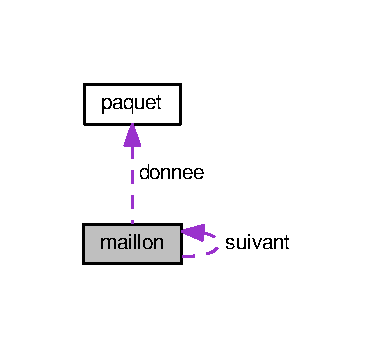
\includegraphics[width=180pt]{structmaillon__coll__graph}
\end{center}
\end{figure}
\subsection*{Data Fields}
\begin{DoxyCompactItemize}
\item 
\hyperlink{analyseur_8h_ac588becf5702254d8163c3386192122b}{Paquet} $\ast$ \hyperlink{structmaillon_ae3dd7456da37bc9d59abf1b042b61a5d}{donnee}
\item 
\hyperlink{analyseur_8h_a59ebf944443232737291655fc0b45ff2}{Liste} \hyperlink{structmaillon_a228be6326ce187047bca162b0f8db8c3}{suivant}
\end{DoxyCompactItemize}


\subsection{Field Documentation}
\index{maillon@{maillon}!donnee@{donnee}}
\index{donnee@{donnee}!maillon@{maillon}}
\subsubsection[{\texorpdfstring{donnee}{donnee}}]{\setlength{\rightskip}{0pt plus 5cm}{\bf Paquet}$\ast$ donnee}\hypertarget{structmaillon_ae3dd7456da37bc9d59abf1b042b61a5d}{}\label{structmaillon_ae3dd7456da37bc9d59abf1b042b61a5d}
\index{maillon@{maillon}!suivant@{suivant}}
\index{suivant@{suivant}!maillon@{maillon}}
\subsubsection[{\texorpdfstring{suivant}{suivant}}]{\setlength{\rightskip}{0pt plus 5cm}{\bf Liste} suivant}\hypertarget{structmaillon_a228be6326ce187047bca162b0f8db8c3}{}\label{structmaillon_a228be6326ce187047bca162b0f8db8c3}


The documentation for this struct was generated from the following file\+:\begin{DoxyCompactItemize}
\item 
src/\hyperlink{analyseur_8h}{analyseur.\+h}\end{DoxyCompactItemize}

\hypertarget{struct_option}{}\section{Option Struct Reference}
\label{struct_option}\index{Option@{Option}}


{\ttfamily \#include $<$analyseur.\+h$>$}

\subsection*{Data Fields}
\begin{DoxyCompactItemize}
\item 
char $\ast$ \hyperlink{struct_option_ab689c4ee257fccedce9922cb016c2e70}{i}
\item 
char $\ast$ \hyperlink{struct_option_ad736f700c72ff136cfb55439d8a11c7f}{o}
\item 
char $\ast$ \hyperlink{struct_option_ac2dd92a6e3aa88e63c9b7680aec3b02b}{f}
\item 
int \hyperlink{struct_option_ac8859e8c1ce357c4c8b37bbb1936ba1c}{v}
\end{DoxyCompactItemize}


\subsection{Field Documentation}
\index{Option@{Option}!f@{f}}
\index{f@{f}!Option@{Option}}
\subsubsection[{\texorpdfstring{f}{f}}]{\setlength{\rightskip}{0pt plus 5cm}char$\ast$ f}\hypertarget{struct_option_ac2dd92a6e3aa88e63c9b7680aec3b02b}{}\label{struct_option_ac2dd92a6e3aa88e63c9b7680aec3b02b}
\index{Option@{Option}!i@{i}}
\index{i@{i}!Option@{Option}}
\subsubsection[{\texorpdfstring{i}{i}}]{\setlength{\rightskip}{0pt plus 5cm}char$\ast$ i}\hypertarget{struct_option_ab689c4ee257fccedce9922cb016c2e70}{}\label{struct_option_ab689c4ee257fccedce9922cb016c2e70}
\index{Option@{Option}!o@{o}}
\index{o@{o}!Option@{Option}}
\subsubsection[{\texorpdfstring{o}{o}}]{\setlength{\rightskip}{0pt plus 5cm}char$\ast$ o}\hypertarget{struct_option_ad736f700c72ff136cfb55439d8a11c7f}{}\label{struct_option_ad736f700c72ff136cfb55439d8a11c7f}
\index{Option@{Option}!v@{v}}
\index{v@{v}!Option@{Option}}
\subsubsection[{\texorpdfstring{v}{v}}]{\setlength{\rightskip}{0pt plus 5cm}int v}\hypertarget{struct_option_ac8859e8c1ce357c4c8b37bbb1936ba1c}{}\label{struct_option_ac8859e8c1ce357c4c8b37bbb1936ba1c}


The documentation for this struct was generated from the following file\+:\begin{DoxyCompactItemize}
\item 
src/\hyperlink{analyseur_8h}{analyseur.\+h}\end{DoxyCompactItemize}

\hypertarget{structpaquet}{}\section{paquet Struct Reference}
\label{structpaquet}\index{paquet@{paquet}}


{\ttfamily \#include $<$analyseur.\+h$>$}

\subsection*{Data Fields}
\begin{DoxyCompactItemize}
\item 
int \hyperlink{structpaquet_a86cf672daa4e0ad11ad10efc894d19c8}{num}
\item 
bpf\+\_\+u\+\_\+int32 \hyperlink{structpaquet_a728f264db4f5cc304742565a2bcdbeea}{len}
\item 
\hyperlink{analyseur_8h_a8e361667cc667d5a11fd84869a8de384}{Date} $\ast$ \hyperlink{structpaquet_a73fc78564c9badbcea68f2f2331c74db}{date}
\end{DoxyCompactItemize}


\subsection{Field Documentation}
\index{paquet@{paquet}!date@{date}}
\index{date@{date}!paquet@{paquet}}
\subsubsection[{\texorpdfstring{date}{date}}]{\setlength{\rightskip}{0pt plus 5cm}{\bf Date}$\ast$ date}\hypertarget{structpaquet_a73fc78564c9badbcea68f2f2331c74db}{}\label{structpaquet_a73fc78564c9badbcea68f2f2331c74db}
\index{paquet@{paquet}!len@{len}}
\index{len@{len}!paquet@{paquet}}
\subsubsection[{\texorpdfstring{len}{len}}]{\setlength{\rightskip}{0pt plus 5cm}bpf\+\_\+u\+\_\+int32 len}\hypertarget{structpaquet_a728f264db4f5cc304742565a2bcdbeea}{}\label{structpaquet_a728f264db4f5cc304742565a2bcdbeea}
\index{paquet@{paquet}!num@{num}}
\index{num@{num}!paquet@{paquet}}
\subsubsection[{\texorpdfstring{num}{num}}]{\setlength{\rightskip}{0pt plus 5cm}int num}\hypertarget{structpaquet_a86cf672daa4e0ad11ad10efc894d19c8}{}\label{structpaquet_a86cf672daa4e0ad11ad10efc894d19c8}


The documentation for this struct was generated from the following file\+:\begin{DoxyCompactItemize}
\item 
src/\hyperlink{analyseur_8h}{analyseur.\+h}\end{DoxyCompactItemize}

\hypertarget{struct_user}{}\section{User Struct Reference}
\label{struct_user}\index{User@{User}}


{\ttfamily \#include $<$analyseur.\+h$>$}



Collaboration diagram for User\+:
\nopagebreak
\begin{figure}[H]
\begin{center}
\leavevmode
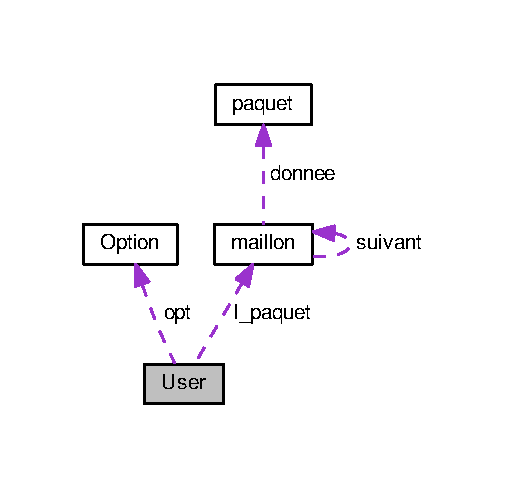
\includegraphics[width=243pt]{struct_user__coll__graph}
\end{center}
\end{figure}
\subsection*{Data Fields}
\begin{DoxyCompactItemize}
\item 
\hyperlink{struct_option}{Option} $\ast$ \hyperlink{struct_user_abf0b5d238619365cb08656c04e77bd28}{opt}
\item 
\hyperlink{analyseur_8h_a59ebf944443232737291655fc0b45ff2}{Liste} \hyperlink{struct_user_ad3b02cc08546fd807de16745eb9fc0ef}{l\+\_\+paquet}
\item 
int \hyperlink{struct_user_ac5d5fb856fd497fae6e967afd55bfab2}{nb\+\_\+paquet}
\end{DoxyCompactItemize}


\subsection{Field Documentation}
\index{User@{User}!l\+\_\+paquet@{l\+\_\+paquet}}
\index{l\+\_\+paquet@{l\+\_\+paquet}!User@{User}}
\subsubsection[{\texorpdfstring{l\+\_\+paquet}{l_paquet}}]{\setlength{\rightskip}{0pt plus 5cm}{\bf Liste} l\+\_\+paquet}\hypertarget{struct_user_ad3b02cc08546fd807de16745eb9fc0ef}{}\label{struct_user_ad3b02cc08546fd807de16745eb9fc0ef}
\index{User@{User}!nb\+\_\+paquet@{nb\+\_\+paquet}}
\index{nb\+\_\+paquet@{nb\+\_\+paquet}!User@{User}}
\subsubsection[{\texorpdfstring{nb\+\_\+paquet}{nb_paquet}}]{\setlength{\rightskip}{0pt plus 5cm}int nb\+\_\+paquet}\hypertarget{struct_user_ac5d5fb856fd497fae6e967afd55bfab2}{}\label{struct_user_ac5d5fb856fd497fae6e967afd55bfab2}
\index{User@{User}!opt@{opt}}
\index{opt@{opt}!User@{User}}
\subsubsection[{\texorpdfstring{opt}{opt}}]{\setlength{\rightskip}{0pt plus 5cm}{\bf Option}$\ast$ opt}\hypertarget{struct_user_abf0b5d238619365cb08656c04e77bd28}{}\label{struct_user_abf0b5d238619365cb08656c04e77bd28}


The documentation for this struct was generated from the following file\+:\begin{DoxyCompactItemize}
\item 
src/\hyperlink{analyseur_8h}{analyseur.\+h}\end{DoxyCompactItemize}

\chapter{File Documentation}
\hypertarget{analyseur_8c}{}\section{src/analyseur.c File Reference}
\label{analyseur_8c}\index{src/analyseur.\+c@{src/analyseur.\+c}}


Fonctions principales.  


{\ttfamily \#include \char`\"{}analyseur.\+h\char`\"{}}\\*
Include dependency graph for analyseur.\+c\+:
\nopagebreak
\begin{figure}[H]
\begin{center}
\leavevmode
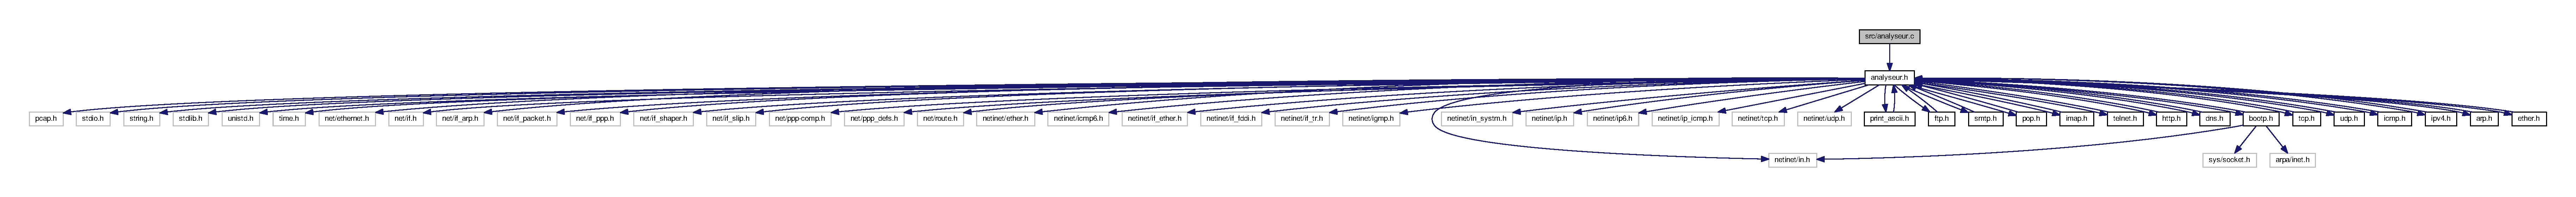
\includegraphics[width=350pt]{analyseur_8c__incl}
\end{center}
\end{figure}
\subsection*{Functions}
\begin{DoxyCompactItemize}
\item 
\hyperlink{analyseur_8h_a59ebf944443232737291655fc0b45ff2}{Liste} \hyperlink{analyseur_8c_a9e11e88b64a6173035fbc3693b792e42}{cons} (\hyperlink{analyseur_8h_a59ebf944443232737291655fc0b45ff2}{Liste} l, \hyperlink{analyseur_8h_ac588becf5702254d8163c3386192122b}{Paquet} $\ast$nvelt)
\begin{DoxyCompactList}\small\item\em Constructeur de liste de paquet. \end{DoxyCompactList}\item 
void \hyperlink{analyseur_8c_a5dc2f4ebaf124e7bf53b56c7477199a8}{callback} (u\+\_\+char $\ast$user, const struct pcap\+\_\+pkthdr $\ast$h, const u\+\_\+char $\ast$bytes)
\begin{DoxyCompactList}\small\item\em Fonction de callback appelé à chaque lecture d\textquotesingle{}un nouveau paquet. \end{DoxyCompactList}\item 
void \hyperlink{analyseur_8c_aba24889b9dabf8bcd576c88285c7bd75}{affichage\+\_\+option} (\hyperlink{struct_option}{Option} $\ast$opt)
\begin{DoxyCompactList}\small\item\em Affiche les options et les arguments passés à l\textquotesingle{}exécutable. \end{DoxyCompactList}\item 
void \hyperlink{analyseur_8c_a29cc98853004fea19143b99c2611c197}{set\+\_\+option} (\hyperlink{struct_option}{Option} $\ast$option, int argc, char $\ast$argv\mbox{[}$\,$\mbox{]})
\begin{DoxyCompactList}\small\item\em Reconnais les options passés à l\textquotesingle{}exécutable. \end{DoxyCompactList}\item 
void \hyperlink{analyseur_8c_a999b77002afb0d1895733855d87d9dd3}{start\+\_\+analyse\+\_\+online} (\hyperlink{struct_user}{User} $\ast$user)
\begin{DoxyCompactList}\small\item\em Lance l\textquotesingle{}analyse en mode online. \end{DoxyCompactList}\item 
void \hyperlink{analyseur_8c_a4b115c29c5b2ec60686bd113005a2ba4}{start\+\_\+analyse\+\_\+offline} (\hyperlink{struct_user}{User} $\ast$user)
\begin{DoxyCompactList}\small\item\em Lance l\textquotesingle{}analyse en mode offline. \end{DoxyCompactList}\item 
void \hyperlink{analyseur_8c_aa786d2dda18985d6ae1c20b425a0b1b4}{free\+\_\+l\+\_\+paquet} (\hyperlink{analyseur_8h_a59ebf944443232737291655fc0b45ff2}{Liste} l\+\_\+paquet)
\begin{DoxyCompactList}\small\item\em Libère la mémoire. \end{DoxyCompactList}\item 
int \hyperlink{analyseur_8c_a0ddf1224851353fc92bfbff6f499fa97}{main} (int argc, char $\ast$argv\mbox{[}$\,$\mbox{]})
\end{DoxyCompactItemize}


\subsection{Detailed Description}
Fonctions principales. 

\begin{DoxyAuthor}{Author}
De La Roche Constantin 
\end{DoxyAuthor}
\begin{DoxyVersion}{Version}
1 
\end{DoxyVersion}
\begin{DoxyDate}{Date}
16/12/16
\end{DoxyDate}
Contient tout ce qui concerne pcap 

\subsection{Function Documentation}
\index{analyseur.\+c@{analyseur.\+c}!affichage\+\_\+option@{affichage\+\_\+option}}
\index{affichage\+\_\+option@{affichage\+\_\+option}!analyseur.\+c@{analyseur.\+c}}
\subsubsection[{\texorpdfstring{affichage\+\_\+option(\+Option $\ast$opt)}{affichage_option(Option *opt)}}]{\setlength{\rightskip}{0pt plus 5cm}void affichage\+\_\+option (
\begin{DoxyParamCaption}
\item[{{\bf Option} $\ast$}]{opt}
\end{DoxyParamCaption}
)}\hypertarget{analyseur_8c_aba24889b9dabf8bcd576c88285c7bd75}{}\label{analyseur_8c_aba24889b9dabf8bcd576c88285c7bd75}


Affiche les options et les arguments passés à l\textquotesingle{}exécutable. 


\begin{DoxyParams}{Parameters}
{\em opt} & Contient les options \\
\hline
\end{DoxyParams}
\index{analyseur.\+c@{analyseur.\+c}!callback@{callback}}
\index{callback@{callback}!analyseur.\+c@{analyseur.\+c}}
\subsubsection[{\texorpdfstring{callback(u\+\_\+char $\ast$user, const struct pcap\+\_\+pkthdr $\ast$h, const u\+\_\+char $\ast$bytes)}{callback(u_char *user, const struct pcap_pkthdr *h, const u_char *bytes)}}]{\setlength{\rightskip}{0pt plus 5cm}void callback (
\begin{DoxyParamCaption}
\item[{u\+\_\+char $\ast$}]{user, }
\item[{const struct pcap\+\_\+pkthdr $\ast$}]{h, }
\item[{const u\+\_\+char $\ast$}]{bytes}
\end{DoxyParamCaption}
)}\hypertarget{analyseur_8c_a5dc2f4ebaf124e7bf53b56c7477199a8}{}\label{analyseur_8c_a5dc2f4ebaf124e7bf53b56c7477199a8}


Fonction de callback appelé à chaque lecture d\textquotesingle{}un nouveau paquet. 

Le contenue du paquet contenu dans bytes est forward à la fonction analyse\+\_\+ethenert qui analyse l\textquotesingle{}entête ethernet. On crée un nouveau paquet. On met à jour la liste des paquets lus. On met à jour le pointeur user


\begin{DoxyParams}{Parameters}
{\em user} & Véhicule les informations \\
\hline
{\em pcap\+\_\+pkthdr} & Unused \\
\hline
{\em bytes} & Contenu du paquet \\
\hline
\end{DoxyParams}
\index{analyseur.\+c@{analyseur.\+c}!cons@{cons}}
\index{cons@{cons}!analyseur.\+c@{analyseur.\+c}}
\subsubsection[{\texorpdfstring{cons(\+Liste l, Paquet $\ast$nvelt)}{cons(Liste l, Paquet *nvelt)}}]{\setlength{\rightskip}{0pt plus 5cm}{\bf Liste} cons (
\begin{DoxyParamCaption}
\item[{{\bf Liste}}]{l, }
\item[{{\bf Paquet} $\ast$}]{nvelt}
\end{DoxyParamCaption}
)}\hypertarget{analyseur_8c_a9e11e88b64a6173035fbc3693b792e42}{}\label{analyseur_8c_a9e11e88b64a6173035fbc3693b792e42}


Constructeur de liste de paquet. 

Ajout un paquet à la liste des paquets lus. Utilisé pour l\textquotesingle{}affichage avec clutter.


\begin{DoxyParams}{Parameters}
{\em l} & Liste des paquets \\
\hline
{\em nvelt} & Paquet à ajouter à la liste\\
\hline
\end{DoxyParams}
\begin{DoxyReturn}{Returns}
La liste augmentée. 
\end{DoxyReturn}
\index{analyseur.\+c@{analyseur.\+c}!free\+\_\+l\+\_\+paquet@{free\+\_\+l\+\_\+paquet}}
\index{free\+\_\+l\+\_\+paquet@{free\+\_\+l\+\_\+paquet}!analyseur.\+c@{analyseur.\+c}}
\subsubsection[{\texorpdfstring{free\+\_\+l\+\_\+paquet(\+Liste l\+\_\+paquet)}{free_l_paquet(Liste l_paquet)}}]{\setlength{\rightskip}{0pt plus 5cm}void free\+\_\+l\+\_\+paquet (
\begin{DoxyParamCaption}
\item[{{\bf Liste}}]{l\+\_\+paquet}
\end{DoxyParamCaption}
)}\hypertarget{analyseur_8c_aa786d2dda18985d6ae1c20b425a0b1b4}{}\label{analyseur_8c_aa786d2dda18985d6ae1c20b425a0b1b4}


Libère la mémoire. 

Delete la liste des paquets


\begin{DoxyParams}{Parameters}
{\em l\+\_\+paquet} & Liste des paquets à effacer \\
\hline
\end{DoxyParams}
\index{analyseur.\+c@{analyseur.\+c}!main@{main}}
\index{main@{main}!analyseur.\+c@{analyseur.\+c}}
\subsubsection[{\texorpdfstring{main(int argc, char $\ast$argv[])}{main(int argc, char *argv[])}}]{\setlength{\rightskip}{0pt plus 5cm}int main (
\begin{DoxyParamCaption}
\item[{int}]{argc, }
\item[{char $\ast$}]{argv\mbox{[}$\,$\mbox{]}}
\end{DoxyParamCaption}
)}\hypertarget{analyseur_8c_a0ddf1224851353fc92bfbff6f499fa97}{}\label{analyseur_8c_a0ddf1224851353fc92bfbff6f499fa97}
\index{analyseur.\+c@{analyseur.\+c}!set\+\_\+option@{set\+\_\+option}}
\index{set\+\_\+option@{set\+\_\+option}!analyseur.\+c@{analyseur.\+c}}
\subsubsection[{\texorpdfstring{set\+\_\+option(\+Option $\ast$option, int argc, char $\ast$argv[])}{set_option(Option *option, int argc, char *argv[])}}]{\setlength{\rightskip}{0pt plus 5cm}void set\+\_\+option (
\begin{DoxyParamCaption}
\item[{{\bf Option} $\ast$}]{option, }
\item[{int}]{argc, }
\item[{char $\ast$}]{argv\mbox{[}$\,$\mbox{]}}
\end{DoxyParamCaption}
)}\hypertarget{analyseur_8c_a29cc98853004fea19143b99c2611c197}{}\label{analyseur_8c_a29cc98853004fea19143b99c2611c197}


Reconnais les options passés à l\textquotesingle{}exécutable. 

Reconnais et initialise les options passés en argument à l\textquotesingle{}exécutable.


\begin{DoxyParams}{Parameters}
{\em option} & Pointeur qui contiendra les options \\
\hline
{\em argc} & main \\
\hline
{\em argv} & main \\
\hline
\end{DoxyParams}
\index{analyseur.\+c@{analyseur.\+c}!start\+\_\+analyse\+\_\+offline@{start\+\_\+analyse\+\_\+offline}}
\index{start\+\_\+analyse\+\_\+offline@{start\+\_\+analyse\+\_\+offline}!analyseur.\+c@{analyseur.\+c}}
\subsubsection[{\texorpdfstring{start\+\_\+analyse\+\_\+offline(\+User $\ast$user)}{start_analyse_offline(User *user)}}]{\setlength{\rightskip}{0pt plus 5cm}void start\+\_\+analyse\+\_\+offline (
\begin{DoxyParamCaption}
\item[{{\bf User} $\ast$}]{user}
\end{DoxyParamCaption}
)}\hypertarget{analyseur_8c_a4b115c29c5b2ec60686bd113005a2ba4}{}\label{analyseur_8c_a4b115c29c5b2ec60686bd113005a2ba4}


Lance l\textquotesingle{}analyse en mode offline. 

Capture à partir d\textquotesingle{}un fichier.


\begin{DoxyParams}{Parameters}
{\em user} & \\
\hline
\end{DoxyParams}
\index{analyseur.\+c@{analyseur.\+c}!start\+\_\+analyse\+\_\+online@{start\+\_\+analyse\+\_\+online}}
\index{start\+\_\+analyse\+\_\+online@{start\+\_\+analyse\+\_\+online}!analyseur.\+c@{analyseur.\+c}}
\subsubsection[{\texorpdfstring{start\+\_\+analyse\+\_\+online(\+User $\ast$user)}{start_analyse_online(User *user)}}]{\setlength{\rightskip}{0pt plus 5cm}void start\+\_\+analyse\+\_\+online (
\begin{DoxyParamCaption}
\item[{{\bf User} $\ast$}]{user}
\end{DoxyParamCaption}
)}\hypertarget{analyseur_8c_a999b77002afb0d1895733855d87d9dd3}{}\label{analyseur_8c_a999b77002afb0d1895733855d87d9dd3}


Lance l\textquotesingle{}analyse en mode online. 

Capture en temps réel


\begin{DoxyParams}{Parameters}
{\em user} & \\
\hline
\end{DoxyParams}

\hypertarget{analyseur_8h}{}\section{src/analyseur.h File Reference}
\label{analyseur_8h}\index{src/analyseur.\+h@{src/analyseur.\+h}}
{\ttfamily \#include $<$pcap.\+h$>$}\\*
{\ttfamily \#include $<$stdio.\+h$>$}\\*
{\ttfamily \#include $<$string.\+h$>$}\\*
{\ttfamily \#include $<$stdlib.\+h$>$}\\*
{\ttfamily \#include $<$unistd.\+h$>$}\\*
{\ttfamily \#include $<$time.\+h$>$}\\*
{\ttfamily \#include $<$net/ethernet.\+h$>$}\\*
{\ttfamily \#include $<$net/if.\+h$>$}\\*
{\ttfamily \#include $<$net/if\+\_\+arp.\+h$>$}\\*
{\ttfamily \#include $<$net/if\+\_\+packet.\+h$>$}\\*
{\ttfamily \#include $<$net/if\+\_\+ppp.\+h$>$}\\*
{\ttfamily \#include $<$net/if\+\_\+shaper.\+h$>$}\\*
{\ttfamily \#include $<$net/if\+\_\+slip.\+h$>$}\\*
{\ttfamily \#include $<$net/ppp-\/comp.\+h$>$}\\*
{\ttfamily \#include $<$net/ppp\+\_\+defs.\+h$>$}\\*
{\ttfamily \#include $<$net/route.\+h$>$}\\*
{\ttfamily \#include $<$netinet/ether.\+h$>$}\\*
{\ttfamily \#include $<$netinet/icmp6.\+h$>$}\\*
{\ttfamily \#include $<$netinet/if\+\_\+ether.\+h$>$}\\*
{\ttfamily \#include $<$netinet/if\+\_\+fddi.\+h$>$}\\*
{\ttfamily \#include $<$netinet/if\+\_\+tr.\+h$>$}\\*
{\ttfamily \#include $<$netinet/igmp.\+h$>$}\\*
{\ttfamily \#include $<$netinet/in.\+h$>$}\\*
{\ttfamily \#include $<$netinet/in\+\_\+systm.\+h$>$}\\*
{\ttfamily \#include $<$netinet/ip.\+h$>$}\\*
{\ttfamily \#include $<$netinet/ip6.\+h$>$}\\*
{\ttfamily \#include $<$netinet/ip\+\_\+icmp.\+h$>$}\\*
{\ttfamily \#include $<$netinet/tcp.\+h$>$}\\*
{\ttfamily \#include $<$netinet/udp.\+h$>$}\\*
{\ttfamily \#include \char`\"{}print\+\_\+ascii.\+h\char`\"{}}\\*
{\ttfamily \#include \char`\"{}ftp.\+h\char`\"{}}\\*
{\ttfamily \#include \char`\"{}smtp.\+h\char`\"{}}\\*
{\ttfamily \#include \char`\"{}pop.\+h\char`\"{}}\\*
{\ttfamily \#include \char`\"{}imap.\+h\char`\"{}}\\*
{\ttfamily \#include \char`\"{}telnet.\+h\char`\"{}}\\*
{\ttfamily \#include \char`\"{}http.\+h\char`\"{}}\\*
{\ttfamily \#include \char`\"{}dns.\+h\char`\"{}}\\*
{\ttfamily \#include \char`\"{}bootp.\+h\char`\"{}}\\*
{\ttfamily \#include \char`\"{}tcp.\+h\char`\"{}}\\*
{\ttfamily \#include \char`\"{}udp.\+h\char`\"{}}\\*
{\ttfamily \#include \char`\"{}icmp.\+h\char`\"{}}\\*
{\ttfamily \#include \char`\"{}ipv4.\+h\char`\"{}}\\*
{\ttfamily \#include \char`\"{}arp.\+h\char`\"{}}\\*
{\ttfamily \#include \char`\"{}ether.\+h\char`\"{}}\\*
Include dependency graph for analyseur.\+h\+:
\nopagebreak
\begin{figure}[H]
\begin{center}
\leavevmode
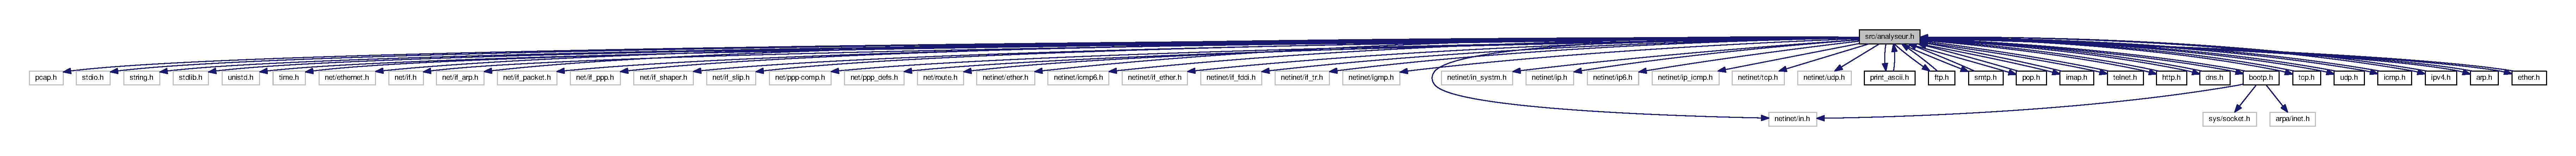
\includegraphics[width=350pt]{analyseur_8h__incl}
\end{center}
\end{figure}
This graph shows which files directly or indirectly include this file\+:
\nopagebreak
\begin{figure}[H]
\begin{center}
\leavevmode
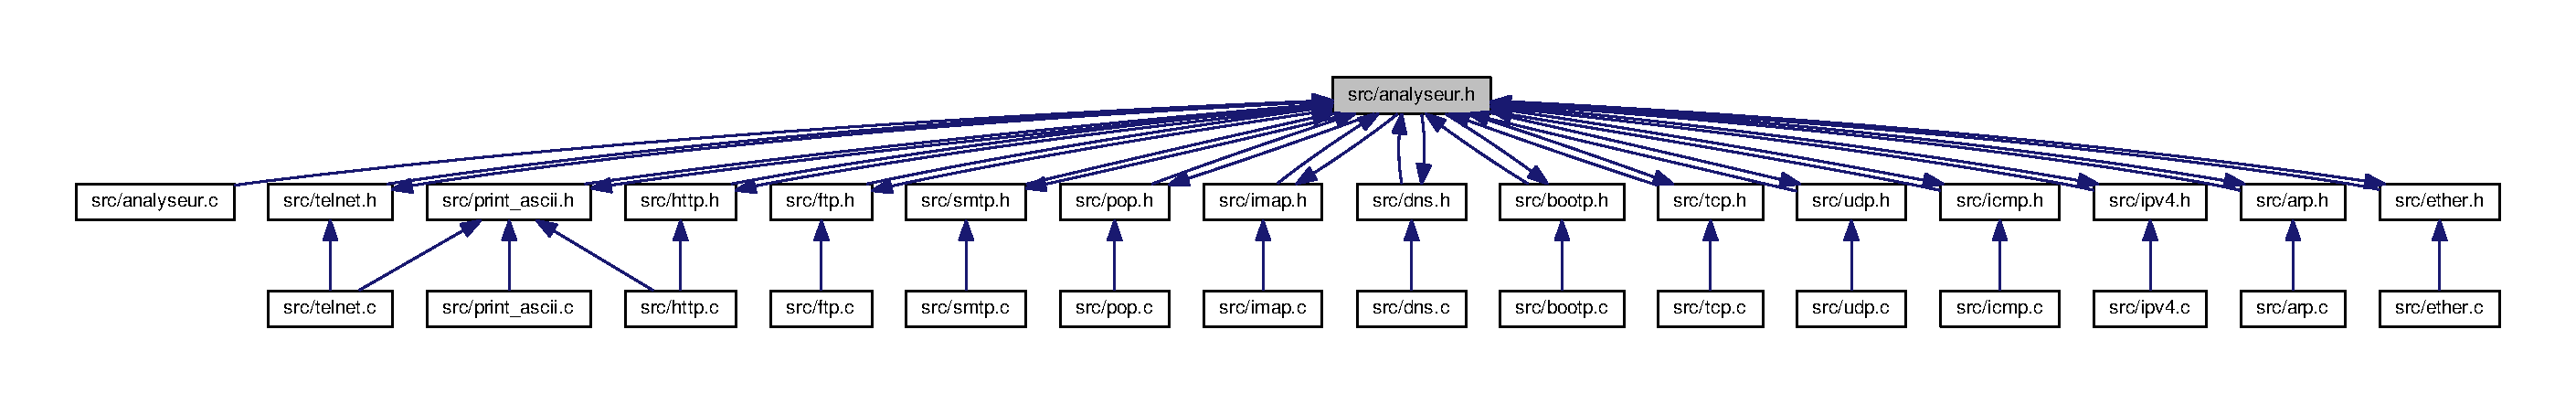
\includegraphics[width=350pt]{analyseur_8h__dep__incl}
\end{center}
\end{figure}
\subsection*{Data Structures}
\begin{DoxyCompactItemize}
\item 
struct \hyperlink{struct_option}{Option}
\item 
struct \hyperlink{structpaquet}{paquet}
\item 
struct \hyperlink{structmaillon}{maillon}
\item 
struct \hyperlink{struct_user}{User}
\item 
struct \hyperlink{struct__arphdr}{\+\_\+arphdr}
\end{DoxyCompactItemize}
\subsection*{Macros}
\begin{DoxyCompactItemize}
\item 
\#define \hyperlink{analyseur_8h_aabcb2d6536b6c0ab41f99493c911489b}{couleur}(param)~printf(\char`\"{}\textbackslash{}033\mbox{[}\%sm\char`\"{},param)
\end{DoxyCompactItemize}
\subsection*{Typedefs}
\begin{DoxyCompactItemize}
\item 
typedef struct tm \hyperlink{analyseur_8h_a8e361667cc667d5a11fd84869a8de384}{Date}
\item 
typedef struct \hyperlink{struct_option}{Option} \hyperlink{analyseur_8h_ab04ea1b4cb7ae1ddc63e3f014cae5515}{Option}
\item 
typedef struct \hyperlink{structpaquet}{paquet} \hyperlink{analyseur_8h_ac588becf5702254d8163c3386192122b}{Paquet}
\item 
typedef struct \hyperlink{structmaillon}{maillon} $\ast$ \hyperlink{analyseur_8h_a59ebf944443232737291655fc0b45ff2}{Liste}
\item 
typedef struct \hyperlink{struct_user}{User} \hyperlink{analyseur_8h_aebb0f8a8bd00b8afba0e5abcf5b559c7}{User}
\item 
typedef struct ether\+\_\+header \hyperlink{analyseur_8h_ad90aff77137032898c538ebab55e5c76}{Ether\+Hdr}
\item 
typedef struct \hyperlink{struct__arphdr}{\+\_\+arphdr} \hyperlink{analyseur_8h_ad6a591e8b3d92a7c1cd97fed01ff92c3}{Arp\+Hdr}
\item 
typedef struct iphdr \hyperlink{analyseur_8h_a6fc2e7c521fb740fdb7d8b8c16698324}{Ip\+Hdr}
\item 
typedef struct tcphdr \hyperlink{analyseur_8h_a0a79f5959e54cfe5f13ff5207c59152e}{Tcp\+Hdr}
\item 
typedef struct udphdr \hyperlink{analyseur_8h_a450cdf739df0886778ce02bd0ab86b63}{Udp\+Hdr}
\item 
typedef struct icmphdr \hyperlink{analyseur_8h_ac69a3725cff99f912ce0d4281b5b4ea7}{Icmp\+Hdr}
\item 
typedef struct \hyperlink{structbootp}{bootp} \hyperlink{analyseur_8h_abda6a1c8d85a6aab6c4819fe6e97c2d3}{Bootp}
\end{DoxyCompactItemize}
\subsection*{Functions}
\begin{DoxyCompactItemize}
\item 
\hyperlink{analyseur_8h_a59ebf944443232737291655fc0b45ff2}{Liste} \hyperlink{analyseur_8h_a9e11e88b64a6173035fbc3693b792e42}{cons} (\hyperlink{analyseur_8h_a59ebf944443232737291655fc0b45ff2}{Liste} l, \hyperlink{analyseur_8h_ac588becf5702254d8163c3386192122b}{Paquet} $\ast$nvelt)
\begin{DoxyCompactList}\small\item\em Constructeur de liste de paquet. \end{DoxyCompactList}\item 
void \hyperlink{analyseur_8h_a0a9b0fae800c2639d0dfa1858d25467e}{start\+\_\+analyse} (\hyperlink{struct_user}{User} $\ast$user)
\end{DoxyCompactItemize}


\subsection{Macro Definition Documentation}
\index{analyseur.\+h@{analyseur.\+h}!couleur@{couleur}}
\index{couleur@{couleur}!analyseur.\+h@{analyseur.\+h}}
\subsubsection[{\texorpdfstring{couleur}{couleur}}]{\setlength{\rightskip}{0pt plus 5cm}\#define couleur(
\begin{DoxyParamCaption}
\item[{}]{param}
\end{DoxyParamCaption}
)~printf(\char`\"{}\textbackslash{}033\mbox{[}\%sm\char`\"{},param)}\hypertarget{analyseur_8h_aabcb2d6536b6c0ab41f99493c911489b}{}\label{analyseur_8h_aabcb2d6536b6c0ab41f99493c911489b}


\subsection{Typedef Documentation}
\index{analyseur.\+h@{analyseur.\+h}!Arp\+Hdr@{Arp\+Hdr}}
\index{Arp\+Hdr@{Arp\+Hdr}!analyseur.\+h@{analyseur.\+h}}
\subsubsection[{\texorpdfstring{Arp\+Hdr}{ArpHdr}}]{\setlength{\rightskip}{0pt plus 5cm}typedef struct {\bf \+\_\+arphdr} {\bf Arp\+Hdr}}\hypertarget{analyseur_8h_ad6a591e8b3d92a7c1cd97fed01ff92c3}{}\label{analyseur_8h_ad6a591e8b3d92a7c1cd97fed01ff92c3}
\index{analyseur.\+h@{analyseur.\+h}!Bootp@{Bootp}}
\index{Bootp@{Bootp}!analyseur.\+h@{analyseur.\+h}}
\subsubsection[{\texorpdfstring{Bootp}{Bootp}}]{\setlength{\rightskip}{0pt plus 5cm}typedef struct {\bf bootp} {\bf Bootp}}\hypertarget{analyseur_8h_abda6a1c8d85a6aab6c4819fe6e97c2d3}{}\label{analyseur_8h_abda6a1c8d85a6aab6c4819fe6e97c2d3}
\index{analyseur.\+h@{analyseur.\+h}!Date@{Date}}
\index{Date@{Date}!analyseur.\+h@{analyseur.\+h}}
\subsubsection[{\texorpdfstring{Date}{Date}}]{\setlength{\rightskip}{0pt plus 5cm}typedef struct tm {\bf Date}}\hypertarget{analyseur_8h_a8e361667cc667d5a11fd84869a8de384}{}\label{analyseur_8h_a8e361667cc667d5a11fd84869a8de384}
\index{analyseur.\+h@{analyseur.\+h}!Ether\+Hdr@{Ether\+Hdr}}
\index{Ether\+Hdr@{Ether\+Hdr}!analyseur.\+h@{analyseur.\+h}}
\subsubsection[{\texorpdfstring{Ether\+Hdr}{EtherHdr}}]{\setlength{\rightskip}{0pt plus 5cm}typedef struct ether\+\_\+header {\bf Ether\+Hdr}}\hypertarget{analyseur_8h_ad90aff77137032898c538ebab55e5c76}{}\label{analyseur_8h_ad90aff77137032898c538ebab55e5c76}
\index{analyseur.\+h@{analyseur.\+h}!Icmp\+Hdr@{Icmp\+Hdr}}
\index{Icmp\+Hdr@{Icmp\+Hdr}!analyseur.\+h@{analyseur.\+h}}
\subsubsection[{\texorpdfstring{Icmp\+Hdr}{IcmpHdr}}]{\setlength{\rightskip}{0pt plus 5cm}typedef struct icmphdr {\bf Icmp\+Hdr}}\hypertarget{analyseur_8h_ac69a3725cff99f912ce0d4281b5b4ea7}{}\label{analyseur_8h_ac69a3725cff99f912ce0d4281b5b4ea7}
\index{analyseur.\+h@{analyseur.\+h}!Ip\+Hdr@{Ip\+Hdr}}
\index{Ip\+Hdr@{Ip\+Hdr}!analyseur.\+h@{analyseur.\+h}}
\subsubsection[{\texorpdfstring{Ip\+Hdr}{IpHdr}}]{\setlength{\rightskip}{0pt plus 5cm}typedef struct iphdr {\bf Ip\+Hdr}}\hypertarget{analyseur_8h_a6fc2e7c521fb740fdb7d8b8c16698324}{}\label{analyseur_8h_a6fc2e7c521fb740fdb7d8b8c16698324}
\index{analyseur.\+h@{analyseur.\+h}!Liste@{Liste}}
\index{Liste@{Liste}!analyseur.\+h@{analyseur.\+h}}
\subsubsection[{\texorpdfstring{Liste}{Liste}}]{\setlength{\rightskip}{0pt plus 5cm}typedef struct {\bf maillon}$\ast$ {\bf Liste}}\hypertarget{analyseur_8h_a59ebf944443232737291655fc0b45ff2}{}\label{analyseur_8h_a59ebf944443232737291655fc0b45ff2}
\index{analyseur.\+h@{analyseur.\+h}!Option@{Option}}
\index{Option@{Option}!analyseur.\+h@{analyseur.\+h}}
\subsubsection[{\texorpdfstring{Option}{Option}}]{\setlength{\rightskip}{0pt plus 5cm}typedef struct {\bf Option} {\bf Option}}\hypertarget{analyseur_8h_ab04ea1b4cb7ae1ddc63e3f014cae5515}{}\label{analyseur_8h_ab04ea1b4cb7ae1ddc63e3f014cae5515}
\index{analyseur.\+h@{analyseur.\+h}!Paquet@{Paquet}}
\index{Paquet@{Paquet}!analyseur.\+h@{analyseur.\+h}}
\subsubsection[{\texorpdfstring{Paquet}{Paquet}}]{\setlength{\rightskip}{0pt plus 5cm}typedef struct {\bf paquet} {\bf Paquet}}\hypertarget{analyseur_8h_ac588becf5702254d8163c3386192122b}{}\label{analyseur_8h_ac588becf5702254d8163c3386192122b}
\index{analyseur.\+h@{analyseur.\+h}!Tcp\+Hdr@{Tcp\+Hdr}}
\index{Tcp\+Hdr@{Tcp\+Hdr}!analyseur.\+h@{analyseur.\+h}}
\subsubsection[{\texorpdfstring{Tcp\+Hdr}{TcpHdr}}]{\setlength{\rightskip}{0pt plus 5cm}typedef struct tcphdr {\bf Tcp\+Hdr}}\hypertarget{analyseur_8h_a0a79f5959e54cfe5f13ff5207c59152e}{}\label{analyseur_8h_a0a79f5959e54cfe5f13ff5207c59152e}
\index{analyseur.\+h@{analyseur.\+h}!Udp\+Hdr@{Udp\+Hdr}}
\index{Udp\+Hdr@{Udp\+Hdr}!analyseur.\+h@{analyseur.\+h}}
\subsubsection[{\texorpdfstring{Udp\+Hdr}{UdpHdr}}]{\setlength{\rightskip}{0pt plus 5cm}typedef struct udphdr {\bf Udp\+Hdr}}\hypertarget{analyseur_8h_a450cdf739df0886778ce02bd0ab86b63}{}\label{analyseur_8h_a450cdf739df0886778ce02bd0ab86b63}
\index{analyseur.\+h@{analyseur.\+h}!User@{User}}
\index{User@{User}!analyseur.\+h@{analyseur.\+h}}
\subsubsection[{\texorpdfstring{User}{User}}]{\setlength{\rightskip}{0pt plus 5cm}typedef struct {\bf User} {\bf User}}\hypertarget{analyseur_8h_aebb0f8a8bd00b8afba0e5abcf5b559c7}{}\label{analyseur_8h_aebb0f8a8bd00b8afba0e5abcf5b559c7}


\subsection{Function Documentation}
\index{analyseur.\+h@{analyseur.\+h}!cons@{cons}}
\index{cons@{cons}!analyseur.\+h@{analyseur.\+h}}
\subsubsection[{\texorpdfstring{cons(\+Liste l, Paquet $\ast$nvelt)}{cons(Liste l, Paquet *nvelt)}}]{\setlength{\rightskip}{0pt plus 5cm}{\bf Liste} cons (
\begin{DoxyParamCaption}
\item[{{\bf Liste}}]{l, }
\item[{{\bf Paquet} $\ast$}]{nvelt}
\end{DoxyParamCaption}
)}\hypertarget{analyseur_8h_a9e11e88b64a6173035fbc3693b792e42}{}\label{analyseur_8h_a9e11e88b64a6173035fbc3693b792e42}


Constructeur de liste de paquet. 

Ajout un paquet à la liste des paquets lus. Utilisé pour l\textquotesingle{}affichage avec clutter.


\begin{DoxyParams}{Parameters}
{\em l} & Liste des paquets \\
\hline
{\em nvelt} & Paquet à ajouter à la liste\\
\hline
\end{DoxyParams}
\begin{DoxyReturn}{Returns}
La liste augmentée. 
\end{DoxyReturn}
\index{analyseur.\+h@{analyseur.\+h}!start\+\_\+analyse@{start\+\_\+analyse}}
\index{start\+\_\+analyse@{start\+\_\+analyse}!analyseur.\+h@{analyseur.\+h}}
\subsubsection[{\texorpdfstring{start\+\_\+analyse(\+User $\ast$user)}{start_analyse(User *user)}}]{\setlength{\rightskip}{0pt plus 5cm}void start\+\_\+analyse (
\begin{DoxyParamCaption}
\item[{{\bf User} $\ast$}]{user}
\end{DoxyParamCaption}
)}\hypertarget{analyseur_8h_a0a9b0fae800c2639d0dfa1858d25467e}{}\label{analyseur_8h_a0a9b0fae800c2639d0dfa1858d25467e}

\hypertarget{arp_8c}{}\section{src/arp.c File Reference}
\label{arp_8c}\index{src/arp.\+c@{src/arp.\+c}}
{\ttfamily \#include \char`\"{}arp.\+h\char`\"{}}\\*
Include dependency graph for arp.\+c\+:
\nopagebreak
\begin{figure}[H]
\begin{center}
\leavevmode
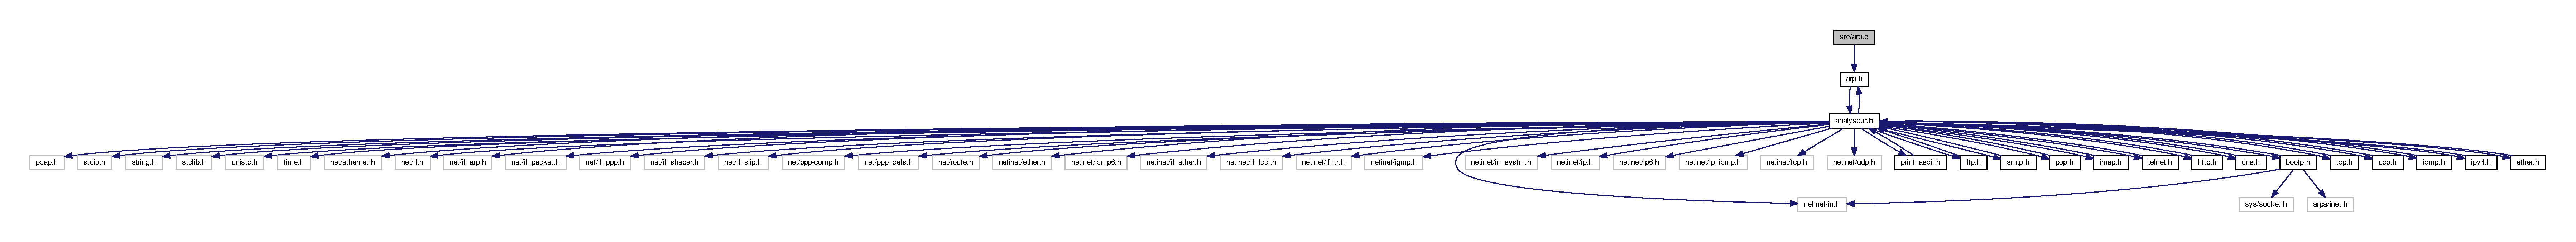
\includegraphics[width=350pt]{arp_8c__incl}
\end{center}
\end{figure}
\subsection*{Functions}
\begin{DoxyCompactItemize}
\item 
void \hyperlink{arp_8c_a8f7ef5a1b347d42f4a45d9cb9ad576d2}{affichage\+\_\+arp} (\hyperlink{struct_user}{User} $\ast$user, \hyperlink{analyseur_8h_ad6a591e8b3d92a7c1cd97fed01ff92c3}{Arp\+Hdr} $\ast$arphdr)
\begin{DoxyCompactList}\small\item\em Affiche les information sur le header. \end{DoxyCompactList}\item 
void \hyperlink{arp_8c_af2c37cf12e56fd074bc1d35e46b9536f}{analyse\+\_\+arp} (\hyperlink{struct_user}{User} $\ast$user, const u\+\_\+char $\ast$bytes)
\end{DoxyCompactItemize}


\subsection{Function Documentation}
\index{arp.\+c@{arp.\+c}!affichage\+\_\+arp@{affichage\+\_\+arp}}
\index{affichage\+\_\+arp@{affichage\+\_\+arp}!arp.\+c@{arp.\+c}}
\subsubsection[{\texorpdfstring{affichage\+\_\+arp(\+User $\ast$user, Arp\+Hdr $\ast$arphdr)}{affichage_arp(User *user, ArpHdr *arphdr)}}]{\setlength{\rightskip}{0pt plus 5cm}void affichage\+\_\+arp (
\begin{DoxyParamCaption}
\item[{{\bf User} $\ast$}]{user, }
\item[{{\bf Arp\+Hdr} $\ast$}]{arphdr}
\end{DoxyParamCaption}
)}\hypertarget{arp_8c_a8f7ef5a1b347d42f4a45d9cb9ad576d2}{}\label{arp_8c_a8f7ef5a1b347d42f4a45d9cb9ad576d2}


Affiche les information sur le header. 

Affichage en fonction de la verbosité


\begin{DoxyParams}{Parameters}
{\em user} & \\
\hline
{\em arphdr} & \\
\hline
\end{DoxyParams}
\index{arp.\+c@{arp.\+c}!analyse\+\_\+arp@{analyse\+\_\+arp}}
\index{analyse\+\_\+arp@{analyse\+\_\+arp}!arp.\+c@{arp.\+c}}
\subsubsection[{\texorpdfstring{analyse\+\_\+arp(\+User $\ast$user, const u\+\_\+char $\ast$bytes)}{analyse_arp(User *user, const u_char *bytes)}}]{\setlength{\rightskip}{0pt plus 5cm}void analyse\+\_\+arp (
\begin{DoxyParamCaption}
\item[{{\bf User} $\ast$}]{user, }
\item[{const u\+\_\+char $\ast$}]{bytes}
\end{DoxyParamCaption}
)}\hypertarget{arp_8c_af2c37cf12e56fd074bc1d35e46b9536f}{}\label{arp_8c_af2c37cf12e56fd074bc1d35e46b9536f}

\hypertarget{arp_8h}{}\section{src/arp.h File Reference}
\label{arp_8h}\index{src/arp.\+h@{src/arp.\+h}}
{\ttfamily \#include \char`\"{}analyseur.\+h\char`\"{}}\\*
Include dependency graph for arp.\+h\+:
\nopagebreak
\begin{figure}[H]
\begin{center}
\leavevmode
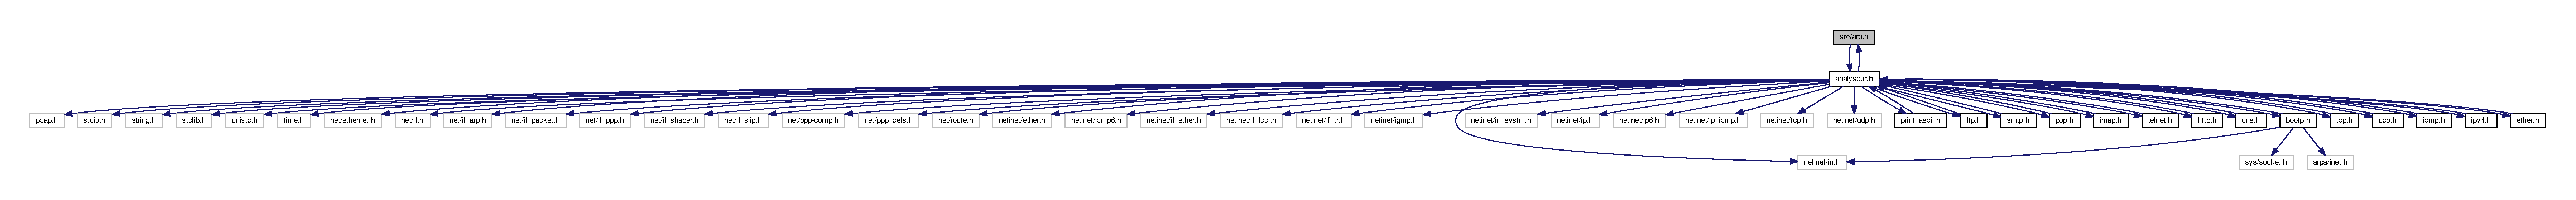
\includegraphics[width=350pt]{arp_8h__incl}
\end{center}
\end{figure}
This graph shows which files directly or indirectly include this file\+:
\nopagebreak
\begin{figure}[H]
\begin{center}
\leavevmode
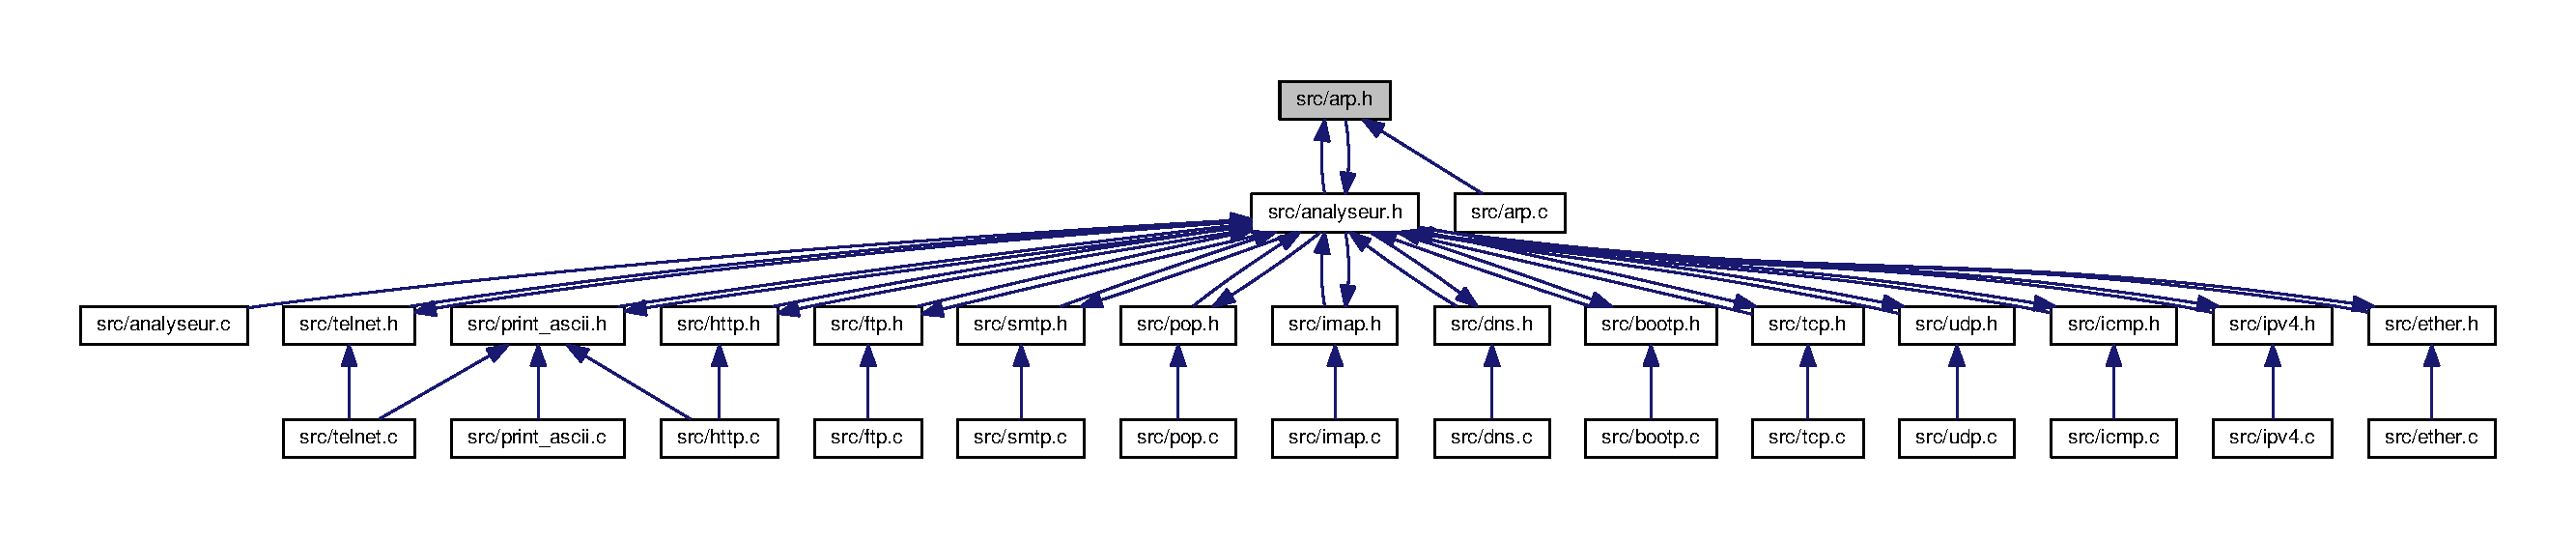
\includegraphics[width=350pt]{arp_8h__dep__incl}
\end{center}
\end{figure}
\subsection*{Functions}
\begin{DoxyCompactItemize}
\item 
void \hyperlink{arp_8h_af2c37cf12e56fd074bc1d35e46b9536f}{analyse\+\_\+arp} (\hyperlink{struct_user}{User} $\ast$user, const u\+\_\+char $\ast$bytes)
\end{DoxyCompactItemize}


\subsection{Function Documentation}
\index{arp.\+h@{arp.\+h}!analyse\+\_\+arp@{analyse\+\_\+arp}}
\index{analyse\+\_\+arp@{analyse\+\_\+arp}!arp.\+h@{arp.\+h}}
\subsubsection[{\texorpdfstring{analyse\+\_\+arp(\+User $\ast$user, const u\+\_\+char $\ast$bytes)}{analyse_arp(User *user, const u_char *bytes)}}]{\setlength{\rightskip}{0pt plus 5cm}void analyse\+\_\+arp (
\begin{DoxyParamCaption}
\item[{{\bf User} $\ast$}]{user, }
\item[{const u\+\_\+char $\ast$}]{bytes}
\end{DoxyParamCaption}
)}\hypertarget{arp_8h_af2c37cf12e56fd074bc1d35e46b9536f}{}\label{arp_8h_af2c37cf12e56fd074bc1d35e46b9536f}

\hypertarget{bootp_8c}{}\section{src/bootp.c File Reference}
\label{bootp_8c}\index{src/bootp.\+c@{src/bootp.\+c}}
{\ttfamily \#include \char`\"{}bootp.\+h\char`\"{}}\\*
Include dependency graph for bootp.\+c\+:
\nopagebreak
\begin{figure}[H]
\begin{center}
\leavevmode
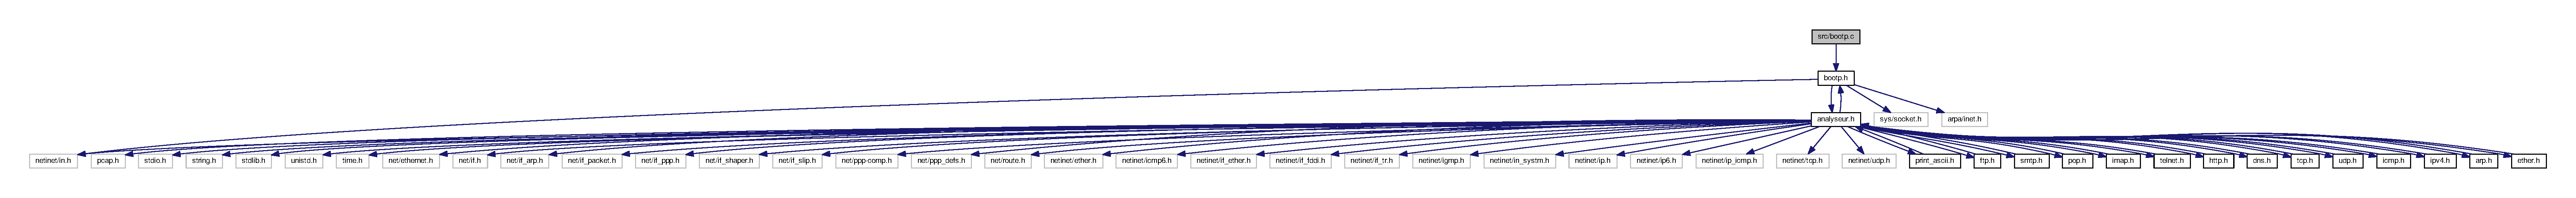
\includegraphics[width=350pt]{bootp_8c__incl}
\end{center}
\end{figure}
\subsection*{Functions}
\begin{DoxyCompactItemize}
\item 
void \hyperlink{bootp_8c_abfce5df4af834731a51ab00b6bcecf0a}{affichage\+\_\+bootp} (\hyperlink{struct_user}{User} $\ast$user, \hyperlink{analyseur_8h_abda6a1c8d85a6aab6c4819fe6e97c2d3}{Bootp} $\ast$\hyperlink{structbootp}{bootp}, const u\+\_\+char $\ast$bytes)
\begin{DoxyCompactList}\small\item\em Affiche les information sur le header. \end{DoxyCompactList}\item 
void \hyperlink{bootp_8c_a03223ad66d8f1d308590542731bd5269}{analyse\+\_\+bootp} (\hyperlink{struct_user}{User} $\ast$user, const u\+\_\+char $\ast$bytes)
\end{DoxyCompactItemize}


\subsection{Function Documentation}
\index{bootp.\+c@{bootp.\+c}!affichage\+\_\+bootp@{affichage\+\_\+bootp}}
\index{affichage\+\_\+bootp@{affichage\+\_\+bootp}!bootp.\+c@{bootp.\+c}}
\subsubsection[{\texorpdfstring{affichage\+\_\+bootp(\+User $\ast$user, Bootp $\ast$bootp, const u\+\_\+char $\ast$bytes)}{affichage_bootp(User *user, Bootp *bootp, const u_char *bytes)}}]{\setlength{\rightskip}{0pt plus 5cm}void affichage\+\_\+bootp (
\begin{DoxyParamCaption}
\item[{{\bf User} $\ast$}]{user, }
\item[{{\bf Bootp} $\ast$}]{bootp, }
\item[{const u\+\_\+char $\ast$}]{bytes}
\end{DoxyParamCaption}
)}\hypertarget{bootp_8c_abfce5df4af834731a51ab00b6bcecf0a}{}\label{bootp_8c_abfce5df4af834731a51ab00b6bcecf0a}


Affiche les information sur le header. 

Affichage en fonction de la verbosité


\begin{DoxyParams}{Parameters}
{\em user} & \\
\hline
{\em bootp} & \\
\hline
{\em bytes} & \\
\hline
\end{DoxyParams}
\index{bootp.\+c@{bootp.\+c}!analyse\+\_\+bootp@{analyse\+\_\+bootp}}
\index{analyse\+\_\+bootp@{analyse\+\_\+bootp}!bootp.\+c@{bootp.\+c}}
\subsubsection[{\texorpdfstring{analyse\+\_\+bootp(\+User $\ast$user, const u\+\_\+char $\ast$bytes)}{analyse_bootp(User *user, const u_char *bytes)}}]{\setlength{\rightskip}{0pt plus 5cm}void analyse\+\_\+bootp (
\begin{DoxyParamCaption}
\item[{{\bf User} $\ast$}]{user, }
\item[{const u\+\_\+char $\ast$}]{bytes}
\end{DoxyParamCaption}
)}\hypertarget{bootp_8c_a03223ad66d8f1d308590542731bd5269}{}\label{bootp_8c_a03223ad66d8f1d308590542731bd5269}

\hypertarget{bootp_8h}{}\section{src/bootp.h File Reference}
\label{bootp_8h}\index{src/bootp.\+h@{src/bootp.\+h}}
{\ttfamily \#include \char`\"{}analyseur.\+h\char`\"{}}\\*
{\ttfamily \#include $<$sys/socket.\+h$>$}\\*
{\ttfamily \#include $<$netinet/in.\+h$>$}\\*
{\ttfamily \#include $<$arpa/inet.\+h$>$}\\*
Include dependency graph for bootp.\+h\+:
\nopagebreak
\begin{figure}[H]
\begin{center}
\leavevmode
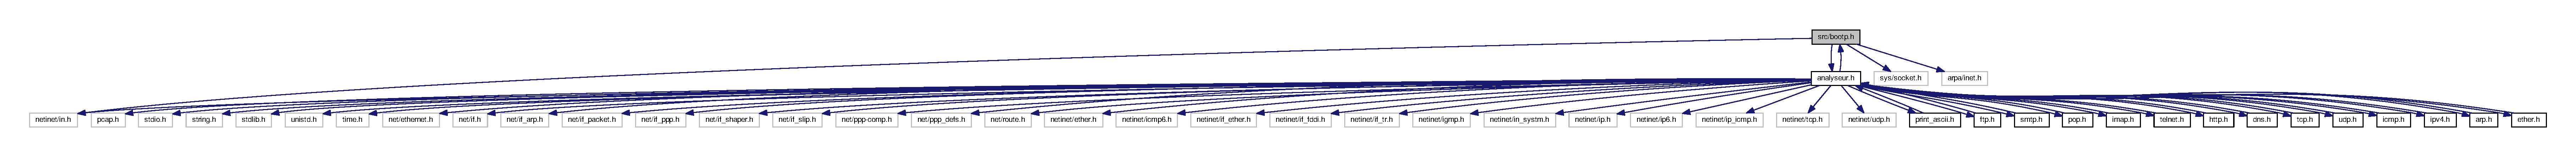
\includegraphics[width=350pt]{bootp_8h__incl}
\end{center}
\end{figure}
This graph shows which files directly or indirectly include this file\+:
\nopagebreak
\begin{figure}[H]
\begin{center}
\leavevmode
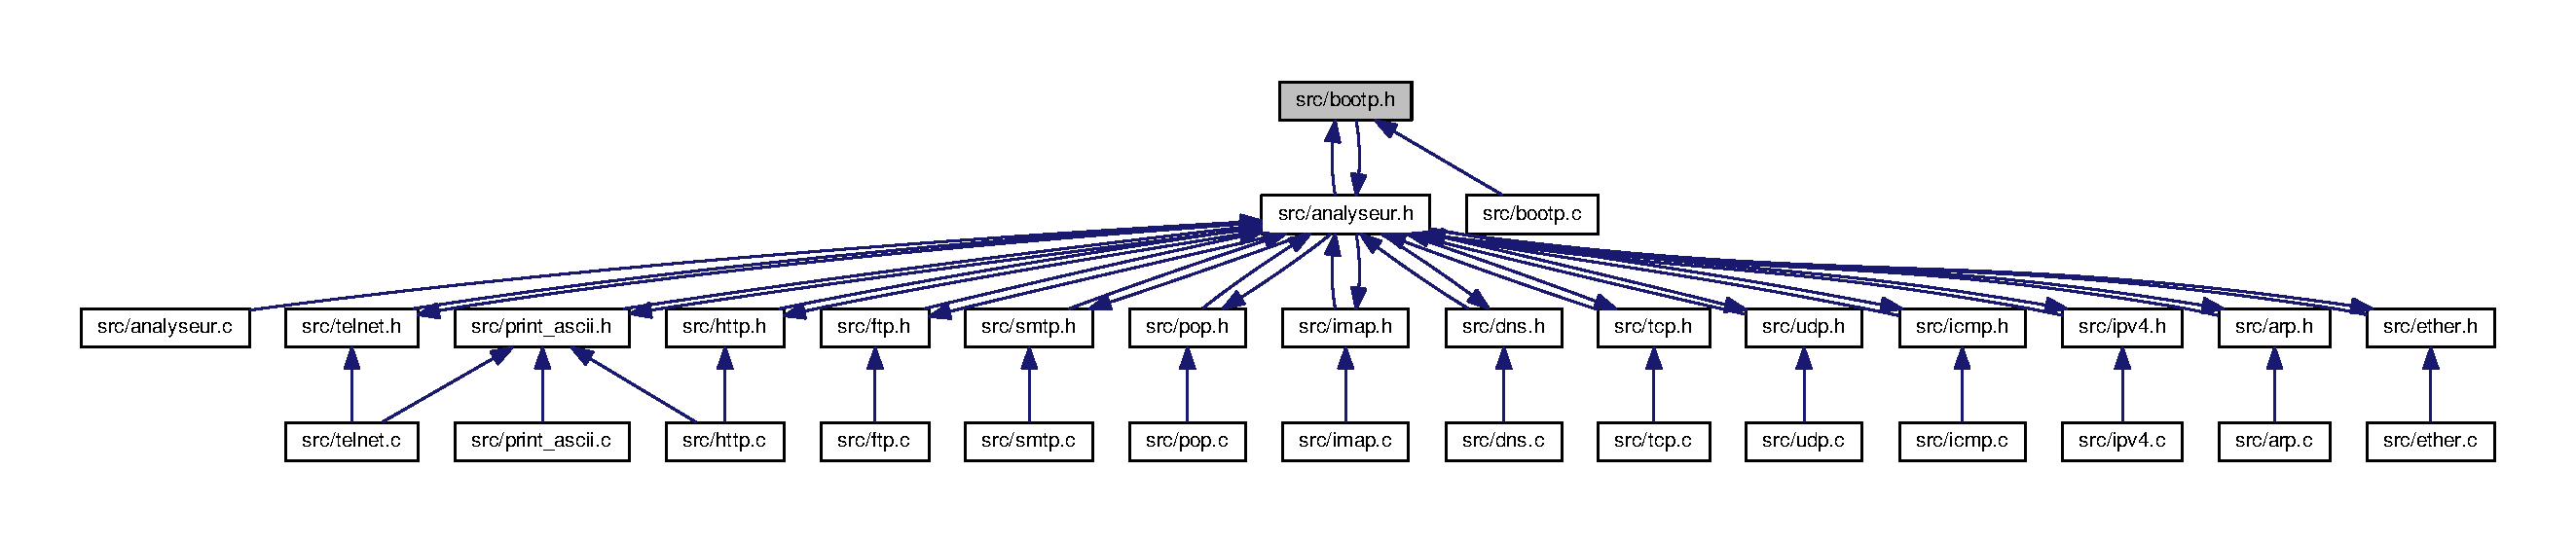
\includegraphics[width=350pt]{bootp_8h__dep__incl}
\end{center}
\end{figure}
\subsection*{Data Structures}
\begin{DoxyCompactItemize}
\item 
struct \hyperlink{structbootp}{bootp}
\item 
struct \hyperlink{structcmu__vend}{cmu\+\_\+vend}
\end{DoxyCompactItemize}
\subsection*{Macros}
\begin{DoxyCompactItemize}
\item 
\#define \hyperlink{bootp_8h_a70050ce8083e7150f7381f919dd2e925}{I\+P\+P\+O\+R\+T\+\_\+\+B\+O\+O\+T\+PS}~67
\item 
\#define \hyperlink{bootp_8h_af7a147a75769140ea18485e0b1b960d7}{I\+P\+P\+O\+R\+T\+\_\+\+B\+O\+O\+T\+PC}~68
\item 
\#define \hyperlink{bootp_8h_a5f62105e3377914bcecf431b331cf285}{B\+O\+O\+T\+R\+E\+P\+LY}~2
\item 
\#define \hyperlink{bootp_8h_aa43f2f422c8548259b3940122561c603}{B\+O\+O\+T\+R\+E\+Q\+U\+E\+ST}~1
\item 
\#define \hyperlink{bootp_8h_abddefef5916775b5acc20ee71aecef29}{V\+M\+\_\+\+C\+MU}~\char`\"{}C\+MU\char`\"{}
\item 
\#define \hyperlink{bootp_8h_a820b3fe666b520a70046dbd1e773ebf8}{V\+M\+\_\+\+R\+F\+C1048}~\{ 99, 130, 83, 99 \}
\item 
\#define \hyperlink{bootp_8h_aa33a6028e3d11c1ac472768218370e28}{T\+A\+G\+\_\+\+P\+AD}~((u\+\_\+int8\+\_\+t)   0)
\item 
\#define \hyperlink{bootp_8h_af45805e912a3be64afda28ea8e8eaeba}{T\+A\+G\+\_\+\+S\+U\+B\+N\+E\+T\+\_\+\+M\+A\+SK}~((u\+\_\+int8\+\_\+t)   1)
\item 
\#define \hyperlink{bootp_8h_a390f567e5538ba6ce98b5785737ac935}{T\+A\+G\+\_\+\+T\+I\+M\+E\+\_\+\+O\+F\+F\+S\+ET}~((u\+\_\+int8\+\_\+t)   2)
\item 
\#define \hyperlink{bootp_8h_a0c201387c95df4fb85ab70ad7462f982}{T\+A\+G\+\_\+\+G\+A\+T\+E\+W\+AY}~((u\+\_\+int8\+\_\+t)   3)
\item 
\#define \hyperlink{bootp_8h_af062a7f992d1429fa671944062daa347}{T\+A\+G\+\_\+\+T\+I\+M\+E\+\_\+\+S\+E\+R\+V\+ER}~((u\+\_\+int8\+\_\+t)   4)
\item 
\#define \hyperlink{bootp_8h_a1690a98a3bb603c701beb9db2984e9df}{T\+A\+G\+\_\+\+N\+A\+M\+E\+\_\+\+S\+E\+R\+V\+ER}~((u\+\_\+int8\+\_\+t)   5)
\item 
\#define \hyperlink{bootp_8h_a1a31de9732c87c8909107e260391548a}{T\+A\+G\+\_\+\+D\+O\+M\+A\+I\+N\+\_\+\+S\+E\+R\+V\+ER}~((u\+\_\+int8\+\_\+t)   6)
\item 
\#define \hyperlink{bootp_8h_a9e197f1ecede6f2dd6e6921349e6604c}{T\+A\+G\+\_\+\+L\+O\+G\+\_\+\+S\+E\+R\+V\+ER}~((u\+\_\+int8\+\_\+t)   7)
\item 
\#define \hyperlink{bootp_8h_a60f6f7bc6e3096ebda35264477475238}{T\+A\+G\+\_\+\+C\+O\+O\+K\+I\+E\+\_\+\+S\+E\+R\+V\+ER}~((u\+\_\+int8\+\_\+t)   8)
\item 
\#define \hyperlink{bootp_8h_aacca3eb5938baa3e46ed8153daebb2af}{T\+A\+G\+\_\+\+L\+P\+R\+\_\+\+S\+E\+R\+V\+ER}~((u\+\_\+int8\+\_\+t)   9)
\item 
\#define \hyperlink{bootp_8h_a6f0e4cbbf9f0c79f04eedac0962c89d4}{T\+A\+G\+\_\+\+I\+M\+P\+R\+E\+S\+S\+\_\+\+S\+E\+R\+V\+ER}~((u\+\_\+int8\+\_\+t)  10)
\item 
\#define \hyperlink{bootp_8h_ab3be008e5d6554d834417cd8535f6533}{T\+A\+G\+\_\+\+R\+L\+P\+\_\+\+S\+E\+R\+V\+ER}~((u\+\_\+int8\+\_\+t)  11)
\item 
\#define \hyperlink{bootp_8h_ae43c79d10663fa17ac1a60058eec8908}{T\+A\+G\+\_\+\+H\+O\+S\+T\+N\+A\+ME}~((u\+\_\+int8\+\_\+t)  12)
\item 
\#define \hyperlink{bootp_8h_a6454eb77897b265b54aa953384c8c892}{T\+A\+G\+\_\+\+B\+O\+O\+T\+S\+I\+ZE}~((u\+\_\+int8\+\_\+t)  13)
\item 
\#define \hyperlink{bootp_8h_a0f5b90506631a30c98593c247eab2005}{T\+A\+G\+\_\+\+E\+ND}~((u\+\_\+int8\+\_\+t) 255)
\item 
\#define \hyperlink{bootp_8h_abc384bc0b0c553ef87630dc015f8cca2}{T\+A\+G\+\_\+\+D\+U\+M\+P\+P\+A\+TH}~((u\+\_\+int8\+\_\+t)  14)
\item 
\#define \hyperlink{bootp_8h_ac5c3a05643edc3591809d25a88205ba4}{T\+A\+G\+\_\+\+D\+O\+M\+A\+I\+N\+N\+A\+ME}~((u\+\_\+int8\+\_\+t)  15)
\item 
\#define \hyperlink{bootp_8h_a249cc427fd7c2e9a81fb68a85131804a}{T\+A\+G\+\_\+\+S\+W\+A\+P\+\_\+\+S\+E\+R\+V\+ER}~((u\+\_\+int8\+\_\+t)  16)
\item 
\#define \hyperlink{bootp_8h_a55bce3580e9b40eee751b5b08f2dd623}{T\+A\+G\+\_\+\+R\+O\+O\+T\+P\+A\+TH}~((u\+\_\+int8\+\_\+t)  17)
\item 
\#define \hyperlink{bootp_8h_a0624a616b1083292cb667d16fe10abe2}{T\+A\+G\+\_\+\+E\+X\+T\+P\+A\+TH}~((u\+\_\+int8\+\_\+t)  18)
\item 
\#define \hyperlink{bootp_8h_a7d8a3445f9b72e9cac32e25b11576c5c}{T\+A\+G\+\_\+\+I\+P\+\_\+\+F\+O\+R\+W\+A\+RD}~((u\+\_\+int8\+\_\+t)  19)
\item 
\#define \hyperlink{bootp_8h_a71e186b9d7a70c2d7679788bd928dc13}{T\+A\+G\+\_\+\+N\+L\+\_\+\+S\+R\+C\+RT}~((u\+\_\+int8\+\_\+t)  20)
\item 
\#define \hyperlink{bootp_8h_adcca9220a2624dbb363da76eba5f6f4d}{T\+A\+G\+\_\+\+P\+F\+I\+L\+T\+E\+RS}~((u\+\_\+int8\+\_\+t)  21)
\item 
\#define \hyperlink{bootp_8h_a05c21b9082e83efa2699a4506cbea6bd}{T\+A\+G\+\_\+\+R\+E\+A\+S\+S\+\_\+\+S\+I\+ZE}~((u\+\_\+int8\+\_\+t)  22)
\item 
\#define \hyperlink{bootp_8h_ae3514ce26955b52ec801f6874ef3daf1}{T\+A\+G\+\_\+\+D\+E\+F\+\_\+\+T\+TL}~((u\+\_\+int8\+\_\+t)  23)
\item 
\#define \hyperlink{bootp_8h_a733b27220789644b16ef7d6772620454}{T\+A\+G\+\_\+\+M\+T\+U\+\_\+\+T\+I\+M\+E\+O\+UT}~((u\+\_\+int8\+\_\+t)  24)
\item 
\#define \hyperlink{bootp_8h_a36a96a5f60c7b1392bdbe408b51a8a3b}{T\+A\+G\+\_\+\+M\+T\+U\+\_\+\+T\+A\+B\+LE}~((u\+\_\+int8\+\_\+t)  25)
\item 
\#define \hyperlink{bootp_8h_a8ad5067b5876f23506bfce58891c99e2}{T\+A\+G\+\_\+\+I\+N\+T\+\_\+\+M\+TU}~((u\+\_\+int8\+\_\+t)  26)
\item 
\#define \hyperlink{bootp_8h_ac740e8a45d17b0bd1e36e9dc048c7cf0}{T\+A\+G\+\_\+\+L\+O\+C\+A\+L\+\_\+\+S\+U\+B\+N\+E\+TS}~((u\+\_\+int8\+\_\+t)  27)
\item 
\#define \hyperlink{bootp_8h_aad64c0c192f2ccc65757c513828df6e2}{T\+A\+G\+\_\+\+B\+R\+O\+A\+D\+\_\+\+A\+D\+DR}~((u\+\_\+int8\+\_\+t)  28)
\item 
\#define \hyperlink{bootp_8h_a49b1768b4c6ff9849ccfd27398075bba}{T\+A\+G\+\_\+\+D\+O\+\_\+\+M\+A\+S\+K\+\_\+\+D\+I\+SC}~((u\+\_\+int8\+\_\+t)  29)
\item 
\#define \hyperlink{bootp_8h_a4c62966ac63fe3c31e584b67fa0836d6}{T\+A\+G\+\_\+\+S\+U\+P\+P\+L\+Y\+\_\+\+M\+A\+SK}~((u\+\_\+int8\+\_\+t)  30)
\item 
\#define \hyperlink{bootp_8h_af5c84aa233527d852c9788fc7604bcf0}{T\+A\+G\+\_\+\+D\+O\+\_\+\+R\+D\+I\+SC}~((u\+\_\+int8\+\_\+t)  31)
\item 
\#define \hyperlink{bootp_8h_a8def057d40c83dd9956e30415758cf90}{T\+A\+G\+\_\+\+R\+T\+R\+\_\+\+S\+O\+L\+\_\+\+A\+D\+DR}~((u\+\_\+int8\+\_\+t)  32)
\item 
\#define \hyperlink{bootp_8h_a323cc9c0eb9283ee1c82c002f4640543}{T\+A\+G\+\_\+\+S\+T\+A\+T\+I\+C\+\_\+\+R\+O\+U\+TE}~((u\+\_\+int8\+\_\+t)  33)
\item 
\#define \hyperlink{bootp_8h_af36210ca451c38c20a4f92c986c42a31}{T\+A\+G\+\_\+\+U\+S\+E\+\_\+\+T\+R\+A\+I\+L\+E\+RS}~((u\+\_\+int8\+\_\+t)  34)
\item 
\#define \hyperlink{bootp_8h_aa0b827fe249fe68705893ac2e1f26d6d}{T\+A\+G\+\_\+\+A\+R\+P\+\_\+\+T\+I\+M\+E\+O\+UT}~((u\+\_\+int8\+\_\+t)  35)
\item 
\#define \hyperlink{bootp_8h_af4099985b9fee6dddf6260ded7b1b6ad}{T\+A\+G\+\_\+\+E\+T\+H\+\_\+\+E\+N\+C\+AP}~((u\+\_\+int8\+\_\+t)  36)
\item 
\#define \hyperlink{bootp_8h_a7f5879d8eb0f730f1ed3118b0e9c9e2f}{T\+A\+G\+\_\+\+T\+C\+P\+\_\+\+T\+TL}~((u\+\_\+int8\+\_\+t)  37)
\item 
\#define \hyperlink{bootp_8h_aed45b20de1ad6ee9bd75ff205c92f62d}{T\+A\+G\+\_\+\+T\+C\+P\+\_\+\+K\+E\+E\+P\+A\+L\+I\+VE}~((u\+\_\+int8\+\_\+t)  38)
\item 
\#define \hyperlink{bootp_8h_a40d0f27091c427a5d4ab5450510d85fa}{T\+A\+G\+\_\+\+K\+E\+E\+P\+A\+L\+I\+V\+E\+\_\+\+GO}~((u\+\_\+int8\+\_\+t)  39)
\item 
\#define \hyperlink{bootp_8h_a1888cc12d68ff72abaf9522b46fe2a79}{T\+A\+G\+\_\+\+N\+I\+S\+\_\+\+D\+O\+M\+A\+IN}~((u\+\_\+int8\+\_\+t)  40)
\item 
\#define \hyperlink{bootp_8h_a6be57dc426b9ce8279fe4207a7689908}{T\+A\+G\+\_\+\+N\+I\+S\+\_\+\+S\+E\+R\+V\+E\+RS}~((u\+\_\+int8\+\_\+t)  41)
\item 
\#define \hyperlink{bootp_8h_a477501e5b93d3c0f425f13dcf59b3e9f}{T\+A\+G\+\_\+\+N\+T\+P\+\_\+\+S\+E\+R\+V\+E\+RS}~((u\+\_\+int8\+\_\+t)  42)
\item 
\#define \hyperlink{bootp_8h_aa328232fe4481e07d370a0490644a387}{T\+A\+G\+\_\+\+V\+E\+N\+D\+O\+R\+\_\+\+O\+P\+TS}~((u\+\_\+int8\+\_\+t)  43)
\item 
\#define \hyperlink{bootp_8h_ad1eb7881db3ab55b75a98ee7241866ad}{T\+A\+G\+\_\+\+N\+E\+T\+B\+I\+O\+S\+\_\+\+NS}~((u\+\_\+int8\+\_\+t)  44)
\item 
\#define \hyperlink{bootp_8h_adc0ebd710a9d77d9f0d346630c3301b3}{T\+A\+G\+\_\+\+N\+E\+T\+B\+I\+O\+S\+\_\+\+D\+DS}~((u\+\_\+int8\+\_\+t)  45)
\item 
\#define \hyperlink{bootp_8h_a616d16e18c5e16f26697d6620c36f3cd}{T\+A\+G\+\_\+\+N\+E\+T\+B\+I\+O\+S\+\_\+\+N\+O\+DE}~((u\+\_\+int8\+\_\+t)  46)
\item 
\#define \hyperlink{bootp_8h_ac3dbdb16312f0af69e1383841fdff801}{T\+A\+G\+\_\+\+N\+E\+T\+B\+I\+O\+S\+\_\+\+S\+C\+O\+PE}~((u\+\_\+int8\+\_\+t)  47)
\item 
\#define \hyperlink{bootp_8h_a3da8f45962f618598d64079e65f76fa4}{T\+A\+G\+\_\+\+X\+W\+I\+N\+\_\+\+FS}~((u\+\_\+int8\+\_\+t)  48)
\item 
\#define \hyperlink{bootp_8h_a92ef7e83aaee277d79fdb787f4725ac6}{T\+A\+G\+\_\+\+X\+W\+I\+N\+\_\+\+DM}~((u\+\_\+int8\+\_\+t)  49)
\item 
\#define \hyperlink{bootp_8h_a0d453c2c2e58ac10b0cc16010121c1ec}{T\+A\+G\+\_\+\+N\+I\+S\+\_\+\+P\+\_\+\+D\+O\+M\+A\+IN}~((u\+\_\+int8\+\_\+t)  64)
\item 
\#define \hyperlink{bootp_8h_a1b3a212a9794022dbd6718e0bbf84c02}{T\+A\+G\+\_\+\+N\+I\+S\+\_\+\+P\+\_\+\+S\+E\+R\+V\+E\+RS}~((u\+\_\+int8\+\_\+t)  65)
\item 
\#define \hyperlink{bootp_8h_a567249432977821d54de8f9726098d02}{T\+A\+G\+\_\+\+M\+O\+B\+I\+L\+E\+\_\+\+H\+O\+ME}~((u\+\_\+int8\+\_\+t)  68)
\item 
\#define \hyperlink{bootp_8h_af8fe6f270c2a34fcc8c835cf1f717aff}{T\+A\+G\+\_\+\+S\+M\+P\+T\+\_\+\+S\+E\+R\+V\+ER}~((u\+\_\+int8\+\_\+t)  69)
\item 
\#define \hyperlink{bootp_8h_a75a4fa97ae81fcfe141f4d80631012b7}{T\+A\+G\+\_\+\+P\+O\+P3\+\_\+\+S\+E\+R\+V\+ER}~((u\+\_\+int8\+\_\+t)  70)
\item 
\#define \hyperlink{bootp_8h_ac0337d37b9410d9e0f18a2c67150534c}{T\+A\+G\+\_\+\+N\+N\+T\+P\+\_\+\+S\+E\+R\+V\+ER}~((u\+\_\+int8\+\_\+t)  71)
\item 
\#define \hyperlink{bootp_8h_a26422c2dd83e344e56a56c43eab83ebc}{T\+A\+G\+\_\+\+W\+W\+W\+\_\+\+S\+E\+R\+V\+ER}~((u\+\_\+int8\+\_\+t)  72)
\item 
\#define \hyperlink{bootp_8h_a0b91191d204431df9db1f0a122313340}{T\+A\+G\+\_\+\+F\+I\+N\+G\+E\+R\+\_\+\+S\+E\+R\+V\+ER}~((u\+\_\+int8\+\_\+t)  73)
\item 
\#define \hyperlink{bootp_8h_a76da3a16f1ef23e1d4cc1c0ee4abae10}{T\+A\+G\+\_\+\+I\+R\+C\+\_\+\+S\+E\+R\+V\+ER}~((u\+\_\+int8\+\_\+t)  74)
\item 
\#define \hyperlink{bootp_8h_a1bd3e74bcb159b3b5eb0213222909847}{T\+A\+G\+\_\+\+S\+T\+R\+E\+E\+T\+T\+A\+L\+K\+\_\+\+S\+R\+VR}~((u\+\_\+int8\+\_\+t)  75)
\item 
\#define \hyperlink{bootp_8h_a5ffbdc8df4b0234ef7fa542ee8366e0f}{T\+A\+G\+\_\+\+S\+T\+R\+E\+E\+T\+T\+A\+L\+K\+\_\+\+S\+T\+DA}~((u\+\_\+int8\+\_\+t)  76)
\item 
\#define \hyperlink{bootp_8h_a8606f39a5eff6f5ba7fdd1b92c2b1858}{T\+A\+G\+\_\+\+R\+E\+Q\+U\+E\+S\+T\+E\+D\+\_\+\+IP}~((u\+\_\+int8\+\_\+t)  50)
\item 
\#define \hyperlink{bootp_8h_a73359f0f42ab3a399356c7f42aa4a272}{T\+A\+G\+\_\+\+I\+P\+\_\+\+L\+E\+A\+SE}~((u\+\_\+int8\+\_\+t)  51)
\item 
\#define \hyperlink{bootp_8h_a422cc1829a1484432030af4d77486953}{T\+A\+G\+\_\+\+O\+P\+T\+\_\+\+O\+V\+E\+R\+L\+O\+AD}~((u\+\_\+int8\+\_\+t)  52)
\item 
\#define \hyperlink{bootp_8h_afec90448cf3385df7ff611d327a03273}{T\+A\+G\+\_\+\+T\+F\+T\+P\+\_\+\+S\+E\+R\+V\+ER}~((u\+\_\+int8\+\_\+t)  66)
\item 
\#define \hyperlink{bootp_8h_afeb74f0db83aac8e50b5dbd02ee82230}{T\+A\+G\+\_\+\+B\+O\+O\+T\+F\+I\+L\+E\+N\+A\+ME}~((u\+\_\+int8\+\_\+t)  67)
\item 
\#define \hyperlink{bootp_8h_a2352657fb0071a03e456e3b1c769c05f}{T\+A\+G\+\_\+\+D\+H\+C\+P\+\_\+\+M\+E\+S\+S\+A\+GE}~((u\+\_\+int8\+\_\+t)  53)
\item 
\#define \hyperlink{bootp_8h_ae7424e0dbbb32b09a83e888f172d20d9}{T\+A\+G\+\_\+\+S\+E\+R\+V\+E\+R\+\_\+\+ID}~((u\+\_\+int8\+\_\+t)  54)
\item 
\#define \hyperlink{bootp_8h_a3c25d0b0f2c989317a72ba7fba0f8b84}{T\+A\+G\+\_\+\+P\+A\+R\+M\+\_\+\+R\+E\+Q\+U\+E\+ST}~((u\+\_\+int8\+\_\+t)  55)
\item 
\#define \hyperlink{bootp_8h_a6c91d1804f4053993dc463fbc9708d70}{T\+A\+G\+\_\+\+M\+E\+S\+S\+A\+GE}~((u\+\_\+int8\+\_\+t)  56)
\item 
\#define \hyperlink{bootp_8h_a242f2e9c5dbc669438f744ea1d56be28}{T\+A\+G\+\_\+\+M\+A\+X\+\_\+\+M\+S\+G\+\_\+\+S\+I\+ZE}~((u\+\_\+int8\+\_\+t)  57)
\item 
\#define \hyperlink{bootp_8h_a4bd3db9994ad434b399ee57282ff9adf}{T\+A\+G\+\_\+\+R\+E\+N\+E\+W\+A\+L\+\_\+\+T\+I\+ME}~((u\+\_\+int8\+\_\+t)  58)
\item 
\#define \hyperlink{bootp_8h_ae4902632ad26317fc82557955b6e0708}{T\+A\+G\+\_\+\+R\+E\+B\+I\+N\+D\+\_\+\+T\+I\+ME}~((u\+\_\+int8\+\_\+t)  59)
\item 
\#define \hyperlink{bootp_8h_a041f49389806fdb350857b7b9a79df64}{T\+A\+G\+\_\+\+V\+E\+N\+D\+O\+R\+\_\+\+C\+L\+A\+SS}~((u\+\_\+int8\+\_\+t)  60)
\item 
\#define \hyperlink{bootp_8h_a3472ed610e7decb785ff5afcfb234124}{T\+A\+G\+\_\+\+C\+L\+I\+E\+N\+T\+\_\+\+ID}~((u\+\_\+int8\+\_\+t)  61)
\item 
\#define \hyperlink{bootp_8h_ac54c27f7628eb8258423a0f0a773cced}{T\+A\+G\+\_\+\+N\+D\+S\+\_\+\+S\+E\+R\+V\+E\+RS}~((u\+\_\+int8\+\_\+t)  85)
\item 
\#define \hyperlink{bootp_8h_aa78e08154a516a79de65ed56f4c8efdf}{T\+A\+G\+\_\+\+N\+D\+S\+\_\+\+T\+R\+E\+E\+\_\+\+N\+A\+ME}~((u\+\_\+int8\+\_\+t)  86)
\item 
\#define \hyperlink{bootp_8h_ac5d5a4cf3146d7cfeb884d5b4126e427}{T\+A\+G\+\_\+\+N\+D\+S\+\_\+\+C\+O\+N\+T\+E\+XT}~((u\+\_\+int8\+\_\+t)  87)
\item 
\#define \hyperlink{bootp_8h_a6861d790875e56adacccf8dbca8cffad}{T\+A\+G\+\_\+\+N\+D\+S\+\_\+\+I\+P\+D\+O\+M\+A\+IN}~((u\+\_\+int8\+\_\+t)  62)
\item 
\#define \hyperlink{bootp_8h_af399e70c5dcd85989d20ba4a4c8a5af9}{T\+A\+G\+\_\+\+N\+D\+S\+\_\+\+I\+P\+I\+N\+FO}~((u\+\_\+int8\+\_\+t)  63)
\item 
\#define \hyperlink{bootp_8h_aae19e9ec17d3370fcb7a6eaa6f51734a}{T\+A\+G\+\_\+\+O\+P\+E\+N\+\_\+\+G\+R\+O\+U\+P\+\_\+\+U\+AP}~((u\+\_\+int8\+\_\+t)  98)
\item 
\#define \hyperlink{bootp_8h_a2fddae87b7fec5934f425932664bb337}{T\+A\+G\+\_\+\+D\+I\+S\+A\+B\+L\+E\+\_\+\+A\+U\+T\+O\+C\+O\+NF}~((u\+\_\+int8\+\_\+t) 116)
\item 
\#define \hyperlink{bootp_8h_a769e5c292796170e5c4a0339ff55de9d}{T\+A\+G\+\_\+\+S\+L\+P\+\_\+\+DA}~((u\+\_\+int8\+\_\+t)  78)
\item 
\#define \hyperlink{bootp_8h_a51cebf6450d79e206db6a2c6e2be7c69}{T\+A\+G\+\_\+\+S\+L\+P\+\_\+\+S\+C\+O\+PE}~((u\+\_\+int8\+\_\+t)  79)
\item 
\#define \hyperlink{bootp_8h_ac3dca2fe75dc1eeb0e12353801a7a8d5}{T\+A\+G\+\_\+\+N\+S\+\_\+\+S\+E\+A\+R\+CH}~((u\+\_\+int8\+\_\+t) 117)
\item 
\#define \hyperlink{bootp_8h_a5665b2c3417c826a98d540029d4d0407}{T\+A\+G\+\_\+\+I\+P4\+\_\+\+S\+U\+B\+N\+E\+T\+\_\+\+S\+E\+L\+E\+CT}~((u\+\_\+int8\+\_\+t) 118)
\item 
\#define \hyperlink{bootp_8h_a1dec6db39d17aac5dcd34edd36eb3552}{T\+A\+G\+\_\+\+U\+S\+E\+R\+\_\+\+C\+L\+A\+SS}~((u\+\_\+int8\+\_\+t)  77)
\item 
\#define \hyperlink{bootp_8h_aea609e62cf58fed0165e9baec03a9712}{T\+A\+G\+\_\+\+S\+L\+P\+\_\+\+N\+A\+M\+I\+N\+G\+\_\+\+A\+U\+TH}~((u\+\_\+int8\+\_\+t)  80)
\item 
\#define \hyperlink{bootp_8h_a6c8671954650acc12846013c938048e2}{T\+A\+G\+\_\+\+C\+L\+I\+E\+N\+T\+\_\+\+F\+Q\+DN}~((u\+\_\+int8\+\_\+t)  81)
\item 
\#define \hyperlink{bootp_8h_a54d0f83bf53808d53e539e98f58b9565}{T\+A\+G\+\_\+\+A\+G\+E\+N\+T\+\_\+\+C\+I\+R\+C\+U\+IT}~((u\+\_\+int8\+\_\+t)  82)
\item 
\#define \hyperlink{bootp_8h_a4dddfdb523a41a2b9011ebf9638f656b}{T\+A\+G\+\_\+\+A\+G\+E\+N\+T\+\_\+\+R\+E\+M\+O\+TE}~((u\+\_\+int8\+\_\+t)  83)
\item 
\#define \hyperlink{bootp_8h_af179e22b8ecaf3b3645d6b343a57df61}{T\+A\+G\+\_\+\+A\+G\+E\+N\+T\+\_\+\+M\+A\+SK}~((u\+\_\+int8\+\_\+t)  84)
\item 
\#define \hyperlink{bootp_8h_a9c3ecc0aa3a3c0adec3ff88e5b59d640}{T\+A\+G\+\_\+\+T\+Z\+\_\+\+S\+T\+R\+I\+NG}~((u\+\_\+int8\+\_\+t)  88)
\item 
\#define \hyperlink{bootp_8h_a3b165888715df26722794882a693240e}{T\+A\+G\+\_\+\+F\+Q\+D\+N\+\_\+\+O\+P\+T\+I\+ON}~((u\+\_\+int8\+\_\+t)  89)
\item 
\#define \hyperlink{bootp_8h_a8c8970730d9fa54fe582b142f301d7a3}{T\+A\+G\+\_\+\+A\+U\+TH}~((u\+\_\+int8\+\_\+t)  90)
\item 
\#define \hyperlink{bootp_8h_ae003122a7e522a04d5b81d0ec42b0658}{T\+A\+G\+\_\+\+V\+I\+N\+E\+S\+\_\+\+S\+E\+R\+V\+E\+RS}~((u\+\_\+int8\+\_\+t)  91)
\item 
\#define \hyperlink{bootp_8h_a586e958f26cc0aae12226a16f60c99ac}{T\+A\+G\+\_\+\+S\+E\+R\+V\+E\+R\+\_\+\+R\+A\+NK}~((u\+\_\+int8\+\_\+t)  92)
\item 
\#define \hyperlink{bootp_8h_acb35ccf573f0c90cdbe42d5da2755493}{T\+A\+G\+\_\+\+C\+L\+I\+E\+N\+T\+\_\+\+A\+R\+CH}~((u\+\_\+int8\+\_\+t)  93)
\item 
\#define \hyperlink{bootp_8h_a0c64c1a88c5947e343701a4772a25bf7}{T\+A\+G\+\_\+\+C\+L\+I\+E\+N\+T\+\_\+\+N\+DI}~((u\+\_\+int8\+\_\+t)  94)
\item 
\#define \hyperlink{bootp_8h_a5a50de3c61b395af5e7bf69ec57a2f49}{T\+A\+G\+\_\+\+C\+L\+I\+E\+N\+T\+\_\+\+G\+U\+ID}~((u\+\_\+int8\+\_\+t)  97)
\item 
\#define \hyperlink{bootp_8h_af7ccb1922848af9c48b82d7368da0904}{T\+A\+G\+\_\+\+L\+D\+A\+P\+\_\+\+U\+RL}~((u\+\_\+int8\+\_\+t)  95)
\item 
\#define \hyperlink{bootp_8h_a5cbddeed52e84c82c701e0444d6d1d9c}{T\+A\+G\+\_\+6\+O\+V\+E\+R4}~((u\+\_\+int8\+\_\+t)  96)
\item 
\#define \hyperlink{bootp_8h_aa2104c4903a1116d8a439e8fbc7e13d2}{T\+A\+G\+\_\+\+P\+R\+I\+N\+T\+E\+R\+\_\+\+N\+A\+ME}~((u\+\_\+int8\+\_\+t) 100)
\item 
\#define \hyperlink{bootp_8h_a5c77c13c05a5c92aafe77043e3b08d8c}{T\+A\+G\+\_\+\+M\+D\+H\+C\+P\+\_\+\+S\+E\+R\+V\+ER}~((u\+\_\+int8\+\_\+t) 101)
\item 
\#define \hyperlink{bootp_8h_a0941b47b42e131e61c24bb14d3c513f7}{T\+A\+G\+\_\+\+I\+P\+X\+\_\+\+C\+O\+M\+P\+AT}~((u\+\_\+int8\+\_\+t) 110)
\item 
\#define \hyperlink{bootp_8h_ad5608dcafdceea1b46a419abbf73f602}{T\+A\+G\+\_\+\+N\+E\+T\+I\+N\+F\+O\+\_\+\+P\+A\+R\+E\+NT}~((u\+\_\+int8\+\_\+t) 112)
\item 
\#define \hyperlink{bootp_8h_a44afc205100b06bb8885eb6ace0b0e17}{T\+A\+G\+\_\+\+N\+E\+T\+I\+N\+F\+O\+\_\+\+P\+A\+R\+E\+N\+T\+\_\+\+T\+AG}~((u\+\_\+int8\+\_\+t) 113)
\item 
\#define \hyperlink{bootp_8h_ad2c8fb123db964e4b140ed7644db2337}{T\+A\+G\+\_\+\+U\+RL}~((u\+\_\+int8\+\_\+t) 114)
\item 
\#define \hyperlink{bootp_8h_a44459d01aedf556db9c8824c5ecdba57}{T\+A\+G\+\_\+\+F\+A\+I\+L\+O\+V\+ER}~((u\+\_\+int8\+\_\+t) 115)
\item 
\#define \hyperlink{bootp_8h_ac643a628fb0316ef7efc69f3e612bd47}{T\+A\+G\+\_\+\+E\+X\+T\+E\+N\+D\+E\+D\+\_\+\+R\+E\+Q\+U\+E\+ST}~((u\+\_\+int8\+\_\+t) 126)
\item 
\#define \hyperlink{bootp_8h_ac9e28170f08fc1099dcafaa928b217be}{T\+A\+G\+\_\+\+E\+X\+T\+E\+N\+D\+E\+D\+\_\+\+O\+P\+T\+I\+ON}~((u\+\_\+int8\+\_\+t) 127)
\item 
\#define \hyperlink{bootp_8h_aa490e80da21dfc13b91c034095efdcd4}{D\+H\+C\+P\+D\+I\+S\+C\+O\+V\+ER}~1
\item 
\#define \hyperlink{bootp_8h_ab82126d739f61a60d84116e1e0d3ad2e}{D\+H\+C\+P\+O\+F\+F\+ER}~2
\item 
\#define \hyperlink{bootp_8h_a0cd47b14d8040e76932488eadbc0091e}{D\+H\+C\+P\+R\+E\+Q\+U\+E\+ST}~3
\item 
\#define \hyperlink{bootp_8h_af03ae973e2eb857947af829f3611eed3}{D\+H\+C\+P\+D\+E\+C\+L\+I\+NE}~4
\item 
\#define \hyperlink{bootp_8h_a4f4105ef611737b700a6da965306dcfe}{D\+H\+C\+P\+A\+CK}~5
\item 
\#define \hyperlink{bootp_8h_a4162aa47e0c49f981f31b4bd0363476b}{D\+H\+C\+P\+N\+AK}~6
\item 
\#define \hyperlink{bootp_8h_a28d24149d2c3838966cc9f5cf2fdf2cb}{D\+H\+C\+P\+R\+E\+L\+E\+A\+SE}~7
\item 
\#define \hyperlink{bootp_8h_abb01731f0711308ff1e3f394da00d7c9}{D\+H\+C\+P\+I\+N\+F\+O\+RM}~8
\item 
\#define \hyperlink{bootp_8h_afa082c1dc543196c05eef42d7b0ef6e9}{V\+F\+\_\+\+S\+M\+A\+SK}~1	/$\ast$ Subnet mask field contains valid data $\ast$/
\end{DoxyCompactItemize}
\subsection*{Functions}
\begin{DoxyCompactItemize}
\item 
void \hyperlink{bootp_8h_a03223ad66d8f1d308590542731bd5269}{analyse\+\_\+bootp} (\hyperlink{struct_user}{User} $\ast$user, const u\+\_\+char $\ast$bytes)
\end{DoxyCompactItemize}


\subsection{Macro Definition Documentation}
\index{bootp.\+h@{bootp.\+h}!B\+O\+O\+T\+R\+E\+P\+LY@{B\+O\+O\+T\+R\+E\+P\+LY}}
\index{B\+O\+O\+T\+R\+E\+P\+LY@{B\+O\+O\+T\+R\+E\+P\+LY}!bootp.\+h@{bootp.\+h}}
\subsubsection[{\texorpdfstring{B\+O\+O\+T\+R\+E\+P\+LY}{BOOTREPLY}}]{\setlength{\rightskip}{0pt plus 5cm}\#define B\+O\+O\+T\+R\+E\+P\+LY~2}\hypertarget{bootp_8h_a5f62105e3377914bcecf431b331cf285}{}\label{bootp_8h_a5f62105e3377914bcecf431b331cf285}
\index{bootp.\+h@{bootp.\+h}!B\+O\+O\+T\+R\+E\+Q\+U\+E\+ST@{B\+O\+O\+T\+R\+E\+Q\+U\+E\+ST}}
\index{B\+O\+O\+T\+R\+E\+Q\+U\+E\+ST@{B\+O\+O\+T\+R\+E\+Q\+U\+E\+ST}!bootp.\+h@{bootp.\+h}}
\subsubsection[{\texorpdfstring{B\+O\+O\+T\+R\+E\+Q\+U\+E\+ST}{BOOTREQUEST}}]{\setlength{\rightskip}{0pt plus 5cm}\#define B\+O\+O\+T\+R\+E\+Q\+U\+E\+ST~1}\hypertarget{bootp_8h_aa43f2f422c8548259b3940122561c603}{}\label{bootp_8h_aa43f2f422c8548259b3940122561c603}
\index{bootp.\+h@{bootp.\+h}!D\+H\+C\+P\+A\+CK@{D\+H\+C\+P\+A\+CK}}
\index{D\+H\+C\+P\+A\+CK@{D\+H\+C\+P\+A\+CK}!bootp.\+h@{bootp.\+h}}
\subsubsection[{\texorpdfstring{D\+H\+C\+P\+A\+CK}{DHCPACK}}]{\setlength{\rightskip}{0pt plus 5cm}\#define D\+H\+C\+P\+A\+CK~5}\hypertarget{bootp_8h_a4f4105ef611737b700a6da965306dcfe}{}\label{bootp_8h_a4f4105ef611737b700a6da965306dcfe}
\index{bootp.\+h@{bootp.\+h}!D\+H\+C\+P\+D\+E\+C\+L\+I\+NE@{D\+H\+C\+P\+D\+E\+C\+L\+I\+NE}}
\index{D\+H\+C\+P\+D\+E\+C\+L\+I\+NE@{D\+H\+C\+P\+D\+E\+C\+L\+I\+NE}!bootp.\+h@{bootp.\+h}}
\subsubsection[{\texorpdfstring{D\+H\+C\+P\+D\+E\+C\+L\+I\+NE}{DHCPDECLINE}}]{\setlength{\rightskip}{0pt plus 5cm}\#define D\+H\+C\+P\+D\+E\+C\+L\+I\+NE~4}\hypertarget{bootp_8h_af03ae973e2eb857947af829f3611eed3}{}\label{bootp_8h_af03ae973e2eb857947af829f3611eed3}
\index{bootp.\+h@{bootp.\+h}!D\+H\+C\+P\+D\+I\+S\+C\+O\+V\+ER@{D\+H\+C\+P\+D\+I\+S\+C\+O\+V\+ER}}
\index{D\+H\+C\+P\+D\+I\+S\+C\+O\+V\+ER@{D\+H\+C\+P\+D\+I\+S\+C\+O\+V\+ER}!bootp.\+h@{bootp.\+h}}
\subsubsection[{\texorpdfstring{D\+H\+C\+P\+D\+I\+S\+C\+O\+V\+ER}{DHCPDISCOVER}}]{\setlength{\rightskip}{0pt plus 5cm}\#define D\+H\+C\+P\+D\+I\+S\+C\+O\+V\+ER~1}\hypertarget{bootp_8h_aa490e80da21dfc13b91c034095efdcd4}{}\label{bootp_8h_aa490e80da21dfc13b91c034095efdcd4}
\index{bootp.\+h@{bootp.\+h}!D\+H\+C\+P\+I\+N\+F\+O\+RM@{D\+H\+C\+P\+I\+N\+F\+O\+RM}}
\index{D\+H\+C\+P\+I\+N\+F\+O\+RM@{D\+H\+C\+P\+I\+N\+F\+O\+RM}!bootp.\+h@{bootp.\+h}}
\subsubsection[{\texorpdfstring{D\+H\+C\+P\+I\+N\+F\+O\+RM}{DHCPINFORM}}]{\setlength{\rightskip}{0pt plus 5cm}\#define D\+H\+C\+P\+I\+N\+F\+O\+RM~8}\hypertarget{bootp_8h_abb01731f0711308ff1e3f394da00d7c9}{}\label{bootp_8h_abb01731f0711308ff1e3f394da00d7c9}
\index{bootp.\+h@{bootp.\+h}!D\+H\+C\+P\+N\+AK@{D\+H\+C\+P\+N\+AK}}
\index{D\+H\+C\+P\+N\+AK@{D\+H\+C\+P\+N\+AK}!bootp.\+h@{bootp.\+h}}
\subsubsection[{\texorpdfstring{D\+H\+C\+P\+N\+AK}{DHCPNAK}}]{\setlength{\rightskip}{0pt plus 5cm}\#define D\+H\+C\+P\+N\+AK~6}\hypertarget{bootp_8h_a4162aa47e0c49f981f31b4bd0363476b}{}\label{bootp_8h_a4162aa47e0c49f981f31b4bd0363476b}
\index{bootp.\+h@{bootp.\+h}!D\+H\+C\+P\+O\+F\+F\+ER@{D\+H\+C\+P\+O\+F\+F\+ER}}
\index{D\+H\+C\+P\+O\+F\+F\+ER@{D\+H\+C\+P\+O\+F\+F\+ER}!bootp.\+h@{bootp.\+h}}
\subsubsection[{\texorpdfstring{D\+H\+C\+P\+O\+F\+F\+ER}{DHCPOFFER}}]{\setlength{\rightskip}{0pt plus 5cm}\#define D\+H\+C\+P\+O\+F\+F\+ER~2}\hypertarget{bootp_8h_ab82126d739f61a60d84116e1e0d3ad2e}{}\label{bootp_8h_ab82126d739f61a60d84116e1e0d3ad2e}
\index{bootp.\+h@{bootp.\+h}!D\+H\+C\+P\+R\+E\+L\+E\+A\+SE@{D\+H\+C\+P\+R\+E\+L\+E\+A\+SE}}
\index{D\+H\+C\+P\+R\+E\+L\+E\+A\+SE@{D\+H\+C\+P\+R\+E\+L\+E\+A\+SE}!bootp.\+h@{bootp.\+h}}
\subsubsection[{\texorpdfstring{D\+H\+C\+P\+R\+E\+L\+E\+A\+SE}{DHCPRELEASE}}]{\setlength{\rightskip}{0pt plus 5cm}\#define D\+H\+C\+P\+R\+E\+L\+E\+A\+SE~7}\hypertarget{bootp_8h_a28d24149d2c3838966cc9f5cf2fdf2cb}{}\label{bootp_8h_a28d24149d2c3838966cc9f5cf2fdf2cb}
\index{bootp.\+h@{bootp.\+h}!D\+H\+C\+P\+R\+E\+Q\+U\+E\+ST@{D\+H\+C\+P\+R\+E\+Q\+U\+E\+ST}}
\index{D\+H\+C\+P\+R\+E\+Q\+U\+E\+ST@{D\+H\+C\+P\+R\+E\+Q\+U\+E\+ST}!bootp.\+h@{bootp.\+h}}
\subsubsection[{\texorpdfstring{D\+H\+C\+P\+R\+E\+Q\+U\+E\+ST}{DHCPREQUEST}}]{\setlength{\rightskip}{0pt plus 5cm}\#define D\+H\+C\+P\+R\+E\+Q\+U\+E\+ST~3}\hypertarget{bootp_8h_a0cd47b14d8040e76932488eadbc0091e}{}\label{bootp_8h_a0cd47b14d8040e76932488eadbc0091e}
\index{bootp.\+h@{bootp.\+h}!I\+P\+P\+O\+R\+T\+\_\+\+B\+O\+O\+T\+PC@{I\+P\+P\+O\+R\+T\+\_\+\+B\+O\+O\+T\+PC}}
\index{I\+P\+P\+O\+R\+T\+\_\+\+B\+O\+O\+T\+PC@{I\+P\+P\+O\+R\+T\+\_\+\+B\+O\+O\+T\+PC}!bootp.\+h@{bootp.\+h}}
\subsubsection[{\texorpdfstring{I\+P\+P\+O\+R\+T\+\_\+\+B\+O\+O\+T\+PC}{IPPORT_BOOTPC}}]{\setlength{\rightskip}{0pt plus 5cm}\#define I\+P\+P\+O\+R\+T\+\_\+\+B\+O\+O\+T\+PC~68}\hypertarget{bootp_8h_af7a147a75769140ea18485e0b1b960d7}{}\label{bootp_8h_af7a147a75769140ea18485e0b1b960d7}
\index{bootp.\+h@{bootp.\+h}!I\+P\+P\+O\+R\+T\+\_\+\+B\+O\+O\+T\+PS@{I\+P\+P\+O\+R\+T\+\_\+\+B\+O\+O\+T\+PS}}
\index{I\+P\+P\+O\+R\+T\+\_\+\+B\+O\+O\+T\+PS@{I\+P\+P\+O\+R\+T\+\_\+\+B\+O\+O\+T\+PS}!bootp.\+h@{bootp.\+h}}
\subsubsection[{\texorpdfstring{I\+P\+P\+O\+R\+T\+\_\+\+B\+O\+O\+T\+PS}{IPPORT_BOOTPS}}]{\setlength{\rightskip}{0pt plus 5cm}\#define I\+P\+P\+O\+R\+T\+\_\+\+B\+O\+O\+T\+PS~67}\hypertarget{bootp_8h_a70050ce8083e7150f7381f919dd2e925}{}\label{bootp_8h_a70050ce8083e7150f7381f919dd2e925}
\index{bootp.\+h@{bootp.\+h}!T\+A\+G\+\_\+6\+O\+V\+E\+R4@{T\+A\+G\+\_\+6\+O\+V\+E\+R4}}
\index{T\+A\+G\+\_\+6\+O\+V\+E\+R4@{T\+A\+G\+\_\+6\+O\+V\+E\+R4}!bootp.\+h@{bootp.\+h}}
\subsubsection[{\texorpdfstring{T\+A\+G\+\_\+6\+O\+V\+E\+R4}{TAG_6OVER4}}]{\setlength{\rightskip}{0pt plus 5cm}\#define T\+A\+G\+\_\+6\+O\+V\+E\+R4~((u\+\_\+int8\+\_\+t)  96)}\hypertarget{bootp_8h_a5cbddeed52e84c82c701e0444d6d1d9c}{}\label{bootp_8h_a5cbddeed52e84c82c701e0444d6d1d9c}
\index{bootp.\+h@{bootp.\+h}!T\+A\+G\+\_\+\+A\+G\+E\+N\+T\+\_\+\+C\+I\+R\+C\+U\+IT@{T\+A\+G\+\_\+\+A\+G\+E\+N\+T\+\_\+\+C\+I\+R\+C\+U\+IT}}
\index{T\+A\+G\+\_\+\+A\+G\+E\+N\+T\+\_\+\+C\+I\+R\+C\+U\+IT@{T\+A\+G\+\_\+\+A\+G\+E\+N\+T\+\_\+\+C\+I\+R\+C\+U\+IT}!bootp.\+h@{bootp.\+h}}
\subsubsection[{\texorpdfstring{T\+A\+G\+\_\+\+A\+G\+E\+N\+T\+\_\+\+C\+I\+R\+C\+U\+IT}{TAG_AGENT_CIRCUIT}}]{\setlength{\rightskip}{0pt plus 5cm}\#define T\+A\+G\+\_\+\+A\+G\+E\+N\+T\+\_\+\+C\+I\+R\+C\+U\+IT~((u\+\_\+int8\+\_\+t)  82)}\hypertarget{bootp_8h_a54d0f83bf53808d53e539e98f58b9565}{}\label{bootp_8h_a54d0f83bf53808d53e539e98f58b9565}
\index{bootp.\+h@{bootp.\+h}!T\+A\+G\+\_\+\+A\+G\+E\+N\+T\+\_\+\+M\+A\+SK@{T\+A\+G\+\_\+\+A\+G\+E\+N\+T\+\_\+\+M\+A\+SK}}
\index{T\+A\+G\+\_\+\+A\+G\+E\+N\+T\+\_\+\+M\+A\+SK@{T\+A\+G\+\_\+\+A\+G\+E\+N\+T\+\_\+\+M\+A\+SK}!bootp.\+h@{bootp.\+h}}
\subsubsection[{\texorpdfstring{T\+A\+G\+\_\+\+A\+G\+E\+N\+T\+\_\+\+M\+A\+SK}{TAG_AGENT_MASK}}]{\setlength{\rightskip}{0pt plus 5cm}\#define T\+A\+G\+\_\+\+A\+G\+E\+N\+T\+\_\+\+M\+A\+SK~((u\+\_\+int8\+\_\+t)  84)}\hypertarget{bootp_8h_af179e22b8ecaf3b3645d6b343a57df61}{}\label{bootp_8h_af179e22b8ecaf3b3645d6b343a57df61}
\index{bootp.\+h@{bootp.\+h}!T\+A\+G\+\_\+\+A\+G\+E\+N\+T\+\_\+\+R\+E\+M\+O\+TE@{T\+A\+G\+\_\+\+A\+G\+E\+N\+T\+\_\+\+R\+E\+M\+O\+TE}}
\index{T\+A\+G\+\_\+\+A\+G\+E\+N\+T\+\_\+\+R\+E\+M\+O\+TE@{T\+A\+G\+\_\+\+A\+G\+E\+N\+T\+\_\+\+R\+E\+M\+O\+TE}!bootp.\+h@{bootp.\+h}}
\subsubsection[{\texorpdfstring{T\+A\+G\+\_\+\+A\+G\+E\+N\+T\+\_\+\+R\+E\+M\+O\+TE}{TAG_AGENT_REMOTE}}]{\setlength{\rightskip}{0pt plus 5cm}\#define T\+A\+G\+\_\+\+A\+G\+E\+N\+T\+\_\+\+R\+E\+M\+O\+TE~((u\+\_\+int8\+\_\+t)  83)}\hypertarget{bootp_8h_a4dddfdb523a41a2b9011ebf9638f656b}{}\label{bootp_8h_a4dddfdb523a41a2b9011ebf9638f656b}
\index{bootp.\+h@{bootp.\+h}!T\+A\+G\+\_\+\+A\+R\+P\+\_\+\+T\+I\+M\+E\+O\+UT@{T\+A\+G\+\_\+\+A\+R\+P\+\_\+\+T\+I\+M\+E\+O\+UT}}
\index{T\+A\+G\+\_\+\+A\+R\+P\+\_\+\+T\+I\+M\+E\+O\+UT@{T\+A\+G\+\_\+\+A\+R\+P\+\_\+\+T\+I\+M\+E\+O\+UT}!bootp.\+h@{bootp.\+h}}
\subsubsection[{\texorpdfstring{T\+A\+G\+\_\+\+A\+R\+P\+\_\+\+T\+I\+M\+E\+O\+UT}{TAG_ARP_TIMEOUT}}]{\setlength{\rightskip}{0pt plus 5cm}\#define T\+A\+G\+\_\+\+A\+R\+P\+\_\+\+T\+I\+M\+E\+O\+UT~((u\+\_\+int8\+\_\+t)  35)}\hypertarget{bootp_8h_aa0b827fe249fe68705893ac2e1f26d6d}{}\label{bootp_8h_aa0b827fe249fe68705893ac2e1f26d6d}
\index{bootp.\+h@{bootp.\+h}!T\+A\+G\+\_\+\+A\+U\+TH@{T\+A\+G\+\_\+\+A\+U\+TH}}
\index{T\+A\+G\+\_\+\+A\+U\+TH@{T\+A\+G\+\_\+\+A\+U\+TH}!bootp.\+h@{bootp.\+h}}
\subsubsection[{\texorpdfstring{T\+A\+G\+\_\+\+A\+U\+TH}{TAG_AUTH}}]{\setlength{\rightskip}{0pt plus 5cm}\#define T\+A\+G\+\_\+\+A\+U\+TH~((u\+\_\+int8\+\_\+t)  90)}\hypertarget{bootp_8h_a8c8970730d9fa54fe582b142f301d7a3}{}\label{bootp_8h_a8c8970730d9fa54fe582b142f301d7a3}
\index{bootp.\+h@{bootp.\+h}!T\+A\+G\+\_\+\+B\+O\+O\+T\+F\+I\+L\+E\+N\+A\+ME@{T\+A\+G\+\_\+\+B\+O\+O\+T\+F\+I\+L\+E\+N\+A\+ME}}
\index{T\+A\+G\+\_\+\+B\+O\+O\+T\+F\+I\+L\+E\+N\+A\+ME@{T\+A\+G\+\_\+\+B\+O\+O\+T\+F\+I\+L\+E\+N\+A\+ME}!bootp.\+h@{bootp.\+h}}
\subsubsection[{\texorpdfstring{T\+A\+G\+\_\+\+B\+O\+O\+T\+F\+I\+L\+E\+N\+A\+ME}{TAG_BOOTFILENAME}}]{\setlength{\rightskip}{0pt plus 5cm}\#define T\+A\+G\+\_\+\+B\+O\+O\+T\+F\+I\+L\+E\+N\+A\+ME~((u\+\_\+int8\+\_\+t)  67)}\hypertarget{bootp_8h_afeb74f0db83aac8e50b5dbd02ee82230}{}\label{bootp_8h_afeb74f0db83aac8e50b5dbd02ee82230}
\index{bootp.\+h@{bootp.\+h}!T\+A\+G\+\_\+\+B\+O\+O\+T\+S\+I\+ZE@{T\+A\+G\+\_\+\+B\+O\+O\+T\+S\+I\+ZE}}
\index{T\+A\+G\+\_\+\+B\+O\+O\+T\+S\+I\+ZE@{T\+A\+G\+\_\+\+B\+O\+O\+T\+S\+I\+ZE}!bootp.\+h@{bootp.\+h}}
\subsubsection[{\texorpdfstring{T\+A\+G\+\_\+\+B\+O\+O\+T\+S\+I\+ZE}{TAG_BOOTSIZE}}]{\setlength{\rightskip}{0pt plus 5cm}\#define T\+A\+G\+\_\+\+B\+O\+O\+T\+S\+I\+ZE~((u\+\_\+int8\+\_\+t)  13)}\hypertarget{bootp_8h_a6454eb77897b265b54aa953384c8c892}{}\label{bootp_8h_a6454eb77897b265b54aa953384c8c892}
\index{bootp.\+h@{bootp.\+h}!T\+A\+G\+\_\+\+B\+R\+O\+A\+D\+\_\+\+A\+D\+DR@{T\+A\+G\+\_\+\+B\+R\+O\+A\+D\+\_\+\+A\+D\+DR}}
\index{T\+A\+G\+\_\+\+B\+R\+O\+A\+D\+\_\+\+A\+D\+DR@{T\+A\+G\+\_\+\+B\+R\+O\+A\+D\+\_\+\+A\+D\+DR}!bootp.\+h@{bootp.\+h}}
\subsubsection[{\texorpdfstring{T\+A\+G\+\_\+\+B\+R\+O\+A\+D\+\_\+\+A\+D\+DR}{TAG_BROAD_ADDR}}]{\setlength{\rightskip}{0pt plus 5cm}\#define T\+A\+G\+\_\+\+B\+R\+O\+A\+D\+\_\+\+A\+D\+DR~((u\+\_\+int8\+\_\+t)  28)}\hypertarget{bootp_8h_aad64c0c192f2ccc65757c513828df6e2}{}\label{bootp_8h_aad64c0c192f2ccc65757c513828df6e2}
\index{bootp.\+h@{bootp.\+h}!T\+A\+G\+\_\+\+C\+L\+I\+E\+N\+T\+\_\+\+A\+R\+CH@{T\+A\+G\+\_\+\+C\+L\+I\+E\+N\+T\+\_\+\+A\+R\+CH}}
\index{T\+A\+G\+\_\+\+C\+L\+I\+E\+N\+T\+\_\+\+A\+R\+CH@{T\+A\+G\+\_\+\+C\+L\+I\+E\+N\+T\+\_\+\+A\+R\+CH}!bootp.\+h@{bootp.\+h}}
\subsubsection[{\texorpdfstring{T\+A\+G\+\_\+\+C\+L\+I\+E\+N\+T\+\_\+\+A\+R\+CH}{TAG_CLIENT_ARCH}}]{\setlength{\rightskip}{0pt plus 5cm}\#define T\+A\+G\+\_\+\+C\+L\+I\+E\+N\+T\+\_\+\+A\+R\+CH~((u\+\_\+int8\+\_\+t)  93)}\hypertarget{bootp_8h_acb35ccf573f0c90cdbe42d5da2755493}{}\label{bootp_8h_acb35ccf573f0c90cdbe42d5da2755493}
\index{bootp.\+h@{bootp.\+h}!T\+A\+G\+\_\+\+C\+L\+I\+E\+N\+T\+\_\+\+F\+Q\+DN@{T\+A\+G\+\_\+\+C\+L\+I\+E\+N\+T\+\_\+\+F\+Q\+DN}}
\index{T\+A\+G\+\_\+\+C\+L\+I\+E\+N\+T\+\_\+\+F\+Q\+DN@{T\+A\+G\+\_\+\+C\+L\+I\+E\+N\+T\+\_\+\+F\+Q\+DN}!bootp.\+h@{bootp.\+h}}
\subsubsection[{\texorpdfstring{T\+A\+G\+\_\+\+C\+L\+I\+E\+N\+T\+\_\+\+F\+Q\+DN}{TAG_CLIENT_FQDN}}]{\setlength{\rightskip}{0pt plus 5cm}\#define T\+A\+G\+\_\+\+C\+L\+I\+E\+N\+T\+\_\+\+F\+Q\+DN~((u\+\_\+int8\+\_\+t)  81)}\hypertarget{bootp_8h_a6c8671954650acc12846013c938048e2}{}\label{bootp_8h_a6c8671954650acc12846013c938048e2}
\index{bootp.\+h@{bootp.\+h}!T\+A\+G\+\_\+\+C\+L\+I\+E\+N\+T\+\_\+\+G\+U\+ID@{T\+A\+G\+\_\+\+C\+L\+I\+E\+N\+T\+\_\+\+G\+U\+ID}}
\index{T\+A\+G\+\_\+\+C\+L\+I\+E\+N\+T\+\_\+\+G\+U\+ID@{T\+A\+G\+\_\+\+C\+L\+I\+E\+N\+T\+\_\+\+G\+U\+ID}!bootp.\+h@{bootp.\+h}}
\subsubsection[{\texorpdfstring{T\+A\+G\+\_\+\+C\+L\+I\+E\+N\+T\+\_\+\+G\+U\+ID}{TAG_CLIENT_GUID}}]{\setlength{\rightskip}{0pt plus 5cm}\#define T\+A\+G\+\_\+\+C\+L\+I\+E\+N\+T\+\_\+\+G\+U\+ID~((u\+\_\+int8\+\_\+t)  97)}\hypertarget{bootp_8h_a5a50de3c61b395af5e7bf69ec57a2f49}{}\label{bootp_8h_a5a50de3c61b395af5e7bf69ec57a2f49}
\index{bootp.\+h@{bootp.\+h}!T\+A\+G\+\_\+\+C\+L\+I\+E\+N\+T\+\_\+\+ID@{T\+A\+G\+\_\+\+C\+L\+I\+E\+N\+T\+\_\+\+ID}}
\index{T\+A\+G\+\_\+\+C\+L\+I\+E\+N\+T\+\_\+\+ID@{T\+A\+G\+\_\+\+C\+L\+I\+E\+N\+T\+\_\+\+ID}!bootp.\+h@{bootp.\+h}}
\subsubsection[{\texorpdfstring{T\+A\+G\+\_\+\+C\+L\+I\+E\+N\+T\+\_\+\+ID}{TAG_CLIENT_ID}}]{\setlength{\rightskip}{0pt plus 5cm}\#define T\+A\+G\+\_\+\+C\+L\+I\+E\+N\+T\+\_\+\+ID~((u\+\_\+int8\+\_\+t)  61)}\hypertarget{bootp_8h_a3472ed610e7decb785ff5afcfb234124}{}\label{bootp_8h_a3472ed610e7decb785ff5afcfb234124}
\index{bootp.\+h@{bootp.\+h}!T\+A\+G\+\_\+\+C\+L\+I\+E\+N\+T\+\_\+\+N\+DI@{T\+A\+G\+\_\+\+C\+L\+I\+E\+N\+T\+\_\+\+N\+DI}}
\index{T\+A\+G\+\_\+\+C\+L\+I\+E\+N\+T\+\_\+\+N\+DI@{T\+A\+G\+\_\+\+C\+L\+I\+E\+N\+T\+\_\+\+N\+DI}!bootp.\+h@{bootp.\+h}}
\subsubsection[{\texorpdfstring{T\+A\+G\+\_\+\+C\+L\+I\+E\+N\+T\+\_\+\+N\+DI}{TAG_CLIENT_NDI}}]{\setlength{\rightskip}{0pt plus 5cm}\#define T\+A\+G\+\_\+\+C\+L\+I\+E\+N\+T\+\_\+\+N\+DI~((u\+\_\+int8\+\_\+t)  94)}\hypertarget{bootp_8h_a0c64c1a88c5947e343701a4772a25bf7}{}\label{bootp_8h_a0c64c1a88c5947e343701a4772a25bf7}
\index{bootp.\+h@{bootp.\+h}!T\+A\+G\+\_\+\+C\+O\+O\+K\+I\+E\+\_\+\+S\+E\+R\+V\+ER@{T\+A\+G\+\_\+\+C\+O\+O\+K\+I\+E\+\_\+\+S\+E\+R\+V\+ER}}
\index{T\+A\+G\+\_\+\+C\+O\+O\+K\+I\+E\+\_\+\+S\+E\+R\+V\+ER@{T\+A\+G\+\_\+\+C\+O\+O\+K\+I\+E\+\_\+\+S\+E\+R\+V\+ER}!bootp.\+h@{bootp.\+h}}
\subsubsection[{\texorpdfstring{T\+A\+G\+\_\+\+C\+O\+O\+K\+I\+E\+\_\+\+S\+E\+R\+V\+ER}{TAG_COOKIE_SERVER}}]{\setlength{\rightskip}{0pt plus 5cm}\#define T\+A\+G\+\_\+\+C\+O\+O\+K\+I\+E\+\_\+\+S\+E\+R\+V\+ER~((u\+\_\+int8\+\_\+t)   8)}\hypertarget{bootp_8h_a60f6f7bc6e3096ebda35264477475238}{}\label{bootp_8h_a60f6f7bc6e3096ebda35264477475238}
\index{bootp.\+h@{bootp.\+h}!T\+A\+G\+\_\+\+D\+E\+F\+\_\+\+T\+TL@{T\+A\+G\+\_\+\+D\+E\+F\+\_\+\+T\+TL}}
\index{T\+A\+G\+\_\+\+D\+E\+F\+\_\+\+T\+TL@{T\+A\+G\+\_\+\+D\+E\+F\+\_\+\+T\+TL}!bootp.\+h@{bootp.\+h}}
\subsubsection[{\texorpdfstring{T\+A\+G\+\_\+\+D\+E\+F\+\_\+\+T\+TL}{TAG_DEF_TTL}}]{\setlength{\rightskip}{0pt plus 5cm}\#define T\+A\+G\+\_\+\+D\+E\+F\+\_\+\+T\+TL~((u\+\_\+int8\+\_\+t)  23)}\hypertarget{bootp_8h_ae3514ce26955b52ec801f6874ef3daf1}{}\label{bootp_8h_ae3514ce26955b52ec801f6874ef3daf1}
\index{bootp.\+h@{bootp.\+h}!T\+A\+G\+\_\+\+D\+H\+C\+P\+\_\+\+M\+E\+S\+S\+A\+GE@{T\+A\+G\+\_\+\+D\+H\+C\+P\+\_\+\+M\+E\+S\+S\+A\+GE}}
\index{T\+A\+G\+\_\+\+D\+H\+C\+P\+\_\+\+M\+E\+S\+S\+A\+GE@{T\+A\+G\+\_\+\+D\+H\+C\+P\+\_\+\+M\+E\+S\+S\+A\+GE}!bootp.\+h@{bootp.\+h}}
\subsubsection[{\texorpdfstring{T\+A\+G\+\_\+\+D\+H\+C\+P\+\_\+\+M\+E\+S\+S\+A\+GE}{TAG_DHCP_MESSAGE}}]{\setlength{\rightskip}{0pt plus 5cm}\#define T\+A\+G\+\_\+\+D\+H\+C\+P\+\_\+\+M\+E\+S\+S\+A\+GE~((u\+\_\+int8\+\_\+t)  53)}\hypertarget{bootp_8h_a2352657fb0071a03e456e3b1c769c05f}{}\label{bootp_8h_a2352657fb0071a03e456e3b1c769c05f}
\index{bootp.\+h@{bootp.\+h}!T\+A\+G\+\_\+\+D\+I\+S\+A\+B\+L\+E\+\_\+\+A\+U\+T\+O\+C\+O\+NF@{T\+A\+G\+\_\+\+D\+I\+S\+A\+B\+L\+E\+\_\+\+A\+U\+T\+O\+C\+O\+NF}}
\index{T\+A\+G\+\_\+\+D\+I\+S\+A\+B\+L\+E\+\_\+\+A\+U\+T\+O\+C\+O\+NF@{T\+A\+G\+\_\+\+D\+I\+S\+A\+B\+L\+E\+\_\+\+A\+U\+T\+O\+C\+O\+NF}!bootp.\+h@{bootp.\+h}}
\subsubsection[{\texorpdfstring{T\+A\+G\+\_\+\+D\+I\+S\+A\+B\+L\+E\+\_\+\+A\+U\+T\+O\+C\+O\+NF}{TAG_DISABLE_AUTOCONF}}]{\setlength{\rightskip}{0pt plus 5cm}\#define T\+A\+G\+\_\+\+D\+I\+S\+A\+B\+L\+E\+\_\+\+A\+U\+T\+O\+C\+O\+NF~((u\+\_\+int8\+\_\+t) 116)}\hypertarget{bootp_8h_a2fddae87b7fec5934f425932664bb337}{}\label{bootp_8h_a2fddae87b7fec5934f425932664bb337}
\index{bootp.\+h@{bootp.\+h}!T\+A\+G\+\_\+\+D\+O\+\_\+\+M\+A\+S\+K\+\_\+\+D\+I\+SC@{T\+A\+G\+\_\+\+D\+O\+\_\+\+M\+A\+S\+K\+\_\+\+D\+I\+SC}}
\index{T\+A\+G\+\_\+\+D\+O\+\_\+\+M\+A\+S\+K\+\_\+\+D\+I\+SC@{T\+A\+G\+\_\+\+D\+O\+\_\+\+M\+A\+S\+K\+\_\+\+D\+I\+SC}!bootp.\+h@{bootp.\+h}}
\subsubsection[{\texorpdfstring{T\+A\+G\+\_\+\+D\+O\+\_\+\+M\+A\+S\+K\+\_\+\+D\+I\+SC}{TAG_DO_MASK_DISC}}]{\setlength{\rightskip}{0pt plus 5cm}\#define T\+A\+G\+\_\+\+D\+O\+\_\+\+M\+A\+S\+K\+\_\+\+D\+I\+SC~((u\+\_\+int8\+\_\+t)  29)}\hypertarget{bootp_8h_a49b1768b4c6ff9849ccfd27398075bba}{}\label{bootp_8h_a49b1768b4c6ff9849ccfd27398075bba}
\index{bootp.\+h@{bootp.\+h}!T\+A\+G\+\_\+\+D\+O\+\_\+\+R\+D\+I\+SC@{T\+A\+G\+\_\+\+D\+O\+\_\+\+R\+D\+I\+SC}}
\index{T\+A\+G\+\_\+\+D\+O\+\_\+\+R\+D\+I\+SC@{T\+A\+G\+\_\+\+D\+O\+\_\+\+R\+D\+I\+SC}!bootp.\+h@{bootp.\+h}}
\subsubsection[{\texorpdfstring{T\+A\+G\+\_\+\+D\+O\+\_\+\+R\+D\+I\+SC}{TAG_DO_RDISC}}]{\setlength{\rightskip}{0pt plus 5cm}\#define T\+A\+G\+\_\+\+D\+O\+\_\+\+R\+D\+I\+SC~((u\+\_\+int8\+\_\+t)  31)}\hypertarget{bootp_8h_af5c84aa233527d852c9788fc7604bcf0}{}\label{bootp_8h_af5c84aa233527d852c9788fc7604bcf0}
\index{bootp.\+h@{bootp.\+h}!T\+A\+G\+\_\+\+D\+O\+M\+A\+I\+N\+\_\+\+S\+E\+R\+V\+ER@{T\+A\+G\+\_\+\+D\+O\+M\+A\+I\+N\+\_\+\+S\+E\+R\+V\+ER}}
\index{T\+A\+G\+\_\+\+D\+O\+M\+A\+I\+N\+\_\+\+S\+E\+R\+V\+ER@{T\+A\+G\+\_\+\+D\+O\+M\+A\+I\+N\+\_\+\+S\+E\+R\+V\+ER}!bootp.\+h@{bootp.\+h}}
\subsubsection[{\texorpdfstring{T\+A\+G\+\_\+\+D\+O\+M\+A\+I\+N\+\_\+\+S\+E\+R\+V\+ER}{TAG_DOMAIN_SERVER}}]{\setlength{\rightskip}{0pt plus 5cm}\#define T\+A\+G\+\_\+\+D\+O\+M\+A\+I\+N\+\_\+\+S\+E\+R\+V\+ER~((u\+\_\+int8\+\_\+t)   6)}\hypertarget{bootp_8h_a1a31de9732c87c8909107e260391548a}{}\label{bootp_8h_a1a31de9732c87c8909107e260391548a}
\index{bootp.\+h@{bootp.\+h}!T\+A\+G\+\_\+\+D\+O\+M\+A\+I\+N\+N\+A\+ME@{T\+A\+G\+\_\+\+D\+O\+M\+A\+I\+N\+N\+A\+ME}}
\index{T\+A\+G\+\_\+\+D\+O\+M\+A\+I\+N\+N\+A\+ME@{T\+A\+G\+\_\+\+D\+O\+M\+A\+I\+N\+N\+A\+ME}!bootp.\+h@{bootp.\+h}}
\subsubsection[{\texorpdfstring{T\+A\+G\+\_\+\+D\+O\+M\+A\+I\+N\+N\+A\+ME}{TAG_DOMAINNAME}}]{\setlength{\rightskip}{0pt plus 5cm}\#define T\+A\+G\+\_\+\+D\+O\+M\+A\+I\+N\+N\+A\+ME~((u\+\_\+int8\+\_\+t)  15)}\hypertarget{bootp_8h_ac5c3a05643edc3591809d25a88205ba4}{}\label{bootp_8h_ac5c3a05643edc3591809d25a88205ba4}
\index{bootp.\+h@{bootp.\+h}!T\+A\+G\+\_\+\+D\+U\+M\+P\+P\+A\+TH@{T\+A\+G\+\_\+\+D\+U\+M\+P\+P\+A\+TH}}
\index{T\+A\+G\+\_\+\+D\+U\+M\+P\+P\+A\+TH@{T\+A\+G\+\_\+\+D\+U\+M\+P\+P\+A\+TH}!bootp.\+h@{bootp.\+h}}
\subsubsection[{\texorpdfstring{T\+A\+G\+\_\+\+D\+U\+M\+P\+P\+A\+TH}{TAG_DUMPPATH}}]{\setlength{\rightskip}{0pt plus 5cm}\#define T\+A\+G\+\_\+\+D\+U\+M\+P\+P\+A\+TH~((u\+\_\+int8\+\_\+t)  14)}\hypertarget{bootp_8h_abc384bc0b0c553ef87630dc015f8cca2}{}\label{bootp_8h_abc384bc0b0c553ef87630dc015f8cca2}
\index{bootp.\+h@{bootp.\+h}!T\+A\+G\+\_\+\+E\+ND@{T\+A\+G\+\_\+\+E\+ND}}
\index{T\+A\+G\+\_\+\+E\+ND@{T\+A\+G\+\_\+\+E\+ND}!bootp.\+h@{bootp.\+h}}
\subsubsection[{\texorpdfstring{T\+A\+G\+\_\+\+E\+ND}{TAG_END}}]{\setlength{\rightskip}{0pt plus 5cm}\#define T\+A\+G\+\_\+\+E\+ND~((u\+\_\+int8\+\_\+t) 255)}\hypertarget{bootp_8h_a0f5b90506631a30c98593c247eab2005}{}\label{bootp_8h_a0f5b90506631a30c98593c247eab2005}
\index{bootp.\+h@{bootp.\+h}!T\+A\+G\+\_\+\+E\+T\+H\+\_\+\+E\+N\+C\+AP@{T\+A\+G\+\_\+\+E\+T\+H\+\_\+\+E\+N\+C\+AP}}
\index{T\+A\+G\+\_\+\+E\+T\+H\+\_\+\+E\+N\+C\+AP@{T\+A\+G\+\_\+\+E\+T\+H\+\_\+\+E\+N\+C\+AP}!bootp.\+h@{bootp.\+h}}
\subsubsection[{\texorpdfstring{T\+A\+G\+\_\+\+E\+T\+H\+\_\+\+E\+N\+C\+AP}{TAG_ETH_ENCAP}}]{\setlength{\rightskip}{0pt plus 5cm}\#define T\+A\+G\+\_\+\+E\+T\+H\+\_\+\+E\+N\+C\+AP~((u\+\_\+int8\+\_\+t)  36)}\hypertarget{bootp_8h_af4099985b9fee6dddf6260ded7b1b6ad}{}\label{bootp_8h_af4099985b9fee6dddf6260ded7b1b6ad}
\index{bootp.\+h@{bootp.\+h}!T\+A\+G\+\_\+\+E\+X\+T\+E\+N\+D\+E\+D\+\_\+\+O\+P\+T\+I\+ON@{T\+A\+G\+\_\+\+E\+X\+T\+E\+N\+D\+E\+D\+\_\+\+O\+P\+T\+I\+ON}}
\index{T\+A\+G\+\_\+\+E\+X\+T\+E\+N\+D\+E\+D\+\_\+\+O\+P\+T\+I\+ON@{T\+A\+G\+\_\+\+E\+X\+T\+E\+N\+D\+E\+D\+\_\+\+O\+P\+T\+I\+ON}!bootp.\+h@{bootp.\+h}}
\subsubsection[{\texorpdfstring{T\+A\+G\+\_\+\+E\+X\+T\+E\+N\+D\+E\+D\+\_\+\+O\+P\+T\+I\+ON}{TAG_EXTENDED_OPTION}}]{\setlength{\rightskip}{0pt plus 5cm}\#define T\+A\+G\+\_\+\+E\+X\+T\+E\+N\+D\+E\+D\+\_\+\+O\+P\+T\+I\+ON~((u\+\_\+int8\+\_\+t) 127)}\hypertarget{bootp_8h_ac9e28170f08fc1099dcafaa928b217be}{}\label{bootp_8h_ac9e28170f08fc1099dcafaa928b217be}
\index{bootp.\+h@{bootp.\+h}!T\+A\+G\+\_\+\+E\+X\+T\+E\+N\+D\+E\+D\+\_\+\+R\+E\+Q\+U\+E\+ST@{T\+A\+G\+\_\+\+E\+X\+T\+E\+N\+D\+E\+D\+\_\+\+R\+E\+Q\+U\+E\+ST}}
\index{T\+A\+G\+\_\+\+E\+X\+T\+E\+N\+D\+E\+D\+\_\+\+R\+E\+Q\+U\+E\+ST@{T\+A\+G\+\_\+\+E\+X\+T\+E\+N\+D\+E\+D\+\_\+\+R\+E\+Q\+U\+E\+ST}!bootp.\+h@{bootp.\+h}}
\subsubsection[{\texorpdfstring{T\+A\+G\+\_\+\+E\+X\+T\+E\+N\+D\+E\+D\+\_\+\+R\+E\+Q\+U\+E\+ST}{TAG_EXTENDED_REQUEST}}]{\setlength{\rightskip}{0pt plus 5cm}\#define T\+A\+G\+\_\+\+E\+X\+T\+E\+N\+D\+E\+D\+\_\+\+R\+E\+Q\+U\+E\+ST~((u\+\_\+int8\+\_\+t) 126)}\hypertarget{bootp_8h_ac643a628fb0316ef7efc69f3e612bd47}{}\label{bootp_8h_ac643a628fb0316ef7efc69f3e612bd47}
\index{bootp.\+h@{bootp.\+h}!T\+A\+G\+\_\+\+E\+X\+T\+P\+A\+TH@{T\+A\+G\+\_\+\+E\+X\+T\+P\+A\+TH}}
\index{T\+A\+G\+\_\+\+E\+X\+T\+P\+A\+TH@{T\+A\+G\+\_\+\+E\+X\+T\+P\+A\+TH}!bootp.\+h@{bootp.\+h}}
\subsubsection[{\texorpdfstring{T\+A\+G\+\_\+\+E\+X\+T\+P\+A\+TH}{TAG_EXTPATH}}]{\setlength{\rightskip}{0pt plus 5cm}\#define T\+A\+G\+\_\+\+E\+X\+T\+P\+A\+TH~((u\+\_\+int8\+\_\+t)  18)}\hypertarget{bootp_8h_a0624a616b1083292cb667d16fe10abe2}{}\label{bootp_8h_a0624a616b1083292cb667d16fe10abe2}
\index{bootp.\+h@{bootp.\+h}!T\+A\+G\+\_\+\+F\+A\+I\+L\+O\+V\+ER@{T\+A\+G\+\_\+\+F\+A\+I\+L\+O\+V\+ER}}
\index{T\+A\+G\+\_\+\+F\+A\+I\+L\+O\+V\+ER@{T\+A\+G\+\_\+\+F\+A\+I\+L\+O\+V\+ER}!bootp.\+h@{bootp.\+h}}
\subsubsection[{\texorpdfstring{T\+A\+G\+\_\+\+F\+A\+I\+L\+O\+V\+ER}{TAG_FAILOVER}}]{\setlength{\rightskip}{0pt plus 5cm}\#define T\+A\+G\+\_\+\+F\+A\+I\+L\+O\+V\+ER~((u\+\_\+int8\+\_\+t) 115)}\hypertarget{bootp_8h_a44459d01aedf556db9c8824c5ecdba57}{}\label{bootp_8h_a44459d01aedf556db9c8824c5ecdba57}
\index{bootp.\+h@{bootp.\+h}!T\+A\+G\+\_\+\+F\+I\+N\+G\+E\+R\+\_\+\+S\+E\+R\+V\+ER@{T\+A\+G\+\_\+\+F\+I\+N\+G\+E\+R\+\_\+\+S\+E\+R\+V\+ER}}
\index{T\+A\+G\+\_\+\+F\+I\+N\+G\+E\+R\+\_\+\+S\+E\+R\+V\+ER@{T\+A\+G\+\_\+\+F\+I\+N\+G\+E\+R\+\_\+\+S\+E\+R\+V\+ER}!bootp.\+h@{bootp.\+h}}
\subsubsection[{\texorpdfstring{T\+A\+G\+\_\+\+F\+I\+N\+G\+E\+R\+\_\+\+S\+E\+R\+V\+ER}{TAG_FINGER_SERVER}}]{\setlength{\rightskip}{0pt plus 5cm}\#define T\+A\+G\+\_\+\+F\+I\+N\+G\+E\+R\+\_\+\+S\+E\+R\+V\+ER~((u\+\_\+int8\+\_\+t)  73)}\hypertarget{bootp_8h_a0b91191d204431df9db1f0a122313340}{}\label{bootp_8h_a0b91191d204431df9db1f0a122313340}
\index{bootp.\+h@{bootp.\+h}!T\+A\+G\+\_\+\+F\+Q\+D\+N\+\_\+\+O\+P\+T\+I\+ON@{T\+A\+G\+\_\+\+F\+Q\+D\+N\+\_\+\+O\+P\+T\+I\+ON}}
\index{T\+A\+G\+\_\+\+F\+Q\+D\+N\+\_\+\+O\+P\+T\+I\+ON@{T\+A\+G\+\_\+\+F\+Q\+D\+N\+\_\+\+O\+P\+T\+I\+ON}!bootp.\+h@{bootp.\+h}}
\subsubsection[{\texorpdfstring{T\+A\+G\+\_\+\+F\+Q\+D\+N\+\_\+\+O\+P\+T\+I\+ON}{TAG_FQDN_OPTION}}]{\setlength{\rightskip}{0pt plus 5cm}\#define T\+A\+G\+\_\+\+F\+Q\+D\+N\+\_\+\+O\+P\+T\+I\+ON~((u\+\_\+int8\+\_\+t)  89)}\hypertarget{bootp_8h_a3b165888715df26722794882a693240e}{}\label{bootp_8h_a3b165888715df26722794882a693240e}
\index{bootp.\+h@{bootp.\+h}!T\+A\+G\+\_\+\+G\+A\+T\+E\+W\+AY@{T\+A\+G\+\_\+\+G\+A\+T\+E\+W\+AY}}
\index{T\+A\+G\+\_\+\+G\+A\+T\+E\+W\+AY@{T\+A\+G\+\_\+\+G\+A\+T\+E\+W\+AY}!bootp.\+h@{bootp.\+h}}
\subsubsection[{\texorpdfstring{T\+A\+G\+\_\+\+G\+A\+T\+E\+W\+AY}{TAG_GATEWAY}}]{\setlength{\rightskip}{0pt plus 5cm}\#define T\+A\+G\+\_\+\+G\+A\+T\+E\+W\+AY~((u\+\_\+int8\+\_\+t)   3)}\hypertarget{bootp_8h_a0c201387c95df4fb85ab70ad7462f982}{}\label{bootp_8h_a0c201387c95df4fb85ab70ad7462f982}
\index{bootp.\+h@{bootp.\+h}!T\+A\+G\+\_\+\+H\+O\+S\+T\+N\+A\+ME@{T\+A\+G\+\_\+\+H\+O\+S\+T\+N\+A\+ME}}
\index{T\+A\+G\+\_\+\+H\+O\+S\+T\+N\+A\+ME@{T\+A\+G\+\_\+\+H\+O\+S\+T\+N\+A\+ME}!bootp.\+h@{bootp.\+h}}
\subsubsection[{\texorpdfstring{T\+A\+G\+\_\+\+H\+O\+S\+T\+N\+A\+ME}{TAG_HOSTNAME}}]{\setlength{\rightskip}{0pt plus 5cm}\#define T\+A\+G\+\_\+\+H\+O\+S\+T\+N\+A\+ME~((u\+\_\+int8\+\_\+t)  12)}\hypertarget{bootp_8h_ae43c79d10663fa17ac1a60058eec8908}{}\label{bootp_8h_ae43c79d10663fa17ac1a60058eec8908}
\index{bootp.\+h@{bootp.\+h}!T\+A\+G\+\_\+\+I\+M\+P\+R\+E\+S\+S\+\_\+\+S\+E\+R\+V\+ER@{T\+A\+G\+\_\+\+I\+M\+P\+R\+E\+S\+S\+\_\+\+S\+E\+R\+V\+ER}}
\index{T\+A\+G\+\_\+\+I\+M\+P\+R\+E\+S\+S\+\_\+\+S\+E\+R\+V\+ER@{T\+A\+G\+\_\+\+I\+M\+P\+R\+E\+S\+S\+\_\+\+S\+E\+R\+V\+ER}!bootp.\+h@{bootp.\+h}}
\subsubsection[{\texorpdfstring{T\+A\+G\+\_\+\+I\+M\+P\+R\+E\+S\+S\+\_\+\+S\+E\+R\+V\+ER}{TAG_IMPRESS_SERVER}}]{\setlength{\rightskip}{0pt plus 5cm}\#define T\+A\+G\+\_\+\+I\+M\+P\+R\+E\+S\+S\+\_\+\+S\+E\+R\+V\+ER~((u\+\_\+int8\+\_\+t)  10)}\hypertarget{bootp_8h_a6f0e4cbbf9f0c79f04eedac0962c89d4}{}\label{bootp_8h_a6f0e4cbbf9f0c79f04eedac0962c89d4}
\index{bootp.\+h@{bootp.\+h}!T\+A\+G\+\_\+\+I\+N\+T\+\_\+\+M\+TU@{T\+A\+G\+\_\+\+I\+N\+T\+\_\+\+M\+TU}}
\index{T\+A\+G\+\_\+\+I\+N\+T\+\_\+\+M\+TU@{T\+A\+G\+\_\+\+I\+N\+T\+\_\+\+M\+TU}!bootp.\+h@{bootp.\+h}}
\subsubsection[{\texorpdfstring{T\+A\+G\+\_\+\+I\+N\+T\+\_\+\+M\+TU}{TAG_INT_MTU}}]{\setlength{\rightskip}{0pt plus 5cm}\#define T\+A\+G\+\_\+\+I\+N\+T\+\_\+\+M\+TU~((u\+\_\+int8\+\_\+t)  26)}\hypertarget{bootp_8h_a8ad5067b5876f23506bfce58891c99e2}{}\label{bootp_8h_a8ad5067b5876f23506bfce58891c99e2}
\index{bootp.\+h@{bootp.\+h}!T\+A\+G\+\_\+\+I\+P4\+\_\+\+S\+U\+B\+N\+E\+T\+\_\+\+S\+E\+L\+E\+CT@{T\+A\+G\+\_\+\+I\+P4\+\_\+\+S\+U\+B\+N\+E\+T\+\_\+\+S\+E\+L\+E\+CT}}
\index{T\+A\+G\+\_\+\+I\+P4\+\_\+\+S\+U\+B\+N\+E\+T\+\_\+\+S\+E\+L\+E\+CT@{T\+A\+G\+\_\+\+I\+P4\+\_\+\+S\+U\+B\+N\+E\+T\+\_\+\+S\+E\+L\+E\+CT}!bootp.\+h@{bootp.\+h}}
\subsubsection[{\texorpdfstring{T\+A\+G\+\_\+\+I\+P4\+\_\+\+S\+U\+B\+N\+E\+T\+\_\+\+S\+E\+L\+E\+CT}{TAG_IP4_SUBNET_SELECT}}]{\setlength{\rightskip}{0pt plus 5cm}\#define T\+A\+G\+\_\+\+I\+P4\+\_\+\+S\+U\+B\+N\+E\+T\+\_\+\+S\+E\+L\+E\+CT~((u\+\_\+int8\+\_\+t) 118)}\hypertarget{bootp_8h_a5665b2c3417c826a98d540029d4d0407}{}\label{bootp_8h_a5665b2c3417c826a98d540029d4d0407}
\index{bootp.\+h@{bootp.\+h}!T\+A\+G\+\_\+\+I\+P\+\_\+\+F\+O\+R\+W\+A\+RD@{T\+A\+G\+\_\+\+I\+P\+\_\+\+F\+O\+R\+W\+A\+RD}}
\index{T\+A\+G\+\_\+\+I\+P\+\_\+\+F\+O\+R\+W\+A\+RD@{T\+A\+G\+\_\+\+I\+P\+\_\+\+F\+O\+R\+W\+A\+RD}!bootp.\+h@{bootp.\+h}}
\subsubsection[{\texorpdfstring{T\+A\+G\+\_\+\+I\+P\+\_\+\+F\+O\+R\+W\+A\+RD}{TAG_IP_FORWARD}}]{\setlength{\rightskip}{0pt plus 5cm}\#define T\+A\+G\+\_\+\+I\+P\+\_\+\+F\+O\+R\+W\+A\+RD~((u\+\_\+int8\+\_\+t)  19)}\hypertarget{bootp_8h_a7d8a3445f9b72e9cac32e25b11576c5c}{}\label{bootp_8h_a7d8a3445f9b72e9cac32e25b11576c5c}
\index{bootp.\+h@{bootp.\+h}!T\+A\+G\+\_\+\+I\+P\+\_\+\+L\+E\+A\+SE@{T\+A\+G\+\_\+\+I\+P\+\_\+\+L\+E\+A\+SE}}
\index{T\+A\+G\+\_\+\+I\+P\+\_\+\+L\+E\+A\+SE@{T\+A\+G\+\_\+\+I\+P\+\_\+\+L\+E\+A\+SE}!bootp.\+h@{bootp.\+h}}
\subsubsection[{\texorpdfstring{T\+A\+G\+\_\+\+I\+P\+\_\+\+L\+E\+A\+SE}{TAG_IP_LEASE}}]{\setlength{\rightskip}{0pt plus 5cm}\#define T\+A\+G\+\_\+\+I\+P\+\_\+\+L\+E\+A\+SE~((u\+\_\+int8\+\_\+t)  51)}\hypertarget{bootp_8h_a73359f0f42ab3a399356c7f42aa4a272}{}\label{bootp_8h_a73359f0f42ab3a399356c7f42aa4a272}
\index{bootp.\+h@{bootp.\+h}!T\+A\+G\+\_\+\+I\+P\+X\+\_\+\+C\+O\+M\+P\+AT@{T\+A\+G\+\_\+\+I\+P\+X\+\_\+\+C\+O\+M\+P\+AT}}
\index{T\+A\+G\+\_\+\+I\+P\+X\+\_\+\+C\+O\+M\+P\+AT@{T\+A\+G\+\_\+\+I\+P\+X\+\_\+\+C\+O\+M\+P\+AT}!bootp.\+h@{bootp.\+h}}
\subsubsection[{\texorpdfstring{T\+A\+G\+\_\+\+I\+P\+X\+\_\+\+C\+O\+M\+P\+AT}{TAG_IPX_COMPAT}}]{\setlength{\rightskip}{0pt plus 5cm}\#define T\+A\+G\+\_\+\+I\+P\+X\+\_\+\+C\+O\+M\+P\+AT~((u\+\_\+int8\+\_\+t) 110)}\hypertarget{bootp_8h_a0941b47b42e131e61c24bb14d3c513f7}{}\label{bootp_8h_a0941b47b42e131e61c24bb14d3c513f7}
\index{bootp.\+h@{bootp.\+h}!T\+A\+G\+\_\+\+I\+R\+C\+\_\+\+S\+E\+R\+V\+ER@{T\+A\+G\+\_\+\+I\+R\+C\+\_\+\+S\+E\+R\+V\+ER}}
\index{T\+A\+G\+\_\+\+I\+R\+C\+\_\+\+S\+E\+R\+V\+ER@{T\+A\+G\+\_\+\+I\+R\+C\+\_\+\+S\+E\+R\+V\+ER}!bootp.\+h@{bootp.\+h}}
\subsubsection[{\texorpdfstring{T\+A\+G\+\_\+\+I\+R\+C\+\_\+\+S\+E\+R\+V\+ER}{TAG_IRC_SERVER}}]{\setlength{\rightskip}{0pt plus 5cm}\#define T\+A\+G\+\_\+\+I\+R\+C\+\_\+\+S\+E\+R\+V\+ER~((u\+\_\+int8\+\_\+t)  74)}\hypertarget{bootp_8h_a76da3a16f1ef23e1d4cc1c0ee4abae10}{}\label{bootp_8h_a76da3a16f1ef23e1d4cc1c0ee4abae10}
\index{bootp.\+h@{bootp.\+h}!T\+A\+G\+\_\+\+K\+E\+E\+P\+A\+L\+I\+V\+E\+\_\+\+GO@{T\+A\+G\+\_\+\+K\+E\+E\+P\+A\+L\+I\+V\+E\+\_\+\+GO}}
\index{T\+A\+G\+\_\+\+K\+E\+E\+P\+A\+L\+I\+V\+E\+\_\+\+GO@{T\+A\+G\+\_\+\+K\+E\+E\+P\+A\+L\+I\+V\+E\+\_\+\+GO}!bootp.\+h@{bootp.\+h}}
\subsubsection[{\texorpdfstring{T\+A\+G\+\_\+\+K\+E\+E\+P\+A\+L\+I\+V\+E\+\_\+\+GO}{TAG_KEEPALIVE_GO}}]{\setlength{\rightskip}{0pt plus 5cm}\#define T\+A\+G\+\_\+\+K\+E\+E\+P\+A\+L\+I\+V\+E\+\_\+\+GO~((u\+\_\+int8\+\_\+t)  39)}\hypertarget{bootp_8h_a40d0f27091c427a5d4ab5450510d85fa}{}\label{bootp_8h_a40d0f27091c427a5d4ab5450510d85fa}
\index{bootp.\+h@{bootp.\+h}!T\+A\+G\+\_\+\+L\+D\+A\+P\+\_\+\+U\+RL@{T\+A\+G\+\_\+\+L\+D\+A\+P\+\_\+\+U\+RL}}
\index{T\+A\+G\+\_\+\+L\+D\+A\+P\+\_\+\+U\+RL@{T\+A\+G\+\_\+\+L\+D\+A\+P\+\_\+\+U\+RL}!bootp.\+h@{bootp.\+h}}
\subsubsection[{\texorpdfstring{T\+A\+G\+\_\+\+L\+D\+A\+P\+\_\+\+U\+RL}{TAG_LDAP_URL}}]{\setlength{\rightskip}{0pt plus 5cm}\#define T\+A\+G\+\_\+\+L\+D\+A\+P\+\_\+\+U\+RL~((u\+\_\+int8\+\_\+t)  95)}\hypertarget{bootp_8h_af7ccb1922848af9c48b82d7368da0904}{}\label{bootp_8h_af7ccb1922848af9c48b82d7368da0904}
\index{bootp.\+h@{bootp.\+h}!T\+A\+G\+\_\+\+L\+O\+C\+A\+L\+\_\+\+S\+U\+B\+N\+E\+TS@{T\+A\+G\+\_\+\+L\+O\+C\+A\+L\+\_\+\+S\+U\+B\+N\+E\+TS}}
\index{T\+A\+G\+\_\+\+L\+O\+C\+A\+L\+\_\+\+S\+U\+B\+N\+E\+TS@{T\+A\+G\+\_\+\+L\+O\+C\+A\+L\+\_\+\+S\+U\+B\+N\+E\+TS}!bootp.\+h@{bootp.\+h}}
\subsubsection[{\texorpdfstring{T\+A\+G\+\_\+\+L\+O\+C\+A\+L\+\_\+\+S\+U\+B\+N\+E\+TS}{TAG_LOCAL_SUBNETS}}]{\setlength{\rightskip}{0pt plus 5cm}\#define T\+A\+G\+\_\+\+L\+O\+C\+A\+L\+\_\+\+S\+U\+B\+N\+E\+TS~((u\+\_\+int8\+\_\+t)  27)}\hypertarget{bootp_8h_ac740e8a45d17b0bd1e36e9dc048c7cf0}{}\label{bootp_8h_ac740e8a45d17b0bd1e36e9dc048c7cf0}
\index{bootp.\+h@{bootp.\+h}!T\+A\+G\+\_\+\+L\+O\+G\+\_\+\+S\+E\+R\+V\+ER@{T\+A\+G\+\_\+\+L\+O\+G\+\_\+\+S\+E\+R\+V\+ER}}
\index{T\+A\+G\+\_\+\+L\+O\+G\+\_\+\+S\+E\+R\+V\+ER@{T\+A\+G\+\_\+\+L\+O\+G\+\_\+\+S\+E\+R\+V\+ER}!bootp.\+h@{bootp.\+h}}
\subsubsection[{\texorpdfstring{T\+A\+G\+\_\+\+L\+O\+G\+\_\+\+S\+E\+R\+V\+ER}{TAG_LOG_SERVER}}]{\setlength{\rightskip}{0pt plus 5cm}\#define T\+A\+G\+\_\+\+L\+O\+G\+\_\+\+S\+E\+R\+V\+ER~((u\+\_\+int8\+\_\+t)   7)}\hypertarget{bootp_8h_a9e197f1ecede6f2dd6e6921349e6604c}{}\label{bootp_8h_a9e197f1ecede6f2dd6e6921349e6604c}
\index{bootp.\+h@{bootp.\+h}!T\+A\+G\+\_\+\+L\+P\+R\+\_\+\+S\+E\+R\+V\+ER@{T\+A\+G\+\_\+\+L\+P\+R\+\_\+\+S\+E\+R\+V\+ER}}
\index{T\+A\+G\+\_\+\+L\+P\+R\+\_\+\+S\+E\+R\+V\+ER@{T\+A\+G\+\_\+\+L\+P\+R\+\_\+\+S\+E\+R\+V\+ER}!bootp.\+h@{bootp.\+h}}
\subsubsection[{\texorpdfstring{T\+A\+G\+\_\+\+L\+P\+R\+\_\+\+S\+E\+R\+V\+ER}{TAG_LPR_SERVER}}]{\setlength{\rightskip}{0pt plus 5cm}\#define T\+A\+G\+\_\+\+L\+P\+R\+\_\+\+S\+E\+R\+V\+ER~((u\+\_\+int8\+\_\+t)   9)}\hypertarget{bootp_8h_aacca3eb5938baa3e46ed8153daebb2af}{}\label{bootp_8h_aacca3eb5938baa3e46ed8153daebb2af}
\index{bootp.\+h@{bootp.\+h}!T\+A\+G\+\_\+\+M\+A\+X\+\_\+\+M\+S\+G\+\_\+\+S\+I\+ZE@{T\+A\+G\+\_\+\+M\+A\+X\+\_\+\+M\+S\+G\+\_\+\+S\+I\+ZE}}
\index{T\+A\+G\+\_\+\+M\+A\+X\+\_\+\+M\+S\+G\+\_\+\+S\+I\+ZE@{T\+A\+G\+\_\+\+M\+A\+X\+\_\+\+M\+S\+G\+\_\+\+S\+I\+ZE}!bootp.\+h@{bootp.\+h}}
\subsubsection[{\texorpdfstring{T\+A\+G\+\_\+\+M\+A\+X\+\_\+\+M\+S\+G\+\_\+\+S\+I\+ZE}{TAG_MAX_MSG_SIZE}}]{\setlength{\rightskip}{0pt plus 5cm}\#define T\+A\+G\+\_\+\+M\+A\+X\+\_\+\+M\+S\+G\+\_\+\+S\+I\+ZE~((u\+\_\+int8\+\_\+t)  57)}\hypertarget{bootp_8h_a242f2e9c5dbc669438f744ea1d56be28}{}\label{bootp_8h_a242f2e9c5dbc669438f744ea1d56be28}
\index{bootp.\+h@{bootp.\+h}!T\+A\+G\+\_\+\+M\+D\+H\+C\+P\+\_\+\+S\+E\+R\+V\+ER@{T\+A\+G\+\_\+\+M\+D\+H\+C\+P\+\_\+\+S\+E\+R\+V\+ER}}
\index{T\+A\+G\+\_\+\+M\+D\+H\+C\+P\+\_\+\+S\+E\+R\+V\+ER@{T\+A\+G\+\_\+\+M\+D\+H\+C\+P\+\_\+\+S\+E\+R\+V\+ER}!bootp.\+h@{bootp.\+h}}
\subsubsection[{\texorpdfstring{T\+A\+G\+\_\+\+M\+D\+H\+C\+P\+\_\+\+S\+E\+R\+V\+ER}{TAG_MDHCP_SERVER}}]{\setlength{\rightskip}{0pt plus 5cm}\#define T\+A\+G\+\_\+\+M\+D\+H\+C\+P\+\_\+\+S\+E\+R\+V\+ER~((u\+\_\+int8\+\_\+t) 101)}\hypertarget{bootp_8h_a5c77c13c05a5c92aafe77043e3b08d8c}{}\label{bootp_8h_a5c77c13c05a5c92aafe77043e3b08d8c}
\index{bootp.\+h@{bootp.\+h}!T\+A\+G\+\_\+\+M\+E\+S\+S\+A\+GE@{T\+A\+G\+\_\+\+M\+E\+S\+S\+A\+GE}}
\index{T\+A\+G\+\_\+\+M\+E\+S\+S\+A\+GE@{T\+A\+G\+\_\+\+M\+E\+S\+S\+A\+GE}!bootp.\+h@{bootp.\+h}}
\subsubsection[{\texorpdfstring{T\+A\+G\+\_\+\+M\+E\+S\+S\+A\+GE}{TAG_MESSAGE}}]{\setlength{\rightskip}{0pt plus 5cm}\#define T\+A\+G\+\_\+\+M\+E\+S\+S\+A\+GE~((u\+\_\+int8\+\_\+t)  56)}\hypertarget{bootp_8h_a6c91d1804f4053993dc463fbc9708d70}{}\label{bootp_8h_a6c91d1804f4053993dc463fbc9708d70}
\index{bootp.\+h@{bootp.\+h}!T\+A\+G\+\_\+\+M\+O\+B\+I\+L\+E\+\_\+\+H\+O\+ME@{T\+A\+G\+\_\+\+M\+O\+B\+I\+L\+E\+\_\+\+H\+O\+ME}}
\index{T\+A\+G\+\_\+\+M\+O\+B\+I\+L\+E\+\_\+\+H\+O\+ME@{T\+A\+G\+\_\+\+M\+O\+B\+I\+L\+E\+\_\+\+H\+O\+ME}!bootp.\+h@{bootp.\+h}}
\subsubsection[{\texorpdfstring{T\+A\+G\+\_\+\+M\+O\+B\+I\+L\+E\+\_\+\+H\+O\+ME}{TAG_MOBILE_HOME}}]{\setlength{\rightskip}{0pt plus 5cm}\#define T\+A\+G\+\_\+\+M\+O\+B\+I\+L\+E\+\_\+\+H\+O\+ME~((u\+\_\+int8\+\_\+t)  68)}\hypertarget{bootp_8h_a567249432977821d54de8f9726098d02}{}\label{bootp_8h_a567249432977821d54de8f9726098d02}
\index{bootp.\+h@{bootp.\+h}!T\+A\+G\+\_\+\+M\+T\+U\+\_\+\+T\+A\+B\+LE@{T\+A\+G\+\_\+\+M\+T\+U\+\_\+\+T\+A\+B\+LE}}
\index{T\+A\+G\+\_\+\+M\+T\+U\+\_\+\+T\+A\+B\+LE@{T\+A\+G\+\_\+\+M\+T\+U\+\_\+\+T\+A\+B\+LE}!bootp.\+h@{bootp.\+h}}
\subsubsection[{\texorpdfstring{T\+A\+G\+\_\+\+M\+T\+U\+\_\+\+T\+A\+B\+LE}{TAG_MTU_TABLE}}]{\setlength{\rightskip}{0pt plus 5cm}\#define T\+A\+G\+\_\+\+M\+T\+U\+\_\+\+T\+A\+B\+LE~((u\+\_\+int8\+\_\+t)  25)}\hypertarget{bootp_8h_a36a96a5f60c7b1392bdbe408b51a8a3b}{}\label{bootp_8h_a36a96a5f60c7b1392bdbe408b51a8a3b}
\index{bootp.\+h@{bootp.\+h}!T\+A\+G\+\_\+\+M\+T\+U\+\_\+\+T\+I\+M\+E\+O\+UT@{T\+A\+G\+\_\+\+M\+T\+U\+\_\+\+T\+I\+M\+E\+O\+UT}}
\index{T\+A\+G\+\_\+\+M\+T\+U\+\_\+\+T\+I\+M\+E\+O\+UT@{T\+A\+G\+\_\+\+M\+T\+U\+\_\+\+T\+I\+M\+E\+O\+UT}!bootp.\+h@{bootp.\+h}}
\subsubsection[{\texorpdfstring{T\+A\+G\+\_\+\+M\+T\+U\+\_\+\+T\+I\+M\+E\+O\+UT}{TAG_MTU_TIMEOUT}}]{\setlength{\rightskip}{0pt plus 5cm}\#define T\+A\+G\+\_\+\+M\+T\+U\+\_\+\+T\+I\+M\+E\+O\+UT~((u\+\_\+int8\+\_\+t)  24)}\hypertarget{bootp_8h_a733b27220789644b16ef7d6772620454}{}\label{bootp_8h_a733b27220789644b16ef7d6772620454}
\index{bootp.\+h@{bootp.\+h}!T\+A\+G\+\_\+\+N\+A\+M\+E\+\_\+\+S\+E\+R\+V\+ER@{T\+A\+G\+\_\+\+N\+A\+M\+E\+\_\+\+S\+E\+R\+V\+ER}}
\index{T\+A\+G\+\_\+\+N\+A\+M\+E\+\_\+\+S\+E\+R\+V\+ER@{T\+A\+G\+\_\+\+N\+A\+M\+E\+\_\+\+S\+E\+R\+V\+ER}!bootp.\+h@{bootp.\+h}}
\subsubsection[{\texorpdfstring{T\+A\+G\+\_\+\+N\+A\+M\+E\+\_\+\+S\+E\+R\+V\+ER}{TAG_NAME_SERVER}}]{\setlength{\rightskip}{0pt plus 5cm}\#define T\+A\+G\+\_\+\+N\+A\+M\+E\+\_\+\+S\+E\+R\+V\+ER~((u\+\_\+int8\+\_\+t)   5)}\hypertarget{bootp_8h_a1690a98a3bb603c701beb9db2984e9df}{}\label{bootp_8h_a1690a98a3bb603c701beb9db2984e9df}
\index{bootp.\+h@{bootp.\+h}!T\+A\+G\+\_\+\+N\+D\+S\+\_\+\+C\+O\+N\+T\+E\+XT@{T\+A\+G\+\_\+\+N\+D\+S\+\_\+\+C\+O\+N\+T\+E\+XT}}
\index{T\+A\+G\+\_\+\+N\+D\+S\+\_\+\+C\+O\+N\+T\+E\+XT@{T\+A\+G\+\_\+\+N\+D\+S\+\_\+\+C\+O\+N\+T\+E\+XT}!bootp.\+h@{bootp.\+h}}
\subsubsection[{\texorpdfstring{T\+A\+G\+\_\+\+N\+D\+S\+\_\+\+C\+O\+N\+T\+E\+XT}{TAG_NDS_CONTEXT}}]{\setlength{\rightskip}{0pt plus 5cm}\#define T\+A\+G\+\_\+\+N\+D\+S\+\_\+\+C\+O\+N\+T\+E\+XT~((u\+\_\+int8\+\_\+t)  87)}\hypertarget{bootp_8h_ac5d5a4cf3146d7cfeb884d5b4126e427}{}\label{bootp_8h_ac5d5a4cf3146d7cfeb884d5b4126e427}
\index{bootp.\+h@{bootp.\+h}!T\+A\+G\+\_\+\+N\+D\+S\+\_\+\+I\+P\+D\+O\+M\+A\+IN@{T\+A\+G\+\_\+\+N\+D\+S\+\_\+\+I\+P\+D\+O\+M\+A\+IN}}
\index{T\+A\+G\+\_\+\+N\+D\+S\+\_\+\+I\+P\+D\+O\+M\+A\+IN@{T\+A\+G\+\_\+\+N\+D\+S\+\_\+\+I\+P\+D\+O\+M\+A\+IN}!bootp.\+h@{bootp.\+h}}
\subsubsection[{\texorpdfstring{T\+A\+G\+\_\+\+N\+D\+S\+\_\+\+I\+P\+D\+O\+M\+A\+IN}{TAG_NDS_IPDOMAIN}}]{\setlength{\rightskip}{0pt plus 5cm}\#define T\+A\+G\+\_\+\+N\+D\+S\+\_\+\+I\+P\+D\+O\+M\+A\+IN~((u\+\_\+int8\+\_\+t)  62)}\hypertarget{bootp_8h_a6861d790875e56adacccf8dbca8cffad}{}\label{bootp_8h_a6861d790875e56adacccf8dbca8cffad}
\index{bootp.\+h@{bootp.\+h}!T\+A\+G\+\_\+\+N\+D\+S\+\_\+\+I\+P\+I\+N\+FO@{T\+A\+G\+\_\+\+N\+D\+S\+\_\+\+I\+P\+I\+N\+FO}}
\index{T\+A\+G\+\_\+\+N\+D\+S\+\_\+\+I\+P\+I\+N\+FO@{T\+A\+G\+\_\+\+N\+D\+S\+\_\+\+I\+P\+I\+N\+FO}!bootp.\+h@{bootp.\+h}}
\subsubsection[{\texorpdfstring{T\+A\+G\+\_\+\+N\+D\+S\+\_\+\+I\+P\+I\+N\+FO}{TAG_NDS_IPINFO}}]{\setlength{\rightskip}{0pt plus 5cm}\#define T\+A\+G\+\_\+\+N\+D\+S\+\_\+\+I\+P\+I\+N\+FO~((u\+\_\+int8\+\_\+t)  63)}\hypertarget{bootp_8h_af399e70c5dcd85989d20ba4a4c8a5af9}{}\label{bootp_8h_af399e70c5dcd85989d20ba4a4c8a5af9}
\index{bootp.\+h@{bootp.\+h}!T\+A\+G\+\_\+\+N\+D\+S\+\_\+\+S\+E\+R\+V\+E\+RS@{T\+A\+G\+\_\+\+N\+D\+S\+\_\+\+S\+E\+R\+V\+E\+RS}}
\index{T\+A\+G\+\_\+\+N\+D\+S\+\_\+\+S\+E\+R\+V\+E\+RS@{T\+A\+G\+\_\+\+N\+D\+S\+\_\+\+S\+E\+R\+V\+E\+RS}!bootp.\+h@{bootp.\+h}}
\subsubsection[{\texorpdfstring{T\+A\+G\+\_\+\+N\+D\+S\+\_\+\+S\+E\+R\+V\+E\+RS}{TAG_NDS_SERVERS}}]{\setlength{\rightskip}{0pt plus 5cm}\#define T\+A\+G\+\_\+\+N\+D\+S\+\_\+\+S\+E\+R\+V\+E\+RS~((u\+\_\+int8\+\_\+t)  85)}\hypertarget{bootp_8h_ac54c27f7628eb8258423a0f0a773cced}{}\label{bootp_8h_ac54c27f7628eb8258423a0f0a773cced}
\index{bootp.\+h@{bootp.\+h}!T\+A\+G\+\_\+\+N\+D\+S\+\_\+\+T\+R\+E\+E\+\_\+\+N\+A\+ME@{T\+A\+G\+\_\+\+N\+D\+S\+\_\+\+T\+R\+E\+E\+\_\+\+N\+A\+ME}}
\index{T\+A\+G\+\_\+\+N\+D\+S\+\_\+\+T\+R\+E\+E\+\_\+\+N\+A\+ME@{T\+A\+G\+\_\+\+N\+D\+S\+\_\+\+T\+R\+E\+E\+\_\+\+N\+A\+ME}!bootp.\+h@{bootp.\+h}}
\subsubsection[{\texorpdfstring{T\+A\+G\+\_\+\+N\+D\+S\+\_\+\+T\+R\+E\+E\+\_\+\+N\+A\+ME}{TAG_NDS_TREE_NAME}}]{\setlength{\rightskip}{0pt plus 5cm}\#define T\+A\+G\+\_\+\+N\+D\+S\+\_\+\+T\+R\+E\+E\+\_\+\+N\+A\+ME~((u\+\_\+int8\+\_\+t)  86)}\hypertarget{bootp_8h_aa78e08154a516a79de65ed56f4c8efdf}{}\label{bootp_8h_aa78e08154a516a79de65ed56f4c8efdf}
\index{bootp.\+h@{bootp.\+h}!T\+A\+G\+\_\+\+N\+E\+T\+B\+I\+O\+S\+\_\+\+D\+DS@{T\+A\+G\+\_\+\+N\+E\+T\+B\+I\+O\+S\+\_\+\+D\+DS}}
\index{T\+A\+G\+\_\+\+N\+E\+T\+B\+I\+O\+S\+\_\+\+D\+DS@{T\+A\+G\+\_\+\+N\+E\+T\+B\+I\+O\+S\+\_\+\+D\+DS}!bootp.\+h@{bootp.\+h}}
\subsubsection[{\texorpdfstring{T\+A\+G\+\_\+\+N\+E\+T\+B\+I\+O\+S\+\_\+\+D\+DS}{TAG_NETBIOS_DDS}}]{\setlength{\rightskip}{0pt plus 5cm}\#define T\+A\+G\+\_\+\+N\+E\+T\+B\+I\+O\+S\+\_\+\+D\+DS~((u\+\_\+int8\+\_\+t)  45)}\hypertarget{bootp_8h_adc0ebd710a9d77d9f0d346630c3301b3}{}\label{bootp_8h_adc0ebd710a9d77d9f0d346630c3301b3}
\index{bootp.\+h@{bootp.\+h}!T\+A\+G\+\_\+\+N\+E\+T\+B\+I\+O\+S\+\_\+\+N\+O\+DE@{T\+A\+G\+\_\+\+N\+E\+T\+B\+I\+O\+S\+\_\+\+N\+O\+DE}}
\index{T\+A\+G\+\_\+\+N\+E\+T\+B\+I\+O\+S\+\_\+\+N\+O\+DE@{T\+A\+G\+\_\+\+N\+E\+T\+B\+I\+O\+S\+\_\+\+N\+O\+DE}!bootp.\+h@{bootp.\+h}}
\subsubsection[{\texorpdfstring{T\+A\+G\+\_\+\+N\+E\+T\+B\+I\+O\+S\+\_\+\+N\+O\+DE}{TAG_NETBIOS_NODE}}]{\setlength{\rightskip}{0pt plus 5cm}\#define T\+A\+G\+\_\+\+N\+E\+T\+B\+I\+O\+S\+\_\+\+N\+O\+DE~((u\+\_\+int8\+\_\+t)  46)}\hypertarget{bootp_8h_a616d16e18c5e16f26697d6620c36f3cd}{}\label{bootp_8h_a616d16e18c5e16f26697d6620c36f3cd}
\index{bootp.\+h@{bootp.\+h}!T\+A\+G\+\_\+\+N\+E\+T\+B\+I\+O\+S\+\_\+\+NS@{T\+A\+G\+\_\+\+N\+E\+T\+B\+I\+O\+S\+\_\+\+NS}}
\index{T\+A\+G\+\_\+\+N\+E\+T\+B\+I\+O\+S\+\_\+\+NS@{T\+A\+G\+\_\+\+N\+E\+T\+B\+I\+O\+S\+\_\+\+NS}!bootp.\+h@{bootp.\+h}}
\subsubsection[{\texorpdfstring{T\+A\+G\+\_\+\+N\+E\+T\+B\+I\+O\+S\+\_\+\+NS}{TAG_NETBIOS_NS}}]{\setlength{\rightskip}{0pt plus 5cm}\#define T\+A\+G\+\_\+\+N\+E\+T\+B\+I\+O\+S\+\_\+\+NS~((u\+\_\+int8\+\_\+t)  44)}\hypertarget{bootp_8h_ad1eb7881db3ab55b75a98ee7241866ad}{}\label{bootp_8h_ad1eb7881db3ab55b75a98ee7241866ad}
\index{bootp.\+h@{bootp.\+h}!T\+A\+G\+\_\+\+N\+E\+T\+B\+I\+O\+S\+\_\+\+S\+C\+O\+PE@{T\+A\+G\+\_\+\+N\+E\+T\+B\+I\+O\+S\+\_\+\+S\+C\+O\+PE}}
\index{T\+A\+G\+\_\+\+N\+E\+T\+B\+I\+O\+S\+\_\+\+S\+C\+O\+PE@{T\+A\+G\+\_\+\+N\+E\+T\+B\+I\+O\+S\+\_\+\+S\+C\+O\+PE}!bootp.\+h@{bootp.\+h}}
\subsubsection[{\texorpdfstring{T\+A\+G\+\_\+\+N\+E\+T\+B\+I\+O\+S\+\_\+\+S\+C\+O\+PE}{TAG_NETBIOS_SCOPE}}]{\setlength{\rightskip}{0pt plus 5cm}\#define T\+A\+G\+\_\+\+N\+E\+T\+B\+I\+O\+S\+\_\+\+S\+C\+O\+PE~((u\+\_\+int8\+\_\+t)  47)}\hypertarget{bootp_8h_ac3dbdb16312f0af69e1383841fdff801}{}\label{bootp_8h_ac3dbdb16312f0af69e1383841fdff801}
\index{bootp.\+h@{bootp.\+h}!T\+A\+G\+\_\+\+N\+E\+T\+I\+N\+F\+O\+\_\+\+P\+A\+R\+E\+NT@{T\+A\+G\+\_\+\+N\+E\+T\+I\+N\+F\+O\+\_\+\+P\+A\+R\+E\+NT}}
\index{T\+A\+G\+\_\+\+N\+E\+T\+I\+N\+F\+O\+\_\+\+P\+A\+R\+E\+NT@{T\+A\+G\+\_\+\+N\+E\+T\+I\+N\+F\+O\+\_\+\+P\+A\+R\+E\+NT}!bootp.\+h@{bootp.\+h}}
\subsubsection[{\texorpdfstring{T\+A\+G\+\_\+\+N\+E\+T\+I\+N\+F\+O\+\_\+\+P\+A\+R\+E\+NT}{TAG_NETINFO_PARENT}}]{\setlength{\rightskip}{0pt plus 5cm}\#define T\+A\+G\+\_\+\+N\+E\+T\+I\+N\+F\+O\+\_\+\+P\+A\+R\+E\+NT~((u\+\_\+int8\+\_\+t) 112)}\hypertarget{bootp_8h_ad5608dcafdceea1b46a419abbf73f602}{}\label{bootp_8h_ad5608dcafdceea1b46a419abbf73f602}
\index{bootp.\+h@{bootp.\+h}!T\+A\+G\+\_\+\+N\+E\+T\+I\+N\+F\+O\+\_\+\+P\+A\+R\+E\+N\+T\+\_\+\+T\+AG@{T\+A\+G\+\_\+\+N\+E\+T\+I\+N\+F\+O\+\_\+\+P\+A\+R\+E\+N\+T\+\_\+\+T\+AG}}
\index{T\+A\+G\+\_\+\+N\+E\+T\+I\+N\+F\+O\+\_\+\+P\+A\+R\+E\+N\+T\+\_\+\+T\+AG@{T\+A\+G\+\_\+\+N\+E\+T\+I\+N\+F\+O\+\_\+\+P\+A\+R\+E\+N\+T\+\_\+\+T\+AG}!bootp.\+h@{bootp.\+h}}
\subsubsection[{\texorpdfstring{T\+A\+G\+\_\+\+N\+E\+T\+I\+N\+F\+O\+\_\+\+P\+A\+R\+E\+N\+T\+\_\+\+T\+AG}{TAG_NETINFO_PARENT_TAG}}]{\setlength{\rightskip}{0pt plus 5cm}\#define T\+A\+G\+\_\+\+N\+E\+T\+I\+N\+F\+O\+\_\+\+P\+A\+R\+E\+N\+T\+\_\+\+T\+AG~((u\+\_\+int8\+\_\+t) 113)}\hypertarget{bootp_8h_a44afc205100b06bb8885eb6ace0b0e17}{}\label{bootp_8h_a44afc205100b06bb8885eb6ace0b0e17}
\index{bootp.\+h@{bootp.\+h}!T\+A\+G\+\_\+\+N\+I\+S\+\_\+\+D\+O\+M\+A\+IN@{T\+A\+G\+\_\+\+N\+I\+S\+\_\+\+D\+O\+M\+A\+IN}}
\index{T\+A\+G\+\_\+\+N\+I\+S\+\_\+\+D\+O\+M\+A\+IN@{T\+A\+G\+\_\+\+N\+I\+S\+\_\+\+D\+O\+M\+A\+IN}!bootp.\+h@{bootp.\+h}}
\subsubsection[{\texorpdfstring{T\+A\+G\+\_\+\+N\+I\+S\+\_\+\+D\+O\+M\+A\+IN}{TAG_NIS_DOMAIN}}]{\setlength{\rightskip}{0pt plus 5cm}\#define T\+A\+G\+\_\+\+N\+I\+S\+\_\+\+D\+O\+M\+A\+IN~((u\+\_\+int8\+\_\+t)  40)}\hypertarget{bootp_8h_a1888cc12d68ff72abaf9522b46fe2a79}{}\label{bootp_8h_a1888cc12d68ff72abaf9522b46fe2a79}
\index{bootp.\+h@{bootp.\+h}!T\+A\+G\+\_\+\+N\+I\+S\+\_\+\+P\+\_\+\+D\+O\+M\+A\+IN@{T\+A\+G\+\_\+\+N\+I\+S\+\_\+\+P\+\_\+\+D\+O\+M\+A\+IN}}
\index{T\+A\+G\+\_\+\+N\+I\+S\+\_\+\+P\+\_\+\+D\+O\+M\+A\+IN@{T\+A\+G\+\_\+\+N\+I\+S\+\_\+\+P\+\_\+\+D\+O\+M\+A\+IN}!bootp.\+h@{bootp.\+h}}
\subsubsection[{\texorpdfstring{T\+A\+G\+\_\+\+N\+I\+S\+\_\+\+P\+\_\+\+D\+O\+M\+A\+IN}{TAG_NIS_P_DOMAIN}}]{\setlength{\rightskip}{0pt plus 5cm}\#define T\+A\+G\+\_\+\+N\+I\+S\+\_\+\+P\+\_\+\+D\+O\+M\+A\+IN~((u\+\_\+int8\+\_\+t)  64)}\hypertarget{bootp_8h_a0d453c2c2e58ac10b0cc16010121c1ec}{}\label{bootp_8h_a0d453c2c2e58ac10b0cc16010121c1ec}
\index{bootp.\+h@{bootp.\+h}!T\+A\+G\+\_\+\+N\+I\+S\+\_\+\+P\+\_\+\+S\+E\+R\+V\+E\+RS@{T\+A\+G\+\_\+\+N\+I\+S\+\_\+\+P\+\_\+\+S\+E\+R\+V\+E\+RS}}
\index{T\+A\+G\+\_\+\+N\+I\+S\+\_\+\+P\+\_\+\+S\+E\+R\+V\+E\+RS@{T\+A\+G\+\_\+\+N\+I\+S\+\_\+\+P\+\_\+\+S\+E\+R\+V\+E\+RS}!bootp.\+h@{bootp.\+h}}
\subsubsection[{\texorpdfstring{T\+A\+G\+\_\+\+N\+I\+S\+\_\+\+P\+\_\+\+S\+E\+R\+V\+E\+RS}{TAG_NIS_P_SERVERS}}]{\setlength{\rightskip}{0pt plus 5cm}\#define T\+A\+G\+\_\+\+N\+I\+S\+\_\+\+P\+\_\+\+S\+E\+R\+V\+E\+RS~((u\+\_\+int8\+\_\+t)  65)}\hypertarget{bootp_8h_a1b3a212a9794022dbd6718e0bbf84c02}{}\label{bootp_8h_a1b3a212a9794022dbd6718e0bbf84c02}
\index{bootp.\+h@{bootp.\+h}!T\+A\+G\+\_\+\+N\+I\+S\+\_\+\+S\+E\+R\+V\+E\+RS@{T\+A\+G\+\_\+\+N\+I\+S\+\_\+\+S\+E\+R\+V\+E\+RS}}
\index{T\+A\+G\+\_\+\+N\+I\+S\+\_\+\+S\+E\+R\+V\+E\+RS@{T\+A\+G\+\_\+\+N\+I\+S\+\_\+\+S\+E\+R\+V\+E\+RS}!bootp.\+h@{bootp.\+h}}
\subsubsection[{\texorpdfstring{T\+A\+G\+\_\+\+N\+I\+S\+\_\+\+S\+E\+R\+V\+E\+RS}{TAG_NIS_SERVERS}}]{\setlength{\rightskip}{0pt plus 5cm}\#define T\+A\+G\+\_\+\+N\+I\+S\+\_\+\+S\+E\+R\+V\+E\+RS~((u\+\_\+int8\+\_\+t)  41)}\hypertarget{bootp_8h_a6be57dc426b9ce8279fe4207a7689908}{}\label{bootp_8h_a6be57dc426b9ce8279fe4207a7689908}
\index{bootp.\+h@{bootp.\+h}!T\+A\+G\+\_\+\+N\+L\+\_\+\+S\+R\+C\+RT@{T\+A\+G\+\_\+\+N\+L\+\_\+\+S\+R\+C\+RT}}
\index{T\+A\+G\+\_\+\+N\+L\+\_\+\+S\+R\+C\+RT@{T\+A\+G\+\_\+\+N\+L\+\_\+\+S\+R\+C\+RT}!bootp.\+h@{bootp.\+h}}
\subsubsection[{\texorpdfstring{T\+A\+G\+\_\+\+N\+L\+\_\+\+S\+R\+C\+RT}{TAG_NL_SRCRT}}]{\setlength{\rightskip}{0pt plus 5cm}\#define T\+A\+G\+\_\+\+N\+L\+\_\+\+S\+R\+C\+RT~((u\+\_\+int8\+\_\+t)  20)}\hypertarget{bootp_8h_a71e186b9d7a70c2d7679788bd928dc13}{}\label{bootp_8h_a71e186b9d7a70c2d7679788bd928dc13}
\index{bootp.\+h@{bootp.\+h}!T\+A\+G\+\_\+\+N\+N\+T\+P\+\_\+\+S\+E\+R\+V\+ER@{T\+A\+G\+\_\+\+N\+N\+T\+P\+\_\+\+S\+E\+R\+V\+ER}}
\index{T\+A\+G\+\_\+\+N\+N\+T\+P\+\_\+\+S\+E\+R\+V\+ER@{T\+A\+G\+\_\+\+N\+N\+T\+P\+\_\+\+S\+E\+R\+V\+ER}!bootp.\+h@{bootp.\+h}}
\subsubsection[{\texorpdfstring{T\+A\+G\+\_\+\+N\+N\+T\+P\+\_\+\+S\+E\+R\+V\+ER}{TAG_NNTP_SERVER}}]{\setlength{\rightskip}{0pt plus 5cm}\#define T\+A\+G\+\_\+\+N\+N\+T\+P\+\_\+\+S\+E\+R\+V\+ER~((u\+\_\+int8\+\_\+t)  71)}\hypertarget{bootp_8h_ac0337d37b9410d9e0f18a2c67150534c}{}\label{bootp_8h_ac0337d37b9410d9e0f18a2c67150534c}
\index{bootp.\+h@{bootp.\+h}!T\+A\+G\+\_\+\+N\+S\+\_\+\+S\+E\+A\+R\+CH@{T\+A\+G\+\_\+\+N\+S\+\_\+\+S\+E\+A\+R\+CH}}
\index{T\+A\+G\+\_\+\+N\+S\+\_\+\+S\+E\+A\+R\+CH@{T\+A\+G\+\_\+\+N\+S\+\_\+\+S\+E\+A\+R\+CH}!bootp.\+h@{bootp.\+h}}
\subsubsection[{\texorpdfstring{T\+A\+G\+\_\+\+N\+S\+\_\+\+S\+E\+A\+R\+CH}{TAG_NS_SEARCH}}]{\setlength{\rightskip}{0pt plus 5cm}\#define T\+A\+G\+\_\+\+N\+S\+\_\+\+S\+E\+A\+R\+CH~((u\+\_\+int8\+\_\+t) 117)}\hypertarget{bootp_8h_ac3dca2fe75dc1eeb0e12353801a7a8d5}{}\label{bootp_8h_ac3dca2fe75dc1eeb0e12353801a7a8d5}
\index{bootp.\+h@{bootp.\+h}!T\+A\+G\+\_\+\+N\+T\+P\+\_\+\+S\+E\+R\+V\+E\+RS@{T\+A\+G\+\_\+\+N\+T\+P\+\_\+\+S\+E\+R\+V\+E\+RS}}
\index{T\+A\+G\+\_\+\+N\+T\+P\+\_\+\+S\+E\+R\+V\+E\+RS@{T\+A\+G\+\_\+\+N\+T\+P\+\_\+\+S\+E\+R\+V\+E\+RS}!bootp.\+h@{bootp.\+h}}
\subsubsection[{\texorpdfstring{T\+A\+G\+\_\+\+N\+T\+P\+\_\+\+S\+E\+R\+V\+E\+RS}{TAG_NTP_SERVERS}}]{\setlength{\rightskip}{0pt plus 5cm}\#define T\+A\+G\+\_\+\+N\+T\+P\+\_\+\+S\+E\+R\+V\+E\+RS~((u\+\_\+int8\+\_\+t)  42)}\hypertarget{bootp_8h_a477501e5b93d3c0f425f13dcf59b3e9f}{}\label{bootp_8h_a477501e5b93d3c0f425f13dcf59b3e9f}
\index{bootp.\+h@{bootp.\+h}!T\+A\+G\+\_\+\+O\+P\+E\+N\+\_\+\+G\+R\+O\+U\+P\+\_\+\+U\+AP@{T\+A\+G\+\_\+\+O\+P\+E\+N\+\_\+\+G\+R\+O\+U\+P\+\_\+\+U\+AP}}
\index{T\+A\+G\+\_\+\+O\+P\+E\+N\+\_\+\+G\+R\+O\+U\+P\+\_\+\+U\+AP@{T\+A\+G\+\_\+\+O\+P\+E\+N\+\_\+\+G\+R\+O\+U\+P\+\_\+\+U\+AP}!bootp.\+h@{bootp.\+h}}
\subsubsection[{\texorpdfstring{T\+A\+G\+\_\+\+O\+P\+E\+N\+\_\+\+G\+R\+O\+U\+P\+\_\+\+U\+AP}{TAG_OPEN_GROUP_UAP}}]{\setlength{\rightskip}{0pt plus 5cm}\#define T\+A\+G\+\_\+\+O\+P\+E\+N\+\_\+\+G\+R\+O\+U\+P\+\_\+\+U\+AP~((u\+\_\+int8\+\_\+t)  98)}\hypertarget{bootp_8h_aae19e9ec17d3370fcb7a6eaa6f51734a}{}\label{bootp_8h_aae19e9ec17d3370fcb7a6eaa6f51734a}
\index{bootp.\+h@{bootp.\+h}!T\+A\+G\+\_\+\+O\+P\+T\+\_\+\+O\+V\+E\+R\+L\+O\+AD@{T\+A\+G\+\_\+\+O\+P\+T\+\_\+\+O\+V\+E\+R\+L\+O\+AD}}
\index{T\+A\+G\+\_\+\+O\+P\+T\+\_\+\+O\+V\+E\+R\+L\+O\+AD@{T\+A\+G\+\_\+\+O\+P\+T\+\_\+\+O\+V\+E\+R\+L\+O\+AD}!bootp.\+h@{bootp.\+h}}
\subsubsection[{\texorpdfstring{T\+A\+G\+\_\+\+O\+P\+T\+\_\+\+O\+V\+E\+R\+L\+O\+AD}{TAG_OPT_OVERLOAD}}]{\setlength{\rightskip}{0pt plus 5cm}\#define T\+A\+G\+\_\+\+O\+P\+T\+\_\+\+O\+V\+E\+R\+L\+O\+AD~((u\+\_\+int8\+\_\+t)  52)}\hypertarget{bootp_8h_a422cc1829a1484432030af4d77486953}{}\label{bootp_8h_a422cc1829a1484432030af4d77486953}
\index{bootp.\+h@{bootp.\+h}!T\+A\+G\+\_\+\+P\+AD@{T\+A\+G\+\_\+\+P\+AD}}
\index{T\+A\+G\+\_\+\+P\+AD@{T\+A\+G\+\_\+\+P\+AD}!bootp.\+h@{bootp.\+h}}
\subsubsection[{\texorpdfstring{T\+A\+G\+\_\+\+P\+AD}{TAG_PAD}}]{\setlength{\rightskip}{0pt plus 5cm}\#define T\+A\+G\+\_\+\+P\+AD~((u\+\_\+int8\+\_\+t)   0)}\hypertarget{bootp_8h_aa33a6028e3d11c1ac472768218370e28}{}\label{bootp_8h_aa33a6028e3d11c1ac472768218370e28}
\index{bootp.\+h@{bootp.\+h}!T\+A\+G\+\_\+\+P\+A\+R\+M\+\_\+\+R\+E\+Q\+U\+E\+ST@{T\+A\+G\+\_\+\+P\+A\+R\+M\+\_\+\+R\+E\+Q\+U\+E\+ST}}
\index{T\+A\+G\+\_\+\+P\+A\+R\+M\+\_\+\+R\+E\+Q\+U\+E\+ST@{T\+A\+G\+\_\+\+P\+A\+R\+M\+\_\+\+R\+E\+Q\+U\+E\+ST}!bootp.\+h@{bootp.\+h}}
\subsubsection[{\texorpdfstring{T\+A\+G\+\_\+\+P\+A\+R\+M\+\_\+\+R\+E\+Q\+U\+E\+ST}{TAG_PARM_REQUEST}}]{\setlength{\rightskip}{0pt plus 5cm}\#define T\+A\+G\+\_\+\+P\+A\+R\+M\+\_\+\+R\+E\+Q\+U\+E\+ST~((u\+\_\+int8\+\_\+t)  55)}\hypertarget{bootp_8h_a3c25d0b0f2c989317a72ba7fba0f8b84}{}\label{bootp_8h_a3c25d0b0f2c989317a72ba7fba0f8b84}
\index{bootp.\+h@{bootp.\+h}!T\+A\+G\+\_\+\+P\+F\+I\+L\+T\+E\+RS@{T\+A\+G\+\_\+\+P\+F\+I\+L\+T\+E\+RS}}
\index{T\+A\+G\+\_\+\+P\+F\+I\+L\+T\+E\+RS@{T\+A\+G\+\_\+\+P\+F\+I\+L\+T\+E\+RS}!bootp.\+h@{bootp.\+h}}
\subsubsection[{\texorpdfstring{T\+A\+G\+\_\+\+P\+F\+I\+L\+T\+E\+RS}{TAG_PFILTERS}}]{\setlength{\rightskip}{0pt plus 5cm}\#define T\+A\+G\+\_\+\+P\+F\+I\+L\+T\+E\+RS~((u\+\_\+int8\+\_\+t)  21)}\hypertarget{bootp_8h_adcca9220a2624dbb363da76eba5f6f4d}{}\label{bootp_8h_adcca9220a2624dbb363da76eba5f6f4d}
\index{bootp.\+h@{bootp.\+h}!T\+A\+G\+\_\+\+P\+O\+P3\+\_\+\+S\+E\+R\+V\+ER@{T\+A\+G\+\_\+\+P\+O\+P3\+\_\+\+S\+E\+R\+V\+ER}}
\index{T\+A\+G\+\_\+\+P\+O\+P3\+\_\+\+S\+E\+R\+V\+ER@{T\+A\+G\+\_\+\+P\+O\+P3\+\_\+\+S\+E\+R\+V\+ER}!bootp.\+h@{bootp.\+h}}
\subsubsection[{\texorpdfstring{T\+A\+G\+\_\+\+P\+O\+P3\+\_\+\+S\+E\+R\+V\+ER}{TAG_POP3_SERVER}}]{\setlength{\rightskip}{0pt plus 5cm}\#define T\+A\+G\+\_\+\+P\+O\+P3\+\_\+\+S\+E\+R\+V\+ER~((u\+\_\+int8\+\_\+t)  70)}\hypertarget{bootp_8h_a75a4fa97ae81fcfe141f4d80631012b7}{}\label{bootp_8h_a75a4fa97ae81fcfe141f4d80631012b7}
\index{bootp.\+h@{bootp.\+h}!T\+A\+G\+\_\+\+P\+R\+I\+N\+T\+E\+R\+\_\+\+N\+A\+ME@{T\+A\+G\+\_\+\+P\+R\+I\+N\+T\+E\+R\+\_\+\+N\+A\+ME}}
\index{T\+A\+G\+\_\+\+P\+R\+I\+N\+T\+E\+R\+\_\+\+N\+A\+ME@{T\+A\+G\+\_\+\+P\+R\+I\+N\+T\+E\+R\+\_\+\+N\+A\+ME}!bootp.\+h@{bootp.\+h}}
\subsubsection[{\texorpdfstring{T\+A\+G\+\_\+\+P\+R\+I\+N\+T\+E\+R\+\_\+\+N\+A\+ME}{TAG_PRINTER_NAME}}]{\setlength{\rightskip}{0pt plus 5cm}\#define T\+A\+G\+\_\+\+P\+R\+I\+N\+T\+E\+R\+\_\+\+N\+A\+ME~((u\+\_\+int8\+\_\+t) 100)}\hypertarget{bootp_8h_aa2104c4903a1116d8a439e8fbc7e13d2}{}\label{bootp_8h_aa2104c4903a1116d8a439e8fbc7e13d2}
\index{bootp.\+h@{bootp.\+h}!T\+A\+G\+\_\+\+R\+E\+A\+S\+S\+\_\+\+S\+I\+ZE@{T\+A\+G\+\_\+\+R\+E\+A\+S\+S\+\_\+\+S\+I\+ZE}}
\index{T\+A\+G\+\_\+\+R\+E\+A\+S\+S\+\_\+\+S\+I\+ZE@{T\+A\+G\+\_\+\+R\+E\+A\+S\+S\+\_\+\+S\+I\+ZE}!bootp.\+h@{bootp.\+h}}
\subsubsection[{\texorpdfstring{T\+A\+G\+\_\+\+R\+E\+A\+S\+S\+\_\+\+S\+I\+ZE}{TAG_REASS_SIZE}}]{\setlength{\rightskip}{0pt plus 5cm}\#define T\+A\+G\+\_\+\+R\+E\+A\+S\+S\+\_\+\+S\+I\+ZE~((u\+\_\+int8\+\_\+t)  22)}\hypertarget{bootp_8h_a05c21b9082e83efa2699a4506cbea6bd}{}\label{bootp_8h_a05c21b9082e83efa2699a4506cbea6bd}
\index{bootp.\+h@{bootp.\+h}!T\+A\+G\+\_\+\+R\+E\+B\+I\+N\+D\+\_\+\+T\+I\+ME@{T\+A\+G\+\_\+\+R\+E\+B\+I\+N\+D\+\_\+\+T\+I\+ME}}
\index{T\+A\+G\+\_\+\+R\+E\+B\+I\+N\+D\+\_\+\+T\+I\+ME@{T\+A\+G\+\_\+\+R\+E\+B\+I\+N\+D\+\_\+\+T\+I\+ME}!bootp.\+h@{bootp.\+h}}
\subsubsection[{\texorpdfstring{T\+A\+G\+\_\+\+R\+E\+B\+I\+N\+D\+\_\+\+T\+I\+ME}{TAG_REBIND_TIME}}]{\setlength{\rightskip}{0pt plus 5cm}\#define T\+A\+G\+\_\+\+R\+E\+B\+I\+N\+D\+\_\+\+T\+I\+ME~((u\+\_\+int8\+\_\+t)  59)}\hypertarget{bootp_8h_ae4902632ad26317fc82557955b6e0708}{}\label{bootp_8h_ae4902632ad26317fc82557955b6e0708}
\index{bootp.\+h@{bootp.\+h}!T\+A\+G\+\_\+\+R\+E\+N\+E\+W\+A\+L\+\_\+\+T\+I\+ME@{T\+A\+G\+\_\+\+R\+E\+N\+E\+W\+A\+L\+\_\+\+T\+I\+ME}}
\index{T\+A\+G\+\_\+\+R\+E\+N\+E\+W\+A\+L\+\_\+\+T\+I\+ME@{T\+A\+G\+\_\+\+R\+E\+N\+E\+W\+A\+L\+\_\+\+T\+I\+ME}!bootp.\+h@{bootp.\+h}}
\subsubsection[{\texorpdfstring{T\+A\+G\+\_\+\+R\+E\+N\+E\+W\+A\+L\+\_\+\+T\+I\+ME}{TAG_RENEWAL_TIME}}]{\setlength{\rightskip}{0pt plus 5cm}\#define T\+A\+G\+\_\+\+R\+E\+N\+E\+W\+A\+L\+\_\+\+T\+I\+ME~((u\+\_\+int8\+\_\+t)  58)}\hypertarget{bootp_8h_a4bd3db9994ad434b399ee57282ff9adf}{}\label{bootp_8h_a4bd3db9994ad434b399ee57282ff9adf}
\index{bootp.\+h@{bootp.\+h}!T\+A\+G\+\_\+\+R\+E\+Q\+U\+E\+S\+T\+E\+D\+\_\+\+IP@{T\+A\+G\+\_\+\+R\+E\+Q\+U\+E\+S\+T\+E\+D\+\_\+\+IP}}
\index{T\+A\+G\+\_\+\+R\+E\+Q\+U\+E\+S\+T\+E\+D\+\_\+\+IP@{T\+A\+G\+\_\+\+R\+E\+Q\+U\+E\+S\+T\+E\+D\+\_\+\+IP}!bootp.\+h@{bootp.\+h}}
\subsubsection[{\texorpdfstring{T\+A\+G\+\_\+\+R\+E\+Q\+U\+E\+S\+T\+E\+D\+\_\+\+IP}{TAG_REQUESTED_IP}}]{\setlength{\rightskip}{0pt plus 5cm}\#define T\+A\+G\+\_\+\+R\+E\+Q\+U\+E\+S\+T\+E\+D\+\_\+\+IP~((u\+\_\+int8\+\_\+t)  50)}\hypertarget{bootp_8h_a8606f39a5eff6f5ba7fdd1b92c2b1858}{}\label{bootp_8h_a8606f39a5eff6f5ba7fdd1b92c2b1858}
\index{bootp.\+h@{bootp.\+h}!T\+A\+G\+\_\+\+R\+L\+P\+\_\+\+S\+E\+R\+V\+ER@{T\+A\+G\+\_\+\+R\+L\+P\+\_\+\+S\+E\+R\+V\+ER}}
\index{T\+A\+G\+\_\+\+R\+L\+P\+\_\+\+S\+E\+R\+V\+ER@{T\+A\+G\+\_\+\+R\+L\+P\+\_\+\+S\+E\+R\+V\+ER}!bootp.\+h@{bootp.\+h}}
\subsubsection[{\texorpdfstring{T\+A\+G\+\_\+\+R\+L\+P\+\_\+\+S\+E\+R\+V\+ER}{TAG_RLP_SERVER}}]{\setlength{\rightskip}{0pt plus 5cm}\#define T\+A\+G\+\_\+\+R\+L\+P\+\_\+\+S\+E\+R\+V\+ER~((u\+\_\+int8\+\_\+t)  11)}\hypertarget{bootp_8h_ab3be008e5d6554d834417cd8535f6533}{}\label{bootp_8h_ab3be008e5d6554d834417cd8535f6533}
\index{bootp.\+h@{bootp.\+h}!T\+A\+G\+\_\+\+R\+O\+O\+T\+P\+A\+TH@{T\+A\+G\+\_\+\+R\+O\+O\+T\+P\+A\+TH}}
\index{T\+A\+G\+\_\+\+R\+O\+O\+T\+P\+A\+TH@{T\+A\+G\+\_\+\+R\+O\+O\+T\+P\+A\+TH}!bootp.\+h@{bootp.\+h}}
\subsubsection[{\texorpdfstring{T\+A\+G\+\_\+\+R\+O\+O\+T\+P\+A\+TH}{TAG_ROOTPATH}}]{\setlength{\rightskip}{0pt plus 5cm}\#define T\+A\+G\+\_\+\+R\+O\+O\+T\+P\+A\+TH~((u\+\_\+int8\+\_\+t)  17)}\hypertarget{bootp_8h_a55bce3580e9b40eee751b5b08f2dd623}{}\label{bootp_8h_a55bce3580e9b40eee751b5b08f2dd623}
\index{bootp.\+h@{bootp.\+h}!T\+A\+G\+\_\+\+R\+T\+R\+\_\+\+S\+O\+L\+\_\+\+A\+D\+DR@{T\+A\+G\+\_\+\+R\+T\+R\+\_\+\+S\+O\+L\+\_\+\+A\+D\+DR}}
\index{T\+A\+G\+\_\+\+R\+T\+R\+\_\+\+S\+O\+L\+\_\+\+A\+D\+DR@{T\+A\+G\+\_\+\+R\+T\+R\+\_\+\+S\+O\+L\+\_\+\+A\+D\+DR}!bootp.\+h@{bootp.\+h}}
\subsubsection[{\texorpdfstring{T\+A\+G\+\_\+\+R\+T\+R\+\_\+\+S\+O\+L\+\_\+\+A\+D\+DR}{TAG_RTR_SOL_ADDR}}]{\setlength{\rightskip}{0pt plus 5cm}\#define T\+A\+G\+\_\+\+R\+T\+R\+\_\+\+S\+O\+L\+\_\+\+A\+D\+DR~((u\+\_\+int8\+\_\+t)  32)}\hypertarget{bootp_8h_a8def057d40c83dd9956e30415758cf90}{}\label{bootp_8h_a8def057d40c83dd9956e30415758cf90}
\index{bootp.\+h@{bootp.\+h}!T\+A\+G\+\_\+\+S\+E\+R\+V\+E\+R\+\_\+\+ID@{T\+A\+G\+\_\+\+S\+E\+R\+V\+E\+R\+\_\+\+ID}}
\index{T\+A\+G\+\_\+\+S\+E\+R\+V\+E\+R\+\_\+\+ID@{T\+A\+G\+\_\+\+S\+E\+R\+V\+E\+R\+\_\+\+ID}!bootp.\+h@{bootp.\+h}}
\subsubsection[{\texorpdfstring{T\+A\+G\+\_\+\+S\+E\+R\+V\+E\+R\+\_\+\+ID}{TAG_SERVER_ID}}]{\setlength{\rightskip}{0pt plus 5cm}\#define T\+A\+G\+\_\+\+S\+E\+R\+V\+E\+R\+\_\+\+ID~((u\+\_\+int8\+\_\+t)  54)}\hypertarget{bootp_8h_ae7424e0dbbb32b09a83e888f172d20d9}{}\label{bootp_8h_ae7424e0dbbb32b09a83e888f172d20d9}
\index{bootp.\+h@{bootp.\+h}!T\+A\+G\+\_\+\+S\+E\+R\+V\+E\+R\+\_\+\+R\+A\+NK@{T\+A\+G\+\_\+\+S\+E\+R\+V\+E\+R\+\_\+\+R\+A\+NK}}
\index{T\+A\+G\+\_\+\+S\+E\+R\+V\+E\+R\+\_\+\+R\+A\+NK@{T\+A\+G\+\_\+\+S\+E\+R\+V\+E\+R\+\_\+\+R\+A\+NK}!bootp.\+h@{bootp.\+h}}
\subsubsection[{\texorpdfstring{T\+A\+G\+\_\+\+S\+E\+R\+V\+E\+R\+\_\+\+R\+A\+NK}{TAG_SERVER_RANK}}]{\setlength{\rightskip}{0pt plus 5cm}\#define T\+A\+G\+\_\+\+S\+E\+R\+V\+E\+R\+\_\+\+R\+A\+NK~((u\+\_\+int8\+\_\+t)  92)}\hypertarget{bootp_8h_a586e958f26cc0aae12226a16f60c99ac}{}\label{bootp_8h_a586e958f26cc0aae12226a16f60c99ac}
\index{bootp.\+h@{bootp.\+h}!T\+A\+G\+\_\+\+S\+L\+P\+\_\+\+DA@{T\+A\+G\+\_\+\+S\+L\+P\+\_\+\+DA}}
\index{T\+A\+G\+\_\+\+S\+L\+P\+\_\+\+DA@{T\+A\+G\+\_\+\+S\+L\+P\+\_\+\+DA}!bootp.\+h@{bootp.\+h}}
\subsubsection[{\texorpdfstring{T\+A\+G\+\_\+\+S\+L\+P\+\_\+\+DA}{TAG_SLP_DA}}]{\setlength{\rightskip}{0pt plus 5cm}\#define T\+A\+G\+\_\+\+S\+L\+P\+\_\+\+DA~((u\+\_\+int8\+\_\+t)  78)}\hypertarget{bootp_8h_a769e5c292796170e5c4a0339ff55de9d}{}\label{bootp_8h_a769e5c292796170e5c4a0339ff55de9d}
\index{bootp.\+h@{bootp.\+h}!T\+A\+G\+\_\+\+S\+L\+P\+\_\+\+N\+A\+M\+I\+N\+G\+\_\+\+A\+U\+TH@{T\+A\+G\+\_\+\+S\+L\+P\+\_\+\+N\+A\+M\+I\+N\+G\+\_\+\+A\+U\+TH}}
\index{T\+A\+G\+\_\+\+S\+L\+P\+\_\+\+N\+A\+M\+I\+N\+G\+\_\+\+A\+U\+TH@{T\+A\+G\+\_\+\+S\+L\+P\+\_\+\+N\+A\+M\+I\+N\+G\+\_\+\+A\+U\+TH}!bootp.\+h@{bootp.\+h}}
\subsubsection[{\texorpdfstring{T\+A\+G\+\_\+\+S\+L\+P\+\_\+\+N\+A\+M\+I\+N\+G\+\_\+\+A\+U\+TH}{TAG_SLP_NAMING_AUTH}}]{\setlength{\rightskip}{0pt plus 5cm}\#define T\+A\+G\+\_\+\+S\+L\+P\+\_\+\+N\+A\+M\+I\+N\+G\+\_\+\+A\+U\+TH~((u\+\_\+int8\+\_\+t)  80)}\hypertarget{bootp_8h_aea609e62cf58fed0165e9baec03a9712}{}\label{bootp_8h_aea609e62cf58fed0165e9baec03a9712}
\index{bootp.\+h@{bootp.\+h}!T\+A\+G\+\_\+\+S\+L\+P\+\_\+\+S\+C\+O\+PE@{T\+A\+G\+\_\+\+S\+L\+P\+\_\+\+S\+C\+O\+PE}}
\index{T\+A\+G\+\_\+\+S\+L\+P\+\_\+\+S\+C\+O\+PE@{T\+A\+G\+\_\+\+S\+L\+P\+\_\+\+S\+C\+O\+PE}!bootp.\+h@{bootp.\+h}}
\subsubsection[{\texorpdfstring{T\+A\+G\+\_\+\+S\+L\+P\+\_\+\+S\+C\+O\+PE}{TAG_SLP_SCOPE}}]{\setlength{\rightskip}{0pt plus 5cm}\#define T\+A\+G\+\_\+\+S\+L\+P\+\_\+\+S\+C\+O\+PE~((u\+\_\+int8\+\_\+t)  79)}\hypertarget{bootp_8h_a51cebf6450d79e206db6a2c6e2be7c69}{}\label{bootp_8h_a51cebf6450d79e206db6a2c6e2be7c69}
\index{bootp.\+h@{bootp.\+h}!T\+A\+G\+\_\+\+S\+M\+P\+T\+\_\+\+S\+E\+R\+V\+ER@{T\+A\+G\+\_\+\+S\+M\+P\+T\+\_\+\+S\+E\+R\+V\+ER}}
\index{T\+A\+G\+\_\+\+S\+M\+P\+T\+\_\+\+S\+E\+R\+V\+ER@{T\+A\+G\+\_\+\+S\+M\+P\+T\+\_\+\+S\+E\+R\+V\+ER}!bootp.\+h@{bootp.\+h}}
\subsubsection[{\texorpdfstring{T\+A\+G\+\_\+\+S\+M\+P\+T\+\_\+\+S\+E\+R\+V\+ER}{TAG_SMPT_SERVER}}]{\setlength{\rightskip}{0pt plus 5cm}\#define T\+A\+G\+\_\+\+S\+M\+P\+T\+\_\+\+S\+E\+R\+V\+ER~((u\+\_\+int8\+\_\+t)  69)}\hypertarget{bootp_8h_af8fe6f270c2a34fcc8c835cf1f717aff}{}\label{bootp_8h_af8fe6f270c2a34fcc8c835cf1f717aff}
\index{bootp.\+h@{bootp.\+h}!T\+A\+G\+\_\+\+S\+T\+A\+T\+I\+C\+\_\+\+R\+O\+U\+TE@{T\+A\+G\+\_\+\+S\+T\+A\+T\+I\+C\+\_\+\+R\+O\+U\+TE}}
\index{T\+A\+G\+\_\+\+S\+T\+A\+T\+I\+C\+\_\+\+R\+O\+U\+TE@{T\+A\+G\+\_\+\+S\+T\+A\+T\+I\+C\+\_\+\+R\+O\+U\+TE}!bootp.\+h@{bootp.\+h}}
\subsubsection[{\texorpdfstring{T\+A\+G\+\_\+\+S\+T\+A\+T\+I\+C\+\_\+\+R\+O\+U\+TE}{TAG_STATIC_ROUTE}}]{\setlength{\rightskip}{0pt plus 5cm}\#define T\+A\+G\+\_\+\+S\+T\+A\+T\+I\+C\+\_\+\+R\+O\+U\+TE~((u\+\_\+int8\+\_\+t)  33)}\hypertarget{bootp_8h_a323cc9c0eb9283ee1c82c002f4640543}{}\label{bootp_8h_a323cc9c0eb9283ee1c82c002f4640543}
\index{bootp.\+h@{bootp.\+h}!T\+A\+G\+\_\+\+S\+T\+R\+E\+E\+T\+T\+A\+L\+K\+\_\+\+S\+R\+VR@{T\+A\+G\+\_\+\+S\+T\+R\+E\+E\+T\+T\+A\+L\+K\+\_\+\+S\+R\+VR}}
\index{T\+A\+G\+\_\+\+S\+T\+R\+E\+E\+T\+T\+A\+L\+K\+\_\+\+S\+R\+VR@{T\+A\+G\+\_\+\+S\+T\+R\+E\+E\+T\+T\+A\+L\+K\+\_\+\+S\+R\+VR}!bootp.\+h@{bootp.\+h}}
\subsubsection[{\texorpdfstring{T\+A\+G\+\_\+\+S\+T\+R\+E\+E\+T\+T\+A\+L\+K\+\_\+\+S\+R\+VR}{TAG_STREETTALK_SRVR}}]{\setlength{\rightskip}{0pt plus 5cm}\#define T\+A\+G\+\_\+\+S\+T\+R\+E\+E\+T\+T\+A\+L\+K\+\_\+\+S\+R\+VR~((u\+\_\+int8\+\_\+t)  75)}\hypertarget{bootp_8h_a1bd3e74bcb159b3b5eb0213222909847}{}\label{bootp_8h_a1bd3e74bcb159b3b5eb0213222909847}
\index{bootp.\+h@{bootp.\+h}!T\+A\+G\+\_\+\+S\+T\+R\+E\+E\+T\+T\+A\+L\+K\+\_\+\+S\+T\+DA@{T\+A\+G\+\_\+\+S\+T\+R\+E\+E\+T\+T\+A\+L\+K\+\_\+\+S\+T\+DA}}
\index{T\+A\+G\+\_\+\+S\+T\+R\+E\+E\+T\+T\+A\+L\+K\+\_\+\+S\+T\+DA@{T\+A\+G\+\_\+\+S\+T\+R\+E\+E\+T\+T\+A\+L\+K\+\_\+\+S\+T\+DA}!bootp.\+h@{bootp.\+h}}
\subsubsection[{\texorpdfstring{T\+A\+G\+\_\+\+S\+T\+R\+E\+E\+T\+T\+A\+L\+K\+\_\+\+S\+T\+DA}{TAG_STREETTALK_STDA}}]{\setlength{\rightskip}{0pt plus 5cm}\#define T\+A\+G\+\_\+\+S\+T\+R\+E\+E\+T\+T\+A\+L\+K\+\_\+\+S\+T\+DA~((u\+\_\+int8\+\_\+t)  76)}\hypertarget{bootp_8h_a5ffbdc8df4b0234ef7fa542ee8366e0f}{}\label{bootp_8h_a5ffbdc8df4b0234ef7fa542ee8366e0f}
\index{bootp.\+h@{bootp.\+h}!T\+A\+G\+\_\+\+S\+U\+B\+N\+E\+T\+\_\+\+M\+A\+SK@{T\+A\+G\+\_\+\+S\+U\+B\+N\+E\+T\+\_\+\+M\+A\+SK}}
\index{T\+A\+G\+\_\+\+S\+U\+B\+N\+E\+T\+\_\+\+M\+A\+SK@{T\+A\+G\+\_\+\+S\+U\+B\+N\+E\+T\+\_\+\+M\+A\+SK}!bootp.\+h@{bootp.\+h}}
\subsubsection[{\texorpdfstring{T\+A\+G\+\_\+\+S\+U\+B\+N\+E\+T\+\_\+\+M\+A\+SK}{TAG_SUBNET_MASK}}]{\setlength{\rightskip}{0pt plus 5cm}\#define T\+A\+G\+\_\+\+S\+U\+B\+N\+E\+T\+\_\+\+M\+A\+SK~((u\+\_\+int8\+\_\+t)   1)}\hypertarget{bootp_8h_af45805e912a3be64afda28ea8e8eaeba}{}\label{bootp_8h_af45805e912a3be64afda28ea8e8eaeba}
\index{bootp.\+h@{bootp.\+h}!T\+A\+G\+\_\+\+S\+U\+P\+P\+L\+Y\+\_\+\+M\+A\+SK@{T\+A\+G\+\_\+\+S\+U\+P\+P\+L\+Y\+\_\+\+M\+A\+SK}}
\index{T\+A\+G\+\_\+\+S\+U\+P\+P\+L\+Y\+\_\+\+M\+A\+SK@{T\+A\+G\+\_\+\+S\+U\+P\+P\+L\+Y\+\_\+\+M\+A\+SK}!bootp.\+h@{bootp.\+h}}
\subsubsection[{\texorpdfstring{T\+A\+G\+\_\+\+S\+U\+P\+P\+L\+Y\+\_\+\+M\+A\+SK}{TAG_SUPPLY_MASK}}]{\setlength{\rightskip}{0pt plus 5cm}\#define T\+A\+G\+\_\+\+S\+U\+P\+P\+L\+Y\+\_\+\+M\+A\+SK~((u\+\_\+int8\+\_\+t)  30)}\hypertarget{bootp_8h_a4c62966ac63fe3c31e584b67fa0836d6}{}\label{bootp_8h_a4c62966ac63fe3c31e584b67fa0836d6}
\index{bootp.\+h@{bootp.\+h}!T\+A\+G\+\_\+\+S\+W\+A\+P\+\_\+\+S\+E\+R\+V\+ER@{T\+A\+G\+\_\+\+S\+W\+A\+P\+\_\+\+S\+E\+R\+V\+ER}}
\index{T\+A\+G\+\_\+\+S\+W\+A\+P\+\_\+\+S\+E\+R\+V\+ER@{T\+A\+G\+\_\+\+S\+W\+A\+P\+\_\+\+S\+E\+R\+V\+ER}!bootp.\+h@{bootp.\+h}}
\subsubsection[{\texorpdfstring{T\+A\+G\+\_\+\+S\+W\+A\+P\+\_\+\+S\+E\+R\+V\+ER}{TAG_SWAP_SERVER}}]{\setlength{\rightskip}{0pt plus 5cm}\#define T\+A\+G\+\_\+\+S\+W\+A\+P\+\_\+\+S\+E\+R\+V\+ER~((u\+\_\+int8\+\_\+t)  16)}\hypertarget{bootp_8h_a249cc427fd7c2e9a81fb68a85131804a}{}\label{bootp_8h_a249cc427fd7c2e9a81fb68a85131804a}
\index{bootp.\+h@{bootp.\+h}!T\+A\+G\+\_\+\+T\+C\+P\+\_\+\+K\+E\+E\+P\+A\+L\+I\+VE@{T\+A\+G\+\_\+\+T\+C\+P\+\_\+\+K\+E\+E\+P\+A\+L\+I\+VE}}
\index{T\+A\+G\+\_\+\+T\+C\+P\+\_\+\+K\+E\+E\+P\+A\+L\+I\+VE@{T\+A\+G\+\_\+\+T\+C\+P\+\_\+\+K\+E\+E\+P\+A\+L\+I\+VE}!bootp.\+h@{bootp.\+h}}
\subsubsection[{\texorpdfstring{T\+A\+G\+\_\+\+T\+C\+P\+\_\+\+K\+E\+E\+P\+A\+L\+I\+VE}{TAG_TCP_KEEPALIVE}}]{\setlength{\rightskip}{0pt plus 5cm}\#define T\+A\+G\+\_\+\+T\+C\+P\+\_\+\+K\+E\+E\+P\+A\+L\+I\+VE~((u\+\_\+int8\+\_\+t)  38)}\hypertarget{bootp_8h_aed45b20de1ad6ee9bd75ff205c92f62d}{}\label{bootp_8h_aed45b20de1ad6ee9bd75ff205c92f62d}
\index{bootp.\+h@{bootp.\+h}!T\+A\+G\+\_\+\+T\+C\+P\+\_\+\+T\+TL@{T\+A\+G\+\_\+\+T\+C\+P\+\_\+\+T\+TL}}
\index{T\+A\+G\+\_\+\+T\+C\+P\+\_\+\+T\+TL@{T\+A\+G\+\_\+\+T\+C\+P\+\_\+\+T\+TL}!bootp.\+h@{bootp.\+h}}
\subsubsection[{\texorpdfstring{T\+A\+G\+\_\+\+T\+C\+P\+\_\+\+T\+TL}{TAG_TCP_TTL}}]{\setlength{\rightskip}{0pt plus 5cm}\#define T\+A\+G\+\_\+\+T\+C\+P\+\_\+\+T\+TL~((u\+\_\+int8\+\_\+t)  37)}\hypertarget{bootp_8h_a7f5879d8eb0f730f1ed3118b0e9c9e2f}{}\label{bootp_8h_a7f5879d8eb0f730f1ed3118b0e9c9e2f}
\index{bootp.\+h@{bootp.\+h}!T\+A\+G\+\_\+\+T\+F\+T\+P\+\_\+\+S\+E\+R\+V\+ER@{T\+A\+G\+\_\+\+T\+F\+T\+P\+\_\+\+S\+E\+R\+V\+ER}}
\index{T\+A\+G\+\_\+\+T\+F\+T\+P\+\_\+\+S\+E\+R\+V\+ER@{T\+A\+G\+\_\+\+T\+F\+T\+P\+\_\+\+S\+E\+R\+V\+ER}!bootp.\+h@{bootp.\+h}}
\subsubsection[{\texorpdfstring{T\+A\+G\+\_\+\+T\+F\+T\+P\+\_\+\+S\+E\+R\+V\+ER}{TAG_TFTP_SERVER}}]{\setlength{\rightskip}{0pt plus 5cm}\#define T\+A\+G\+\_\+\+T\+F\+T\+P\+\_\+\+S\+E\+R\+V\+ER~((u\+\_\+int8\+\_\+t)  66)}\hypertarget{bootp_8h_afec90448cf3385df7ff611d327a03273}{}\label{bootp_8h_afec90448cf3385df7ff611d327a03273}
\index{bootp.\+h@{bootp.\+h}!T\+A\+G\+\_\+\+T\+I\+M\+E\+\_\+\+O\+F\+F\+S\+ET@{T\+A\+G\+\_\+\+T\+I\+M\+E\+\_\+\+O\+F\+F\+S\+ET}}
\index{T\+A\+G\+\_\+\+T\+I\+M\+E\+\_\+\+O\+F\+F\+S\+ET@{T\+A\+G\+\_\+\+T\+I\+M\+E\+\_\+\+O\+F\+F\+S\+ET}!bootp.\+h@{bootp.\+h}}
\subsubsection[{\texorpdfstring{T\+A\+G\+\_\+\+T\+I\+M\+E\+\_\+\+O\+F\+F\+S\+ET}{TAG_TIME_OFFSET}}]{\setlength{\rightskip}{0pt plus 5cm}\#define T\+A\+G\+\_\+\+T\+I\+M\+E\+\_\+\+O\+F\+F\+S\+ET~((u\+\_\+int8\+\_\+t)   2)}\hypertarget{bootp_8h_a390f567e5538ba6ce98b5785737ac935}{}\label{bootp_8h_a390f567e5538ba6ce98b5785737ac935}
\index{bootp.\+h@{bootp.\+h}!T\+A\+G\+\_\+\+T\+I\+M\+E\+\_\+\+S\+E\+R\+V\+ER@{T\+A\+G\+\_\+\+T\+I\+M\+E\+\_\+\+S\+E\+R\+V\+ER}}
\index{T\+A\+G\+\_\+\+T\+I\+M\+E\+\_\+\+S\+E\+R\+V\+ER@{T\+A\+G\+\_\+\+T\+I\+M\+E\+\_\+\+S\+E\+R\+V\+ER}!bootp.\+h@{bootp.\+h}}
\subsubsection[{\texorpdfstring{T\+A\+G\+\_\+\+T\+I\+M\+E\+\_\+\+S\+E\+R\+V\+ER}{TAG_TIME_SERVER}}]{\setlength{\rightskip}{0pt plus 5cm}\#define T\+A\+G\+\_\+\+T\+I\+M\+E\+\_\+\+S\+E\+R\+V\+ER~((u\+\_\+int8\+\_\+t)   4)}\hypertarget{bootp_8h_af062a7f992d1429fa671944062daa347}{}\label{bootp_8h_af062a7f992d1429fa671944062daa347}
\index{bootp.\+h@{bootp.\+h}!T\+A\+G\+\_\+\+T\+Z\+\_\+\+S\+T\+R\+I\+NG@{T\+A\+G\+\_\+\+T\+Z\+\_\+\+S\+T\+R\+I\+NG}}
\index{T\+A\+G\+\_\+\+T\+Z\+\_\+\+S\+T\+R\+I\+NG@{T\+A\+G\+\_\+\+T\+Z\+\_\+\+S\+T\+R\+I\+NG}!bootp.\+h@{bootp.\+h}}
\subsubsection[{\texorpdfstring{T\+A\+G\+\_\+\+T\+Z\+\_\+\+S\+T\+R\+I\+NG}{TAG_TZ_STRING}}]{\setlength{\rightskip}{0pt plus 5cm}\#define T\+A\+G\+\_\+\+T\+Z\+\_\+\+S\+T\+R\+I\+NG~((u\+\_\+int8\+\_\+t)  88)}\hypertarget{bootp_8h_a9c3ecc0aa3a3c0adec3ff88e5b59d640}{}\label{bootp_8h_a9c3ecc0aa3a3c0adec3ff88e5b59d640}
\index{bootp.\+h@{bootp.\+h}!T\+A\+G\+\_\+\+U\+RL@{T\+A\+G\+\_\+\+U\+RL}}
\index{T\+A\+G\+\_\+\+U\+RL@{T\+A\+G\+\_\+\+U\+RL}!bootp.\+h@{bootp.\+h}}
\subsubsection[{\texorpdfstring{T\+A\+G\+\_\+\+U\+RL}{TAG_URL}}]{\setlength{\rightskip}{0pt plus 5cm}\#define T\+A\+G\+\_\+\+U\+RL~((u\+\_\+int8\+\_\+t) 114)}\hypertarget{bootp_8h_ad2c8fb123db964e4b140ed7644db2337}{}\label{bootp_8h_ad2c8fb123db964e4b140ed7644db2337}
\index{bootp.\+h@{bootp.\+h}!T\+A\+G\+\_\+\+U\+S\+E\+\_\+\+T\+R\+A\+I\+L\+E\+RS@{T\+A\+G\+\_\+\+U\+S\+E\+\_\+\+T\+R\+A\+I\+L\+E\+RS}}
\index{T\+A\+G\+\_\+\+U\+S\+E\+\_\+\+T\+R\+A\+I\+L\+E\+RS@{T\+A\+G\+\_\+\+U\+S\+E\+\_\+\+T\+R\+A\+I\+L\+E\+RS}!bootp.\+h@{bootp.\+h}}
\subsubsection[{\texorpdfstring{T\+A\+G\+\_\+\+U\+S\+E\+\_\+\+T\+R\+A\+I\+L\+E\+RS}{TAG_USE_TRAILERS}}]{\setlength{\rightskip}{0pt plus 5cm}\#define T\+A\+G\+\_\+\+U\+S\+E\+\_\+\+T\+R\+A\+I\+L\+E\+RS~((u\+\_\+int8\+\_\+t)  34)}\hypertarget{bootp_8h_af36210ca451c38c20a4f92c986c42a31}{}\label{bootp_8h_af36210ca451c38c20a4f92c986c42a31}
\index{bootp.\+h@{bootp.\+h}!T\+A\+G\+\_\+\+U\+S\+E\+R\+\_\+\+C\+L\+A\+SS@{T\+A\+G\+\_\+\+U\+S\+E\+R\+\_\+\+C\+L\+A\+SS}}
\index{T\+A\+G\+\_\+\+U\+S\+E\+R\+\_\+\+C\+L\+A\+SS@{T\+A\+G\+\_\+\+U\+S\+E\+R\+\_\+\+C\+L\+A\+SS}!bootp.\+h@{bootp.\+h}}
\subsubsection[{\texorpdfstring{T\+A\+G\+\_\+\+U\+S\+E\+R\+\_\+\+C\+L\+A\+SS}{TAG_USER_CLASS}}]{\setlength{\rightskip}{0pt plus 5cm}\#define T\+A\+G\+\_\+\+U\+S\+E\+R\+\_\+\+C\+L\+A\+SS~((u\+\_\+int8\+\_\+t)  77)}\hypertarget{bootp_8h_a1dec6db39d17aac5dcd34edd36eb3552}{}\label{bootp_8h_a1dec6db39d17aac5dcd34edd36eb3552}
\index{bootp.\+h@{bootp.\+h}!T\+A\+G\+\_\+\+V\+E\+N\+D\+O\+R\+\_\+\+C\+L\+A\+SS@{T\+A\+G\+\_\+\+V\+E\+N\+D\+O\+R\+\_\+\+C\+L\+A\+SS}}
\index{T\+A\+G\+\_\+\+V\+E\+N\+D\+O\+R\+\_\+\+C\+L\+A\+SS@{T\+A\+G\+\_\+\+V\+E\+N\+D\+O\+R\+\_\+\+C\+L\+A\+SS}!bootp.\+h@{bootp.\+h}}
\subsubsection[{\texorpdfstring{T\+A\+G\+\_\+\+V\+E\+N\+D\+O\+R\+\_\+\+C\+L\+A\+SS}{TAG_VENDOR_CLASS}}]{\setlength{\rightskip}{0pt plus 5cm}\#define T\+A\+G\+\_\+\+V\+E\+N\+D\+O\+R\+\_\+\+C\+L\+A\+SS~((u\+\_\+int8\+\_\+t)  60)}\hypertarget{bootp_8h_a041f49389806fdb350857b7b9a79df64}{}\label{bootp_8h_a041f49389806fdb350857b7b9a79df64}
\index{bootp.\+h@{bootp.\+h}!T\+A\+G\+\_\+\+V\+E\+N\+D\+O\+R\+\_\+\+O\+P\+TS@{T\+A\+G\+\_\+\+V\+E\+N\+D\+O\+R\+\_\+\+O\+P\+TS}}
\index{T\+A\+G\+\_\+\+V\+E\+N\+D\+O\+R\+\_\+\+O\+P\+TS@{T\+A\+G\+\_\+\+V\+E\+N\+D\+O\+R\+\_\+\+O\+P\+TS}!bootp.\+h@{bootp.\+h}}
\subsubsection[{\texorpdfstring{T\+A\+G\+\_\+\+V\+E\+N\+D\+O\+R\+\_\+\+O\+P\+TS}{TAG_VENDOR_OPTS}}]{\setlength{\rightskip}{0pt plus 5cm}\#define T\+A\+G\+\_\+\+V\+E\+N\+D\+O\+R\+\_\+\+O\+P\+TS~((u\+\_\+int8\+\_\+t)  43)}\hypertarget{bootp_8h_aa328232fe4481e07d370a0490644a387}{}\label{bootp_8h_aa328232fe4481e07d370a0490644a387}
\index{bootp.\+h@{bootp.\+h}!T\+A\+G\+\_\+\+V\+I\+N\+E\+S\+\_\+\+S\+E\+R\+V\+E\+RS@{T\+A\+G\+\_\+\+V\+I\+N\+E\+S\+\_\+\+S\+E\+R\+V\+E\+RS}}
\index{T\+A\+G\+\_\+\+V\+I\+N\+E\+S\+\_\+\+S\+E\+R\+V\+E\+RS@{T\+A\+G\+\_\+\+V\+I\+N\+E\+S\+\_\+\+S\+E\+R\+V\+E\+RS}!bootp.\+h@{bootp.\+h}}
\subsubsection[{\texorpdfstring{T\+A\+G\+\_\+\+V\+I\+N\+E\+S\+\_\+\+S\+E\+R\+V\+E\+RS}{TAG_VINES_SERVERS}}]{\setlength{\rightskip}{0pt plus 5cm}\#define T\+A\+G\+\_\+\+V\+I\+N\+E\+S\+\_\+\+S\+E\+R\+V\+E\+RS~((u\+\_\+int8\+\_\+t)  91)}\hypertarget{bootp_8h_ae003122a7e522a04d5b81d0ec42b0658}{}\label{bootp_8h_ae003122a7e522a04d5b81d0ec42b0658}
\index{bootp.\+h@{bootp.\+h}!T\+A\+G\+\_\+\+W\+W\+W\+\_\+\+S\+E\+R\+V\+ER@{T\+A\+G\+\_\+\+W\+W\+W\+\_\+\+S\+E\+R\+V\+ER}}
\index{T\+A\+G\+\_\+\+W\+W\+W\+\_\+\+S\+E\+R\+V\+ER@{T\+A\+G\+\_\+\+W\+W\+W\+\_\+\+S\+E\+R\+V\+ER}!bootp.\+h@{bootp.\+h}}
\subsubsection[{\texorpdfstring{T\+A\+G\+\_\+\+W\+W\+W\+\_\+\+S\+E\+R\+V\+ER}{TAG_WWW_SERVER}}]{\setlength{\rightskip}{0pt plus 5cm}\#define T\+A\+G\+\_\+\+W\+W\+W\+\_\+\+S\+E\+R\+V\+ER~((u\+\_\+int8\+\_\+t)  72)}\hypertarget{bootp_8h_a26422c2dd83e344e56a56c43eab83ebc}{}\label{bootp_8h_a26422c2dd83e344e56a56c43eab83ebc}
\index{bootp.\+h@{bootp.\+h}!T\+A\+G\+\_\+\+X\+W\+I\+N\+\_\+\+DM@{T\+A\+G\+\_\+\+X\+W\+I\+N\+\_\+\+DM}}
\index{T\+A\+G\+\_\+\+X\+W\+I\+N\+\_\+\+DM@{T\+A\+G\+\_\+\+X\+W\+I\+N\+\_\+\+DM}!bootp.\+h@{bootp.\+h}}
\subsubsection[{\texorpdfstring{T\+A\+G\+\_\+\+X\+W\+I\+N\+\_\+\+DM}{TAG_XWIN_DM}}]{\setlength{\rightskip}{0pt plus 5cm}\#define T\+A\+G\+\_\+\+X\+W\+I\+N\+\_\+\+DM~((u\+\_\+int8\+\_\+t)  49)}\hypertarget{bootp_8h_a92ef7e83aaee277d79fdb787f4725ac6}{}\label{bootp_8h_a92ef7e83aaee277d79fdb787f4725ac6}
\index{bootp.\+h@{bootp.\+h}!T\+A\+G\+\_\+\+X\+W\+I\+N\+\_\+\+FS@{T\+A\+G\+\_\+\+X\+W\+I\+N\+\_\+\+FS}}
\index{T\+A\+G\+\_\+\+X\+W\+I\+N\+\_\+\+FS@{T\+A\+G\+\_\+\+X\+W\+I\+N\+\_\+\+FS}!bootp.\+h@{bootp.\+h}}
\subsubsection[{\texorpdfstring{T\+A\+G\+\_\+\+X\+W\+I\+N\+\_\+\+FS}{TAG_XWIN_FS}}]{\setlength{\rightskip}{0pt plus 5cm}\#define T\+A\+G\+\_\+\+X\+W\+I\+N\+\_\+\+FS~((u\+\_\+int8\+\_\+t)  48)}\hypertarget{bootp_8h_a3da8f45962f618598d64079e65f76fa4}{}\label{bootp_8h_a3da8f45962f618598d64079e65f76fa4}
\index{bootp.\+h@{bootp.\+h}!V\+F\+\_\+\+S\+M\+A\+SK@{V\+F\+\_\+\+S\+M\+A\+SK}}
\index{V\+F\+\_\+\+S\+M\+A\+SK@{V\+F\+\_\+\+S\+M\+A\+SK}!bootp.\+h@{bootp.\+h}}
\subsubsection[{\texorpdfstring{V\+F\+\_\+\+S\+M\+A\+SK}{VF_SMASK}}]{\setlength{\rightskip}{0pt plus 5cm}\#define V\+F\+\_\+\+S\+M\+A\+SK~1	/$\ast$ Subnet mask field contains valid data $\ast$/}\hypertarget{bootp_8h_afa082c1dc543196c05eef42d7b0ef6e9}{}\label{bootp_8h_afa082c1dc543196c05eef42d7b0ef6e9}
\index{bootp.\+h@{bootp.\+h}!V\+M\+\_\+\+C\+MU@{V\+M\+\_\+\+C\+MU}}
\index{V\+M\+\_\+\+C\+MU@{V\+M\+\_\+\+C\+MU}!bootp.\+h@{bootp.\+h}}
\subsubsection[{\texorpdfstring{V\+M\+\_\+\+C\+MU}{VM_CMU}}]{\setlength{\rightskip}{0pt plus 5cm}\#define V\+M\+\_\+\+C\+MU~\char`\"{}C\+MU\char`\"{}}\hypertarget{bootp_8h_abddefef5916775b5acc20ee71aecef29}{}\label{bootp_8h_abddefef5916775b5acc20ee71aecef29}
\index{bootp.\+h@{bootp.\+h}!V\+M\+\_\+\+R\+F\+C1048@{V\+M\+\_\+\+R\+F\+C1048}}
\index{V\+M\+\_\+\+R\+F\+C1048@{V\+M\+\_\+\+R\+F\+C1048}!bootp.\+h@{bootp.\+h}}
\subsubsection[{\texorpdfstring{V\+M\+\_\+\+R\+F\+C1048}{VM_RFC1048}}]{\setlength{\rightskip}{0pt plus 5cm}\#define V\+M\+\_\+\+R\+F\+C1048~\{ 99, 130, 83, 99 \}}\hypertarget{bootp_8h_a820b3fe666b520a70046dbd1e773ebf8}{}\label{bootp_8h_a820b3fe666b520a70046dbd1e773ebf8}


\subsection{Function Documentation}
\index{bootp.\+h@{bootp.\+h}!analyse\+\_\+bootp@{analyse\+\_\+bootp}}
\index{analyse\+\_\+bootp@{analyse\+\_\+bootp}!bootp.\+h@{bootp.\+h}}
\subsubsection[{\texorpdfstring{analyse\+\_\+bootp(\+User $\ast$user, const u\+\_\+char $\ast$bytes)}{analyse_bootp(User *user, const u_char *bytes)}}]{\setlength{\rightskip}{0pt plus 5cm}void analyse\+\_\+bootp (
\begin{DoxyParamCaption}
\item[{{\bf User} $\ast$}]{user, }
\item[{const u\+\_\+char $\ast$}]{bytes}
\end{DoxyParamCaption}
)}\hypertarget{bootp_8h_a03223ad66d8f1d308590542731bd5269}{}\label{bootp_8h_a03223ad66d8f1d308590542731bd5269}

\hypertarget{dns_8c}{}\section{src/dns.c File Reference}
\label{dns_8c}\index{src/dns.\+c@{src/dns.\+c}}
{\ttfamily \#include \char`\"{}dns.\+h\char`\"{}}\\*
{\ttfamily \#include $<$math.\+h$>$}\\*
Include dependency graph for dns.\+c\+:
\nopagebreak
\begin{figure}[H]
\begin{center}
\leavevmode
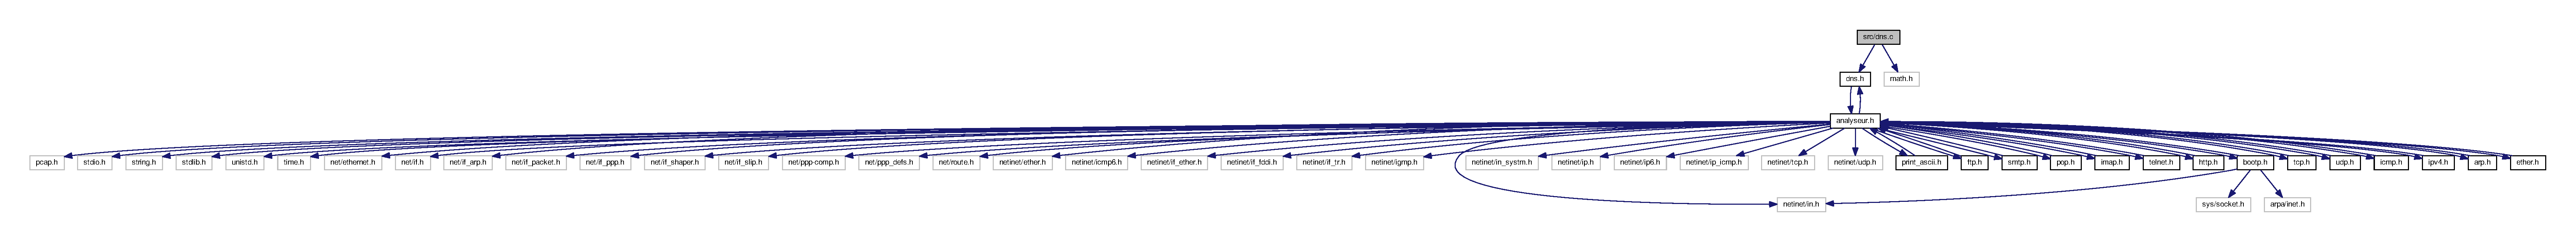
\includegraphics[width=350pt]{dns_8c__incl}
\end{center}
\end{figure}
\subsection*{Functions}
\begin{DoxyCompactItemize}
\item 
void \hyperlink{dns_8c_a936f4cda7656f30ee86c695e43582984}{affichage\+\_\+dns} (\hyperlink{struct_user}{User} $\ast$user, \hyperlink{struct_dns_hdr}{Dns\+Hdr} $\ast$hdr, const u\+\_\+char $\ast$bytes)
\item 
void \hyperlink{dns_8c_abd6805f08ec459a4a9c25ef7d718ef37}{analyse\+\_\+dns} (\hyperlink{struct_user}{User} $\ast$user, const u\+\_\+char $\ast$bytes)
\end{DoxyCompactItemize}


\subsection{Function Documentation}
\index{dns.\+c@{dns.\+c}!affichage\+\_\+dns@{affichage\+\_\+dns}}
\index{affichage\+\_\+dns@{affichage\+\_\+dns}!dns.\+c@{dns.\+c}}
\subsubsection[{\texorpdfstring{affichage\+\_\+dns(\+User $\ast$user, Dns\+Hdr $\ast$hdr, const u\+\_\+char $\ast$bytes)}{affichage_dns(User *user, DnsHdr *hdr, const u_char *bytes)}}]{\setlength{\rightskip}{0pt plus 5cm}void affichage\+\_\+dns (
\begin{DoxyParamCaption}
\item[{{\bf User} $\ast$}]{user, }
\item[{{\bf Dns\+Hdr} $\ast$}]{hdr, }
\item[{const u\+\_\+char $\ast$}]{bytes}
\end{DoxyParamCaption}
)}\hypertarget{dns_8c_a936f4cda7656f30ee86c695e43582984}{}\label{dns_8c_a936f4cda7656f30ee86c695e43582984}
\index{dns.\+c@{dns.\+c}!analyse\+\_\+dns@{analyse\+\_\+dns}}
\index{analyse\+\_\+dns@{analyse\+\_\+dns}!dns.\+c@{dns.\+c}}
\subsubsection[{\texorpdfstring{analyse\+\_\+dns(\+User $\ast$user, const u\+\_\+char $\ast$bytes)}{analyse_dns(User *user, const u_char *bytes)}}]{\setlength{\rightskip}{0pt plus 5cm}void analyse\+\_\+dns (
\begin{DoxyParamCaption}
\item[{{\bf User} $\ast$}]{user, }
\item[{const u\+\_\+char $\ast$}]{bytes}
\end{DoxyParamCaption}
)}\hypertarget{dns_8c_abd6805f08ec459a4a9c25ef7d718ef37}{}\label{dns_8c_abd6805f08ec459a4a9c25ef7d718ef37}

\hypertarget{dns_8h}{}\section{src/dns.h File Reference}
\label{dns_8h}\index{src/dns.\+h@{src/dns.\+h}}
{\ttfamily \#include \char`\"{}analyseur.\+h\char`\"{}}\\*
Include dependency graph for dns.\+h\+:
\nopagebreak
\begin{figure}[H]
\begin{center}
\leavevmode
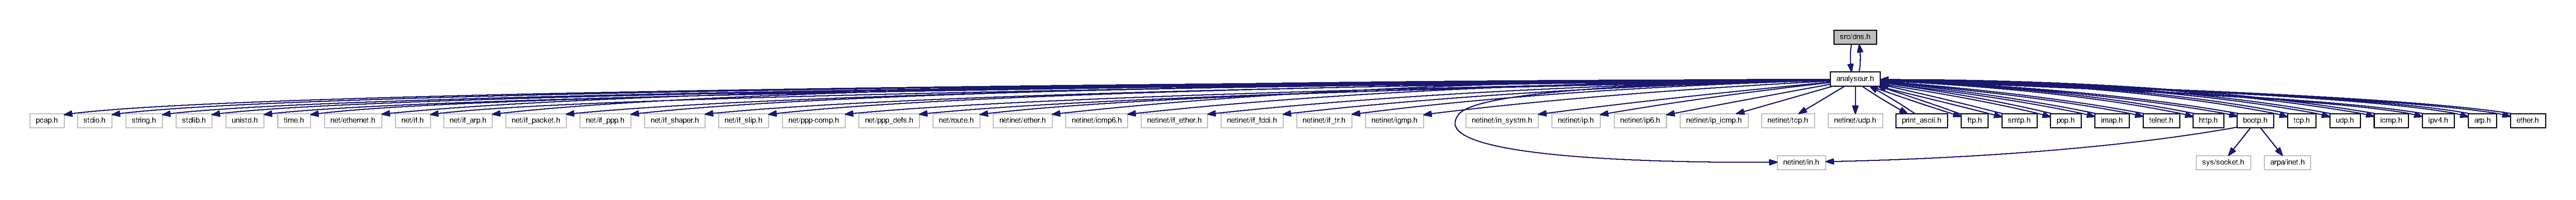
\includegraphics[width=350pt]{dns_8h__incl}
\end{center}
\end{figure}
This graph shows which files directly or indirectly include this file\+:
\nopagebreak
\begin{figure}[H]
\begin{center}
\leavevmode
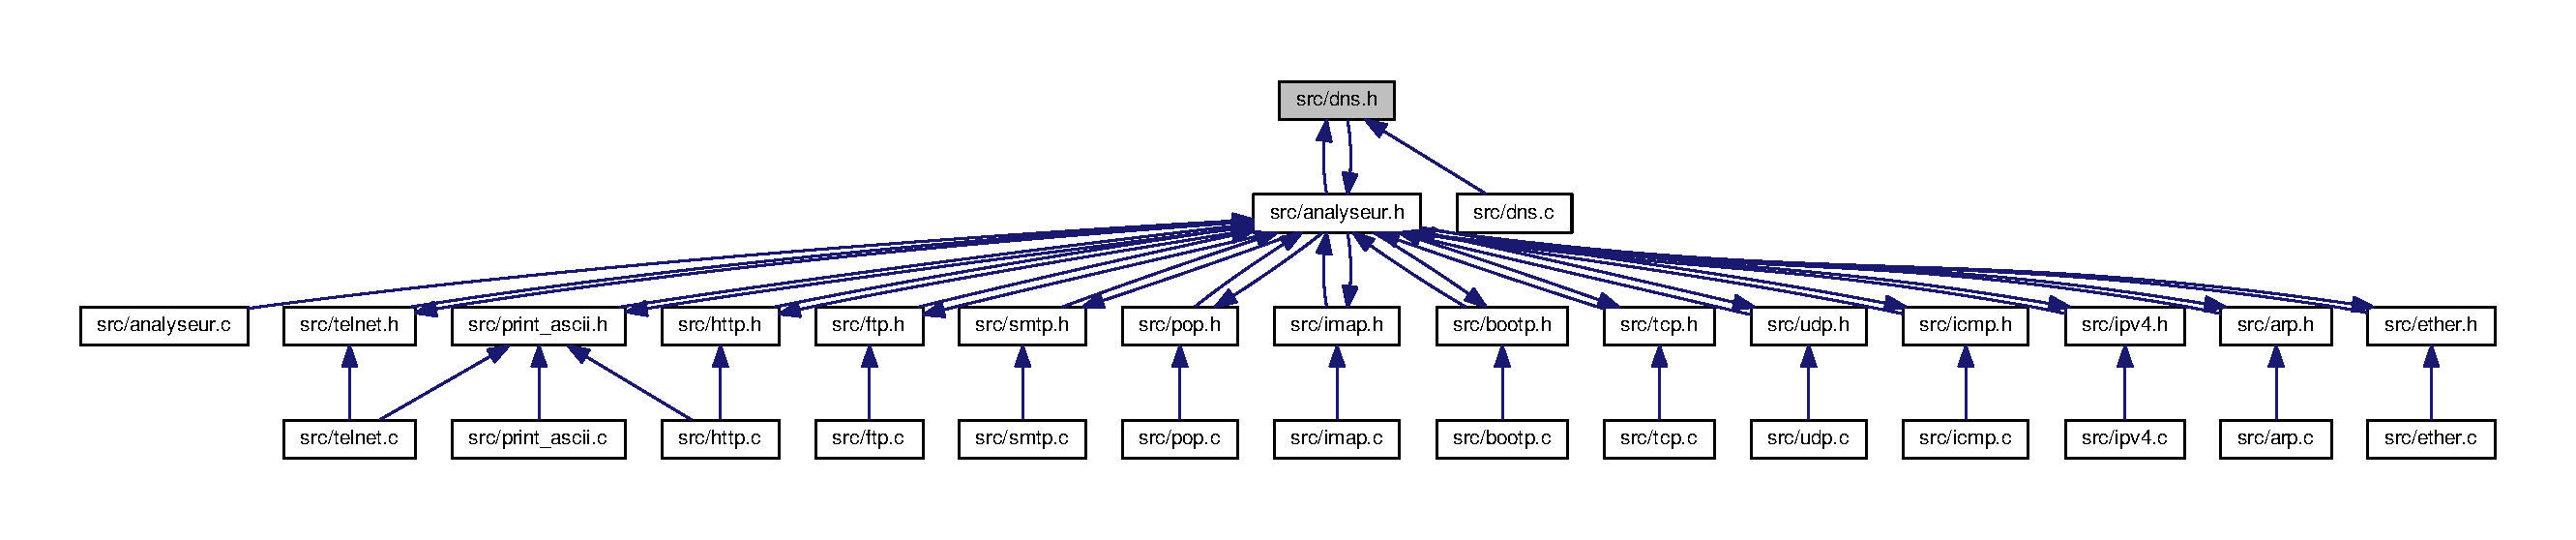
\includegraphics[width=350pt]{dns_8h__dep__incl}
\end{center}
\end{figure}
\subsection*{Data Structures}
\begin{DoxyCompactItemize}
\item 
struct \hyperlink{struct_dns_hdr}{Dns\+Hdr}
\end{DoxyCompactItemize}
\subsection*{Macros}
\begin{DoxyCompactItemize}
\item 
\#define \hyperlink{dns_8h_ac7acbb695b680e18001a814ade851327}{\+\_\+\+D\+N\+S\+\_\+}~value
\end{DoxyCompactItemize}
\subsection*{Functions}
\begin{DoxyCompactItemize}
\item 
void \hyperlink{dns_8h_abd6805f08ec459a4a9c25ef7d718ef37}{analyse\+\_\+dns} (\hyperlink{struct_user}{User} $\ast$user, const u\+\_\+char $\ast$bytes)
\end{DoxyCompactItemize}


\subsection{Macro Definition Documentation}
\index{dns.\+h@{dns.\+h}!\+\_\+\+D\+N\+S\+\_\+@{\+\_\+\+D\+N\+S\+\_\+}}
\index{\+\_\+\+D\+N\+S\+\_\+@{\+\_\+\+D\+N\+S\+\_\+}!dns.\+h@{dns.\+h}}
\subsubsection[{\texorpdfstring{\+\_\+\+D\+N\+S\+\_\+}{_DNS_}}]{\setlength{\rightskip}{0pt plus 5cm}\#define \+\_\+\+D\+N\+S\+\_\+~value}\hypertarget{dns_8h_ac7acbb695b680e18001a814ade851327}{}\label{dns_8h_ac7acbb695b680e18001a814ade851327}


\subsection{Function Documentation}
\index{dns.\+h@{dns.\+h}!analyse\+\_\+dns@{analyse\+\_\+dns}}
\index{analyse\+\_\+dns@{analyse\+\_\+dns}!dns.\+h@{dns.\+h}}
\subsubsection[{\texorpdfstring{analyse\+\_\+dns(\+User $\ast$user, const u\+\_\+char $\ast$bytes)}{analyse_dns(User *user, const u_char *bytes)}}]{\setlength{\rightskip}{0pt plus 5cm}void analyse\+\_\+dns (
\begin{DoxyParamCaption}
\item[{{\bf User} $\ast$}]{user, }
\item[{const u\+\_\+char $\ast$}]{bytes}
\end{DoxyParamCaption}
)}\hypertarget{dns_8h_abd6805f08ec459a4a9c25ef7d718ef37}{}\label{dns_8h_abd6805f08ec459a4a9c25ef7d718ef37}

\hypertarget{ether_8c}{}\section{src/ether.c File Reference}
\label{ether_8c}\index{src/ether.\+c@{src/ether.\+c}}
{\ttfamily \#include \char`\"{}ether.\+h\char`\"{}}\\*
Include dependency graph for ether.\+c\+:
\nopagebreak
\begin{figure}[H]
\begin{center}
\leavevmode
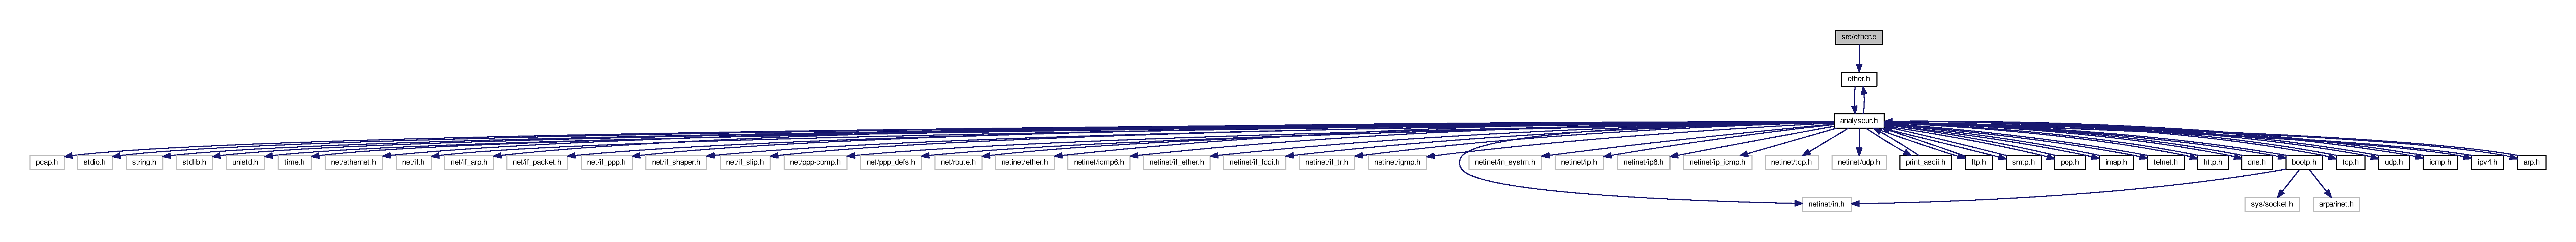
\includegraphics[width=350pt]{ether_8c__incl}
\end{center}
\end{figure}
\subsection*{Macros}
\begin{DoxyCompactItemize}
\item 
\#define \hyperlink{ether_8c_a17471f2d0d180ef15ed20835686f42bc}{E\+T\+H\+E\+R\+T\+Y\+P\+E\+\_\+\+P\+UP}~0x0200          /$\ast$ Xerox P\+U\+P $\ast$/
\end{DoxyCompactItemize}
\subsection*{Functions}
\begin{DoxyCompactItemize}
\item 
void \hyperlink{ether_8c_a4cf5ec5a6c01181557cc68ff920e0fe6}{affichage\+\_\+ethernet} (\hyperlink{struct_user}{User} $\ast$user, \hyperlink{analyseur_8h_ad90aff77137032898c538ebab55e5c76}{Ether\+Hdr} $\ast$h)
\item 
void \hyperlink{ether_8c_afb462181351d3759fbcabee6a979e940}{analyse\+\_\+ethernet} (\hyperlink{struct_user}{User} $\ast$user, const u\+\_\+char $\ast$bytes)
\end{DoxyCompactItemize}


\subsection{Macro Definition Documentation}
\index{ether.\+c@{ether.\+c}!E\+T\+H\+E\+R\+T\+Y\+P\+E\+\_\+\+P\+UP@{E\+T\+H\+E\+R\+T\+Y\+P\+E\+\_\+\+P\+UP}}
\index{E\+T\+H\+E\+R\+T\+Y\+P\+E\+\_\+\+P\+UP@{E\+T\+H\+E\+R\+T\+Y\+P\+E\+\_\+\+P\+UP}!ether.\+c@{ether.\+c}}
\subsubsection[{\texorpdfstring{E\+T\+H\+E\+R\+T\+Y\+P\+E\+\_\+\+P\+UP}{ETHERTYPE_PUP}}]{\setlength{\rightskip}{0pt plus 5cm}\#define E\+T\+H\+E\+R\+T\+Y\+P\+E\+\_\+\+P\+UP~0x0200          /$\ast$ Xerox P\+U\+P $\ast$/}\hypertarget{ether_8c_a17471f2d0d180ef15ed20835686f42bc}{}\label{ether_8c_a17471f2d0d180ef15ed20835686f42bc}


\subsection{Function Documentation}
\index{ether.\+c@{ether.\+c}!affichage\+\_\+ethernet@{affichage\+\_\+ethernet}}
\index{affichage\+\_\+ethernet@{affichage\+\_\+ethernet}!ether.\+c@{ether.\+c}}
\subsubsection[{\texorpdfstring{affichage\+\_\+ethernet(\+User $\ast$user, Ether\+Hdr $\ast$h)}{affichage_ethernet(User *user, EtherHdr *h)}}]{\setlength{\rightskip}{0pt plus 5cm}void affichage\+\_\+ethernet (
\begin{DoxyParamCaption}
\item[{{\bf User} $\ast$}]{user, }
\item[{{\bf Ether\+Hdr} $\ast$}]{h}
\end{DoxyParamCaption}
)}\hypertarget{ether_8c_a4cf5ec5a6c01181557cc68ff920e0fe6}{}\label{ether_8c_a4cf5ec5a6c01181557cc68ff920e0fe6}
\index{ether.\+c@{ether.\+c}!analyse\+\_\+ethernet@{analyse\+\_\+ethernet}}
\index{analyse\+\_\+ethernet@{analyse\+\_\+ethernet}!ether.\+c@{ether.\+c}}
\subsubsection[{\texorpdfstring{analyse\+\_\+ethernet(\+User $\ast$user, const u\+\_\+char $\ast$bytes)}{analyse_ethernet(User *user, const u_char *bytes)}}]{\setlength{\rightskip}{0pt plus 5cm}void analyse\+\_\+ethernet (
\begin{DoxyParamCaption}
\item[{{\bf User} $\ast$}]{user, }
\item[{const u\+\_\+char $\ast$}]{bytes}
\end{DoxyParamCaption}
)}\hypertarget{ether_8c_afb462181351d3759fbcabee6a979e940}{}\label{ether_8c_afb462181351d3759fbcabee6a979e940}

\hypertarget{ether_8h}{}\section{src/ether.h File Reference}
\label{ether_8h}\index{src/ether.\+h@{src/ether.\+h}}
{\ttfamily \#include \char`\"{}analyseur.\+h\char`\"{}}\\*
Include dependency graph for ether.\+h\+:
\nopagebreak
\begin{figure}[H]
\begin{center}
\leavevmode
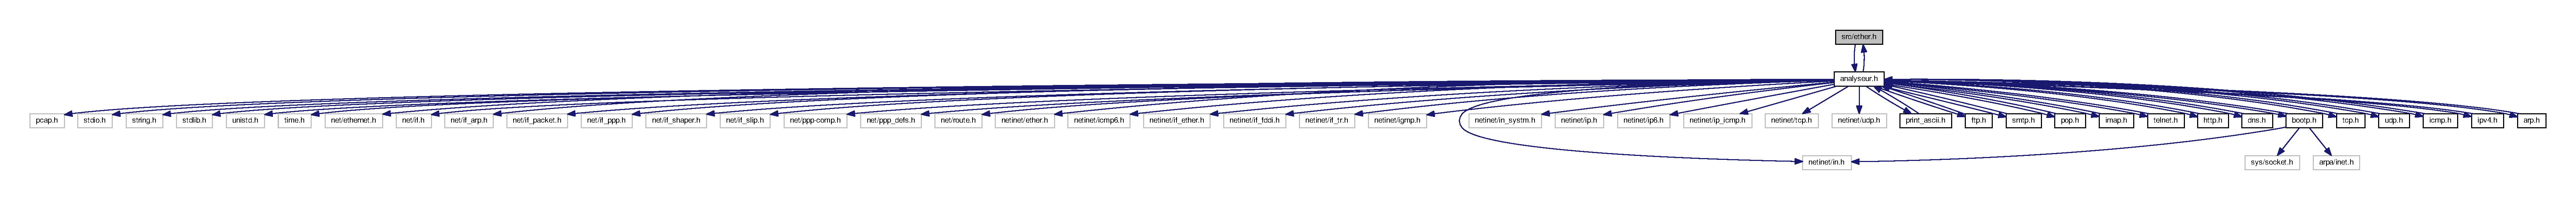
\includegraphics[width=350pt]{ether_8h__incl}
\end{center}
\end{figure}
This graph shows which files directly or indirectly include this file\+:
\nopagebreak
\begin{figure}[H]
\begin{center}
\leavevmode
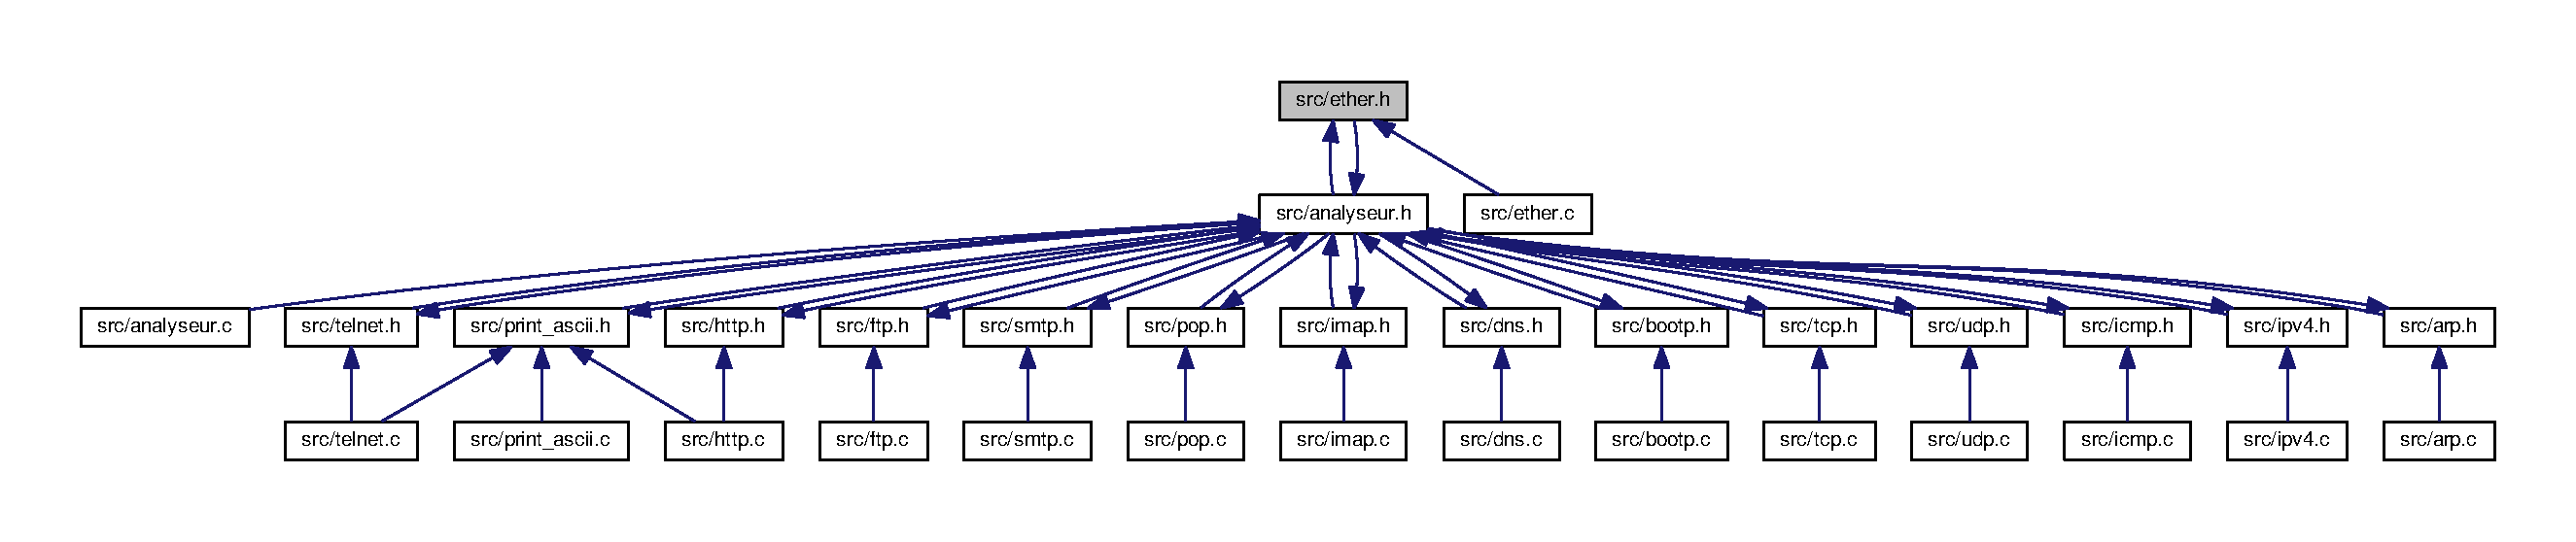
\includegraphics[width=350pt]{ether_8h__dep__incl}
\end{center}
\end{figure}
\subsection*{Functions}
\begin{DoxyCompactItemize}
\item 
void \hyperlink{ether_8h_afb462181351d3759fbcabee6a979e940}{analyse\+\_\+ethernet} (\hyperlink{struct_user}{User} $\ast$user, const u\+\_\+char $\ast$bytes)
\end{DoxyCompactItemize}


\subsection{Function Documentation}
\index{ether.\+h@{ether.\+h}!analyse\+\_\+ethernet@{analyse\+\_\+ethernet}}
\index{analyse\+\_\+ethernet@{analyse\+\_\+ethernet}!ether.\+h@{ether.\+h}}
\subsubsection[{\texorpdfstring{analyse\+\_\+ethernet(\+User $\ast$user, const u\+\_\+char $\ast$bytes)}{analyse_ethernet(User *user, const u_char *bytes)}}]{\setlength{\rightskip}{0pt plus 5cm}void analyse\+\_\+ethernet (
\begin{DoxyParamCaption}
\item[{{\bf User} $\ast$}]{user, }
\item[{const u\+\_\+char $\ast$}]{bytes}
\end{DoxyParamCaption}
)}\hypertarget{ether_8h_afb462181351d3759fbcabee6a979e940}{}\label{ether_8h_afb462181351d3759fbcabee6a979e940}

\hypertarget{ftp_8c}{}\section{src/ftp.c File Reference}
\label{ftp_8c}\index{src/ftp.\+c@{src/ftp.\+c}}
{\ttfamily \#include \char`\"{}ftp.\+h\char`\"{}}\\*
Include dependency graph for ftp.\+c\+:
\nopagebreak
\begin{figure}[H]
\begin{center}
\leavevmode
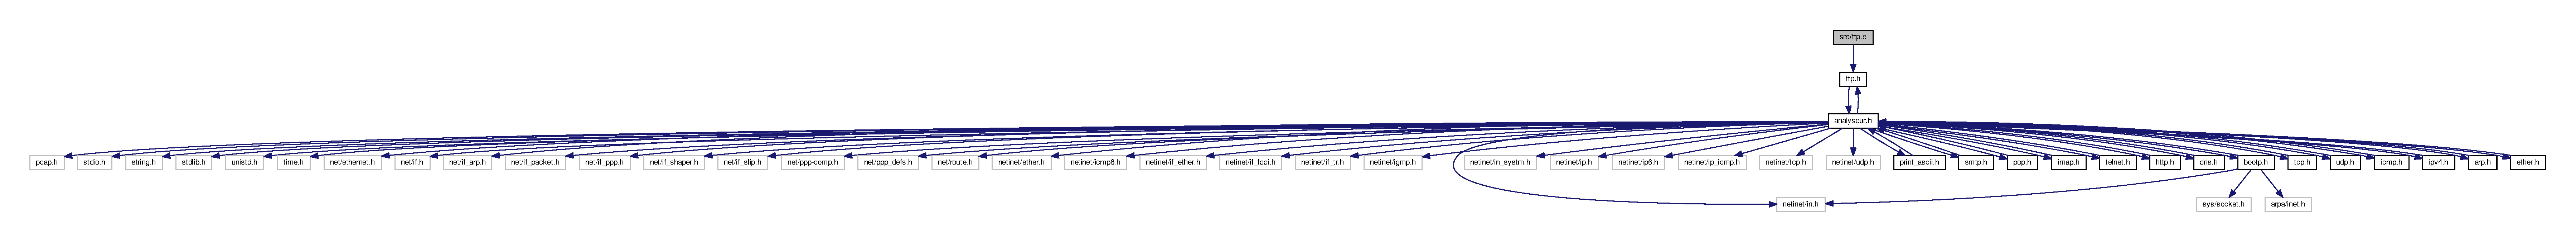
\includegraphics[width=350pt]{ftp_8c__incl}
\end{center}
\end{figure}
\subsection*{Functions}
\begin{DoxyCompactItemize}
\item 
void \hyperlink{ftp_8c_a887dc86a52d29692a35e086e9817d6f5}{affichage\+\_\+ftp} (\hyperlink{struct_user}{User} $\ast$user, const u\+\_\+char $\ast$bytes)
\item 
void \hyperlink{ftp_8c_ade8a5111360f542e082f07ed46084093}{analyse\+\_\+ftp} (\hyperlink{struct_user}{User} $\ast$user, const u\+\_\+char $\ast$bytes)
\end{DoxyCompactItemize}


\subsection{Function Documentation}
\index{ftp.\+c@{ftp.\+c}!affichage\+\_\+ftp@{affichage\+\_\+ftp}}
\index{affichage\+\_\+ftp@{affichage\+\_\+ftp}!ftp.\+c@{ftp.\+c}}
\subsubsection[{\texorpdfstring{affichage\+\_\+ftp(\+User $\ast$user, const u\+\_\+char $\ast$bytes)}{affichage_ftp(User *user, const u_char *bytes)}}]{\setlength{\rightskip}{0pt plus 5cm}void affichage\+\_\+ftp (
\begin{DoxyParamCaption}
\item[{{\bf User} $\ast$}]{user, }
\item[{const u\+\_\+char $\ast$}]{bytes}
\end{DoxyParamCaption}
)}\hypertarget{ftp_8c_a887dc86a52d29692a35e086e9817d6f5}{}\label{ftp_8c_a887dc86a52d29692a35e086e9817d6f5}
\index{ftp.\+c@{ftp.\+c}!analyse\+\_\+ftp@{analyse\+\_\+ftp}}
\index{analyse\+\_\+ftp@{analyse\+\_\+ftp}!ftp.\+c@{ftp.\+c}}
\subsubsection[{\texorpdfstring{analyse\+\_\+ftp(\+User $\ast$user, const u\+\_\+char $\ast$bytes)}{analyse_ftp(User *user, const u_char *bytes)}}]{\setlength{\rightskip}{0pt plus 5cm}void analyse\+\_\+ftp (
\begin{DoxyParamCaption}
\item[{{\bf User} $\ast$}]{user, }
\item[{const u\+\_\+char $\ast$}]{bytes}
\end{DoxyParamCaption}
)}\hypertarget{ftp_8c_ade8a5111360f542e082f07ed46084093}{}\label{ftp_8c_ade8a5111360f542e082f07ed46084093}

\hypertarget{ftp_8h}{}\section{src/ftp.h File Reference}
\label{ftp_8h}\index{src/ftp.\+h@{src/ftp.\+h}}
{\ttfamily \#include \char`\"{}analyseur.\+h\char`\"{}}\\*
Include dependency graph for ftp.\+h\+:
\nopagebreak
\begin{figure}[H]
\begin{center}
\leavevmode
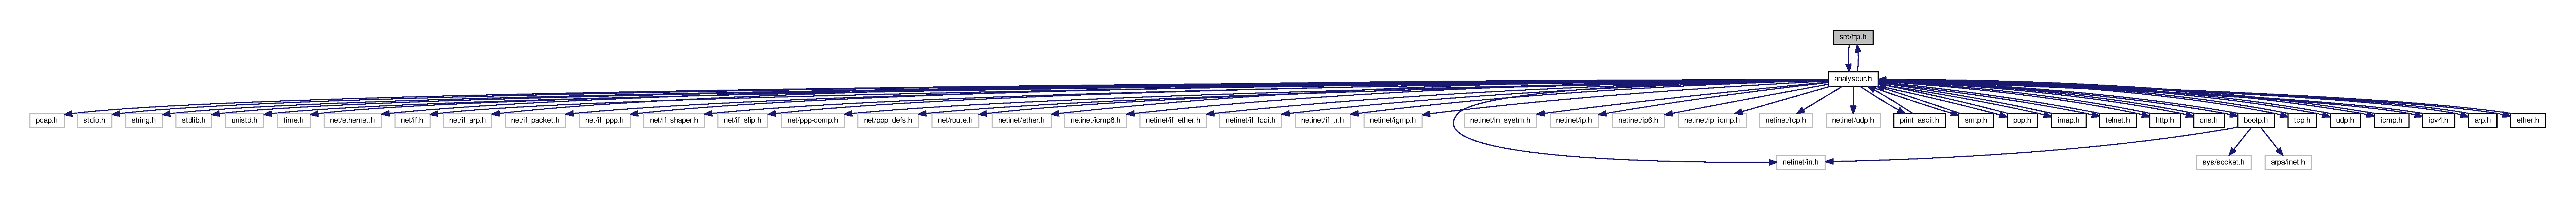
\includegraphics[width=350pt]{ftp_8h__incl}
\end{center}
\end{figure}
This graph shows which files directly or indirectly include this file\+:
\nopagebreak
\begin{figure}[H]
\begin{center}
\leavevmode
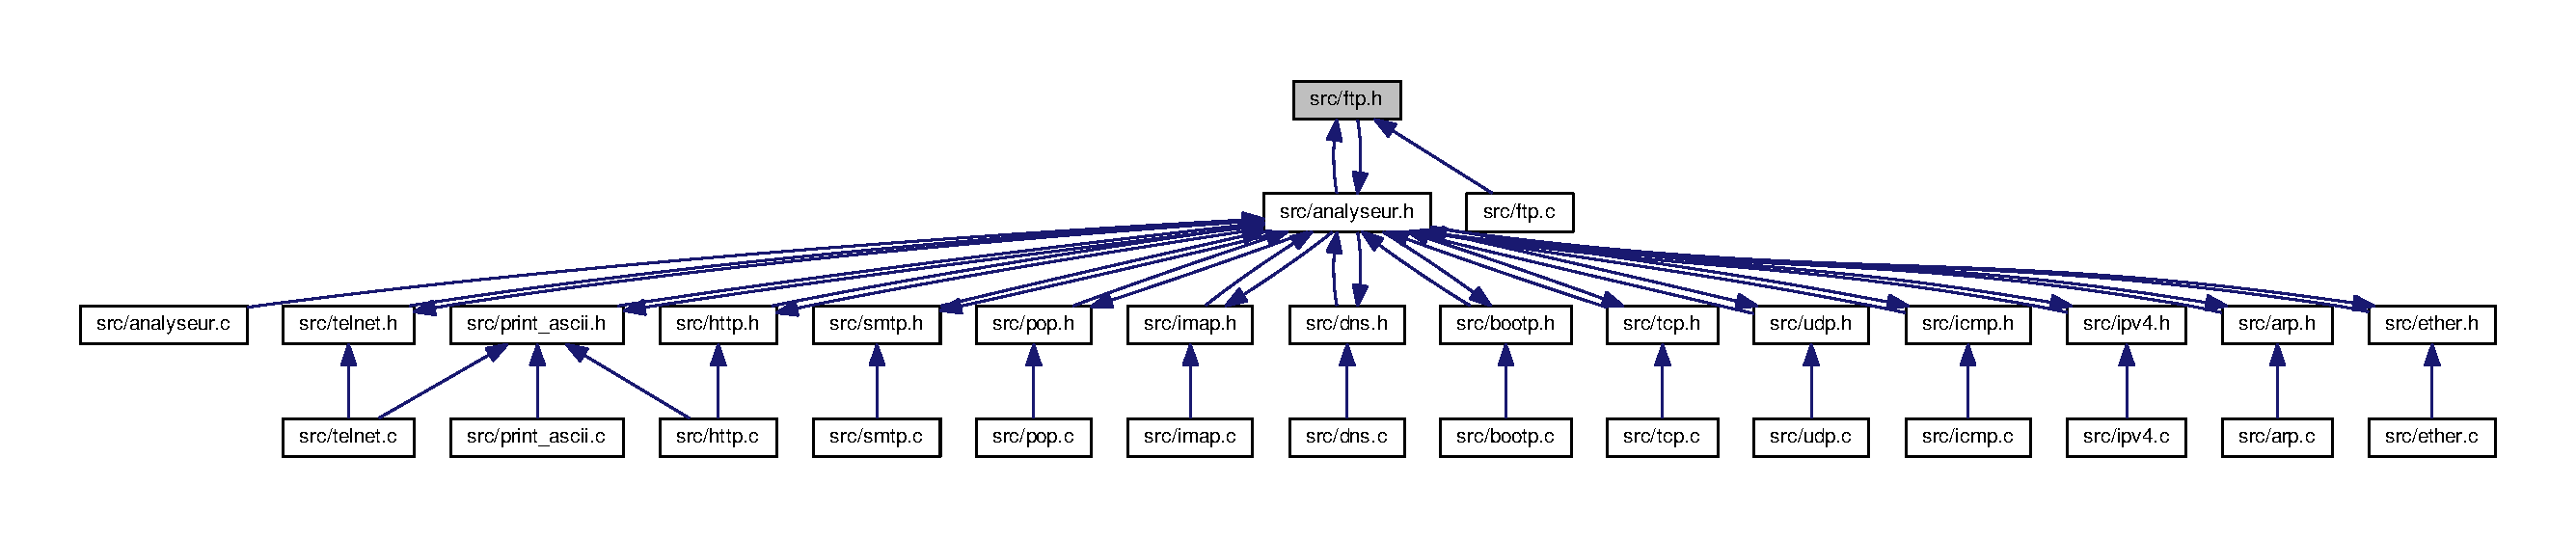
\includegraphics[width=350pt]{ftp_8h__dep__incl}
\end{center}
\end{figure}
\subsection*{Functions}
\begin{DoxyCompactItemize}
\item 
void \hyperlink{ftp_8h_ade8a5111360f542e082f07ed46084093}{analyse\+\_\+ftp} (\hyperlink{struct_user}{User} $\ast$user, const u\+\_\+char $\ast$bytes)
\end{DoxyCompactItemize}


\subsection{Function Documentation}
\index{ftp.\+h@{ftp.\+h}!analyse\+\_\+ftp@{analyse\+\_\+ftp}}
\index{analyse\+\_\+ftp@{analyse\+\_\+ftp}!ftp.\+h@{ftp.\+h}}
\subsubsection[{\texorpdfstring{analyse\+\_\+ftp(\+User $\ast$user, const u\+\_\+char $\ast$bytes)}{analyse_ftp(User *user, const u_char *bytes)}}]{\setlength{\rightskip}{0pt plus 5cm}void analyse\+\_\+ftp (
\begin{DoxyParamCaption}
\item[{{\bf User} $\ast$}]{user, }
\item[{const u\+\_\+char $\ast$}]{bytes}
\end{DoxyParamCaption}
)}\hypertarget{ftp_8h_ade8a5111360f542e082f07ed46084093}{}\label{ftp_8h_ade8a5111360f542e082f07ed46084093}

\hypertarget{http_8c}{}\section{src/http.c File Reference}
\label{http_8c}\index{src/http.\+c@{src/http.\+c}}
{\ttfamily \#include \char`\"{}http.\+h\char`\"{}}\\*
{\ttfamily \#include \char`\"{}print\+\_\+ascii.\+h\char`\"{}}\\*
{\ttfamily \#include $<$ctype.\+h$>$}\\*
Include dependency graph for http.\+c\+:
\nopagebreak
\begin{figure}[H]
\begin{center}
\leavevmode
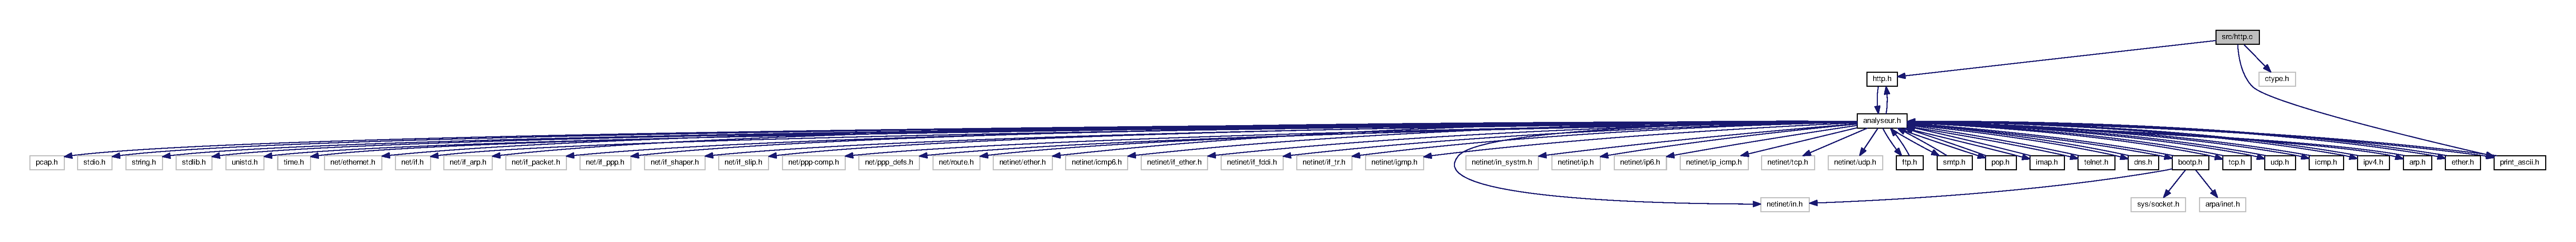
\includegraphics[width=350pt]{http_8c__incl}
\end{center}
\end{figure}
\subsection*{Functions}
\begin{DoxyCompactItemize}
\item 
void \hyperlink{http_8c_a5a4671827d51b90e98c600a4fe2494c2}{affichage\+\_\+http} (\hyperlink{struct_user}{User} $\ast$user, const u\+\_\+char $\ast$bytes)
\item 
void \hyperlink{http_8c_aeb962a45d57fc1853fbf47113f59e582}{analyse\+\_\+http} (\hyperlink{struct_user}{User} $\ast$user, const u\+\_\+char $\ast$bytes)
\end{DoxyCompactItemize}


\subsection{Function Documentation}
\index{http.\+c@{http.\+c}!affichage\+\_\+http@{affichage\+\_\+http}}
\index{affichage\+\_\+http@{affichage\+\_\+http}!http.\+c@{http.\+c}}
\subsubsection[{\texorpdfstring{affichage\+\_\+http(\+User $\ast$user, const u\+\_\+char $\ast$bytes)}{affichage_http(User *user, const u_char *bytes)}}]{\setlength{\rightskip}{0pt plus 5cm}void affichage\+\_\+http (
\begin{DoxyParamCaption}
\item[{{\bf User} $\ast$}]{user, }
\item[{const u\+\_\+char $\ast$}]{bytes}
\end{DoxyParamCaption}
)}\hypertarget{http_8c_a5a4671827d51b90e98c600a4fe2494c2}{}\label{http_8c_a5a4671827d51b90e98c600a4fe2494c2}
\index{http.\+c@{http.\+c}!analyse\+\_\+http@{analyse\+\_\+http}}
\index{analyse\+\_\+http@{analyse\+\_\+http}!http.\+c@{http.\+c}}
\subsubsection[{\texorpdfstring{analyse\+\_\+http(\+User $\ast$user, const u\+\_\+char $\ast$bytes)}{analyse_http(User *user, const u_char *bytes)}}]{\setlength{\rightskip}{0pt plus 5cm}void analyse\+\_\+http (
\begin{DoxyParamCaption}
\item[{{\bf User} $\ast$}]{user, }
\item[{const u\+\_\+char $\ast$}]{bytes}
\end{DoxyParamCaption}
)}\hypertarget{http_8c_aeb962a45d57fc1853fbf47113f59e582}{}\label{http_8c_aeb962a45d57fc1853fbf47113f59e582}

\hypertarget{http_8h}{}\section{src/http.h File Reference}
\label{http_8h}\index{src/http.\+h@{src/http.\+h}}
{\ttfamily \#include \char`\"{}analyseur.\+h\char`\"{}}\\*
Include dependency graph for http.\+h\+:
\nopagebreak
\begin{figure}[H]
\begin{center}
\leavevmode
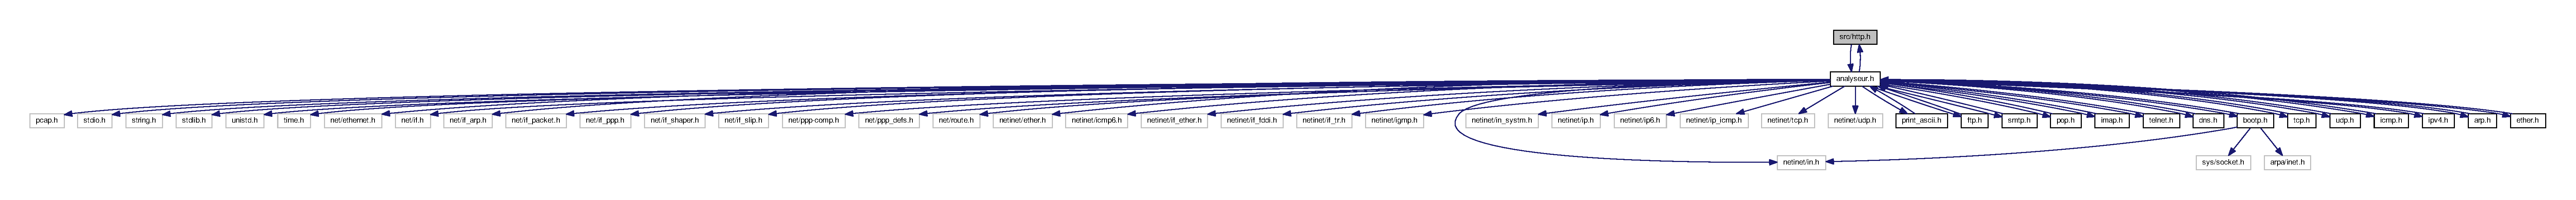
\includegraphics[width=350pt]{http_8h__incl}
\end{center}
\end{figure}
This graph shows which files directly or indirectly include this file\+:
\nopagebreak
\begin{figure}[H]
\begin{center}
\leavevmode
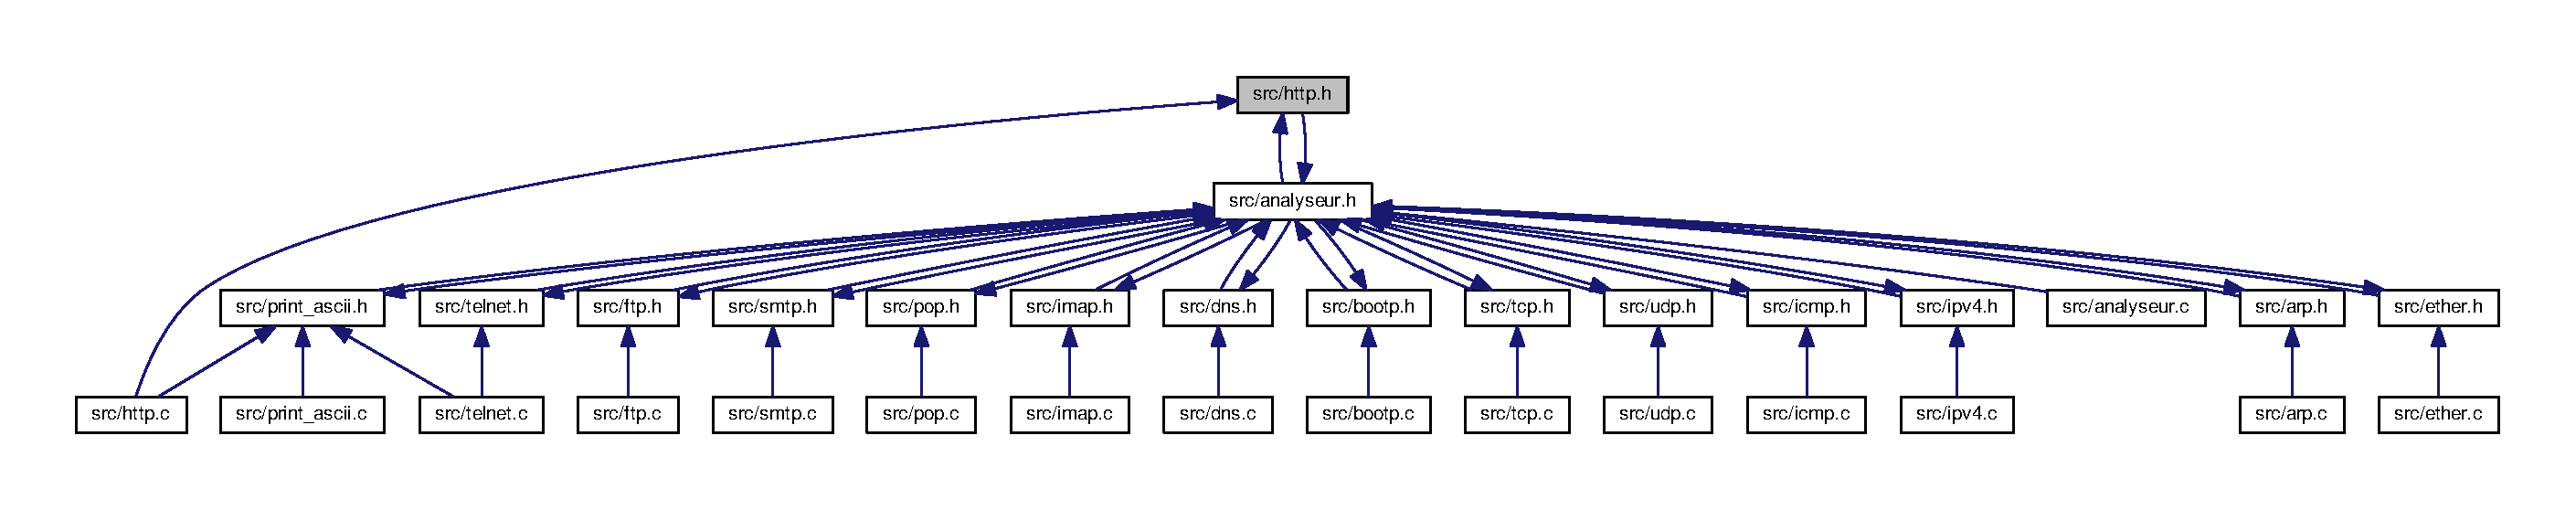
\includegraphics[width=350pt]{http_8h__dep__incl}
\end{center}
\end{figure}
\subsection*{Functions}
\begin{DoxyCompactItemize}
\item 
void \hyperlink{http_8h_aeb962a45d57fc1853fbf47113f59e582}{analyse\+\_\+http} (\hyperlink{struct_user}{User} $\ast$user, const u\+\_\+char $\ast$bytes)
\end{DoxyCompactItemize}


\subsection{Function Documentation}
\index{http.\+h@{http.\+h}!analyse\+\_\+http@{analyse\+\_\+http}}
\index{analyse\+\_\+http@{analyse\+\_\+http}!http.\+h@{http.\+h}}
\subsubsection[{\texorpdfstring{analyse\+\_\+http(\+User $\ast$user, const u\+\_\+char $\ast$bytes)}{analyse_http(User *user, const u_char *bytes)}}]{\setlength{\rightskip}{0pt plus 5cm}void analyse\+\_\+http (
\begin{DoxyParamCaption}
\item[{{\bf User} $\ast$}]{user, }
\item[{const u\+\_\+char $\ast$}]{bytes}
\end{DoxyParamCaption}
)}\hypertarget{http_8h_aeb962a45d57fc1853fbf47113f59e582}{}\label{http_8h_aeb962a45d57fc1853fbf47113f59e582}

\hypertarget{icmp_8c}{}\section{src/icmp.c File Reference}
\label{icmp_8c}\index{src/icmp.\+c@{src/icmp.\+c}}
{\ttfamily \#include \char`\"{}icmp.\+h\char`\"{}}\\*
Include dependency graph for icmp.\+c\+:
\nopagebreak
\begin{figure}[H]
\begin{center}
\leavevmode
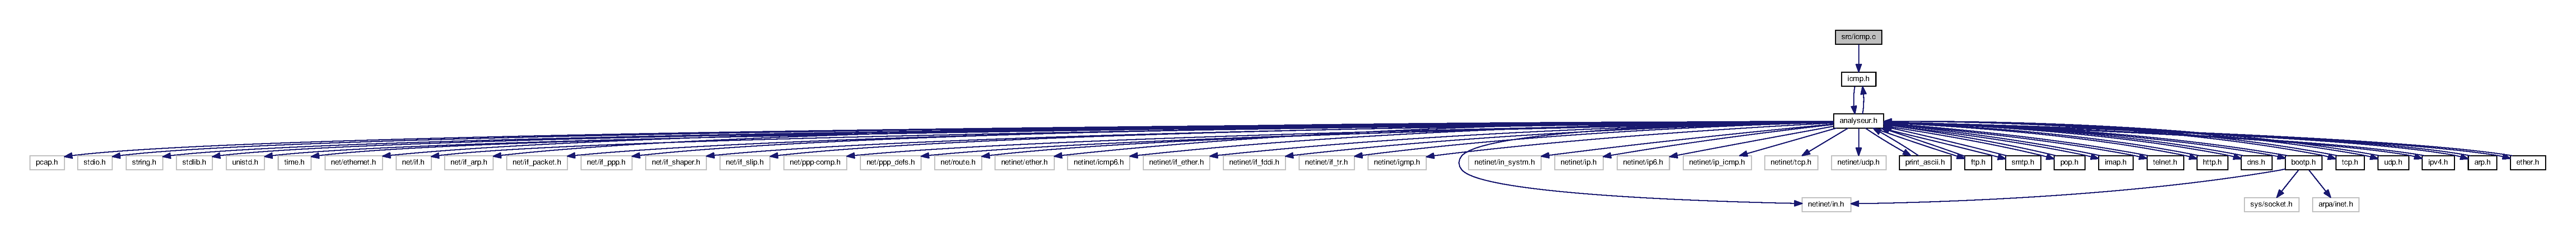
\includegraphics[width=350pt]{icmp_8c__incl}
\end{center}
\end{figure}
\subsection*{Functions}
\begin{DoxyCompactItemize}
\item 
void \hyperlink{icmp_8c_af86c14200551be2597cb37e36ee5a4f0}{affichage\+\_\+icmp} (\hyperlink{struct_user}{User} $\ast$user, \hyperlink{analyseur_8h_ac69a3725cff99f912ce0d4281b5b4ea7}{Icmp\+Hdr} $\ast$icmphdr)
\item 
void \hyperlink{icmp_8c_a64243289dc7fbfa90c91a73296e9d715}{analyse\+\_\+icmp} (\hyperlink{struct_user}{User} $\ast$user, const u\+\_\+char $\ast$bytes)
\end{DoxyCompactItemize}


\subsection{Function Documentation}
\index{icmp.\+c@{icmp.\+c}!affichage\+\_\+icmp@{affichage\+\_\+icmp}}
\index{affichage\+\_\+icmp@{affichage\+\_\+icmp}!icmp.\+c@{icmp.\+c}}
\subsubsection[{\texorpdfstring{affichage\+\_\+icmp(\+User $\ast$user, Icmp\+Hdr $\ast$icmphdr)}{affichage_icmp(User *user, IcmpHdr *icmphdr)}}]{\setlength{\rightskip}{0pt plus 5cm}void affichage\+\_\+icmp (
\begin{DoxyParamCaption}
\item[{{\bf User} $\ast$}]{user, }
\item[{{\bf Icmp\+Hdr} $\ast$}]{icmphdr}
\end{DoxyParamCaption}
)}\hypertarget{icmp_8c_af86c14200551be2597cb37e36ee5a4f0}{}\label{icmp_8c_af86c14200551be2597cb37e36ee5a4f0}
\index{icmp.\+c@{icmp.\+c}!analyse\+\_\+icmp@{analyse\+\_\+icmp}}
\index{analyse\+\_\+icmp@{analyse\+\_\+icmp}!icmp.\+c@{icmp.\+c}}
\subsubsection[{\texorpdfstring{analyse\+\_\+icmp(\+User $\ast$user, const u\+\_\+char $\ast$bytes)}{analyse_icmp(User *user, const u_char *bytes)}}]{\setlength{\rightskip}{0pt plus 5cm}void analyse\+\_\+icmp (
\begin{DoxyParamCaption}
\item[{{\bf User} $\ast$}]{user, }
\item[{const u\+\_\+char $\ast$}]{bytes}
\end{DoxyParamCaption}
)}\hypertarget{icmp_8c_a64243289dc7fbfa90c91a73296e9d715}{}\label{icmp_8c_a64243289dc7fbfa90c91a73296e9d715}

\hypertarget{icmp_8h}{}\section{src/icmp.h File Reference}
\label{icmp_8h}\index{src/icmp.\+h@{src/icmp.\+h}}
{\ttfamily \#include \char`\"{}analyseur.\+h\char`\"{}}\\*
Include dependency graph for icmp.\+h\+:
\nopagebreak
\begin{figure}[H]
\begin{center}
\leavevmode
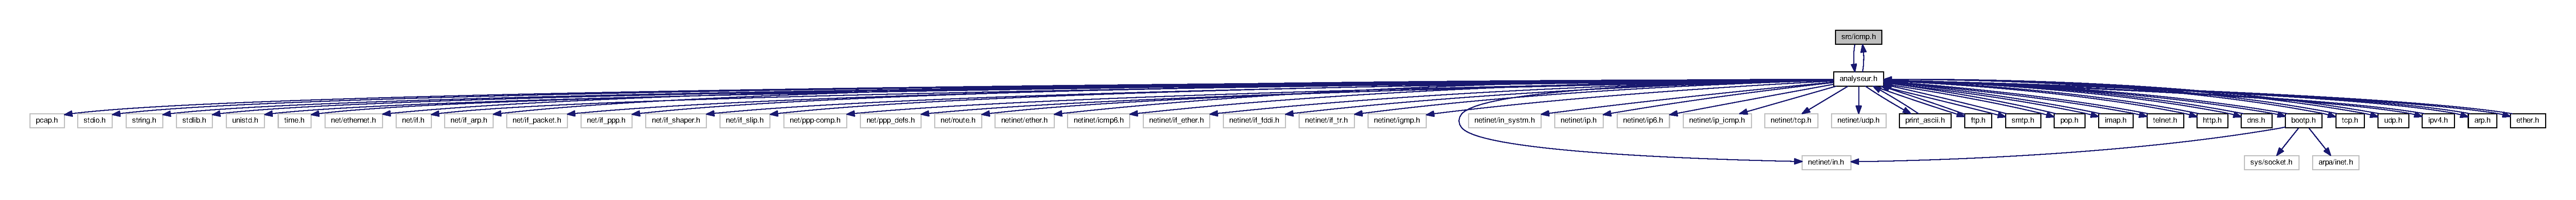
\includegraphics[width=350pt]{icmp_8h__incl}
\end{center}
\end{figure}
This graph shows which files directly or indirectly include this file\+:
\nopagebreak
\begin{figure}[H]
\begin{center}
\leavevmode
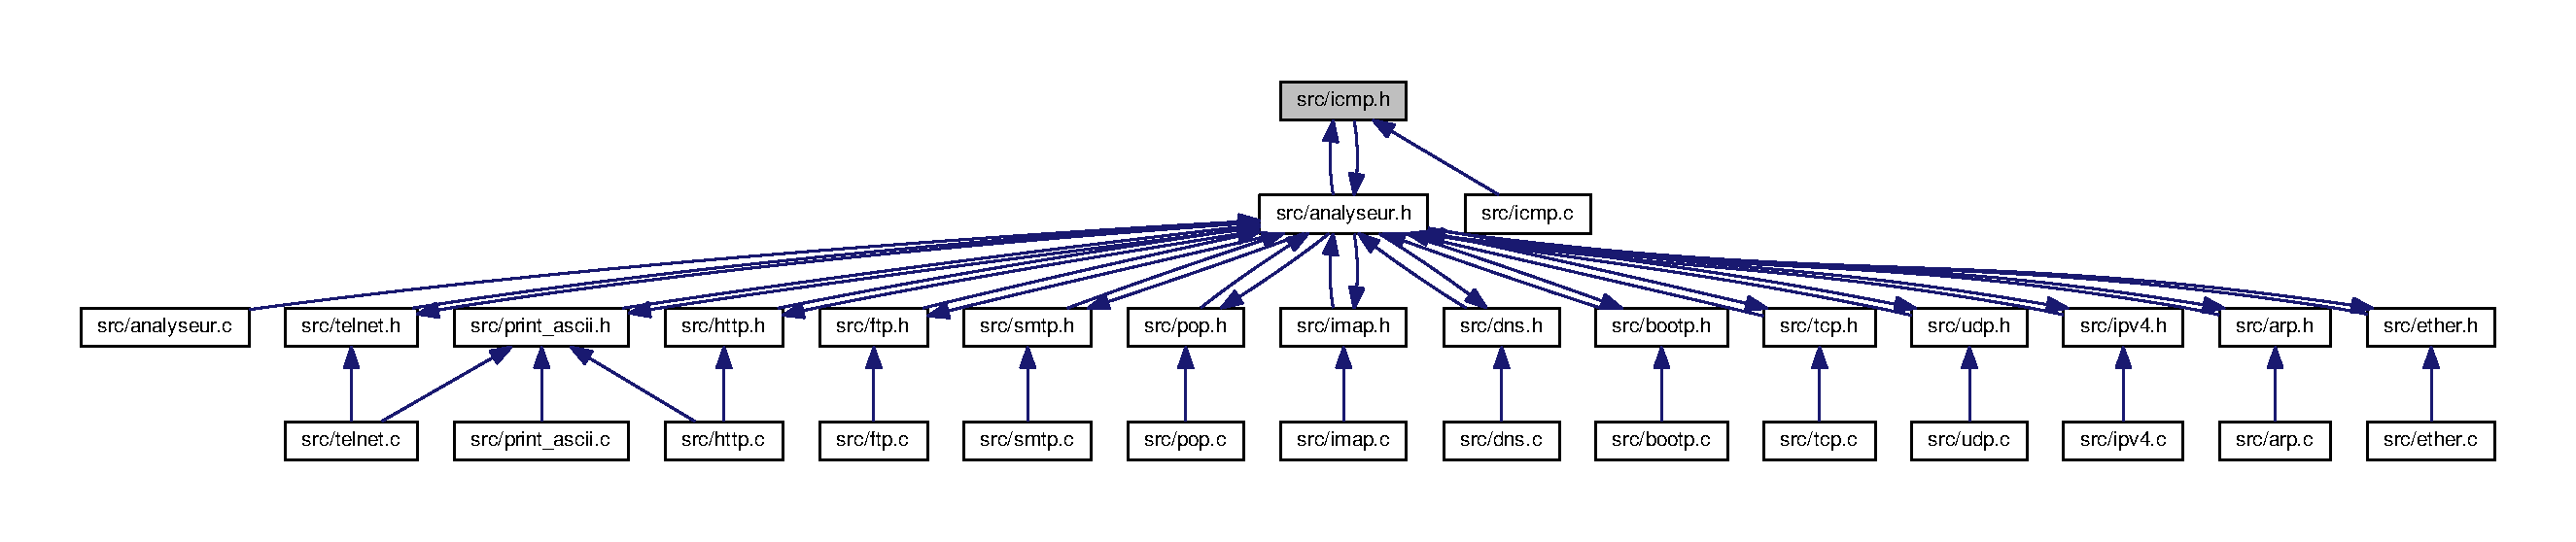
\includegraphics[width=350pt]{icmp_8h__dep__incl}
\end{center}
\end{figure}
\subsection*{Functions}
\begin{DoxyCompactItemize}
\item 
void \hyperlink{icmp_8h_a64243289dc7fbfa90c91a73296e9d715}{analyse\+\_\+icmp} (\hyperlink{struct_user}{User} $\ast$user, const u\+\_\+char $\ast$bytes)
\end{DoxyCompactItemize}


\subsection{Function Documentation}
\index{icmp.\+h@{icmp.\+h}!analyse\+\_\+icmp@{analyse\+\_\+icmp}}
\index{analyse\+\_\+icmp@{analyse\+\_\+icmp}!icmp.\+h@{icmp.\+h}}
\subsubsection[{\texorpdfstring{analyse\+\_\+icmp(\+User $\ast$user, const u\+\_\+char $\ast$bytes)}{analyse_icmp(User *user, const u_char *bytes)}}]{\setlength{\rightskip}{0pt plus 5cm}void analyse\+\_\+icmp (
\begin{DoxyParamCaption}
\item[{{\bf User} $\ast$}]{user, }
\item[{const u\+\_\+char $\ast$}]{bytes}
\end{DoxyParamCaption}
)}\hypertarget{icmp_8h_a64243289dc7fbfa90c91a73296e9d715}{}\label{icmp_8h_a64243289dc7fbfa90c91a73296e9d715}

\hypertarget{imap_8c}{}\section{src/imap.c File Reference}
\label{imap_8c}\index{src/imap.\+c@{src/imap.\+c}}
{\ttfamily \#include \char`\"{}imap.\+h\char`\"{}}\\*
Include dependency graph for imap.\+c\+:
\nopagebreak
\begin{figure}[H]
\begin{center}
\leavevmode
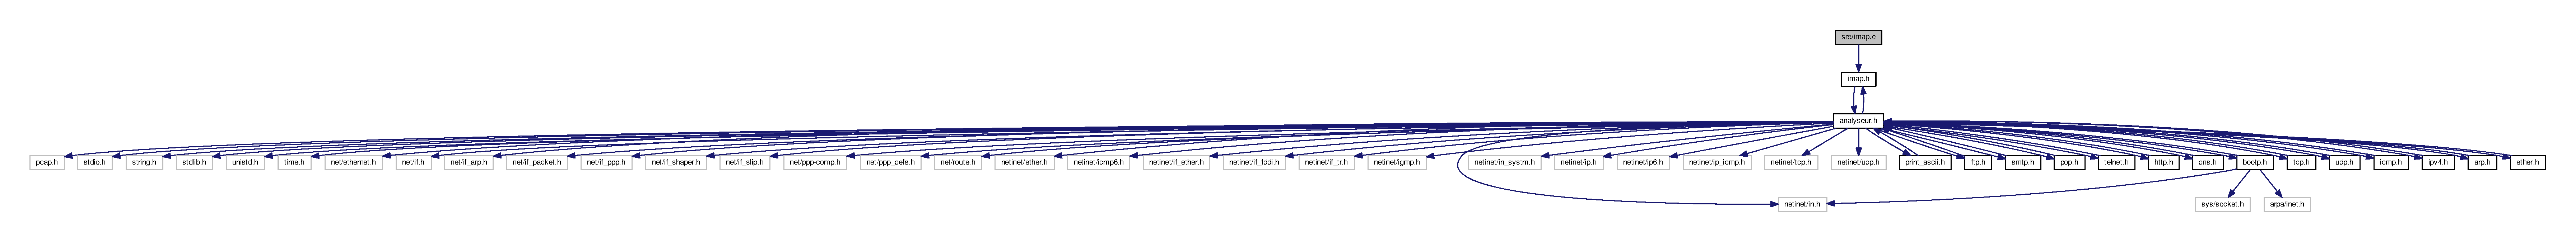
\includegraphics[width=350pt]{imap_8c__incl}
\end{center}
\end{figure}
\subsection*{Functions}
\begin{DoxyCompactItemize}
\item 
void \hyperlink{imap_8c_ac505b244c310b52bdafa82c024ea9d6c}{affichage\+\_\+imap} (\hyperlink{struct_user}{User} $\ast$user, const u\+\_\+char $\ast$bytes)
\item 
void \hyperlink{imap_8c_a2f858f7da61dd47b3dc3be95f9eb2d3a}{analyse\+\_\+imap} (\hyperlink{struct_user}{User} $\ast$user, const u\+\_\+char $\ast$bytes)
\end{DoxyCompactItemize}


\subsection{Function Documentation}
\index{imap.\+c@{imap.\+c}!affichage\+\_\+imap@{affichage\+\_\+imap}}
\index{affichage\+\_\+imap@{affichage\+\_\+imap}!imap.\+c@{imap.\+c}}
\subsubsection[{\texorpdfstring{affichage\+\_\+imap(\+User $\ast$user, const u\+\_\+char $\ast$bytes)}{affichage_imap(User *user, const u_char *bytes)}}]{\setlength{\rightskip}{0pt plus 5cm}void affichage\+\_\+imap (
\begin{DoxyParamCaption}
\item[{{\bf User} $\ast$}]{user, }
\item[{const u\+\_\+char $\ast$}]{bytes}
\end{DoxyParamCaption}
)}\hypertarget{imap_8c_ac505b244c310b52bdafa82c024ea9d6c}{}\label{imap_8c_ac505b244c310b52bdafa82c024ea9d6c}
\index{imap.\+c@{imap.\+c}!analyse\+\_\+imap@{analyse\+\_\+imap}}
\index{analyse\+\_\+imap@{analyse\+\_\+imap}!imap.\+c@{imap.\+c}}
\subsubsection[{\texorpdfstring{analyse\+\_\+imap(\+User $\ast$user, const u\+\_\+char $\ast$bytes)}{analyse_imap(User *user, const u_char *bytes)}}]{\setlength{\rightskip}{0pt plus 5cm}void analyse\+\_\+imap (
\begin{DoxyParamCaption}
\item[{{\bf User} $\ast$}]{user, }
\item[{const u\+\_\+char $\ast$}]{bytes}
\end{DoxyParamCaption}
)}\hypertarget{imap_8c_a2f858f7da61dd47b3dc3be95f9eb2d3a}{}\label{imap_8c_a2f858f7da61dd47b3dc3be95f9eb2d3a}

\hypertarget{imap_8h}{}\section{src/imap.h File Reference}
\label{imap_8h}\index{src/imap.\+h@{src/imap.\+h}}
{\ttfamily \#include \char`\"{}analyseur.\+h\char`\"{}}\\*
Include dependency graph for imap.\+h\+:
\nopagebreak
\begin{figure}[H]
\begin{center}
\leavevmode
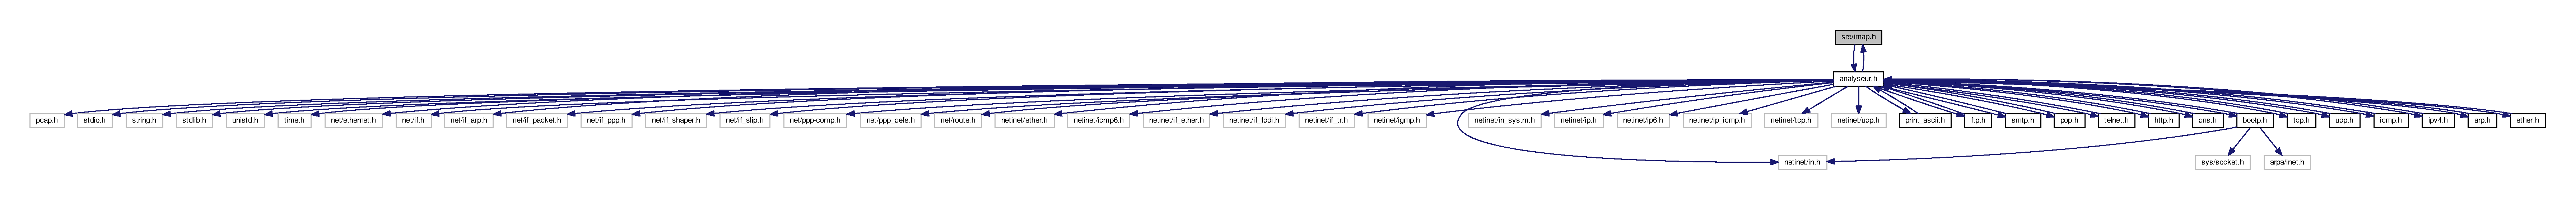
\includegraphics[width=350pt]{imap_8h__incl}
\end{center}
\end{figure}
This graph shows which files directly or indirectly include this file\+:
\nopagebreak
\begin{figure}[H]
\begin{center}
\leavevmode
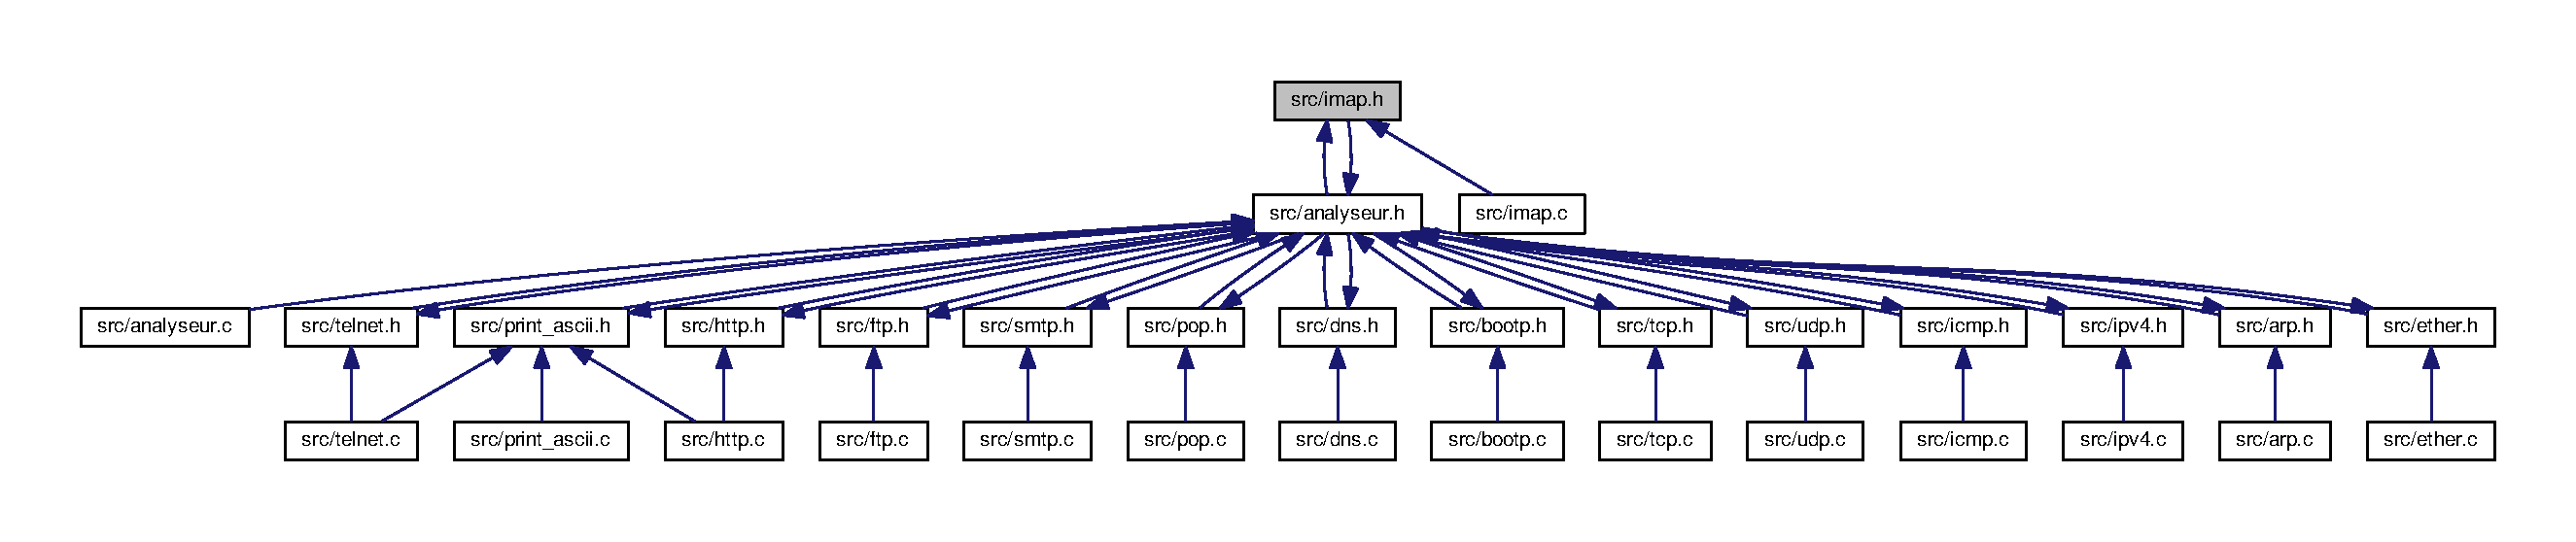
\includegraphics[width=350pt]{imap_8h__dep__incl}
\end{center}
\end{figure}
\subsection*{Functions}
\begin{DoxyCompactItemize}
\item 
void \hyperlink{imap_8h_a2f858f7da61dd47b3dc3be95f9eb2d3a}{analyse\+\_\+imap} (\hyperlink{struct_user}{User} $\ast$user, const u\+\_\+char $\ast$bytes)
\end{DoxyCompactItemize}


\subsection{Function Documentation}
\index{imap.\+h@{imap.\+h}!analyse\+\_\+imap@{analyse\+\_\+imap}}
\index{analyse\+\_\+imap@{analyse\+\_\+imap}!imap.\+h@{imap.\+h}}
\subsubsection[{\texorpdfstring{analyse\+\_\+imap(\+User $\ast$user, const u\+\_\+char $\ast$bytes)}{analyse_imap(User *user, const u_char *bytes)}}]{\setlength{\rightskip}{0pt plus 5cm}void analyse\+\_\+imap (
\begin{DoxyParamCaption}
\item[{{\bf User} $\ast$}]{user, }
\item[{const u\+\_\+char $\ast$}]{bytes}
\end{DoxyParamCaption}
)}\hypertarget{imap_8h_a2f858f7da61dd47b3dc3be95f9eb2d3a}{}\label{imap_8h_a2f858f7da61dd47b3dc3be95f9eb2d3a}

\hypertarget{ipv4_8c}{}\section{src/ipv4.c File Reference}
\label{ipv4_8c}\index{src/ipv4.\+c@{src/ipv4.\+c}}
{\ttfamily \#include \char`\"{}ipv4.\+h\char`\"{}}\\*
Include dependency graph for ipv4.\+c\+:
\nopagebreak
\begin{figure}[H]
\begin{center}
\leavevmode
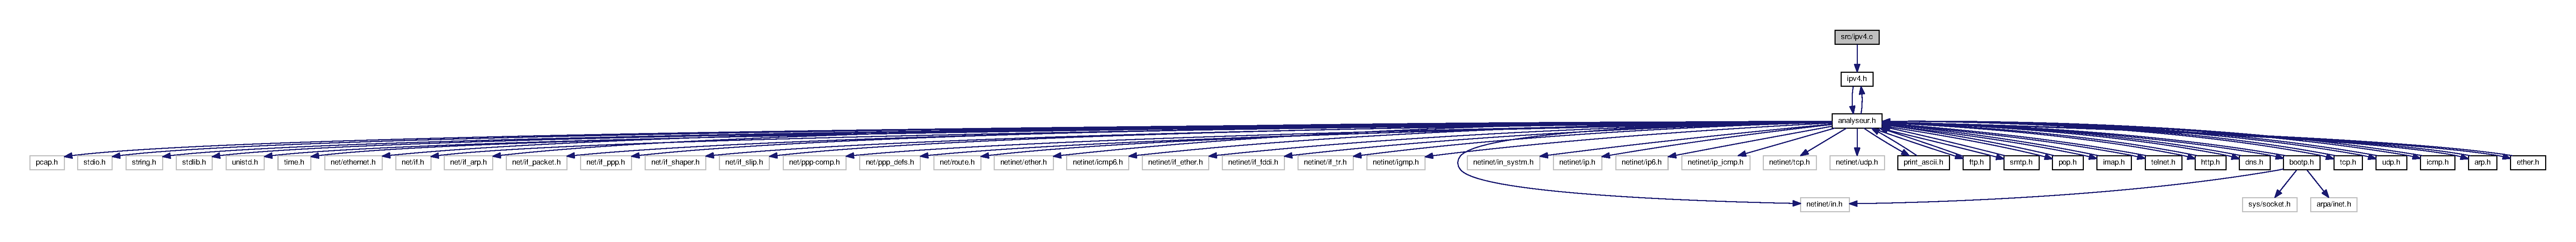
\includegraphics[width=350pt]{ipv4_8c__incl}
\end{center}
\end{figure}
\subsection*{Functions}
\begin{DoxyCompactItemize}
\item 
void \hyperlink{ipv4_8c_ae64bdfd0b989c578c4647dcd62da0626}{affichage\+\_\+ipv4} (\hyperlink{struct_user}{User} $\ast$user, \hyperlink{analyseur_8h_a6fc2e7c521fb740fdb7d8b8c16698324}{Ip\+Hdr} $\ast$iphdr)
\item 
void \hyperlink{ipv4_8c_acbe5480024782353695425fe17eebdcf}{analyse\+\_\+ipv4} (\hyperlink{struct_user}{User} $\ast$user, const u\+\_\+char $\ast$bytes)
\end{DoxyCompactItemize}


\subsection{Function Documentation}
\index{ipv4.\+c@{ipv4.\+c}!affichage\+\_\+ipv4@{affichage\+\_\+ipv4}}
\index{affichage\+\_\+ipv4@{affichage\+\_\+ipv4}!ipv4.\+c@{ipv4.\+c}}
\subsubsection[{\texorpdfstring{affichage\+\_\+ipv4(\+User $\ast$user, Ip\+Hdr $\ast$iphdr)}{affichage_ipv4(User *user, IpHdr *iphdr)}}]{\setlength{\rightskip}{0pt plus 5cm}void affichage\+\_\+ipv4 (
\begin{DoxyParamCaption}
\item[{{\bf User} $\ast$}]{user, }
\item[{{\bf Ip\+Hdr} $\ast$}]{iphdr}
\end{DoxyParamCaption}
)}\hypertarget{ipv4_8c_ae64bdfd0b989c578c4647dcd62da0626}{}\label{ipv4_8c_ae64bdfd0b989c578c4647dcd62da0626}
\index{ipv4.\+c@{ipv4.\+c}!analyse\+\_\+ipv4@{analyse\+\_\+ipv4}}
\index{analyse\+\_\+ipv4@{analyse\+\_\+ipv4}!ipv4.\+c@{ipv4.\+c}}
\subsubsection[{\texorpdfstring{analyse\+\_\+ipv4(\+User $\ast$user, const u\+\_\+char $\ast$bytes)}{analyse_ipv4(User *user, const u_char *bytes)}}]{\setlength{\rightskip}{0pt plus 5cm}void analyse\+\_\+ipv4 (
\begin{DoxyParamCaption}
\item[{{\bf User} $\ast$}]{user, }
\item[{const u\+\_\+char $\ast$}]{bytes}
\end{DoxyParamCaption}
)}\hypertarget{ipv4_8c_acbe5480024782353695425fe17eebdcf}{}\label{ipv4_8c_acbe5480024782353695425fe17eebdcf}

\hypertarget{ipv4_8h}{}\section{src/ipv4.h File Reference}
\label{ipv4_8h}\index{src/ipv4.\+h@{src/ipv4.\+h}}
{\ttfamily \#include \char`\"{}analyseur.\+h\char`\"{}}\\*
Include dependency graph for ipv4.\+h\+:
\nopagebreak
\begin{figure}[H]
\begin{center}
\leavevmode
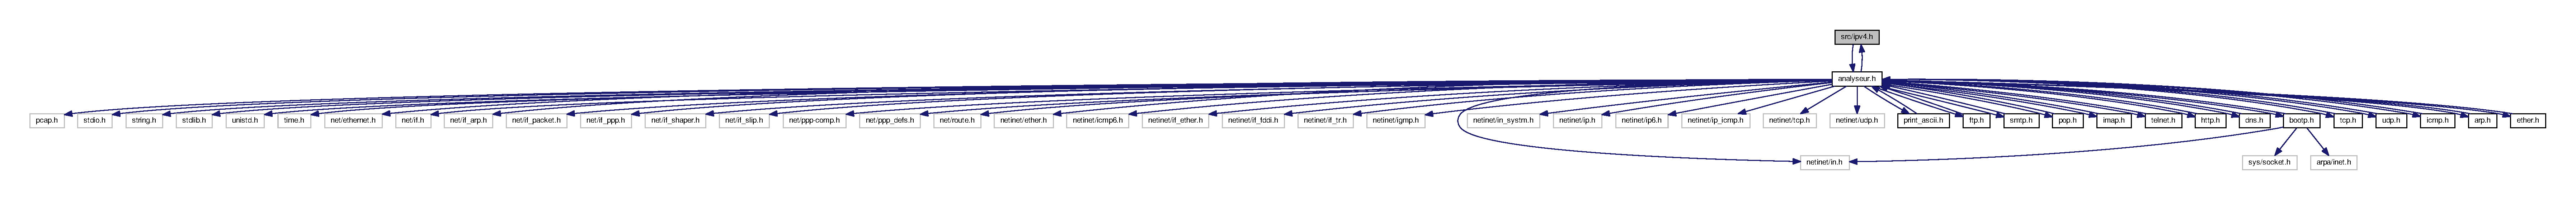
\includegraphics[width=350pt]{ipv4_8h__incl}
\end{center}
\end{figure}
This graph shows which files directly or indirectly include this file\+:
\nopagebreak
\begin{figure}[H]
\begin{center}
\leavevmode
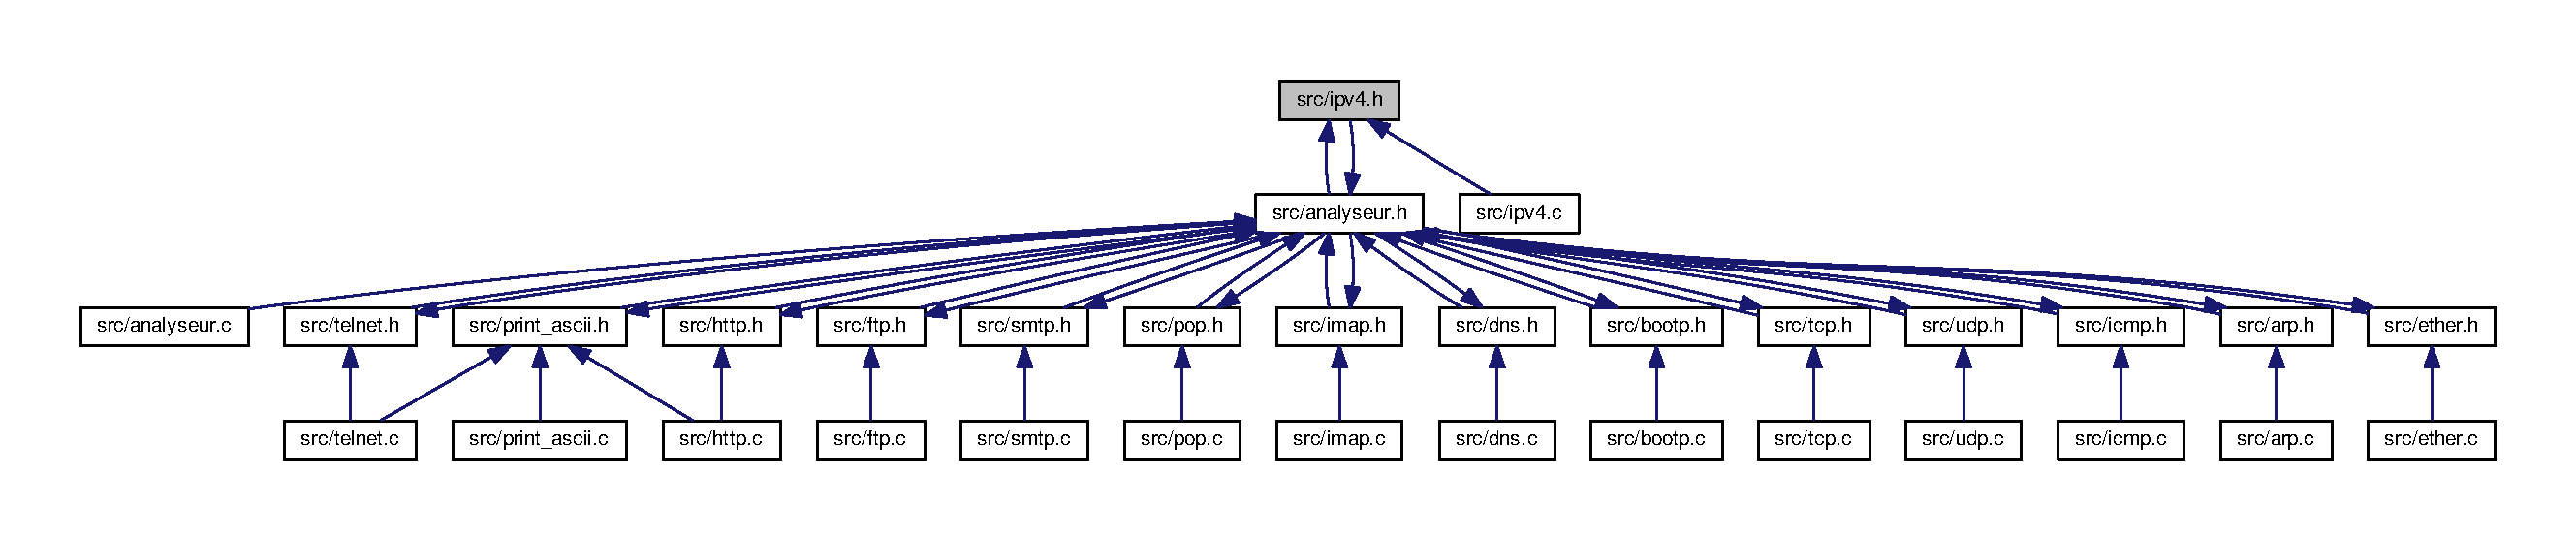
\includegraphics[width=350pt]{ipv4_8h__dep__incl}
\end{center}
\end{figure}
\subsection*{Functions}
\begin{DoxyCompactItemize}
\item 
void \hyperlink{ipv4_8h_acbe5480024782353695425fe17eebdcf}{analyse\+\_\+ipv4} (\hyperlink{struct_user}{User} $\ast$user, const u\+\_\+char $\ast$bytes)
\end{DoxyCompactItemize}


\subsection{Function Documentation}
\index{ipv4.\+h@{ipv4.\+h}!analyse\+\_\+ipv4@{analyse\+\_\+ipv4}}
\index{analyse\+\_\+ipv4@{analyse\+\_\+ipv4}!ipv4.\+h@{ipv4.\+h}}
\subsubsection[{\texorpdfstring{analyse\+\_\+ipv4(\+User $\ast$user, const u\+\_\+char $\ast$bytes)}{analyse_ipv4(User *user, const u_char *bytes)}}]{\setlength{\rightskip}{0pt plus 5cm}void analyse\+\_\+ipv4 (
\begin{DoxyParamCaption}
\item[{{\bf User} $\ast$}]{user, }
\item[{const u\+\_\+char $\ast$}]{bytes}
\end{DoxyParamCaption}
)}\hypertarget{ipv4_8h_acbe5480024782353695425fe17eebdcf}{}\label{ipv4_8h_acbe5480024782353695425fe17eebdcf}

\hypertarget{pop_8c}{}\section{src/pop.c File Reference}
\label{pop_8c}\index{src/pop.\+c@{src/pop.\+c}}
{\ttfamily \#include \char`\"{}pop.\+h\char`\"{}}\\*
Include dependency graph for pop.\+c\+:
\nopagebreak
\begin{figure}[H]
\begin{center}
\leavevmode
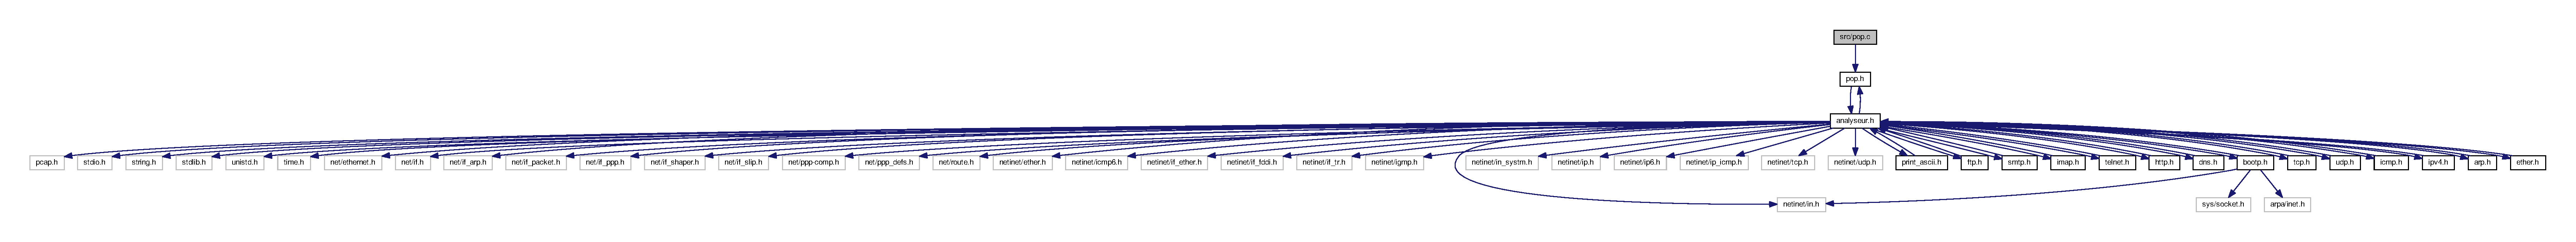
\includegraphics[width=350pt]{pop_8c__incl}
\end{center}
\end{figure}
\subsection*{Functions}
\begin{DoxyCompactItemize}
\item 
void \hyperlink{pop_8c_a6bcd27eecd3ab05cfa79b1ff2eddfd83}{affichage\+\_\+pop} (\hyperlink{struct_user}{User} $\ast$user, const u\+\_\+char $\ast$bytes)
\item 
void \hyperlink{pop_8c_aa91bf2538b3fa1ac5a6ef76b13a4103e}{analyse\+\_\+pop} (\hyperlink{struct_user}{User} $\ast$user, const u\+\_\+char $\ast$bytes)
\end{DoxyCompactItemize}


\subsection{Function Documentation}
\index{pop.\+c@{pop.\+c}!affichage\+\_\+pop@{affichage\+\_\+pop}}
\index{affichage\+\_\+pop@{affichage\+\_\+pop}!pop.\+c@{pop.\+c}}
\subsubsection[{\texorpdfstring{affichage\+\_\+pop(\+User $\ast$user, const u\+\_\+char $\ast$bytes)}{affichage_pop(User *user, const u_char *bytes)}}]{\setlength{\rightskip}{0pt plus 5cm}void affichage\+\_\+pop (
\begin{DoxyParamCaption}
\item[{{\bf User} $\ast$}]{user, }
\item[{const u\+\_\+char $\ast$}]{bytes}
\end{DoxyParamCaption}
)}\hypertarget{pop_8c_a6bcd27eecd3ab05cfa79b1ff2eddfd83}{}\label{pop_8c_a6bcd27eecd3ab05cfa79b1ff2eddfd83}
\index{pop.\+c@{pop.\+c}!analyse\+\_\+pop@{analyse\+\_\+pop}}
\index{analyse\+\_\+pop@{analyse\+\_\+pop}!pop.\+c@{pop.\+c}}
\subsubsection[{\texorpdfstring{analyse\+\_\+pop(\+User $\ast$user, const u\+\_\+char $\ast$bytes)}{analyse_pop(User *user, const u_char *bytes)}}]{\setlength{\rightskip}{0pt plus 5cm}void analyse\+\_\+pop (
\begin{DoxyParamCaption}
\item[{{\bf User} $\ast$}]{user, }
\item[{const u\+\_\+char $\ast$}]{bytes}
\end{DoxyParamCaption}
)}\hypertarget{pop_8c_aa91bf2538b3fa1ac5a6ef76b13a4103e}{}\label{pop_8c_aa91bf2538b3fa1ac5a6ef76b13a4103e}

\hypertarget{pop_8h}{}\section{src/pop.h File Reference}
\label{pop_8h}\index{src/pop.\+h@{src/pop.\+h}}
{\ttfamily \#include \char`\"{}analyseur.\+h\char`\"{}}\\*
Include dependency graph for pop.\+h\+:
\nopagebreak
\begin{figure}[H]
\begin{center}
\leavevmode
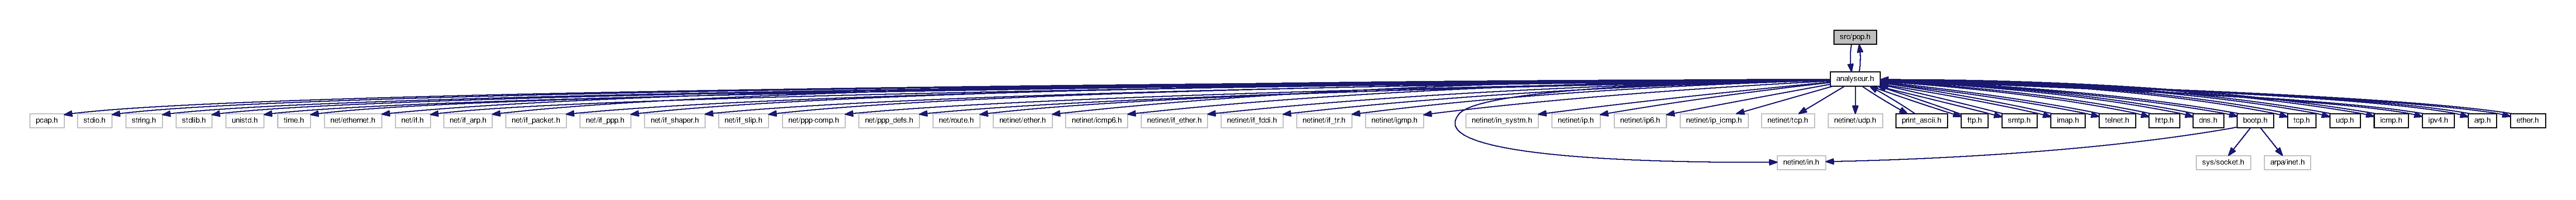
\includegraphics[width=350pt]{pop_8h__incl}
\end{center}
\end{figure}
This graph shows which files directly or indirectly include this file\+:
\nopagebreak
\begin{figure}[H]
\begin{center}
\leavevmode
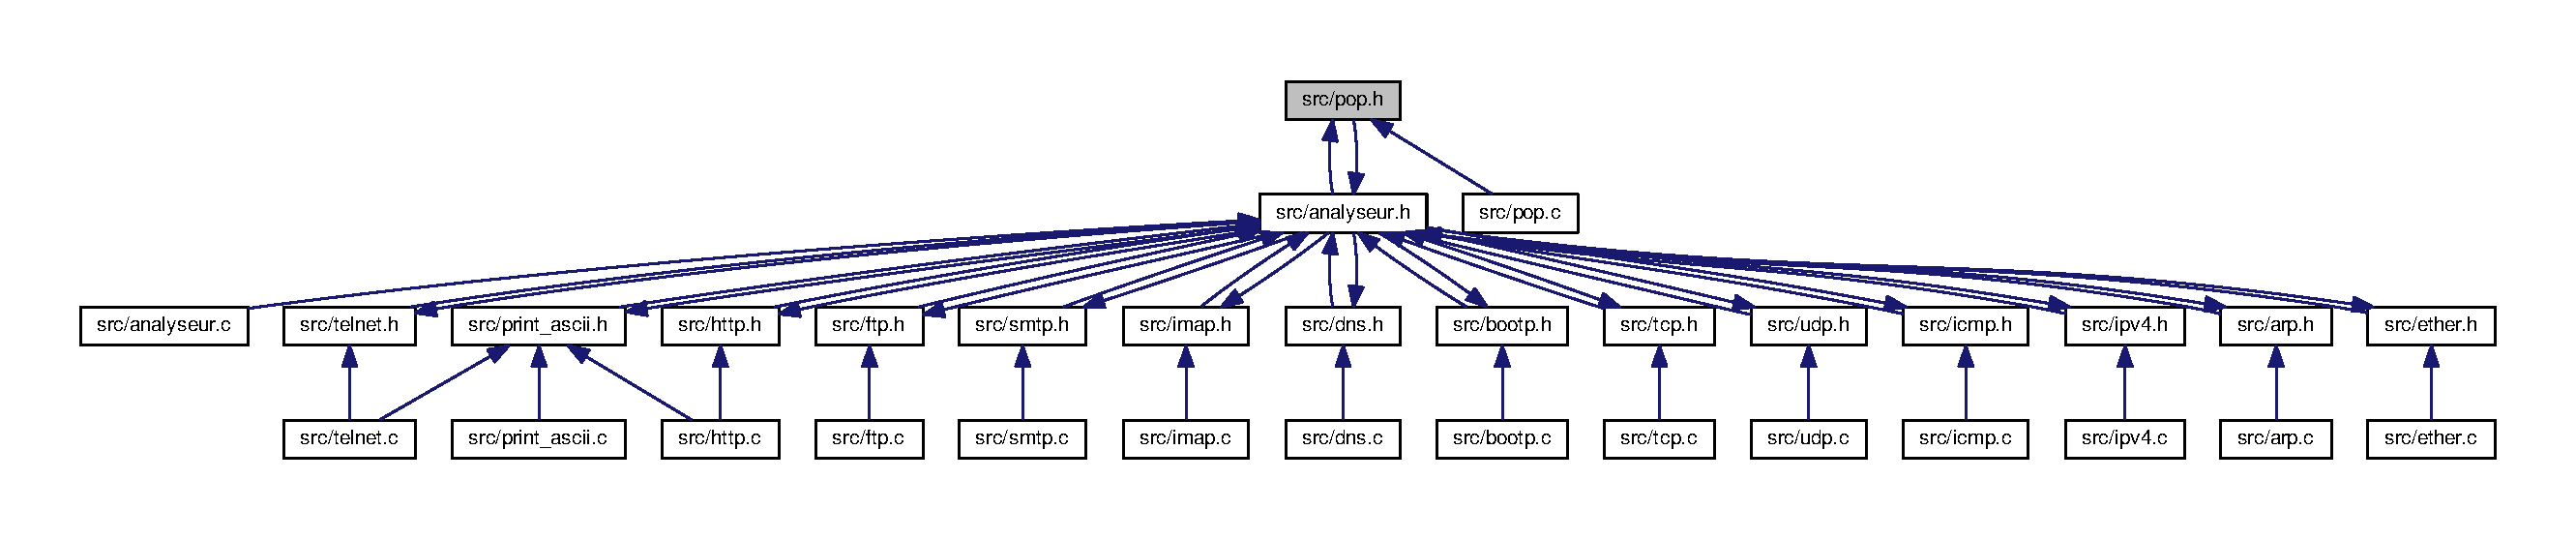
\includegraphics[width=350pt]{pop_8h__dep__incl}
\end{center}
\end{figure}
\subsection*{Functions}
\begin{DoxyCompactItemize}
\item 
void \hyperlink{pop_8h_aa91bf2538b3fa1ac5a6ef76b13a4103e}{analyse\+\_\+pop} (\hyperlink{struct_user}{User} $\ast$user, const u\+\_\+char $\ast$bytes)
\end{DoxyCompactItemize}


\subsection{Function Documentation}
\index{pop.\+h@{pop.\+h}!analyse\+\_\+pop@{analyse\+\_\+pop}}
\index{analyse\+\_\+pop@{analyse\+\_\+pop}!pop.\+h@{pop.\+h}}
\subsubsection[{\texorpdfstring{analyse\+\_\+pop(\+User $\ast$user, const u\+\_\+char $\ast$bytes)}{analyse_pop(User *user, const u_char *bytes)}}]{\setlength{\rightskip}{0pt plus 5cm}void analyse\+\_\+pop (
\begin{DoxyParamCaption}
\item[{{\bf User} $\ast$}]{user, }
\item[{const u\+\_\+char $\ast$}]{bytes}
\end{DoxyParamCaption}
)}\hypertarget{pop_8h_aa91bf2538b3fa1ac5a6ef76b13a4103e}{}\label{pop_8h_aa91bf2538b3fa1ac5a6ef76b13a4103e}

\hypertarget{print__ascii_8c}{}\section{src/print\+\_\+ascii.c File Reference}
\label{print__ascii_8c}\index{src/print\+\_\+ascii.\+c@{src/print\+\_\+ascii.\+c}}
{\ttfamily \#include \char`\"{}print\+\_\+ascii.\+h\char`\"{}}\\*
{\ttfamily \#include $<$ctype.\+h$>$}\\*
Include dependency graph for print\+\_\+ascii.\+c\+:
\nopagebreak
\begin{figure}[H]
\begin{center}
\leavevmode
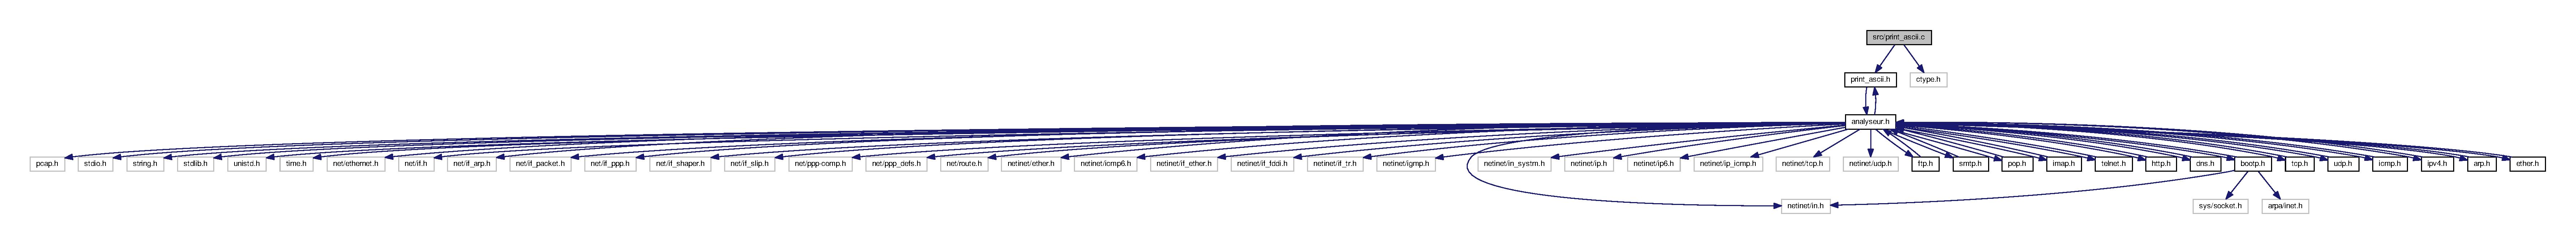
\includegraphics[width=350pt]{print__ascii_8c__incl}
\end{center}
\end{figure}
\subsection*{Functions}
\begin{DoxyCompactItemize}
\item 
void \hyperlink{print__ascii_8c_a4b40892442012ecd46859a4c8a789b15}{print\+\_\+ascii\+\_\+line\+\_\+len} (\hyperlink{struct_user}{User} $\ast$user, const u\+\_\+char $\ast$payload, int len)
\item 
void \hyperlink{print__ascii_8c_a43fa30287f1d59a23326b47204fb8999}{print\+\_\+hex\+\_\+ascii\+\_\+line} (\hyperlink{struct_user}{User} $\ast$user, const u\+\_\+char $\ast$payload)
\end{DoxyCompactItemize}


\subsection{Function Documentation}
\index{print\+\_\+ascii.\+c@{print\+\_\+ascii.\+c}!print\+\_\+ascii\+\_\+line\+\_\+len@{print\+\_\+ascii\+\_\+line\+\_\+len}}
\index{print\+\_\+ascii\+\_\+line\+\_\+len@{print\+\_\+ascii\+\_\+line\+\_\+len}!print\+\_\+ascii.\+c@{print\+\_\+ascii.\+c}}
\subsubsection[{\texorpdfstring{print\+\_\+ascii\+\_\+line\+\_\+len(\+User $\ast$user, const u\+\_\+char $\ast$payload, int len)}{print_ascii_line_len(User *user, const u_char *payload, int len)}}]{\setlength{\rightskip}{0pt plus 5cm}void print\+\_\+ascii\+\_\+line\+\_\+len (
\begin{DoxyParamCaption}
\item[{{\bf User} $\ast$}]{user, }
\item[{const u\+\_\+char $\ast$}]{payload, }
\item[{int}]{len}
\end{DoxyParamCaption}
)}\hypertarget{print__ascii_8c_a4b40892442012ecd46859a4c8a789b15}{}\label{print__ascii_8c_a4b40892442012ecd46859a4c8a789b15}
\index{print\+\_\+ascii.\+c@{print\+\_\+ascii.\+c}!print\+\_\+hex\+\_\+ascii\+\_\+line@{print\+\_\+hex\+\_\+ascii\+\_\+line}}
\index{print\+\_\+hex\+\_\+ascii\+\_\+line@{print\+\_\+hex\+\_\+ascii\+\_\+line}!print\+\_\+ascii.\+c@{print\+\_\+ascii.\+c}}
\subsubsection[{\texorpdfstring{print\+\_\+hex\+\_\+ascii\+\_\+line(\+User $\ast$user, const u\+\_\+char $\ast$payload)}{print_hex_ascii_line(User *user, const u_char *payload)}}]{\setlength{\rightskip}{0pt plus 5cm}void print\+\_\+hex\+\_\+ascii\+\_\+line (
\begin{DoxyParamCaption}
\item[{{\bf User} $\ast$}]{user, }
\item[{const u\+\_\+char $\ast$}]{payload}
\end{DoxyParamCaption}
)}\hypertarget{print__ascii_8c_a43fa30287f1d59a23326b47204fb8999}{}\label{print__ascii_8c_a43fa30287f1d59a23326b47204fb8999}

\hypertarget{print__ascii_8h}{}\section{src/print\+\_\+ascii.h File Reference}
\label{print__ascii_8h}\index{src/print\+\_\+ascii.\+h@{src/print\+\_\+ascii.\+h}}
{\ttfamily \#include \char`\"{}analyseur.\+h\char`\"{}}\\*
Include dependency graph for print\+\_\+ascii.\+h\+:
\nopagebreak
\begin{figure}[H]
\begin{center}
\leavevmode
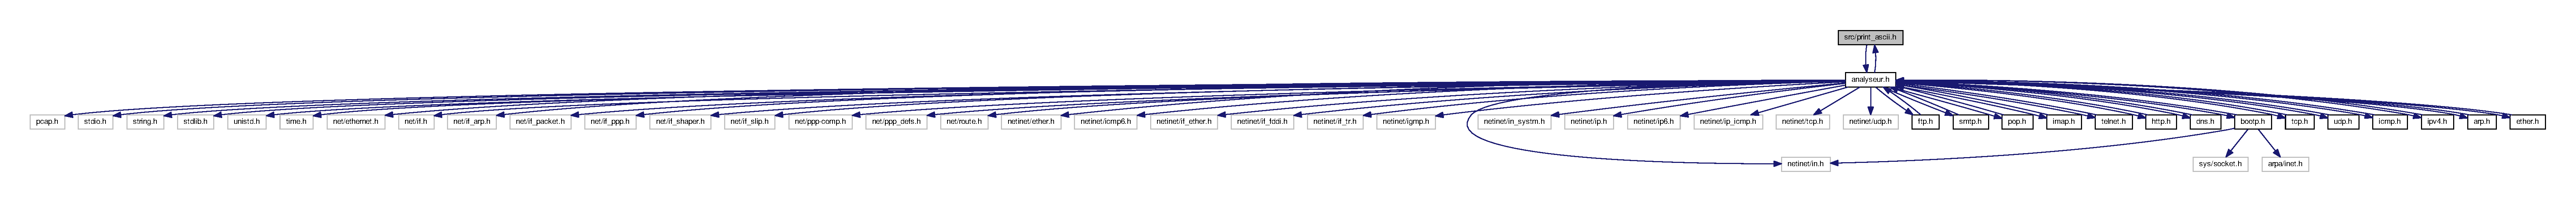
\includegraphics[width=350pt]{print__ascii_8h__incl}
\end{center}
\end{figure}
This graph shows which files directly or indirectly include this file\+:
\nopagebreak
\begin{figure}[H]
\begin{center}
\leavevmode
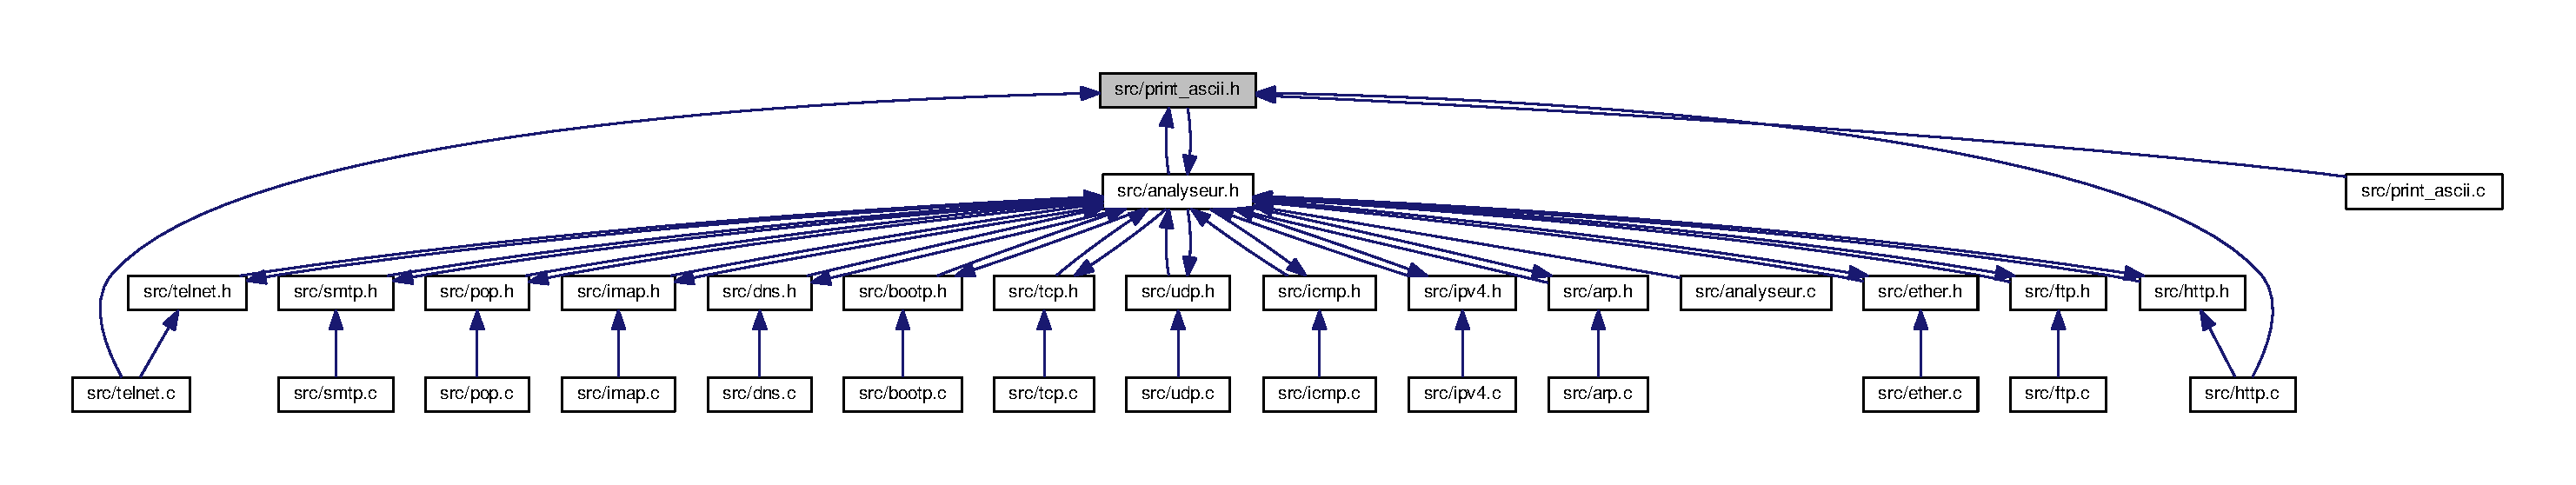
\includegraphics[width=350pt]{print__ascii_8h__dep__incl}
\end{center}
\end{figure}
\subsection*{Functions}
\begin{DoxyCompactItemize}
\item 
void \hyperlink{print__ascii_8h_a4b40892442012ecd46859a4c8a789b15}{print\+\_\+ascii\+\_\+line\+\_\+len} (\hyperlink{struct_user}{User} $\ast$user, const u\+\_\+char $\ast$payload, int len)
\item 
void \hyperlink{print__ascii_8h_a43fa30287f1d59a23326b47204fb8999}{print\+\_\+hex\+\_\+ascii\+\_\+line} (\hyperlink{struct_user}{User} $\ast$user, const u\+\_\+char $\ast$payload)
\end{DoxyCompactItemize}


\subsection{Function Documentation}
\index{print\+\_\+ascii.\+h@{print\+\_\+ascii.\+h}!print\+\_\+ascii\+\_\+line\+\_\+len@{print\+\_\+ascii\+\_\+line\+\_\+len}}
\index{print\+\_\+ascii\+\_\+line\+\_\+len@{print\+\_\+ascii\+\_\+line\+\_\+len}!print\+\_\+ascii.\+h@{print\+\_\+ascii.\+h}}
\subsubsection[{\texorpdfstring{print\+\_\+ascii\+\_\+line\+\_\+len(\+User $\ast$user, const u\+\_\+char $\ast$payload, int len)}{print_ascii_line_len(User *user, const u_char *payload, int len)}}]{\setlength{\rightskip}{0pt plus 5cm}void print\+\_\+ascii\+\_\+line\+\_\+len (
\begin{DoxyParamCaption}
\item[{{\bf User} $\ast$}]{user, }
\item[{const u\+\_\+char $\ast$}]{payload, }
\item[{int}]{len}
\end{DoxyParamCaption}
)}\hypertarget{print__ascii_8h_a4b40892442012ecd46859a4c8a789b15}{}\label{print__ascii_8h_a4b40892442012ecd46859a4c8a789b15}
\index{print\+\_\+ascii.\+h@{print\+\_\+ascii.\+h}!print\+\_\+hex\+\_\+ascii\+\_\+line@{print\+\_\+hex\+\_\+ascii\+\_\+line}}
\index{print\+\_\+hex\+\_\+ascii\+\_\+line@{print\+\_\+hex\+\_\+ascii\+\_\+line}!print\+\_\+ascii.\+h@{print\+\_\+ascii.\+h}}
\subsubsection[{\texorpdfstring{print\+\_\+hex\+\_\+ascii\+\_\+line(\+User $\ast$user, const u\+\_\+char $\ast$payload)}{print_hex_ascii_line(User *user, const u_char *payload)}}]{\setlength{\rightskip}{0pt plus 5cm}void print\+\_\+hex\+\_\+ascii\+\_\+line (
\begin{DoxyParamCaption}
\item[{{\bf User} $\ast$}]{user, }
\item[{const u\+\_\+char $\ast$}]{payload}
\end{DoxyParamCaption}
)}\hypertarget{print__ascii_8h_a43fa30287f1d59a23326b47204fb8999}{}\label{print__ascii_8h_a43fa30287f1d59a23326b47204fb8999}

\hypertarget{smtp_8c}{}\section{src/smtp.c File Reference}
\label{smtp_8c}\index{src/smtp.\+c@{src/smtp.\+c}}
{\ttfamily \#include \char`\"{}smtp.\+h\char`\"{}}\\*
Include dependency graph for smtp.\+c\+:
\nopagebreak
\begin{figure}[H]
\begin{center}
\leavevmode
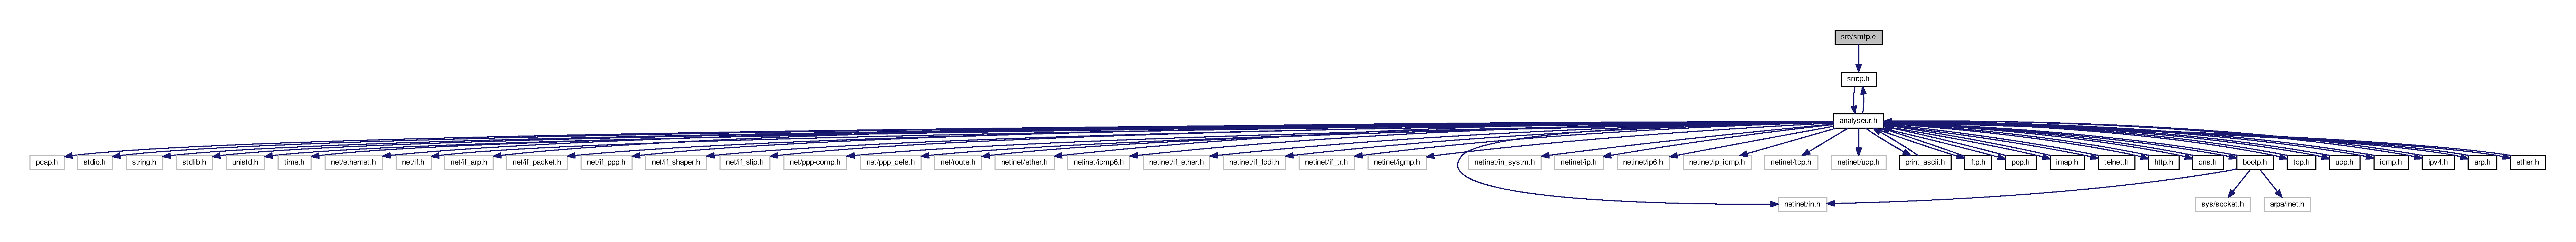
\includegraphics[width=350pt]{smtp_8c__incl}
\end{center}
\end{figure}
\subsection*{Functions}
\begin{DoxyCompactItemize}
\item 
void \hyperlink{smtp_8c_a692c5725d4596c78f97188918eedb62f}{affichage\+\_\+smtp} (\hyperlink{struct_user}{User} $\ast$user, const u\+\_\+char $\ast$bytes)
\item 
void \hyperlink{smtp_8c_ad51aefc6b3d1fcaaf48e73f4bb7cd54e}{analyse\+\_\+smtp} (\hyperlink{struct_user}{User} $\ast$user, const u\+\_\+char $\ast$bytes)
\end{DoxyCompactItemize}


\subsection{Function Documentation}
\index{smtp.\+c@{smtp.\+c}!affichage\+\_\+smtp@{affichage\+\_\+smtp}}
\index{affichage\+\_\+smtp@{affichage\+\_\+smtp}!smtp.\+c@{smtp.\+c}}
\subsubsection[{\texorpdfstring{affichage\+\_\+smtp(\+User $\ast$user, const u\+\_\+char $\ast$bytes)}{affichage_smtp(User *user, const u_char *bytes)}}]{\setlength{\rightskip}{0pt plus 5cm}void affichage\+\_\+smtp (
\begin{DoxyParamCaption}
\item[{{\bf User} $\ast$}]{user, }
\item[{const u\+\_\+char $\ast$}]{bytes}
\end{DoxyParamCaption}
)}\hypertarget{smtp_8c_a692c5725d4596c78f97188918eedb62f}{}\label{smtp_8c_a692c5725d4596c78f97188918eedb62f}
\index{smtp.\+c@{smtp.\+c}!analyse\+\_\+smtp@{analyse\+\_\+smtp}}
\index{analyse\+\_\+smtp@{analyse\+\_\+smtp}!smtp.\+c@{smtp.\+c}}
\subsubsection[{\texorpdfstring{analyse\+\_\+smtp(\+User $\ast$user, const u\+\_\+char $\ast$bytes)}{analyse_smtp(User *user, const u_char *bytes)}}]{\setlength{\rightskip}{0pt plus 5cm}void analyse\+\_\+smtp (
\begin{DoxyParamCaption}
\item[{{\bf User} $\ast$}]{user, }
\item[{const u\+\_\+char $\ast$}]{bytes}
\end{DoxyParamCaption}
)}\hypertarget{smtp_8c_ad51aefc6b3d1fcaaf48e73f4bb7cd54e}{}\label{smtp_8c_ad51aefc6b3d1fcaaf48e73f4bb7cd54e}

\hypertarget{smtp_8h}{}\section{src/smtp.h File Reference}
\label{smtp_8h}\index{src/smtp.\+h@{src/smtp.\+h}}
{\ttfamily \#include \char`\"{}analyseur.\+h\char`\"{}}\\*
Include dependency graph for smtp.\+h\+:
\nopagebreak
\begin{figure}[H]
\begin{center}
\leavevmode
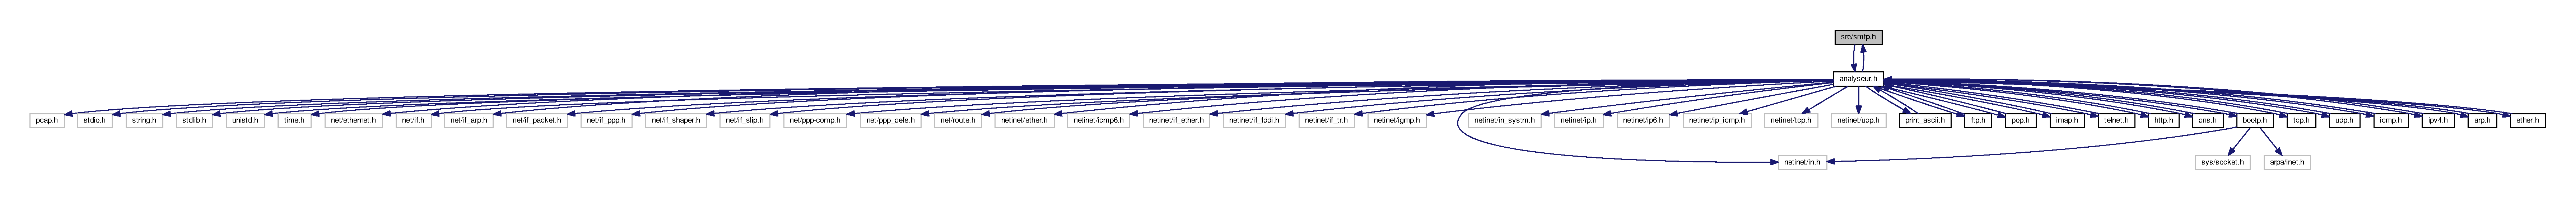
\includegraphics[width=350pt]{smtp_8h__incl}
\end{center}
\end{figure}
This graph shows which files directly or indirectly include this file\+:
\nopagebreak
\begin{figure}[H]
\begin{center}
\leavevmode
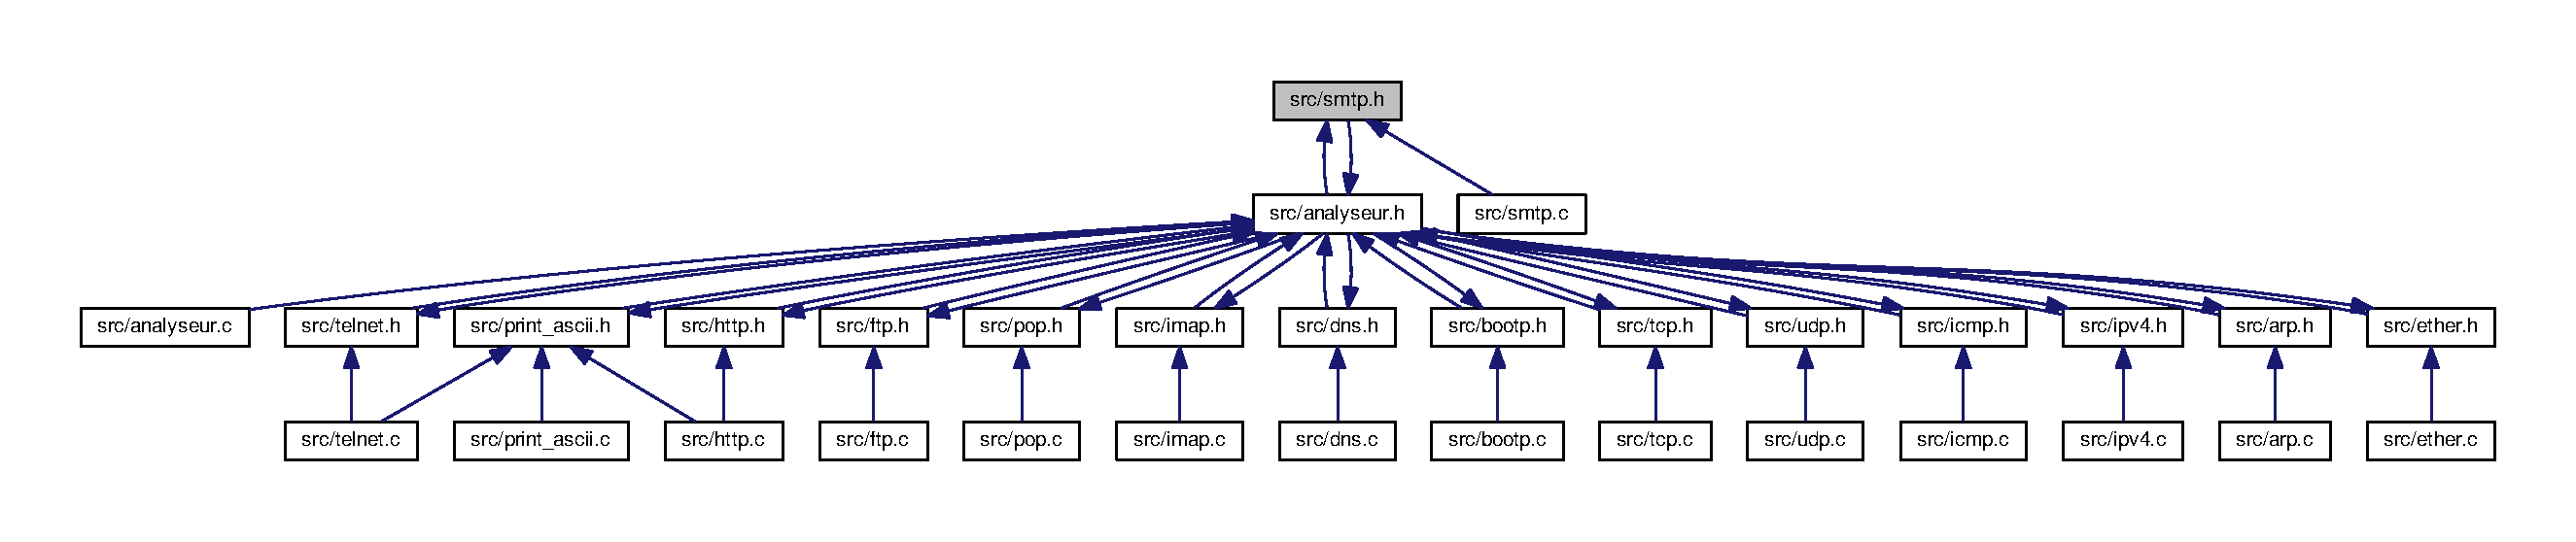
\includegraphics[width=350pt]{smtp_8h__dep__incl}
\end{center}
\end{figure}
\subsection*{Functions}
\begin{DoxyCompactItemize}
\item 
void \hyperlink{smtp_8h_ad51aefc6b3d1fcaaf48e73f4bb7cd54e}{analyse\+\_\+smtp} (\hyperlink{struct_user}{User} $\ast$user, const u\+\_\+char $\ast$bytes)
\end{DoxyCompactItemize}


\subsection{Function Documentation}
\index{smtp.\+h@{smtp.\+h}!analyse\+\_\+smtp@{analyse\+\_\+smtp}}
\index{analyse\+\_\+smtp@{analyse\+\_\+smtp}!smtp.\+h@{smtp.\+h}}
\subsubsection[{\texorpdfstring{analyse\+\_\+smtp(\+User $\ast$user, const u\+\_\+char $\ast$bytes)}{analyse_smtp(User *user, const u_char *bytes)}}]{\setlength{\rightskip}{0pt plus 5cm}void analyse\+\_\+smtp (
\begin{DoxyParamCaption}
\item[{{\bf User} $\ast$}]{user, }
\item[{const u\+\_\+char $\ast$}]{bytes}
\end{DoxyParamCaption}
)}\hypertarget{smtp_8h_ad51aefc6b3d1fcaaf48e73f4bb7cd54e}{}\label{smtp_8h_ad51aefc6b3d1fcaaf48e73f4bb7cd54e}

\hypertarget{tcp_8c}{}\section{src/tcp.c File Reference}
\label{tcp_8c}\index{src/tcp.\+c@{src/tcp.\+c}}
{\ttfamily \#include \char`\"{}tcp.\+h\char`\"{}}\\*
Include dependency graph for tcp.\+c\+:
\nopagebreak
\begin{figure}[H]
\begin{center}
\leavevmode
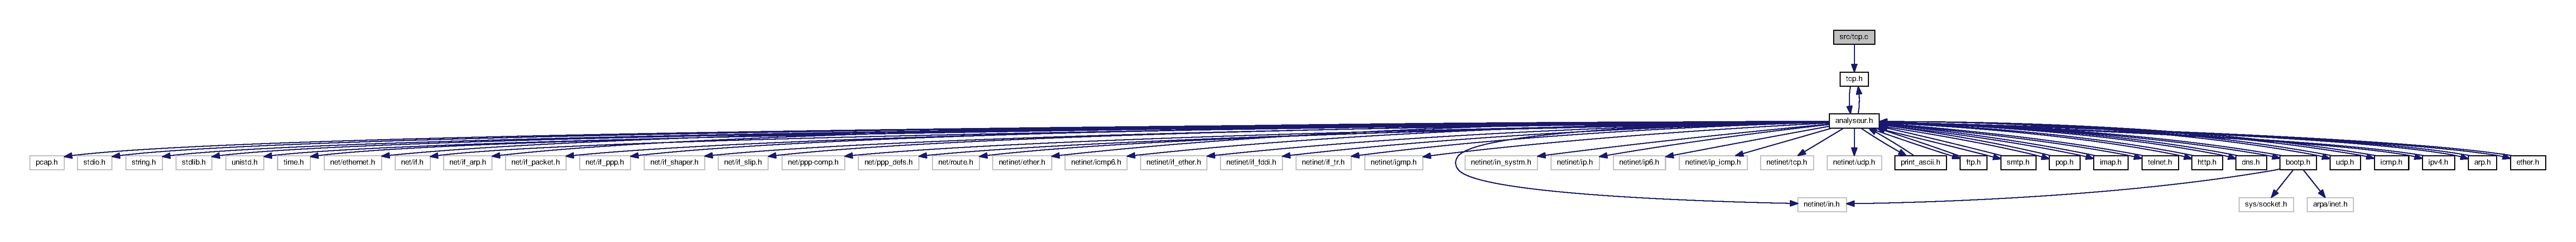
\includegraphics[width=350pt]{tcp_8c__incl}
\end{center}
\end{figure}
\subsection*{Functions}
\begin{DoxyCompactItemize}
\item 
void \hyperlink{tcp_8c_ac060ce0452afbb1832c6621ed1fa02ce}{affichage\+\_\+tcp} (\hyperlink{struct_user}{User} $\ast$user, \hyperlink{analyseur_8h_a0a79f5959e54cfe5f13ff5207c59152e}{Tcp\+Hdr} $\ast$h)
\item 
void \hyperlink{tcp_8c_a20ef791b899f1d26c49f0f661142b52d}{analyse\+\_\+tcp} (\hyperlink{struct_user}{User} $\ast$user, const u\+\_\+char $\ast$bytes)
\end{DoxyCompactItemize}


\subsection{Function Documentation}
\index{tcp.\+c@{tcp.\+c}!affichage\+\_\+tcp@{affichage\+\_\+tcp}}
\index{affichage\+\_\+tcp@{affichage\+\_\+tcp}!tcp.\+c@{tcp.\+c}}
\subsubsection[{\texorpdfstring{affichage\+\_\+tcp(\+User $\ast$user, Tcp\+Hdr $\ast$h)}{affichage_tcp(User *user, TcpHdr *h)}}]{\setlength{\rightskip}{0pt plus 5cm}void affichage\+\_\+tcp (
\begin{DoxyParamCaption}
\item[{{\bf User} $\ast$}]{user, }
\item[{{\bf Tcp\+Hdr} $\ast$}]{h}
\end{DoxyParamCaption}
)}\hypertarget{tcp_8c_ac060ce0452afbb1832c6621ed1fa02ce}{}\label{tcp_8c_ac060ce0452afbb1832c6621ed1fa02ce}
\index{tcp.\+c@{tcp.\+c}!analyse\+\_\+tcp@{analyse\+\_\+tcp}}
\index{analyse\+\_\+tcp@{analyse\+\_\+tcp}!tcp.\+c@{tcp.\+c}}
\subsubsection[{\texorpdfstring{analyse\+\_\+tcp(\+User $\ast$user, const u\+\_\+char $\ast$bytes)}{analyse_tcp(User *user, const u_char *bytes)}}]{\setlength{\rightskip}{0pt plus 5cm}void analyse\+\_\+tcp (
\begin{DoxyParamCaption}
\item[{{\bf User} $\ast$}]{user, }
\item[{const u\+\_\+char $\ast$}]{bytes}
\end{DoxyParamCaption}
)}\hypertarget{tcp_8c_a20ef791b899f1d26c49f0f661142b52d}{}\label{tcp_8c_a20ef791b899f1d26c49f0f661142b52d}

\hypertarget{tcp_8h}{}\section{src/tcp.h File Reference}
\label{tcp_8h}\index{src/tcp.\+h@{src/tcp.\+h}}
{\ttfamily \#include \char`\"{}analyseur.\+h\char`\"{}}\\*
Include dependency graph for tcp.\+h\+:
\nopagebreak
\begin{figure}[H]
\begin{center}
\leavevmode
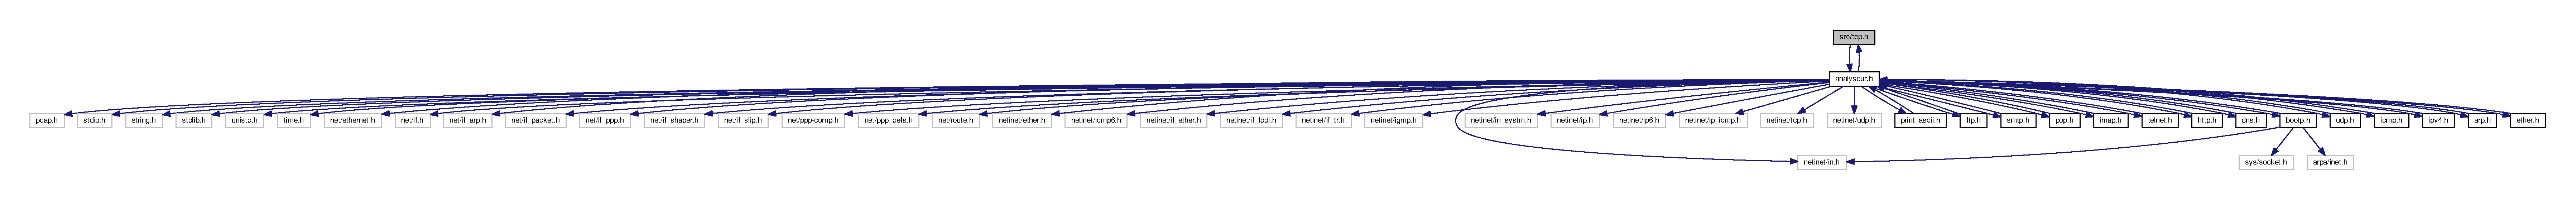
\includegraphics[width=350pt]{tcp_8h__incl}
\end{center}
\end{figure}
This graph shows which files directly or indirectly include this file\+:
\nopagebreak
\begin{figure}[H]
\begin{center}
\leavevmode
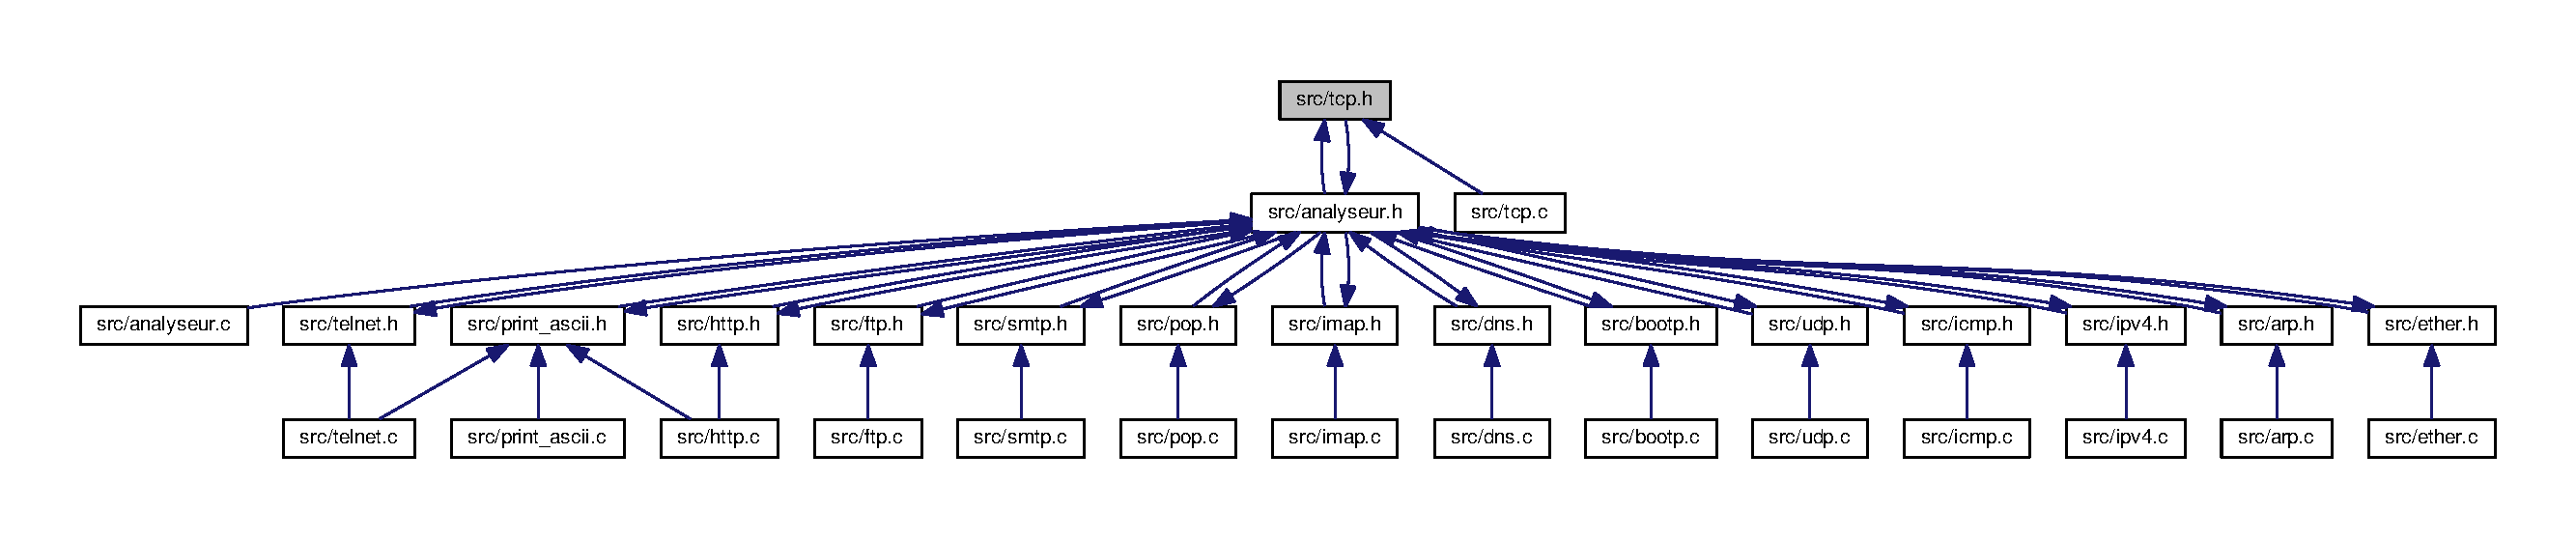
\includegraphics[width=350pt]{tcp_8h__dep__incl}
\end{center}
\end{figure}
\subsection*{Functions}
\begin{DoxyCompactItemize}
\item 
void \hyperlink{tcp_8h_a20ef791b899f1d26c49f0f661142b52d}{analyse\+\_\+tcp} (\hyperlink{struct_user}{User} $\ast$user, const u\+\_\+char $\ast$bytes)
\end{DoxyCompactItemize}


\subsection{Function Documentation}
\index{tcp.\+h@{tcp.\+h}!analyse\+\_\+tcp@{analyse\+\_\+tcp}}
\index{analyse\+\_\+tcp@{analyse\+\_\+tcp}!tcp.\+h@{tcp.\+h}}
\subsubsection[{\texorpdfstring{analyse\+\_\+tcp(\+User $\ast$user, const u\+\_\+char $\ast$bytes)}{analyse_tcp(User *user, const u_char *bytes)}}]{\setlength{\rightskip}{0pt plus 5cm}void analyse\+\_\+tcp (
\begin{DoxyParamCaption}
\item[{{\bf User} $\ast$}]{user, }
\item[{const u\+\_\+char $\ast$}]{bytes}
\end{DoxyParamCaption}
)}\hypertarget{tcp_8h_a20ef791b899f1d26c49f0f661142b52d}{}\label{tcp_8h_a20ef791b899f1d26c49f0f661142b52d}

\hypertarget{telnet_8c}{}\section{src/telnet.c File Reference}
\label{telnet_8c}\index{src/telnet.\+c@{src/telnet.\+c}}
{\ttfamily \#include \char`\"{}telnet.\+h\char`\"{}}\\*
{\ttfamily \#include \char`\"{}print\+\_\+ascii.\+h\char`\"{}}\\*
Include dependency graph for telnet.\+c\+:
\nopagebreak
\begin{figure}[H]
\begin{center}
\leavevmode
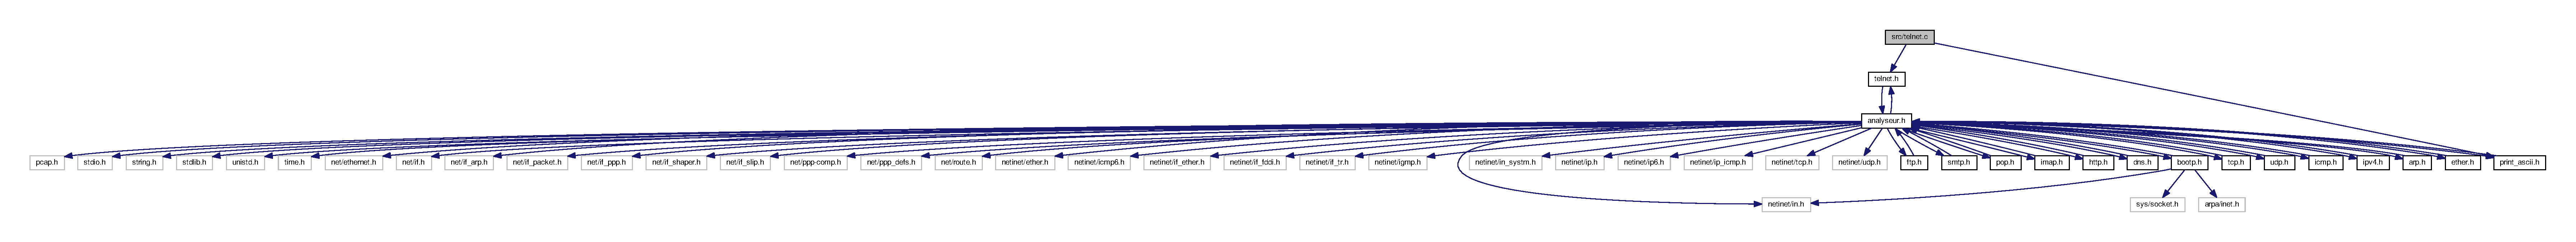
\includegraphics[width=350pt]{telnet_8c__incl}
\end{center}
\end{figure}
\subsection*{Functions}
\begin{DoxyCompactItemize}
\item 
void \hyperlink{telnet_8c_a8de49f6269be15ab2b8fb3eb0710421e}{affichage\+\_\+telnet} (\hyperlink{struct_user}{User} $\ast$user, const u\+\_\+char $\ast$bytes)
\item 
void \hyperlink{telnet_8c_a2feb0b35b5ca7a20559919c9d55797ff}{analyse\+\_\+telnet} (\hyperlink{struct_user}{User} $\ast$user, const u\+\_\+char $\ast$bytes)
\end{DoxyCompactItemize}


\subsection{Function Documentation}
\index{telnet.\+c@{telnet.\+c}!affichage\+\_\+telnet@{affichage\+\_\+telnet}}
\index{affichage\+\_\+telnet@{affichage\+\_\+telnet}!telnet.\+c@{telnet.\+c}}
\subsubsection[{\texorpdfstring{affichage\+\_\+telnet(\+User $\ast$user, const u\+\_\+char $\ast$bytes)}{affichage_telnet(User *user, const u_char *bytes)}}]{\setlength{\rightskip}{0pt plus 5cm}void affichage\+\_\+telnet (
\begin{DoxyParamCaption}
\item[{{\bf User} $\ast$}]{user, }
\item[{const u\+\_\+char $\ast$}]{bytes}
\end{DoxyParamCaption}
)}\hypertarget{telnet_8c_a8de49f6269be15ab2b8fb3eb0710421e}{}\label{telnet_8c_a8de49f6269be15ab2b8fb3eb0710421e}
\index{telnet.\+c@{telnet.\+c}!analyse\+\_\+telnet@{analyse\+\_\+telnet}}
\index{analyse\+\_\+telnet@{analyse\+\_\+telnet}!telnet.\+c@{telnet.\+c}}
\subsubsection[{\texorpdfstring{analyse\+\_\+telnet(\+User $\ast$user, const u\+\_\+char $\ast$bytes)}{analyse_telnet(User *user, const u_char *bytes)}}]{\setlength{\rightskip}{0pt plus 5cm}void analyse\+\_\+telnet (
\begin{DoxyParamCaption}
\item[{{\bf User} $\ast$}]{user, }
\item[{const u\+\_\+char $\ast$}]{bytes}
\end{DoxyParamCaption}
)}\hypertarget{telnet_8c_a2feb0b35b5ca7a20559919c9d55797ff}{}\label{telnet_8c_a2feb0b35b5ca7a20559919c9d55797ff}

\hypertarget{telnet_8h}{}\section{src/telnet.h File Reference}
\label{telnet_8h}\index{src/telnet.\+h@{src/telnet.\+h}}
{\ttfamily \#include \char`\"{}analyseur.\+h\char`\"{}}\\*
Include dependency graph for telnet.\+h\+:
\nopagebreak
\begin{figure}[H]
\begin{center}
\leavevmode
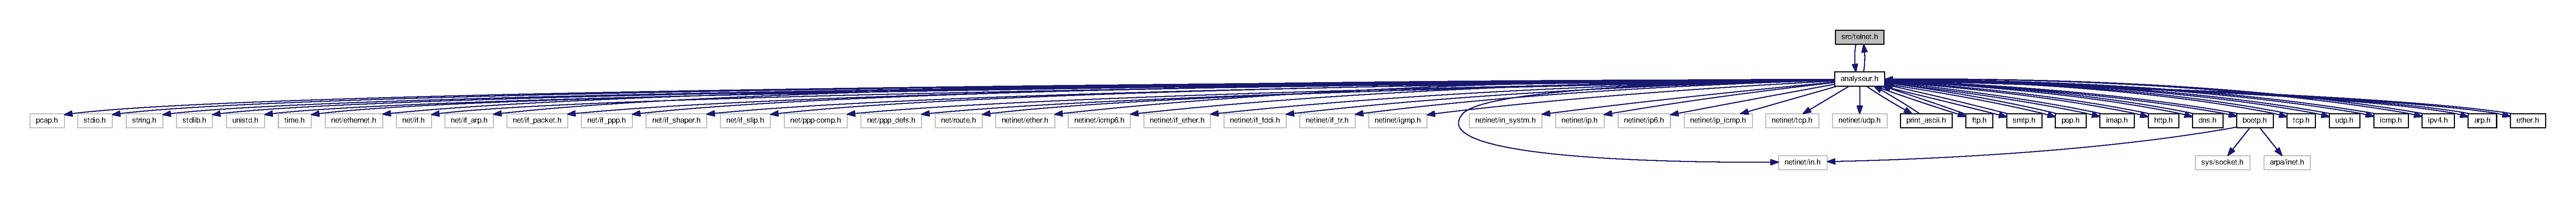
\includegraphics[width=350pt]{telnet_8h__incl}
\end{center}
\end{figure}
This graph shows which files directly or indirectly include this file\+:
\nopagebreak
\begin{figure}[H]
\begin{center}
\leavevmode
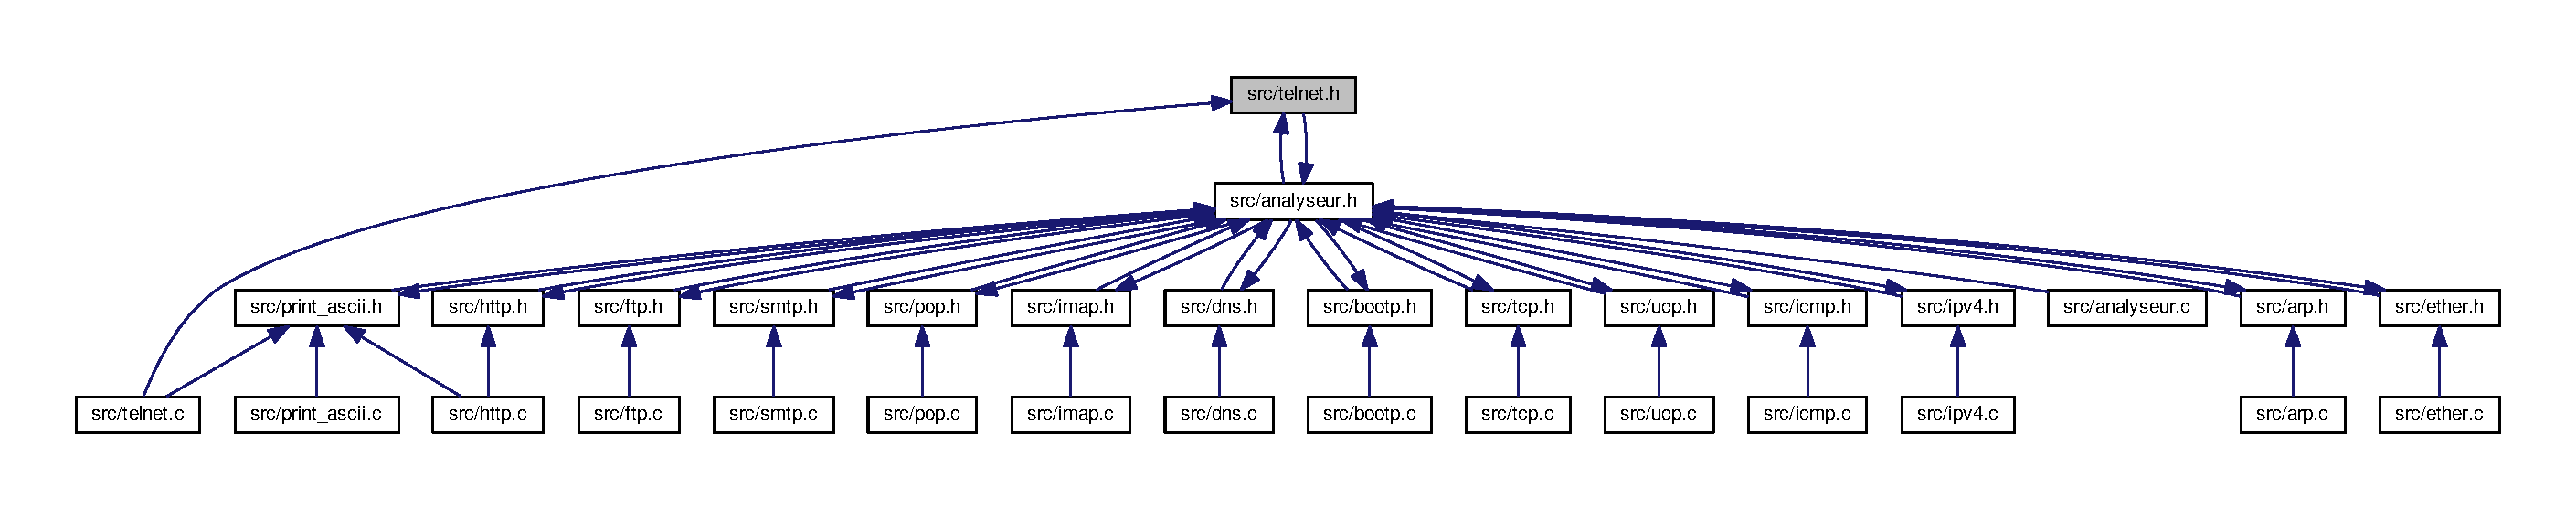
\includegraphics[width=350pt]{telnet_8h__dep__incl}
\end{center}
\end{figure}
\subsection*{Functions}
\begin{DoxyCompactItemize}
\item 
void \hyperlink{telnet_8h_a2feb0b35b5ca7a20559919c9d55797ff}{analyse\+\_\+telnet} (\hyperlink{struct_user}{User} $\ast$user, const u\+\_\+char $\ast$bytes)
\end{DoxyCompactItemize}


\subsection{Function Documentation}
\index{telnet.\+h@{telnet.\+h}!analyse\+\_\+telnet@{analyse\+\_\+telnet}}
\index{analyse\+\_\+telnet@{analyse\+\_\+telnet}!telnet.\+h@{telnet.\+h}}
\subsubsection[{\texorpdfstring{analyse\+\_\+telnet(\+User $\ast$user, const u\+\_\+char $\ast$bytes)}{analyse_telnet(User *user, const u_char *bytes)}}]{\setlength{\rightskip}{0pt plus 5cm}void analyse\+\_\+telnet (
\begin{DoxyParamCaption}
\item[{{\bf User} $\ast$}]{user, }
\item[{const u\+\_\+char $\ast$}]{bytes}
\end{DoxyParamCaption}
)}\hypertarget{telnet_8h_a2feb0b35b5ca7a20559919c9d55797ff}{}\label{telnet_8h_a2feb0b35b5ca7a20559919c9d55797ff}

\hypertarget{udp_8c}{}\section{src/udp.c File Reference}
\label{udp_8c}\index{src/udp.\+c@{src/udp.\+c}}
{\ttfamily \#include \char`\"{}udp.\+h\char`\"{}}\\*
Include dependency graph for udp.\+c\+:
\nopagebreak
\begin{figure}[H]
\begin{center}
\leavevmode
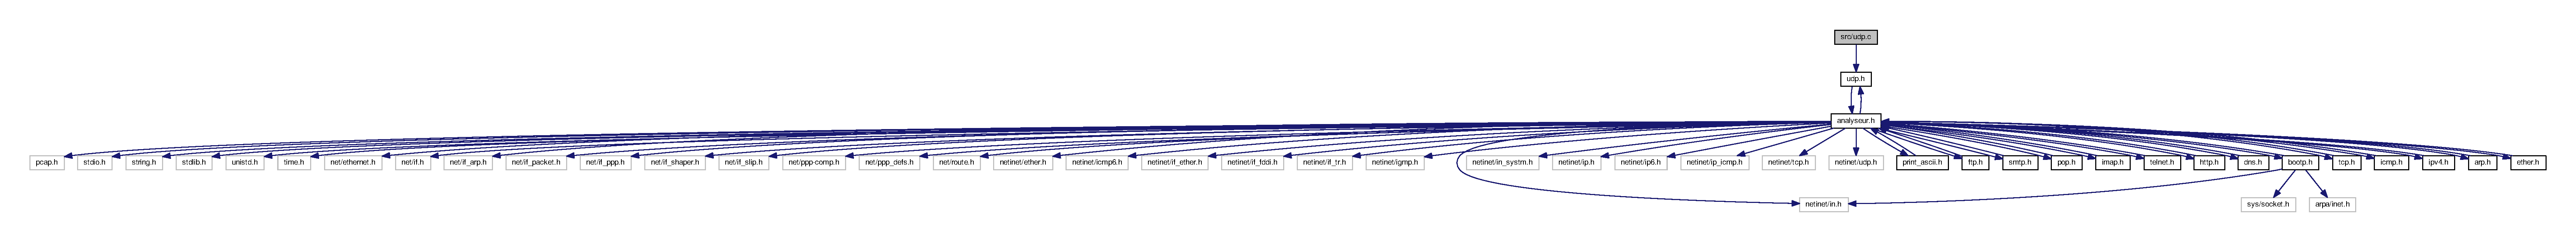
\includegraphics[width=350pt]{udp_8c__incl}
\end{center}
\end{figure}
\subsection*{Functions}
\begin{DoxyCompactItemize}
\item 
void \hyperlink{udp_8c_a533989bc1ee408051a2135fbc5173cd8}{affichage\+\_\+udp} (\hyperlink{struct_user}{User} $\ast$user, \hyperlink{analyseur_8h_a450cdf739df0886778ce02bd0ab86b63}{Udp\+Hdr} $\ast$udp)
\item 
void \hyperlink{udp_8c_ab2fc3a9e0c52a51f5d3fd3f771bcc40c}{analyse\+\_\+udp} (\hyperlink{struct_user}{User} $\ast$user, const u\+\_\+char $\ast$bytes)
\end{DoxyCompactItemize}


\subsection{Function Documentation}
\index{udp.\+c@{udp.\+c}!affichage\+\_\+udp@{affichage\+\_\+udp}}
\index{affichage\+\_\+udp@{affichage\+\_\+udp}!udp.\+c@{udp.\+c}}
\subsubsection[{\texorpdfstring{affichage\+\_\+udp(\+User $\ast$user, Udp\+Hdr $\ast$udp)}{affichage_udp(User *user, UdpHdr *udp)}}]{\setlength{\rightskip}{0pt plus 5cm}void affichage\+\_\+udp (
\begin{DoxyParamCaption}
\item[{{\bf User} $\ast$}]{user, }
\item[{{\bf Udp\+Hdr} $\ast$}]{udp}
\end{DoxyParamCaption}
)}\hypertarget{udp_8c_a533989bc1ee408051a2135fbc5173cd8}{}\label{udp_8c_a533989bc1ee408051a2135fbc5173cd8}
\index{udp.\+c@{udp.\+c}!analyse\+\_\+udp@{analyse\+\_\+udp}}
\index{analyse\+\_\+udp@{analyse\+\_\+udp}!udp.\+c@{udp.\+c}}
\subsubsection[{\texorpdfstring{analyse\+\_\+udp(\+User $\ast$user, const u\+\_\+char $\ast$bytes)}{analyse_udp(User *user, const u_char *bytes)}}]{\setlength{\rightskip}{0pt plus 5cm}void analyse\+\_\+udp (
\begin{DoxyParamCaption}
\item[{{\bf User} $\ast$}]{user, }
\item[{const u\+\_\+char $\ast$}]{bytes}
\end{DoxyParamCaption}
)}\hypertarget{udp_8c_ab2fc3a9e0c52a51f5d3fd3f771bcc40c}{}\label{udp_8c_ab2fc3a9e0c52a51f5d3fd3f771bcc40c}

\hypertarget{udp_8h}{}\section{src/udp.h File Reference}
\label{udp_8h}\index{src/udp.\+h@{src/udp.\+h}}
{\ttfamily \#include \char`\"{}analyseur.\+h\char`\"{}}\\*
Include dependency graph for udp.\+h\+:
\nopagebreak
\begin{figure}[H]
\begin{center}
\leavevmode
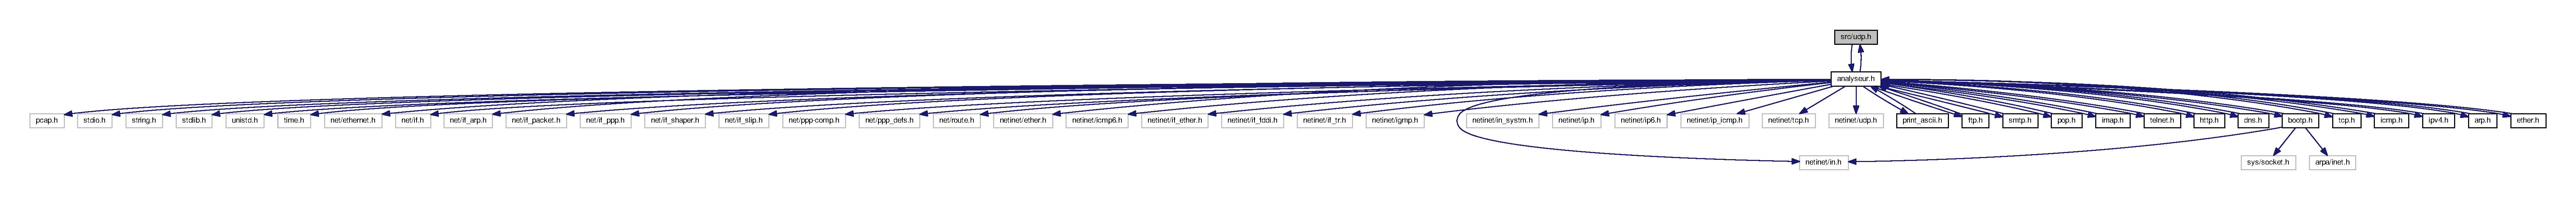
\includegraphics[width=350pt]{udp_8h__incl}
\end{center}
\end{figure}
This graph shows which files directly or indirectly include this file\+:
\nopagebreak
\begin{figure}[H]
\begin{center}
\leavevmode
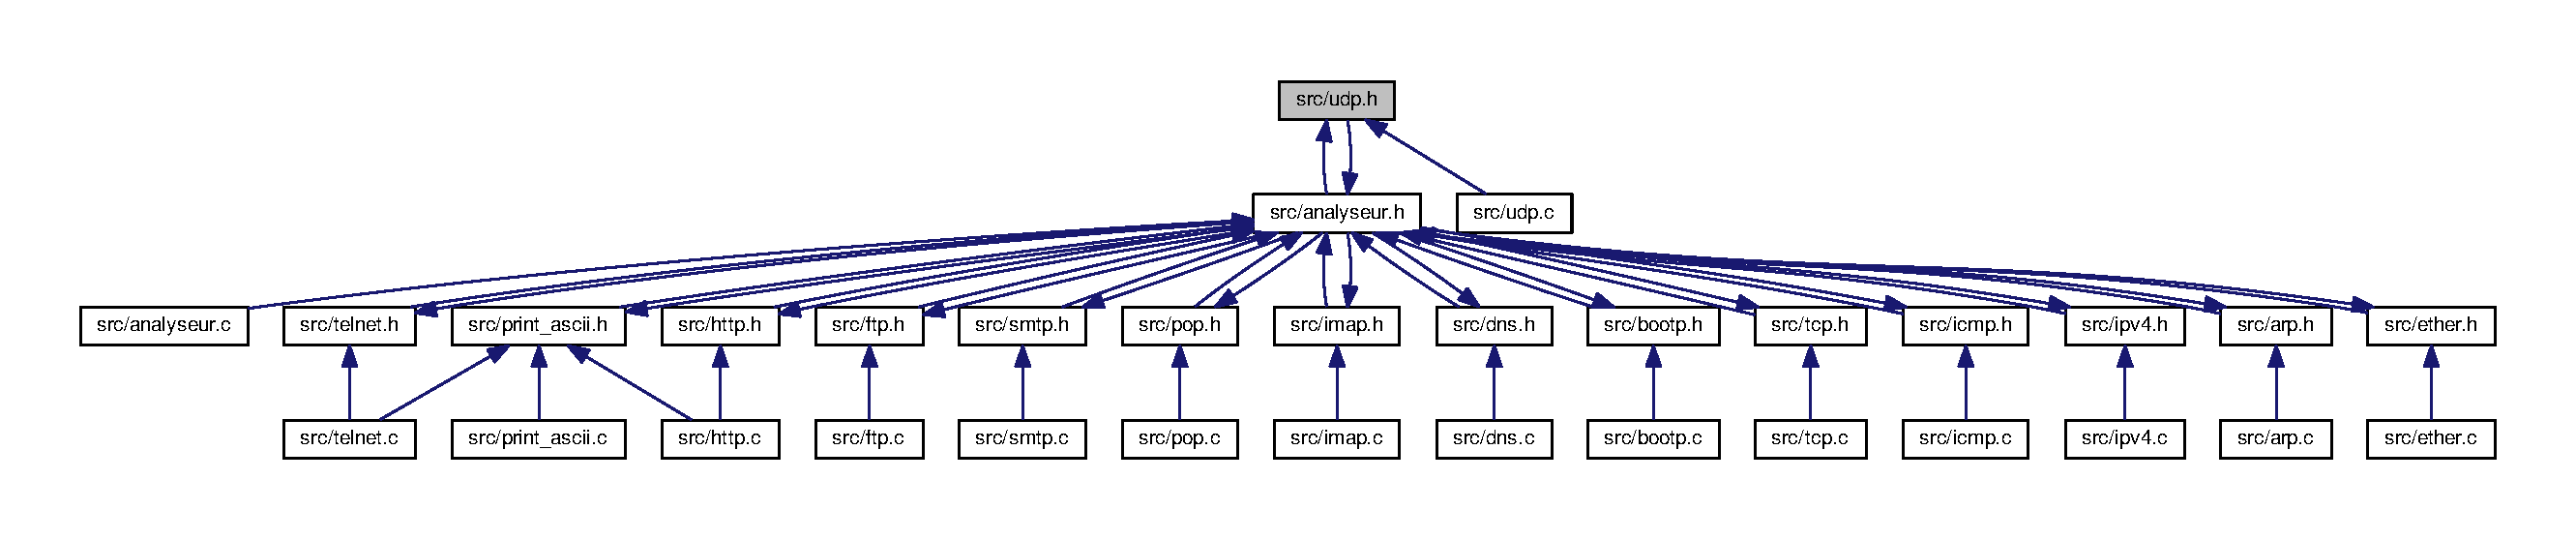
\includegraphics[width=350pt]{udp_8h__dep__incl}
\end{center}
\end{figure}
\subsection*{Functions}
\begin{DoxyCompactItemize}
\item 
void \hyperlink{udp_8h_ab2fc3a9e0c52a51f5d3fd3f771bcc40c}{analyse\+\_\+udp} (\hyperlink{struct_user}{User} $\ast$user, const u\+\_\+char $\ast$bytes)
\end{DoxyCompactItemize}


\subsection{Function Documentation}
\index{udp.\+h@{udp.\+h}!analyse\+\_\+udp@{analyse\+\_\+udp}}
\index{analyse\+\_\+udp@{analyse\+\_\+udp}!udp.\+h@{udp.\+h}}
\subsubsection[{\texorpdfstring{analyse\+\_\+udp(\+User $\ast$user, const u\+\_\+char $\ast$bytes)}{analyse_udp(User *user, const u_char *bytes)}}]{\setlength{\rightskip}{0pt plus 5cm}void analyse\+\_\+udp (
\begin{DoxyParamCaption}
\item[{{\bf User} $\ast$}]{user, }
\item[{const u\+\_\+char $\ast$}]{bytes}
\end{DoxyParamCaption}
)}\hypertarget{udp_8h_ab2fc3a9e0c52a51f5d3fd3f771bcc40c}{}\label{udp_8h_ab2fc3a9e0c52a51f5d3fd3f771bcc40c}

%--- End generated contents ---

% Index
\backmatter
\newpage
\phantomsection
\clearemptydoublepage
\addcontentsline{toc}{chapter}{Index}
\printindex

\end{document}
